\documentclass[12pt,a4paper]{article}
\usepackage{xecyr}
\usepackage{polyglossia}
\setdefaultlanguage{russian}
\setotherlanguage{english}
\usepackage{fancyvrb}

\usepackage{indentfirst}

\usepackage[margin=.7in]{geometry}
\setlength{\oddsidemargin}{0in}
%\setlength{\evensidemargin}{0.0in}

\usepackage{amsmath}
\usepackage{mathtext}
\usepackage{hyperref}
%\usepackage{ucs}
%\usepackage[t2a]{fontenc}
%\usepackage[utf8x]{inputenc}
%\usepackage[english,russian]{babel}
\usepackage{graphicx}

\setmainfont[Mapping=tex-text]{Liberation Sans}
\setmonofont{Inconsolata}
\renewcommand\scriptsize{\@setfontsize\scriptsize\@ixpt{11pt}}
%\setmathfont{Cambria Math}


\title{Введение в асинхронное программирование и Twisted}

\author{Dave Peticolas\\перевод Nina Evseenko}

\date{}

%\DefineVerbatimEnvironment{verbatim}{Verbatim}numbers=left,numbersep=5pt,frame=lines,framerule=0.8mm}

\nonfrenchspacing

\begin{document}

%\fvset{numbers=left,numbersep=5pt,frame=lines,framerule=0.8mm, fontsize=\large}
  
\maketitle
\thispagestyle{empty}
\eject

\tableofcontents

\eject

\clearpage 
% part 1
\section{С чего мы начнем вначале\label{sec:part1}}



    Данная статья является переводом. Оригинал, который можно найти на странице  
\href{http://krondo.com/?page\_id=1327}{Twisted Introduction},
был написан Dave Peticolas.


\subsection{Предисловие}


    В рассылке Twisted не так давно появился вопрос:  
можно ли где-нибудь найти описание, которое 
позволит быстро овладеть техникой использования Twisted? 
На данный момент такого описания не существует, и данное 
руководство им не является.


Если вы новичок в асинхронном программировании, то  
лучше изучать основные принципы постепенно. 
Исходя из продолжительного опыта использования Twisted и 
познания всех тонкостей и сложностей, данное пособие начинается с 
общего понятия модели асинхронного программирования. 
Большая часть кода Twisted понятна и 
хорошо написана, документация на сайте хорошая, по меньшей 
мере с точки зрения стандартов свободного ПО. Но без понятия модели, 
чтение кода Twisted или кода, использующего Twisted, или даже чтение 
документации, превратится в головную боль.


Таким образом, первые главы помогают 
осознать модель асинхронного программирования, а последующие - 
постичь особенности программирования с использованием Twisted. 
В самом начале мы совсем не будем использовать Twisted. 
Вместо этого, для иллюстрации функционирования асинхронной системы 
мы будем использовать простые программы на Python'е. И как только мы 
начнем использовать Twisted, мы начнем с очень низкого уровня, который 
вы не использовали бы в повседневном программировании. Twisted - 
высоко абстрактная система, и это дает вам огромное преимущество при решении 
проблем. Но, когда вы изучаете Twisted, в особенности, когда вы 
пытаетесь понять как Twisted реально работает, многоуровневые абстракции могут 
быть препятствием. Поэтому мы начнем с самых основ.


После того, как вы осознаете модель, вам будет проще 
читать документацию и исходный код Twisted. Так что - начнем. 


\subsection{Модели}


    Мы начнем с рассмотрения двух похожих моделей,
для того чтобы сравнить с ними асинхронную модель.
Для иллюстрации мы представим программу, которая
состоит из трех концептуально отличных задач,
которые должны быть выполнены, для того чтобы программа
завершилась. Мы конкретизируем эти задачи позже, сейчас
мы не будем говорить ничего о них, кроме того, что программа
должна выполнить эти задачи. Заметьте, что термин ``задача'' 
используется не в техническом смысле: ``нечто, что нужно выполнить''.



Первая модель, которую мы рассмотрим, - однопоточная синхронная модель, изображенная 
на рисунке \ref{fig:sync} ниже:

% fig1
\begin{figure}[h]
\begin{center}
    \includegraphics[height=0.3\textheight]{images/sync.pdf}
\end{center}
    \caption{Синхронная модель\label{fig:sync}}
\end{figure}

Это самый простой стиль программирования. Одновременно выполняется только одна задача, 
следующая задача выполняется только после того, как предыдущая завершилась. И, если 
задачи всегда выполняются в определенном порядке, то запуск следующей задачи 
может осуществиться, если все предыдущие задачи завершились без ошибок.


Мы можем сравнить синхронную модель с многопоточной моделью, изображенной 
на рисунке \ref{fig:threaded}:

% fig2
\begin{figure}[h]
\begin{center}
    \includegraphics[width=0.5\textwidth]{images/threaded.pdf}
\end{center}
    \caption{Модель на основе потоков\label{fig:threaded}}
\end{figure}

В этой модели каждая задача выполняется в
отдельном потоке. Потоки управляются операционной системой, и в
случае наличия нескольких процессоров и/или ядер, 
могут выполняться параллельно, или их выполнение
может чередоваться в случае одного процессора. Смысл в том, что
в тредовой модели деталями управляет операционная система, и 
программист просто думает в терминах независимых потоков инструкций,
которые могут выполняться одновременно. Хотя диаграмма простая, на
практике потоковые программы могут быть достаточно сложными,
поскольку нужно координировать потоки между собой. Потоковая координация и
взаимодействие являются отдельной, достаточно сложной темой.

Некоторые программы реализуют параллельность, используя несколько
процессов вместо нескольких потоков. Хотя, с точки зрения реализации есть
отличия, для наших целей это одна и та же модель, как на рисунке \ref{fig:threaded}.


Теперь мы можем перейти к асинхронной модели на рисунке \ref{fig:async}:

% fig3
\begin{figure}[h]
\begin{center}
    \includegraphics[height=0.3\textheight]{images/async.pdf}
\end{center}
    \caption{Acинхронная модель\label{fig:async}}
\end{figure}

В этой модели задачи выполняются поочередно в одном потоке. 
Это проще, чем в случае потоков, поскольку программист всегда знает, что
когда одна задача выполняется, другая - нет. Хотя в однопроцессорной системе
в потоковой программе задачи также будут выполняться поочередно, программист,
использующий потоки, все равно должен думать в терминах рисунка \ref{fig:threaded},
а не \ref{fig:async}, чтобы программа работала корректно при переходе
на многопроцессорную систему. Но однопоточная асинхронная система всегда
будет чередовать выполнение задач даже на многопроцессорной системе.


Существует еще одно отличие между асинхронной и потоковой моделями.
В потоковой модели решение приостановить один поток и выполнить другой
в большей степени не регулируется программистом. Скорее, это контролируется
операционной системой, и программист должен предполагать, что поток
может приостановиться и смениться другим практически в любой момент времени.
Что отличается от задач в асинхронной модели, которые выполняются до того момента,
когда явно не передают контроль другим задачам. Это значительно проще, чем
в случае потоков.


Заметим, что возможно смешивать асинхронные и потоковые модели, и использовать
оба варианта в одной системе. Но, для большей части этого введения,
мы будем придерживаться ``чистых`` асинхронных систем с управлением в один поток.


\subsection{Мотивация}


    Мы увидели, что асинхронная модель проще, чем потоковая, поскольку 
есть только единственный поток инструкций и задач, который явно передает 
управление, вместо приостановки в произвольный момент времени. Но 
асинхронная модель является явно более сложной, чем синхронная. 


Программист должен организовать задачу как последовательность 
маленьких шагов, которые периодически запускаются.


И, если одна задача использует вывод другой, то зависящая 
задача должна быть написана так, чтобы уметь принимать на вход  
результат по порциям, вместо одного большого куска.


Поскольку здесь нет параллельности, что видно из 
наших диаграмм, то асинхронная программа будет 
выполняться также долго как и синхронная, возможно дольше, 
так как асинхронная программа может быть
хуже с точки зрения локальности ссылок.


Так почему же мы бы выбрали асинхронную модель? 
Существует по меньшей мере две причины. 
Первая - если одна или более задач отвечают за реализацию интерфейса, 
то путем чередования задач, система сможет отвечать 
на пользовательский ввод даже тогда, когда в ``фоне'' выполняется 
другая задача. Так как фоновые задачи не могут выполниться быстрее, 
система будет более вежливой для того, кто ее использует. 
Однако, существуют условия, когда асинхронная система 
будет лучше по сравнению с синхронной, иногда намного, в смысле 
выполнения всех задач за более короткий промежуток времени.
Эти условия связаны с задачами, которые вынуждены ожидать событий 
или блокироваться, как это изображено на рисунке \ref{fig:block}: 

% fig4
\begin{figure}[h]
\begin{center}
    \includegraphics[height=0.3\textheight]{images/block.pdf}
\end{center}
    \caption{Блокирование в синхронной программе\label{fig:block}}
\end{figure}

На рисунке серые секции представляют собой периоды времени, 
когда определенная задача ожидает (блокируется) и не выполняется. 
Почему же задача может быть заблокирована? Частая причина - ожидание 
выполнения  ввода-вывода, связанное с перенесением 
данных из или во внешнее устройство. Обычный процессор может 
управлять переносом данных на порядок быстрее, по сравнению с максимальной 
скоростью переноса данных для диска или сети. Таким образом, синхронная 
программа, которая выполняет много операций ввода-вывода, будет 
часто блокироваться в момент обращения к диску или сети. Такая синхронная 
программа часто называется блокирующаяся программа (blocking program).


Заметьте, что на рисунке \ref{fig:block} изображена блокирующаяся программа, 
которая немного похожа на асинхронную программу на рисунке \ref{fig:async}. 
Это не совпадение. Основная идея в асинхронной модели - это то, что, когда  
асинхронная программа сталкивается с тем, что блокирует синхронную 
программу, асинхронная будет выполняться. Асинхронная программа будет 
``блокироваться'' только тогда, когда нет задач на выполнение, поэтому 
такая программа называется неблокирующейся (non-blocking program). 
И каждое переключение с одной задачи на другую соответствует тому, что 
первая задача или выполнилась, или находится в месте, где она заблокирована. 
С большим количеством потенциально блокирующихся задач, 
асинхронная программа может превосходить синхронную тем, что проводит 
в целом меньше времени ожидая.


По сравнению с синхронной моделью, асинхронная модель лучше когда:

\begin{enumerate}

\item Когда есть много задач таких, что почти всегда есть по меньшей мере 
    одна задача, которая может выполняться.
\item Задачи выполняют много операций ввода-вывода, приводя к тому, что
    синхронная задача проводит много времени впустую, блокируясь, в то время 
    когда другие задачи могли бы выполняться.
\item Задачи независимы друг от друга и не нуждаются во 
    взаимодействии.
\end{enumerate}


Эти условия почти полностью характеризуют типичный сетевой сервер (например, 
web сервер) в среде клиент-сервер. Каждая задача представляет собой один 
клиентский запрос с операциями ввода-вывода в форме получения запроса и 
отправления ответа. И клиентские запросы по большому счету независимы. 
Так что реализация сетевого сервера является подходящим кандидатом для 
асинхронной модели, поэтому Twisted - это одна из первых и передовых 
сетевых библиотек. 


\subsection{Дальше и больше}


    Это окончание первой части. Во второй части мы будем писать 
некоторые сетевые программы, обе - блокирующиеся и неблокирующиеся, 
настолько простые, насколько это возможно (без использования Twisted), 
для того, чтобы осознать как действительно работает 
асинхронная программа, написанная на Python'е.


 \clearpage
\clearpage 
% part 2
\section{Медленная поэзия и апокалипсис\label{sec:part2}}


    На этот раз мы запачкаем наши руки и напишем некоторый код. Но сначала - 
некоторые предположения.


\subsection{Предположения о навыках}


    Предполагается, что вы имеете некоторые навыки написания 
синхронных программ на Python'е и немного знаете о 
сокетном программировании на Python'е. Если вы никогда раньше не 
использовали сокеты, вы можете почитать 
\href{http://docs.python.org/library/socket.html#module-socket}{документацию о Python-модуле socket}, 
особенно примеры ближе к концу. Если вы никогда раньше не 
использовали Python, то все остальное вам, вероятно, покажется странным.  


\subsection{Предположения о компьютере}


    Примеры разрабатывались и отлаживались на Linux'е. 
Возможно, что код работает 
под другие Unix подобные системы (Mac OSX или FreeBSD).


Далее предполагается, что вы установили относительно свежые  
версии 
\href{http://python.org/download}{Python} и 
\href{http://twistedmatrix.com/trac/wiki/Downloads}{Twisted}. 
Примеры разрабатывались с использованием 
Python 2.5 и Twisted 8.2.0.


Вы можете запускать все примеры на одном компьютере или 
сконфигурировать их для запуска по сети на 
нескольких машинах. Но для изучения основных механизмов 
асинхронного программирования использование одной 
машины предпотчтительнее.


Код с примерами доступен ввиде  
\href{http://github.com/jdavisp3/twisted-intro/zipball/master}{zip} или 
\href{http://github.com/jdavisp3/twisted-intro/tarball/master}{tar} файла, или как 
\href{http://github.com/jdavisp3/twisted-intro/tree/master}{git репозиторий}. 
Если вы можете использовать git 
или другую систему контроля версий, которая может читать 
git репозиторий, то рекомендуется использовать этот метод, 
так как примеры время от времени обновляются, и в этом случае 
обновление будет осуществляться гораздо проще. Репозиторий 
помимо всего прочего  
включает исходники рисунков в формате SVG. 
Клонировать репозиторий можно следующим образом: 

\begin{scriptsize}\begin{verbatim}
git clone git://github.com/jdavisp3/twisted-intro.git
\end{verbatim}\end{scriptsize}

И последнее предположение: наличие нескольких консолей, 
открытых в директории с примерами (в одной из них предполагается 
открытым файл README).


\subsection{Медленная поэзия}


    Хотя процессоры намного быстрее, чем сети, 
а большинство сетей все же намного быстрее, чем мозг, 
или по меньшей мере быстрее, чем скорость движения 
глаз. Сложно получить заметную задержку в сети, особенно, в случае 
одной машины и байтов, проносящихся со свистом на  
\href{http://en.wikipedia.org/wiki/Loopback}{loopback интерфейсе}. 
То что нам нужно - медленный сервер, 
с искуственными задержками, которые мы можем менять для 
изучения их воздействия. Поскольку серверы должны что-то 
обслуживать, то наш сервер будет обслуживать поэзию. 
В исходниках примеров находится директория poetry с поэзией авторов 
\href{http://en.wikipedia.org/wiki/Donne}{John Donne},
\href{http://en.wikipedia.org/wiki/Yeats}{W.B. Yeats}, 
\href{http://en.wikipedia.org/wiki/Poe}{Edgar Allen Poe}. 
Конечно же, вы можете использовать свои собственные поэмы. 


Медленный поэтический сервер реализован в 
\href{http://github.com/jdavisp3/twisted-intro/blob/master/blocking-server/slowpoetry.py}{blocking-server/slowpoetry.py}. 
Вы можете запустить пример сервера следующим образом:

\begin{scriptsize}\begin{verbatim}
python blocking-server/slowpoetry.py poetry/ecstasy.txt
\end{verbatim}\end{scriptsize}


Эта команда запустит блокирующий сервер с 
поэмой “Ecstasy” John Donne. Пойдем дальше и посмотрим на 
исходный код блокирующего сервера. Как можно заметить, в 
коде не используется Twisted, только основные сокетные 
операции. Сервер отправляет ограниченное количество 
байт за раз, с фиксированной временной задержкой между ними. 
По умолчанию, сервер отправляет 10 байт каждые 0.1 секунды, 
но вы можете поменять эти параметры с помощью опций 
командной строки \textit{\symbol{45}\symbol{45}num-bytes} и 
\textit{\symbol{45}\symbol{45}delay}. Например, чтобы 
отправлять 50 байт каждые 5 секунд, нужно запустить: 

\begin{scriptsize}\begin{verbatim}
python blocking-server/slowpoetry.py --num-bytes 50 --delay 5 poetry/ecstasy.txt
\end{verbatim}\end{scriptsize}


Когда сервер запускается, он печатает номер порта, который он 
слушает. По умолчанию, это первый доступный случайный порт на вашей машине. 
Запуская сервер с различными настройками, может понадобится использовать 
тот же порт, что и до этого, для того, чтобы не нужно было 
перенастраивать клиент. Вы можете задать определенный порт следующим образом:

\begin{scriptsize}\begin{verbatim}
python blocking-server/slowpoetry.py --port 10000 poetry/ecstasy.txt
\end{verbatim}\end{scriptsize}

Если у вас есть программа 
\href{http://netcat.sourceforge.net/}{netcat} (или nc), можно протестировать 
запущенный сервер следующим образом:

\begin{scriptsize}\begin{verbatim}
netcat localhost 10000
\end{verbatim}\end{scriptsize}


При запущенном сервере вы увидите медленно ползущую 
вниз по экрану поэму. Экстаз! Вы также заметите, что сервер 
печатает строки с количеством отосланных байт. Сразу после того, как 
поэма была отослана, сервер закрывает соединение.


По умолчанию, сервер слушает только локальный "loopback" 
интерфейс. Если вы хотите получить доступ к серверу с 
другой машины, вы можете задать сетевой интерфейс через 
опцию --iface.


Сервер не только медленно отправляет поэму, по коду видно, что 
во время отправления сервером поэмы одному клиенту, другие 
клиенты должны ожидать окончания скачивания поэмы первым клиентом 
до того, как другие смогут получить хотя бы первую строку. 
Это реально медленный сервер и не особо полезен, кроме как 
в обучающих целях. 


С другой стороны, если большинство пемиссемистичных 
людей из 
\href{http://www.peakoil.net/}{Peak Oil} правы, и нашему миру грозит 
глобальный энергетический и социальный кризис, то, однажды, 
низкопропускной и маломощный сервер может стать именно тем, что нам 
нужно. Представьте, что после длительного дня забот о ваших 
садах, производстве собственной одежды, обслуживания 
Центрального Организационного Комитета Вашей комунны, борьбы 
с радиокативными зомби, бродящими по пост-апокалиптическим 
пустошам, вы сможете покрутить ваш генератор и скачать 
несколько строк высокой культуры из исчезнувшей цивилизации. 
Вот тогда наш сервер реально вcтупит в свои права. 


\subsection{Блокирующий клиент}


    Также в исходных кодах можно найти пример блокирующего 
клиента, который скачивает поэмы из серверов одну за 
другой. Давайте дадим нашему клиенту три задачи для 
выполнения так, как это изображено на рисунке \ref{fig:sync}. 
Сначала мы запустим три сервера, обслуживающих три 
различных поэмы:

\begin{scriptsize}\begin{verbatim}
python blocking-server/slowpoetry.py --port 10000 poetry/ecstasy.txt --num-bytes 30
python blocking-server/slowpoetry.py --port 10001 poetry/fascination.txt
python blocking-server/slowpoetry.py --port 10002 poetry/science.txt
\end{verbatim}\end{scriptsize}


Вы можете выбрать другие номера портов, если те, 
что выбраны выше, уже используются в вашей системе. 
Заметьте, что первый сервер использует chunk'и по 
30 байт, вместо 10, что установлены по умолчанию, 
поскольку поэма, которую он обслуживает  примерно 
в три раза длиньше остальных. При таких настройках 
скачивание каждой из них должно завершаться 
приблизительно в одно и тоже время.


Теперь мы можем запустить блокирующий клиент из 
\href{http://github.com/jdavisp3/twisted-intro/blob/master/blocking-client/get-poetry.py}{blocking-client/get-poetry.py}, 
для того, чтобы скачать немного поэзии. Запустите клиент следующим образом:

\begin{scriptsize}\begin{verbatim}
python blocking-client/get-poetry.py 10000 10001 10002
\end{verbatim}\end{scriptsize}


Вы также можете поменять номера портов, если сервера 
слушают на других портах. Поскольку мы имеем дело с 
блокирующим клиентом, то он будет скачивать одну поэму 
из каждого порта по очереди, ожидая пока поэма будет 
полностью получена до того, как начать скачивать 
следующую поэму. Вместо печати поэм, блокирующий клиент 
выводит нечто вроде: 

\begin{scriptsize}\begin{verbatim}
Task 1: get poetry from: 127.0.0.1:10000
Task 1: got 3003 bytes of poetry from 127.0.0.1:10000 in 0:00:10.126361
Task 2: get poetry from: 127.0.0.1:10001
Task 2: got 623 bytes of poetry from 127.0.0.1:10001 in 0:00:06.321777
Task 3: get poetry from: 127.0.0.1:10002
Task 3: got 653 bytes of poetry from 127.0.0.1:10002 in 0:00:06.617523
Got 3 poems in 0:00:23.065661
\end{verbatim}\end{scriptsize}

Это очень похоже на текстовую версию рисунка \ref{fig:sync}, где 
каждая задача качает одну поэму. В вашем выводе времена скачиваний  
могут немного отличаться. Ими можно вариьровать через параметр сервера 
\textit{\symbol{45}\symbol{45}delay}. 
Попробуйте поменять его и увидеть как меняется время скачивания.


Теперь можно посмотреть на исходный код блокирующего сервера и 
клиента и отметить места в коде, где они блокируются при 
отправлении или получении сетевых данных.


\subsection{Асинхронный клиент}


    Давайте теперь посмотрим на реализацию простого 
асинхронного клиента, написанного без ипользования 
Twisted. Сначала давайте его запустим. Запустите три сервера, 
как мы это делали выше. 
Если они все еще запущены, то мы можем снова их 
использовать. Теперь запустим асинхронный клиент, 
расположенный в 
\href{http://github.com/jdavisp3/twisted-intro/blob/master/async-client/get-poetry.py}{async-client/get-poetry.py},  
как написано ниже:

\begin{scriptsize}\begin{verbatim}
python async-client/get-poetry.py 10000 10001 10002
\end{verbatim}\end{scriptsize}


В результате получится примерно такой вывод:

\begin{scriptsize}\begin{verbatim}
Task 1: got 30 bytes of poetry from 127.0.0.1:10000
Task 2: got 10 bytes of poetry from 127.0.0.1:10001
Task 3: got 10 bytes of poetry from 127.0.0.1:10002
Task 1: got 30 bytes of poetry from 127.0.0.1:10000
Task 2: got 10 bytes of poetry from 127.0.0.1:10001
...
Task 1: 3003 bytes of poetry
Task 2: 623 bytes of poetry
Task 3: 653 bytes of poetry
Got 3 poems in 0:00:10.133169
\end{verbatim}\end{scriptsize}

На этот раз вывод намного длиньше, поскольку клиент выводит 
строку после каждого скачивания порции данных с любого сервера. 
Сервера, как и раньше, понемногу отдают поэзию. 
Заметьте, что выполнение отдельных задач чередуется, как это изображено на 
рисунке \ref{fig:async}.


Попробуйте поменять опцию \textit{\symbol{45}\symbol{45}delay} 
для серверов (например, сделать 
один сервер медленнее, чем остальные) для того, чтобы увидеть 
как асинхронный клиент автоматически "подстроится" под скорость 
медленных серверов, в тоже время успевая за быстрыми серверами. 
Это асинхронность в действии. 


Также заметьте, что при найстройках сервера, которые были установлены 
выше, асинхронный 
клиент завершается примерно за 10 секунд, в то время как 
синхронному клиенту требуется примерно 23 секунды для получения 
всех поэм. Теперь вернемся к отличиям между рисунками \ref{fig:async} и 
\ref{fig:block}. Тратя меньше времени на блокирование, наш 
асинхронный клиент может скачать все поэмы за более короткий промежуток 
времени, поскольку он переключается между всеми медленными серверами.


Технически, наш асинхронный клиент выполняет блокирующую операцию: 
он пишет в стандартный вывод, используя оператор print! Это не 
является проблемой в нашем случае. На локальной машине с 
терминальным shell'ом, готовым принять вывод, оператор print 
не будет реально блокироваться и будет выволняться досточно быстро 
по сравнению с нашими медленными серверами. Но, если бы мы захотели, 
чтобы наша программа была частью pipeline и все еще выполнялась 
асинхронно, нам нужно было бы использовать асинхронный ввод-вывод 
для стандартного ввода и вывода. Twisted имеет модули, реализующие это, 
но для простоты, мы будем использовать 
оператор print, даже в программах, написанных с использованием Twisted.


\subsection{Пристальный взгляд}


    Теперь давайте посмотрим на исходный код асинхронного клиента. 
Отметим основные отличия между ним и синхронным клиентом:

\begin{enumerate}
\item Вместо соединения только с одним сервером в один момент времени  
асинхронный клиент соединяется со всеми серверами одновременно.

\item Сокетные объекты, использованные для соединения, устанавливаются в неблокирующее 
состояние с использованием вызова setblocking(0).

\item Используется метод select из модуля 
\href{http://docs.python.org/library/select.html#module-select}{select} для ожидания (блокирования) 
до того момента, когда хотя бы один из сокетов готов отдать некоторую 
порцию данных.

\item При чтении данных из серверов мы читаем по максимуму до 
момента блокирования сокета, затем переходим к чтению данных 
из следующего имеющегося готового к чтению сокета. 
\end{enumerate}


Ядром асинхронного клиента является внешний цикл в 
функции get\_poetry. Этот цикл можно разбить на 
несколько шагов:

\begin{enumerate}
\item Ожидание (блокирование) всех открытых сокетов с использованием select'а, 
до тех пор пока один или более сокетов будут иметь данные для считывания. 
\item Для каждого сокета с готовыми для считывания данными, прочитать их, но только 
в количестве, доступном на данный момент, чтобы избежать 
\href{http://en.wikipedia.org/wiki/Asynchronous\_I/O}{блокирования}.
\item Повторять шаги выше до момента закрытия сокетов.
\end{enumerate}


Синхронный клиент также имеет цикл (в функции main), но 
при каждой итерации цикла в синхронном клиенте скачивается полностью 
одна поэма. В то время как при каждой итерации асинхронного 
клиента скачиваются куски поэм. И мы не знаем, 
над какими из них мы будем работать в данной итерации, или 
сколько данных мы получим от каждой из них. Все это зависит от 
относительных скоростей серверов и состояния сети. Мы только 
позволяем select'у сообщать нам о том, какие сокеты готовы на чтение, 
и читаем столько данных, сколько можем из каждого сокета, не блокируясь.


Если бы синхронный клиент соединялся бы 
с фиксированным количеством серверов (скажем тремя), 
нам бы совершенно не понадобился внешний цикл, поскольку 
можно было бы последовательно вызвать три раза 
функцию get\_poetry. Но асинхронный клиент не может 
обходиться без внешнего цикла, поскольку нужно одновременно 
опрашивать все сокеты и обрабатывать столько 
данных, сколько было доставлено за заданную итерацию. 


Использование подобного цикла, ожидающего событий и 
управляющего ими, является общепринятым, и известно как 
\href{http://en.wikipedia.org/wiki/Reactor\_pattern}{шаблон проектирования reactor}. 
Изложенное выше проиллюстрировано на рисунке \ref{fig:reactor-1}:

% fig5
\begin{figure}[h]
\begin{center}
    \includegraphics[width=0.3\textwidth]{images/reactor-1.pdf}
\end{center}
    \caption{Цикл reactor'а\label{fig:reactor-1}}
\end{figure}

\eject

Цикл является “reactor'ным”, поскольку он ожидает событий 
и затем реагирует на них. По этой причине, такой цикл 
известен также как "event loop". Поскольку реактивные 
системы зачастую ожидают ввода-вывода, такие циклы зачастую 
называют 
\href{http://en.wikipedia.org/wiki/Asynchronous\_I/O#Select.28.2Fpoll.29\_loops}{select циклы}, 
поскольку вызов select используется для ожидания ввода-вывода. 
Таким образом в select циклах, "событием" является момент, когда 
сокет становится доступным на чтение или запись. Надо отметить, что 
select - не единственный способ ожидания ввода-вывода, это один 
из самых старых (поэтому широко доступных) методов. Существует несколько 
более новых API, доступных на различных операционных системах, 
которые делают те же вещи, что и select, но имеют лучшую 
производительность. Но, невзирая на производительность, они все делают 
одно и тоже: берут множество сокетов (реально файловых дескрипторов) и 
блокируются до тех пор, пока один или более из них не станут готовы для 
операций ввода-вывода.  


Нужно отметить, что можно использовать select и его 
товарищей для простой проверки на готовность множества 
файловых дескрипторов для операций ввода-вывода без 
блокирования. Это свойство позволяет реагирующей системе (reactive system) 
выполнять что-либо, не являющееся вводом-выводом, 
внутри цикла. Но в реагирующих системах в основном вся работа 
связана с вводом-выводом, таким образом блокирование на 
всех файловых дескрипторах сохранит ресурсы процессора.


Говоря точно, цикл в нашем асинхронном клиенте не соответсвует 
шаблону проектирования reactor, поскольку логика в цикле не 
реализована отдельно от основной логики, которая является 
специфичной для поэтических серверов. Они просто перемешаны 
друг с другом. Реальная реализация шаблона проектирования reactor 
реализовывала бы цикл как отдельную абстракцию, способную:

\begin{enumerate}

\item Принимать множество файловых дескрипторов для выполнения 
операций ввода-вывода.

\item Циклически сообщать о том, когда любой из файловых дескриторов 
готов на чтение или запись. 

\end{enumerate}


А реально хорошая реализация шаблона проектирования reactor 
делала бы:

\begin{enumerate}

%   1. Handle all the weird corner cases that crop up on different systems.
\item Управление всеми проблемными случаями, которые происходят на 
различных системах.

%   2. Provide lots of nice abstractions to help you use the reactor with the least amount of effort.
\item Обеспечение множеством абстракций, помогающих использовать 
reactor с минимальными усилиями.

%   3. Provide implementations of public protocols that you can use out of the box.
\item Предоставление реализаций основных протоколов, которые можно тут же использовать.

\end{enumerate}

В целом, Twisted - это устойчивая, кросс-платформенная 
реализация шаблона проектирования reactor со 
множественными дополнениями. И в следующей главе мы 
начнем писать простые программы с использованием Twisted, 
так что сейчас мы движемся напрямую к получению поэзии со вкусом Twisted!


\subsection{Упражнения}

\begin{enumerate}

\item Проделайте несколько экспериментов с блокирующей 
и асинхронной версиями клиента, меняя количество и настройки 
поэтических серверов.

\item Может ли асинхронный клиент предоставить функцию get\_poetry, 
которая возвращала бы текст поэмы? Почему нет?

\item Если бы вы хотели реализовать функцию get\_poetry в 
асинхронном клиенте аналогичную синхронной версии, как бы 
это могло работать? Какие аргументы и возвращаемые значения  
были бы в этом случае?

\end{enumerate}



 \clearpage
\clearpage 
% part 3

\section{Наш первый взгляд на Twisted\label{sec:part3}}

\subsection{Ничего не делать - путь Twisted}

На данный момент мы нацелены на улучшение кода  
асинхронного поэтического клиента,  
используя Twisted. Cначала давайте напишем 
несколько простых Twisted программ,  
чтобы осознать cуть вещей. Как было упомянуто в главе 2,  
примеры были отлажены с использованием Twisted 8.2.0. API 
в Twisted меняется, но основные API, которые мы собираемся использовать 
меняются медленно, поэтому примеры 
будут актуальны и для cледующих релизов. Если у вас не 
установлен Twisted, вы можете получить его 
\href{http://twistedmatrix.com/trac/wiki/Downloads}{здесь}.


Самая простая Twisted программа представлена ниже. Код можно 
найти в директории с примерами в файле    
\href{http://github.com/jdavisp3/twisted-intro/blob/master/basic-twisted/simple.py}{basic-twisted/simple.py}. 

\begin{scriptsize}\begin{verbatim}
from twisted.internet import reactor
reactor.run()
\end{verbatim}\end{scriptsize}

Пример запускается следующим образом:

\begin{scriptsize}\begin{verbatim}
python basic-twisted/simple.py
\end{verbatim}\end{scriptsize}

В предыдущей главе мы выяснили, что Twisted - реализация шаблона проектирования 
\href{http://en.wikipedia.org/wiki/Reactor\_pattern}{Reactor}, 
таким образом Twisted содержит объект, который представляет reactor или 
event loop, который является ядром любой Twisted программы. Первая строка 
нашей программы импортирует объект reactor, чтобы его можно было   
использовать, вторая строка запускает цикл реактора. 


Программа выше ничего не делает. Остановить ее можно, 
нажав Ctrl-C, иначе она будет вечно ничего не делать. 
Обычно в цикле мониторятся на ввод-вывод какие-нибудь 
файловые дескрипторы (например, соединенные с поэтическим 
сервером). Позже, мы сделаем это, но сейчас 
цикл реактора простаивает. Заметьте, что это не 
\href{http://en.wikipedia.org/wiki/Busy\_waiting}{busy loop}, 
который реально выполняет цикл. Если посмотреть 
на загруженность процесса, то не будет видно никаких 
всплесков. Фактически, наша программа совсем не использует 
процессор. Вместо этого reactor простаивает наверху 
цикла рисунка \ref{fig:reactor-1}, ожидая события, которое 
никогда не произойдет (в реальности, ожидая возврата 
вызова select без файловых дескрипторов).


Сделаем несколько выводов:

\begin{enumerate}
\item Цикл реактора в Twisted запускается явно вызовом reactor.run().

\item Цикл реактора запускается в том же треде, где он 
был запущен. В примере выше, он был запущен в единственном main треде. 

\item После запуска цикл бесконечно продолжается.

\item Если нет задач, цикл реактора не потребляет процессор.

\item reactor явно не создается, он просто импортируется.
\end{enumerate}


Последний пункт стоит обсудить. Twisted reactor -  
\href{http://en.wikipedia.org/wiki/Singleton\_pattern}{Singleton}. 
Существует только один объект reactor, и он создается неявно при импорте. 
Если открыть модуль reactor в пакете twisted.internet, то кода там будет 
очень мало. Реальная реализация находится в другом файле:
\newline (\href{http://twistedmatrix.com/trac/browser/tags/releases/twisted-8.2.0/twisted/internet/selectreactor.py}{twisted.internet.selectreactor.py}).


В Twisted есть много различных реализаций реактора. Как было упомянуто 
в главе 2, вызов select'а - это один из способов ожидания событий на 
файловых дескрипторах. По умолчанию, Twisted использует select, 
но Twisted также включает и другие типы реакторов. Например, 
\href{http://twistedmatrix.com/trac/browser/tags/releases/twisted-8.2.0/twisted/internet/pollreactor.py}{twisted.internet.pollreactor}, который использует системный вызов 
\href{http://www.makelinux.net/ldd3/chp-6-sect-3.shtml}{poll} вместо 
select.


Для использования другого реактора нужно установить его до 
импортирования twisted.internet.reactor. Вот так можно 
установить pollreactor:

\begin{scriptsize}\begin{verbatim}
from twisted.internet import pollreactor
pollreactor.install()
\end{verbatim}\end{scriptsize}


Если проимпортировать twisted.internet.reactor без 
установки определенной реализации реактора, то 
Twisted установит reactor на основе select. 
По этой причине не импортируйте reactor в начале 
модулей, чтобы избежать случайной установки 
реактора по умолчанию, вместо этого импортируйте 
в том же месте, где собираетесь использовать.


Стоит заметить, что на момент написания статьи, Twisted двигается в 
сторону архитектуры, которая позволила бы использовать 
несколько реакторов одновременно. В такой схеме объект 
reactor мог бы подставляться как ссылка, а не как объект,  
импортированный из модуля.


Сейчас можно переписать нашу первую Twisted программу, 
используя pollreactor, которую можно найти в 
\href{http://github.com/jdavisp3/twisted-intro/blob/master/basic-twisted/simple-poll.py}{basic-twisted/simple-poll.py}:

\begin{scriptsize}\begin{verbatim}
from twisted.internet import pollreactor
pollreactor.install()

from twisted.internet import reactor
reactor.run()
\end{verbatim}\end{scriptsize}

Таким образом, мы имеем poll цикл, который ничего не делает, вместо 
ничего не делающего select цикла. 


Далее мы везде будем придерживаться реактора по умолчанию. Все 
реакторы Twisted делают одно и тоже.


\subsection{Привет, Twisted}

Давайте сделаем программу Twisted, которая что-нибудь делает. 
Например, программу, печатающую сообщение в окне терминала, 
после запуска цикла реактора:

\begin{scriptsize}\begin{verbatim}
def hello():
    print 'Hello from the reactor loop!'
    print 'Lately I feel like I\'m stuck in a rut.'

from twisted.internet import reactor

reactor.callWhenRunning(hello)

print 'Starting the reactor.'
reactor.run()
\end{verbatim}\end{scriptsize}

Код программы находится в 
\href{http://github.com/jdavisp3/twisted-intro/blob/master/basic-twisted/hello.py}{basic-twisted/hello.py}. 
После запуска получится следующий вывод:

\begin{scriptsize}\begin{verbatim}
Starting the reactor.
Hello from the reactor loop!
Lately I feel like I'm stuck in a rut.
\end{verbatim}\end{scriptsize}

Программу выше все еще надо завершать самостоятельно, 
поскольку она бесконечно выполняется после того, как напечатает 
строки выше.


Заметьте, что функция hello вызывается после того, как reactor 
начал выполняться. Это означает, что функция вызывается 
реактором, то есть код Twisted должен вызывать эту функцию. 
Это происходит благодаря вызову метода реактора callWhenRunning с 
ссылкой на функцию, которую должен вызвать Twisted. И, конечно же, 
мы должны вызвать callWhenRunning до того, как мы запустим 
reactor.


Термин callback означает ссылку на функцию (например, на 
функцию hello), которую мы 
передаем Twisted (или какой-то другой системе), 
которую Twisted будет использовать для того, чтобы "вызывать"  
в определенное время. В примере выше такой вызов происходит 
сразу же после того, как reactor запустится. Поскольку 
цикл в Twisted отделен от нашего кода, большинство 
взаимодействий между ядром реактора и логикой программы 
будет осуществляться через callback'и, которые 
мы передали Twisted, используя различные API.   


Мы можем увидеть то, как Twisted вызывает наш код, 
используя следующую программу:

\begin{scriptsize}\begin{verbatim}
import traceback

def stack():
    print 'The python stack:'
    traceback.print_stack()

from twisted.internet import reactor
reactor.callWhenRunning(stack)
reactor.run()
\end{verbatim}\end{scriptsize}


Код находится в 
\href{http://github.com/jdavisp3/twisted-intro/blob/master/basic-twisted/stack.py}{basic-twisted/stack.py}, 
и он напечатает что-то вроде этого:

\begin{scriptsize}\begin{verbatim}
The python stack:
...
  reactor.run() <-- This is where we called the reactor
...
...  <-- A bunch of Twisted function calls
...
  traceback.print_stack() <-- The second line in the stack function
\end{verbatim}\end{scriptsize}


Не обращайте внимание на все строки, просто 
осознайте взаимосвязь между вызовом  reactor.run() и 
нашим callback'ом. 


\subsection{Кто использует callback'и?}

Twisted не единственная система, которая использует callback'и. 
Более старые асинхронные Python системы 
\href{http://www.nightmare.com/medusa/}{Medusa} и 
\href{http://docs.python.org/library/asyncore.html#module-asyncore}{asyncore} 
также их используют. Помимо этого, многие GUI библиотеки, в том числе    
\href{http://gtk.org/}{GTK} и \href{http://qt.nokia.com/}{QT}, 
основаны на цикле реактора.


Отметим некоторые вещи:

\begin{enumerate}
\item Шаблон проектирования reactor однопоточный.
\item Реактивная система, подобная Twisted, реализует цикл 
реактора так, что наш код не должен его реализовывать.
\item Наш код должен реализовывать основную логику программы. 
\item Поскольку программа выполняется в одном потоке, 
цикл реактора будет вызывать наш код.
\item reactor не может знать наперед какую часть нашего кода нужно вызвать.
\end{enumerate}

Использование callback'ов, является неотъемлемой 
частью асинхронного программирования.

\eject

Рисунок \ref{fig:reactor-callback} показывает, что случается во время 
обратного вызова:

% fig6
\begin{figure}[h]
\begin{center}
    \includegraphics[width=0.5\textwidth]{images/reactor-callback.pdf}
    \caption{reactor, делающий обратный вызов\label{fig:reactor-callback}}
\end{center}
\end{figure}


Рисунок \ref{fig:reactor-callback} иллюстрирует некоторые важные особенности 
callback'ов:

\begin{enumerate}
\item Код нашего callback'а запускается в том же потоке, что и Twisted цикл.
\item Когда наши callback'и выполняются, цикл Twisted не выполняется. 
\item И наоборот.
\item Цикл реактора начинает выполняться после возврата из callback'ов.
\end{enumerate}


Во время вызова callback-функции, цикл Twisted 
блокируетяся на нашем коде. Поэтому нам следует 
убедиться, что код нашего callback'а не тратит 
время зря. То есть нам нужно избегать реализации 
блокирующего ввода-вывода в коде callback'ов. 
Иначе, использование реактора окажется бесмысленным. 
Twisted не имеет никаких специальных мер для 
предотвращения кода от блокирования, мы сами 
должны заботиться об этом. Как мы увидим позже, 
в большинстве случаев сетевого ввода-вывода нам не 
нужно беспокоится о блокировании, позволяя Twisted делать 
асинхронные взаимодействия за нас.  


Другие примеры потенциально блокирующих операций 
включают чтение и запись из несокетных файловых 
дескрипторов (побобных pipe) или ожидание завершения 
подпроцесса. Как вы будете переходить 
из блокирующихся к неблокирующимся операциям, зависит от того, 
что вы делаете, но зачастую есть уже реализованные Twisted API, 
которые могут помочь. Заметьте, что многие стандартные 
Python функции не имеют способа стать неблокирующимися. Например, 
вызов функции os.system всегда блокируется до тех пор, пока 
подпроцесс не остановится. При использовании Twisted, вам 
следует избегать os.system и отдать предпотчтение Twisted API 
для запуска подпроцессов.


\subsection{До свидания, Twisted}


В свою очередь, вы можете сказать реакторy Twisted 
остановить выполнение, используя метод stop. Но однажды 
остановленный reactor не может быть перезапущен, поэтому 
в основном это делается, когда программа завершается. 


В рассылке Twisted обсуждалась тема о том, чтобы сделать 
reactor "перезапускаемым". В версии 8.2.0, можно запустить и остановить 
reactor один раз.


Далее программа из примера 
\href{http://github.com/jdavisp3/twisted-intro/blob/master/basic-twisted/countdown.py}{basic-twisted/countdown.py}, 
которая останавливает reactor примерно через 5 секунд: 

\begin{scriptsize}\begin{verbatim}
class Countdown(object):

    counter = 5

    def count(self):
        from twisted.internet import reactor
        if self.counter == 0:
            reactor.stop()
        else:
            print self.counter, '...'
            self.counter -= 1
            reactor.callLater(1, self.count)

from twisted.internet import reactor

reactor.callWhenRunning(Countdown().count)

print 'Start!'
reactor.run()
print 'Stop!'
\end{verbatim}\end{scriptsize}


Программа использует API callLater для регистрации callback'а с 
помощью Twisted. В вызове callLater callback - второй аргумент, 
а первый аргумент - количество секунд, через которое надо запустить 
передаваемый callback. Вы также можете использовать число с 
плавающей точкой для задания дробного числа секунд.


Так как же Twisted выполняет callback в нужное время? 
Эта программа  не слушает никакие файловые 
дескрипторы, так почему же она не зависает на select'е 
подобно другим? Вызов select и подобные ему имеют  
опцию timeout. Если задать опцию timeout и не передать 
файловые дескрипторы, то вызов select'а возвратится через 
время timeout. Если подставить нулевой timeout, то можно 
быстро опросить множество файловых дескрипторов 
без блокирования.  


timeout можно представить как разновидность  
события, который ожидает event loop из рисунка \ref{fig:reactor-1}. 
Twisted использует timeout'ы для того, чтобы убедиться, что 
callback'и будут вызваны в нужное время или в приблизительно нужное время. 
Если какой-то другой callback займет действительно 
много времени на выполнение, запланированный callback 
может быть отложен. Использование метода callLater не 
является своего рода гарантией, которая требуется в 
\href{http://en.wikipedia.org/wiki/Real-time\_computing#Hard\_and\_soft\_real-time\_systems}{системах hard realtime}.


Далее вывод программы выше:

\begin{scriptsize}\begin{verbatim}
Start!
5 ...
4 ...
3 ...
2 ...
1 ...
Stop!
\end{verbatim}\end{scriptsize}


Заметьте, что строка "Stop!" в конце показывает нам, что, 
когда reactor выходит, то происходит возврат функции reactor.run. 
И мы получаем программу, которая останавливает сама себя.


\subsection{Возьми это на себя, Twisted}

Поскольку Twisted зачастую завершается вызывая наш код ввиде 
callback'ов, вы можете удивиться тому, что происходит, когда 
callback генерирует исключение. Давайте попробуем это сделать. 
В программе 
\href{http://github.com/jdavisp3/twisted-intro/blob/master/basic-twisted/exception.py}{basic-twisted/exception.py} 
в одном callback'е генерируется исключение, в другом код выполняется нормально:

\begin{scriptsize}\begin{verbatim}
def falldown():
    raise Exception('I fall down.')

def upagain():
    print 'But I get up again.'
    reactor.stop()

from twisted.internet import reactor

reactor.callWhenRunning(falldown)
reactor.callWhenRunning(upagain)

print 'Starting the reactor.'
reactor.run()
\end{verbatim}\end{scriptsize}


Если вы запустите это, то увидите следующее:

\begin{scriptsize}\begin{verbatim}
Starting the reactor.
Traceback (most recent call last):
  ... # I removed most of the traceback
exceptions.Exception: I fall down.
But I get up again.
\end{verbatim}\end{scriptsize}


Заметьте, что второй callback запустился после первого, хотя 
мы видим traceback из исключения от первого. И если мы 
закоментируем вызов reactor.stop(), то программа будет 
выполняться вечно. Так что reactor продолжает работать, даже когда 
callback завершается с ошибкой (хотя при этом он будет сообщать об ошибке). 


Сетевые сервера в основном нуждаются в достаточно устойчивом ПО. 
Они не предполагают краха системы в случае каких-то ошибок, но 
сообщают о них. Приятно осознавать, что Twisted помогает обрабатывать 
случайные ошибки.


\subsection{Поэзию, пожалуйста}

Теперь мы готовы скачать немного поэзии с помощью Twisted. 
В следующей главе мы реализуем Twisted версию нашего 
асинхронного поэтического клиента.


\subsection{Упражнения}

\begin{enumerate}
\item Обновите программу countdown.py так, чтобы она имела три независимых 
счетчика, убывающих с разной скоростью. Остановите reactor, когда все 
счетчики завершатся.

\item Посмотрите на класс LoopingCall из
\href{http://twistedmatrix.com/trac/browser/tags/releases/twisted-8.2.0/twisted/internet/task.py}{twisted.internet.task}. 
Перепишите программу countdown с использованием LoopingCall. 
Вам нужны только методы start и 
stop, и вам не нужно использовать возврат deferred'а. 
Про deferred'ы мы изучим позже.
\end{enumerate}



 \clearpage
\clearpage 
% part 4
\section{Twisted поэзия\label{sec:part4}}

\subsection{Наш первый Twisted клиент}

Twisted используется в основном для написания серверов. 
Конечно, можно его использовать для написать клиентов, 
что существенно проще, чем написание серверов. Мы начнем с 
простого: с написания клиента. 
Давайте попробуем наш первый поэтический клиент, 
написанный с использованием Twisted. Исходный код  
можно найти в 
\href{http://github.com/jdavisp3/twisted-intro/blob/master/twisted-client-1/get-poetry.py}{twisted-client-1/get-poetry.py}. Сначала нужно запустить поэтические сервера:

\begin{scriptsize}\begin{verbatim}
python blocking-server/slowpoetry.py --port 10000 poetry/ecstasy.txt --num-bytes 30
python blocking-server/slowpoetry.py --port 10001 poetry/fascination.txt
python blocking-server/slowpoetry.py --port 10002 poetry/science.txt
\end{verbatim}\end{scriptsize}

Затем запустите клиент следующим образом:

\begin{scriptsize}\begin{verbatim}
python twisted-client-1/get-poetry.py 10000 10001 10002
\end{verbatim}\end{scriptsize}

И получится следующий вывод:

\begin{scriptsize}\begin{verbatim}
Task 1: got 60 bytes of poetry from 127.0.0.1:10000
Task 2: got 10 bytes of poetry from 127.0.0.1:10001
Task 3: got 10 bytes of poetry from 127.0.0.1:10002
Task 1: got 30 bytes of poetry from 127.0.0.1:10000
Task 3: got 10 bytes of poetry from 127.0.0.1:10002
Task 2: got 10 bytes of poetry from 127.0.0.1:10001
...
Task 1: 3003 bytes of poetry
Task 2: 623 bytes of poetry
Task 3: 653 bytes of poetry
Got 3 poems in 0:00:10.134220
\end{verbatim}\end{scriptsize}

Также как мы это делали для нашего асинхронного клиента, 
не использующего Twisted. И это неудивительно, что клиент 
выполняет тоже, что и раньше. Давайте посмотрим на исходный код 
для того, чтобы понять как он работает. Откройте их в редакторе, чтобы можно было 
смотреть на то, что мы будем обсуждать.


Заметьте, что как было упомянуто, мы начнем изучать Twisted с 
очень низкоуровневых API. Проходя по абстракциям Twisted снизу 
вверх, мы сможем изучить Twisted изнутри и сверху. Это означает, что 
мы изучим многие API, которые обычно не используются при 
написании реального кода. Запомните, что первоначальные примеры - это не 
то, как надо писать боевой код, а лишь способ изучения Twisted.


Twisted клиент начинается с создания множества объектов типа 
\href{http://github.com/jdavisp3/twisted-intro/blob/master/twisted-client-1/get-poetry.py#L53}{PoetrySocket}. 
PoetrySocket инициализирует себя сам созданием сетевого 
сокета, соединенного с сервером и выставленного в неблокирующий режим: 

\begin{scriptsize}\begin{verbatim}
self.sock = socket.socket(socket.AF_INET, socket.SOCK_STREAM)
self.sock.connect(address)
self.sock.setblocking(0)
\end{verbatim}\end{scriptsize}


Конечно, в дальнейшем мы будет иметь дело с 
абстрациями, при использовании которых не надо 
работать с сокетами, но сейчас нам нужно работать с ними. 
После создания сетевого соединения, PoetrySocket подставляет 
себя в reactor через метод addReader:

\begin{scriptsize}\begin{verbatim}
# tell the Twisted reactor to monitor this socket for reading
from twisted.internet import reactor
reactor.addReader(self)
\end{verbatim}\end{scriptsize}

Этот метод дает Twisted файловый дескриптор, который он должен 
проверить на предмет приходящих данных. Почему мы передаем 
Twisted объект вместо файлового дескриптора и callback'а? 
И как Twisted узнает, что делать с этим объектом, ведь  
Twisted не содержит кода, относящегося к поэзии? Откройте 
\href{http://twistedmatrix.com/trac/browser/tags/releases/twisted-8.2.0/twisted/internet/interfaces.py}{twisted.internet.interfaces.py}, и мы посмотрим.


\subsection{Twisted интерфейсы}

В Twisted много подмодулей, называемых интерфейсами. Каждый из них 
определяет множество классов Interface. Начиная с версии 8.0, 
Twisted использует \href{http://www.zope.org/Products/ZopeInterface}{zope.interface} 
в качестве основы для этих классов, но реально детали этого пакета 
нам неинтересны. Мы будем рассматривать только подклассы класса 
Interface в самом Twisted, подобно тому, на который мы смотрим сейчас. 


Одна из основных целей интерфейсов - документация. Будучи 
Python программистом, вы несомненно знакомы с 
\href{http://en.wikipedia.org/wiki/Duck\_typing}{Duck typing} 
нотацией, при которой тип объекта не определяется его 
позицией в классовой иерархии, а определяется public 
интерфейсом, который он предоставляет. Таким образом два 
объекта, представляющие один и тот же public интерфейс (например, 
ходит как утка, крякает как ...) являются, согласно duck typing, 
одним и тем же видом объекта (уткой!). Таким образом, Interface - 
некий формализованный способ определения того, что означает 
"ходит как утка". 


Найдите в twisted.internet.interfaces определение метода 
\href{http://twistedmatrix.com/trac/browser/tags/releases/twisted-8.2.0/twisted/internet/interfaces.py#L810}{addReader}. 
Он определен в  
\href{http://twistedmatrix.com/trac/browser/tags/releases/twisted-8.2.0/twisted/internet/interfaces.py#L801}{IReactorFDSet} интерфейсе и должен быть таким:


\begin{scriptsize}\begin{verbatim}
def addReader(reader):
    """
    I add reader to the set of file descriptors to get read events for.

    @param reader: An L{IReadDescriptor} provider that will be checked for
                   read events until it is removed from the reactor with
                   L{removeReader}.

    @return: C{None}.
    """
\end{verbatim}\end{scriptsize}


IReactorFDSet - это один из интерфейсов, которые реализуют 
Twisted реакторы. Таким образом, любой Twisted reactor имеет 
метод с названием addReader, который работает как написано 
выше в строке с документацией. Объявление метода не имеет 
аргумента self, поскольку он имеет отношение только к определению 
public интерфейса, в то время как аргумент self - часть 
реализации (например, при вызове не надо явно передавать self). 
Из интерфейса никогда не создают объекты и они никогда не 
используются как базовые классы при  реализации.


Некоторые замечания:

\begin{enumerate}

\item Исходя из названия, IReactorFDSet был бы интерфесом к реакторам, 
которые ожидают на файловых дескрипторах, но на данный момент IReactorFDSet - 
интерфейс ко всем имеющимся реализациям реакторов. 

\item Интерфейсы можно использовать не только как документацию. 
Модуль zope.interface позволяет явно объявить, что класс 
реализует один или более интерфейсов, обеспечивая проверку 
во время запуска. Также поддерживается концепция адаптации, 
способности динамически предоставлять заданный интерфейс для 
объекта, который может не поддерживать этот интерфейс напрямую. 
Мы не будем углубляться в эти более сложные виды использования.

\item Можно заметить сходство между Interface'ми и 
\href{http://www.python.org/dev/peps/pep-3119/}{абстрактыми базовыми 
классами}, недавно добавленными в Python. Мы не будем изучать 
их сходство и отличия, но, возможно, будет интересно почитать 
\href{http://glyph.twistedmatrix.com/2009/02/explaining-why-interfaces-are-great.html}{эссэ}
\footnote{http://glyph.twistedmatrix.com/2009/02/explaining-why-interfaces-are-great.html}, 
написанное Glyph'ом, основателем проекта Twisted, который 
затрагивает эту тему.

\end{enumerate}


Согласно строке с документацией выше, аргумент reader метода 
addReader должен реализовывать интерфейс 
\href{http://twistedmatrix.com/trac/browser/tags/releases/twisted-8.2.0/twisted/internet/interfaces.py#L947}{IReadDescriptor}. И это 
означает, что наши PoetrySocket объекты тоже должны это делать.


Давайте просмотрим модуль и найдем в нем этот интерфейс:

\begin{scriptsize}\begin{verbatim}
class IReadDescriptor(IFileDescriptor):

    def doRead():
        """
        Some data is available for reading on your descriptor.
        """
\end{verbatim}\end{scriptsize}


Реализацию 
\href{http://github.com/jdavisp3/twisted-intro/blob/master/twisted-client-1/get-poetry.py#L88}{doRead} 
можно найти в классе PoetrySocket. 
Внутри метода происходит асинхронное чтение из сокета при каждом 
вызове Twisted реактора. Так что doRead - это callback, 
но мы его не подставляем напрямую в Twisted, а передаем 
объект, который имеет метод doRead. Это общепринятая идиома в системе 
Twisted - вместо того, чтобы передать функцию, вы передаете 
объект, который реализует заданный Interface. Это позволяет передавать 
множество callback'ов (методов, определенных в Interface'е) одним 
аргументом. Это также позволяет callback'ам взаимодейcтсвовать 
друг с другом через общее состояние, хранимое в объекте.


Так что по поводу других callback'ов, реализованных в PoetrySocket? 
Заметьте, что IReadDescriptor - подкласс 
\href{http://twistedmatrix.com/trac/browser/tags/releases/twisted-8.2.0/twisted/internet/interfaces.py#L918}{IFileDescriptor}. Это означает, что любой объект, который реализует 
IReadDescriptor должен также реализовывать IFileDescriptor. 
И, если вы посмотрите в модуль, то найдете:

\begin{scriptsize}\begin{verbatim}
class IFileDescriptor(ILoggingContext):
    """
    A file descriptor.
    """

    def fileno():
        ...

    def connectionLost(reason):
        ...
\end{verbatim}\end{scriptsize}

Комментарии выше немного урезаны, но из названия понятно, что 
метод fileno возвращает файловый дескриптор, который нам 
нужно мониторить, и метод connectionLost вызывается при 
закрытии соединения. Наши объекты типа PoetrySocket также реализуют 
эти методы.


IFileDescriptor выведен из \href{http://twistedmatrix.com/trac/browser/tags/releases/twisted-8.2.0/twisted/internet/interfaces.py#L905}{ILoggingContext}. Далее мы не будем на 
него смотреть, но это это является причиной тому, почему мы реализовали 
callback 
\href{http://github.com/jdavisp3/twisted-intro/blob/master/twisted-client-1/get-poetry.py#L110}{logPrefix}. Детали можно изучить в модуле 
\href{http://twistedmatrix.com/trac/browser/tags/releases/twisted-8.2.0/twisted/internet/interfaces.py}{interfaces}.


Заметьте, что doRead возвращает специальные значения, 
указывающие на то, что сокет закрыт. Как узнать об этих 
значениях? В основном, код не будет работать без них и 
возникла необходимость просмотреть реализацию этого же интерфейса в 
Twisted, чтобы понять, что делать. Вам нужно осознать, что 
порой, документация неточная и неполная. 


\subsection{Еще про callback'и}

Наш новый Twisted клиент очень похож на наш первоначальный 
асинхронный клиент. Оба клиента соединяются с сокетами и 
асинхронно читают данные из этих сокетов. Основным отличием является то, что 
в клиенте, использующем Twisted, не нужно своего собственного 
select цикла, вместо этого он использует Twisted reactor.  


doRead callback - самый важный callback. Twisted 
вызывает его, сообщая нам  о том, есть ли какие-нибудь данные, 
готовые на чтение из нашего сокета. Иллюстрация этого на 
рисунке \ref{fig:reactor-doread}:

% fig7
\begin{figure}[h]
\begin{center}
    \includegraphics[width=0.5\textwidth]{images/reactor-doread.pdf}
    \caption{doRead callback\label{fig:reactor-doread}}
\end{center}
\end{figure}

Каждый раз, когда вызывается callback, 
из сокета считывается максимальное количество данных, после 
чего чтение прерывается без блокирования. Как было упомянуто в 
главе 3, Twisted не может предотвратить какие-то ни было 
проблемы в нашем коде, в том числе и блокирование. Чтобы это понять 
это, подправим наш код и посмотрим что получится. В той же 
директории, где находится Twisted клиент, расположен сломанный 
клиент в \href{http://github.com/jdavisp3/twisted-intro/blob/master/twisted-client-1/get-poetry-broken.py}{twisted-client-1/get-poetry-broken.py}. Этот клиент отличается следующим:

\begin{enumerate}
\item Сломанный клиент не заботится о том, чтобы установить socket в неблокирующий режим. 
\item callback doRead считываниет данные до закрытия сокета (то есть в этом случае 
происходит блокирование в момент, когда на сокете нет данных).
\end{enumerate}

Теперь попробуем запустить сломанный клиент:

\begin{scriptsize}\begin{verbatim}
python twisted-client-1/get-poetry-broken.py 10000 10001 10002
\end{verbatim}\end{scriptsize}

Получится примерно такой вывод:

\begin{scriptsize}\begin{verbatim}
Task 1: got 3003 bytes of poetry from 127.0.0.1:10000
Task 3: got 653 bytes of poetry from 127.0.0.1:10002
Task 2: got 623 bytes of poetry from 127.0.0.1:10001
Task 1: 3003 bytes of poetry
Task 2: 623 bytes of poetry
Task 3: 653 bytes of poetry
Got 3 poems in 0:00:10.132753
\end{verbatim}\end{scriptsize}


Несмотря на порядок задач, вывод похож на тот, что был 
у блокирующегося клиента. Это потому что наш сломанный 
клиент и является блокирующимся клиентом. Используя блокирующийся 
вызов recv в нашем callback'е, мы превратили нашу 
асинхронную Twisted программу в синхронную. 


Своего рода многозадачность, которую предоставляет 
event loop в Twisted, кооперативная. Twisted 
скажет нам, когда можно читать или писать в файловый 
дескриптор, но мы должны передавать данные без блокирования. 
И мы должны избегать блокирующих вызов, подобных os.system. 
Более того, если мы имеем длительную вычислительную 
задачу (потребляющую процессор), за нами разделить 
ее на несколько меньших кусков так, чтобы другие задачи  
могли выполнять ввод-вывод.


% Note that there is a sense in which our broken client still works: it does manage to download all the poetry we asked it to. It’s just that it can’t take advantage of the efficiencies of asynchronous I/O. Now you might notice the broken client still runs a lot faster than the original blocking client. That’s because the broken client connects to all the servers at the start of the program. Since the servers start sending data immediately, and since the OS will buffer some of the incoming data for us even if we don’t read it (up to a limit), our blocking client is effectively receiving data from the other servers even though it is only reading from one at a time.

Заметьте, что есть смысл в том, что наш сломанный клиент 
все еще работает: он скачивает запрашиваемую поэзию. 
Единственное, что он не использует преимущества асинхронного 
ввода-вывода. Можно заметить, что сломанный клиент работает 
намного быстрее, чем первоначальный блокирующийся клиент. 
Это потому что сломанный клиент соединяется со всеми 
серверами при старте программы. Поскольку сервера начинают отправлять 
данные немедленно, и поскольку операционная система буферизирует 
некоторые приходящие данные для нас (до какого-то фиксированного предела), 
даже если мы их не читали, наш блокирующий клиент 
эффективно получает данные из других серверов, даже если 
происходит поочереденое считывание.


%But this “trick” only works for small amounts of data, like our short poems. If we were downloading, say, the three 20 million-word epic sagas that chronicle one hacker’s attempt to win his true love by writing the world’s greatest Lisp interpreter, the operating system buffers would quickly fill up and our broken client would be scarcely more efficient than our original blocking one.


Но этот "трюк" работает только для небольшого объема данных, 
подобных нашим поэмам. Если бы мы скачивали, скажем, эпические 
саги с 20 милионнами слов, являющиеся записями одного 
хакера в попытке написать великолепный интерпретатор
\href{http://en.wikipedia.org/wiki/Lisp\_(programming\_language)}{Lisp}, 
буферы операционной системы быстро бы заполнились, и наш 
сломанный клиент был бы не эффективнее нашего первоначального 
блокирующего клиента.

\subsection{Резюме}

%I don’t have much more to say about our first Twisted poetry client. You might note the connectionLost callback shuts down the reactor after there are no more PoetrySockets waiting for poems. That’s not such a great technique since it assumes we aren’t doing anything else in the program other than download poetry, but it does illustrate a couple more low-level reactor APIs, removeReader and getReaders.


Больше нечего сказать о нашей первой Twisted версии клиента. 
Заметьте, что 
\href{http://github.com/jdavisp3/twisted-intro/blob/master/twisted-client-1/get-poetry.py#L74}{connectionLost} 
callback завершает reactor после того, как закончились все 
ожидающие поэм PoetrySocket'ы. Это не особо хороший способ, 
поскольку он предполагает, что в программе мы ничего кроме 
скачивания поэзии не делаем, но позволяет проиллюстрировать 
несколько низкоуровневых реакторных API: removeReader и getReaders.


%There are Writer equivalents to the Reader APIs we used in this client, and they work in analogous ways for file descriptors we want to monitor for sending data to. Consult the interfaces file for more details. The reason reading and writing have separate APIs is because the select call distinguishes between those two kinds of events (a file descriptor becoming available for reading or writing, respectively). It is, of course, possible to wait for both events on the same file descriptor.

Существуют Writer API, эквивалентные Reader API, которые 
мы использовали, и они работают также для файловых дескрипторов, 
которые мы хотим мониторить, чтобы отправить данные. Просмотрите  
\href{http://twistedmatrix.com/trac/browser/tags/releases/twisted-8.2.0/twisted/internet/interfaces.py}{interface'ы} 
для ознакомления с деталями. Причина, по которой чтение и запись 
имеют отдельные API, связана с тем, что вызов select 
отличает виды событий (файловый дескриптор доступен на 
чтение или запись). Конечно же, можно ожидать обоих событий 
на одном и том же файловом дескрипторе. 


%In Part 5, we will write a second version of our Twisted poetry client using some higher-level abstractions, and learn some more Twisted Interfaces and APIs along the way.

В следующей главе, мы напишем вторую версию нашего Twisted 
поэтического клиента, используя некоторые высокоуровневые 
абстракции, и по пути изучим несколько Twisted интерфейсов и 
API. 


\subsection{Упражнения}

\begin{enumerate}

%1. Fix the client so that a failure to connect to a server does not crash the program.
\item Исправьте клиент так, чтобы сбой при соединении с сервером не рушил программу.

%2. Use callLater to make the client timeout if a poem hasn’t finished after a given interval. Read about the return value of callLater so you can cancel the timeout if the poem finishes on time.
\item Воспользуйтесь callLater, для того, чтобы сделать клиентский 
timeout, в случае, если поэма не скачалась за заданный временной 
интервал. Прочитайте о возвращаемом значении callLater, для того, 
чтобы вы могли отменить таймер, в случае, если поэма скачалась 
во время.

\end{enumerate}
 \clearpage
\clearpage 
% part 5
\section{Улучшенная Twisted поэзия\label{sec:part5}}


\subsection{Абстрактный экспрессионизм}

%In Part 4 we made our first poetry client that uses Twisted. It works pretty well, but there is definitely room for improvement.

В предыдущей главе мы сделали наш первый поэтический клиент, 
использующий Twisted. Он работает достаточно хорошо, но в нем определенно 
есть что улучшить.


%First of all, the client includes code for mundane details like creating network sockets and receiving data from those sockets. Twisted provides support for these sorts of things so we don’t have to implement them ourselves every time we write a new program. This is especially helpful because asynchronous I/O requires a few tricky bits involving exception handling as you can see in the client code. And there are even more tricky bits if you want your code to work on multiple platforms. If you have a free afternoon, search the Twisted sources for “win32″ to see how many corner cases that platform introduces.


В первую очередь, клиент влючает код с такими деталями, 
как создание сетевых сокетов, получение данных из 
сокетов. Twisted поддерживает эти вещи, так что нам не нужно 
реализовывать их самим каждый раз, когда мы пишем новую программу. 
Это особенно удобно, поскольку асинхронный ввод-вывод 
требует нескольких хитростей, включающих обработку исключений, так как это 
делается в 
\href{http://github.com/jdavisp3/twisted-intro/blob/master/twisted-client-1/get-poetry.py}{коде клиента}. 
И есть много всяких хитростей, для того, чтобы сделать код 
работающим на нескольких платформах. Если у вас есть свободное 
время - поищите в исходниках Twisted слово "win32", для того, чтобы 
увидеть как много всяких проблем исходит от этой платформы.


%Another problem with the current client is error handling. Try running version 1.0 of the Twisted client and tell it to download from a port with no server. It just crashes. We could fix the current client, but error handling is easier with the Twisted APIs we’ll be using today.


Другая проблема в текущем клиенте - обработка ошибок. Попробуйте 
запустить версию 1.0 Twisted клиента и укажите порт, на котором 
не запущен сервер. Программа просто разрушится. Мы могли бы 
исправить текущий клиент, но управление ошибками проще делать 
с помощью Twisted API, которые мы сегодня будем использовать. 

%Finally, the client isn’t particularly re-usable. How would another module get a poem with our client? How would the “calling” module know when the poem had finished downloading? We can’t write a function that simply returns the text of the poem as that would require blocking until the entire poem is read. This is a real problem but we’re not going to fix it today — we’ll save that for future Parts.

И наконец, клиент не является переиспользуемым. Как другой 
модуль мог бы получить поэму с помощью нашего клиента? Как  
"вызывающий" модуль узнал бы, когда поэма скачалась? Мы не можем 
написать функцию, которая просто возвращает текст поэмы, так как 
это потребовало бы блокирования до тех пор, пока вся поэма не 
прочитана. Это реальная проблема, но мы не собираемся исправлять 
ее сегодня - мы это сделаем в следующих главах.


%We’re going to fix the first and second problems using a higher-level set of APIs and Interfaces. The Twisted framework is loosely composed of layers of abstractions and learning Twisted means learning what those layers provide, i.e, what APIs, Interfaces, and implementations are available for use in each one. Since this is an introduction we’re not going to study each abstraction in complete detail or do an exhaustive survey of every abstraction that Twisted offers. We’re just going to look at the most important pieces to get a better feel for how Twisted is put together. Once you become familiar with the overall style of Twisted’s architecture, learning new parts on your own will be much easier.

Мы собираемся исправить первую и вторую проблемы, используя 
высокоуровневое множество API и Interface'ов.

%In general, each Twisted abstraction is concerned with one particular concept. For example, the 1.0 client from Part 4 uses IReadDescriptor, the abstraction of a “file descriptor you can read bytes from”. A Twisted abstraction is usually defined by an Interface specifying how an object embodying that abstraction should behave. The most important thing to keep in mind when learning a new Twisted abstraction is this:

В целом, каждая Twisted абстрация касается только 
одной определенной концепции. Например, клиент 1.0 из 
главы 4 использует IReadDescriptor: абстракция 
"файлового дескритора, из которого можно прочитать данные". 
Twisted абстракция обычно определяется Interface'ом, 
задающим то, как объекту, воплощающему абстракцию, 
следует себя вести. Наиболее важная деталь, про которую надо 
помнить, следующая:

%Most higher-level abstractions in Twisted are built by using lower-level ones, not by replacing them.
Большинство высокоуровневых абстракций в Twisted построены 
с использованием низкоуровневых, не заменяя их.


%So when you are learning a new Twisted abstraction, keep in mind both what it does and what it does not do. In particular, if some earlier abstraction A implements feature F, then F is probably not implemented by any other abstraction. Rather, if another abstraction B needs feature F, it will use A rather than implement F itself.  (In general, an implementation of B will either sub-class an implementation of A or refer to another object that implements A).

Поэтому, когда вы изучаете новую Twisted абстракцию, 
поймите, что она делает и что не делает. Особенно, если 
некоторая более ранняя абстракция A реализует свойство F, 
то F вероятно не реализована другой абстракцией. 
Пожалуй, если другой абстракции B нужно свойство F, 
она будет переиспользовать А нежели, чем реализовывать F 
сама (реализация B будет либо наследовать реализацию 
A, либо ссылаться на другой объект, который реализует A). 

%Networking is a complex subject, and thus Twisted contains lots of abstractions. By starting with lower levels first, we are hopefully getting a clearer picture of how they all get put together in a working Twisted program.

Сети - сложный предмет, так что Twisted содержит множество 
абстракций. Начиная с низкого уровня, мы получим 
более ясную картину того, как все соединяется вместе в 
работающей Twisted программе.


\subsection{Без цикла в мозге}

%The most important abstraction we have learned so far, indeed the most important abstraction in Twisted, is the reactor. At the center of every program built with Twisted, no matter how many layers that program might have, there is a reactor loop spinning around and making the whole thing go. Nothing else in Twisted provides the functionality the reactor offers. Much of the rest of Twisted, in fact, can be thought of as “stuff that makes it easier to do X using the reactor” where X might be “serve a web page” or “make a database query” or some other specific feature. Although it’s possible to stick with the lower-level APIs, like the client 1.0 does, we have to implement more things ourselves if we do. Moving to higher-level abstractions generally means writing less code (and letting Twisted handle the platform-dependent corner cases).

Наиболее важная абстракция, которую мы узучили до сего 
момента, являющаяся самой важной абстракцией в Twisted, - 
reactor. В центре каждой программы, построенной с 
помощью Twisted, невзирая на количество уровней, которые 
программа может иметь, существует реакторный цикл, в 
котором осуществляются все запуски. В Twisted функциональность 
реактора реализована только в реакторе. Об остальном в Twisted 
можно думать как о "вещах, упрощающих реализацию X, использующего reactor", 
где X - может быть "обслужить web страницу" или "сделать запрос к базе", 
или что-то подобное. Хотя можно придерживаться низкоуровневых API, 
подобных тому, что делает клиент 1.0, но в этом случае мы должны реализовать 
больше всяких мелочей. Перемещение на более высокий уровень 
абстракций в основном означает, что кода будет меньше (и позволяет 
Twisted управлять зависимыми от платформы ньюансами).


%But when we’re working at the outer layers of Twisted it can be easy to forget the reactor is there. In any Twisted program of reasonable size, relatively few parts of our code will actually use the reactor APIs directly. The same is true for some of the other low-level abstractions. The file descriptor abstractions we used in client 1.0 are so thoroughly subsumed by higher-level concepts that they basically disappear in real Twisted programs (they are still used on the inside, we just don’t see them as such).

Но, когда мы работаем на внешних уровнях Twisted, 
можно просто забыть про reactor. В Twisted 
программе разумного размера, относительно мало 
частей кода будут действительно использовать 
API реактора напрямую. Тоже самое верно для других 
низкоуровневых абстракций. Абстракции файлового 
дескриптора, которые мы использовали в клиенте 1.0, 
являются также тщательно включенными высокоуровневыми 
концепциями, они в основном не видны в реальных 
Twisted программах (они все еще используются внутри, 
но мы их просто не видим как таковых).


%As far as the file descriptor abstractions go, that’s not really a problem. Letting Twisted handle the mechanics of asynchronous I/O frees us to concentrate on whatever problem we are trying to solve. But the reactor is different. It never really disappears. When you choose to use Twisted you are also choosing to use the Reactor Pattern, and that means programming in the “reactive style” using callbacks and cooperative multi-tasking. If you want to use Twisted correctly, you have to keep the reactor’s existence (and the way it works) in mind. We’ll have more to say about this in Part 6, but for now our message is this:

Поскольку абстракции файловых дескрипторов работают, 
то можно позволить Twisted 
управлять механизмами асинхронного ввода-вывода и освободить  
нас для концентрации над тем, что мы действительно хотим 
решить. Но reactor отличается. Он в действительности никогда 
не исчезнет. Когда вы выбираете использование Twisted, 
вы также выбираете использование шаблона проектирования Reactor, 
и это означает программированкооперативнойном стиле", 
с использованием callback'ов и кооперативной многозадачности 
(cooperative multi-tasking). Если вы хотите использовать 
Twisted корректно, вы должны помнить про существование реактора  и 
про то, как он работает. В главе 6 будет больше сказано про это, резюмируя 
можно сказать:

%Figure 5 and Figure 6 are the most important diagrams in this introduction.
Рисунки \ref{fig:reactor-1} и \ref{fig:reactor-callback} - самые 
важные в данном введении. 


%We’ll keep using diagrams to illustrate new concepts, but those two Figures are the ones that you need to burn into your brain, so to speak. Those are the pictures I constantly have in mind while writing programs with Twisted.
Мы будет иллюстрировать новые концепции, но эти 
два рисунка обязательно нужно запомнить и держать в голове 
при написании программ с использованием Twisted.

%Before we dive into the code, there are three new abstractions to introduce: Transports, Protocols, and Protocol Factories.
До того, как мы погрузимся в код, нужно ознакомиться с тремя 
новыми абстракциями: Transport, Protocol и Protocol Factory.


\subsection{Транспорты}

%The Transport abstraction is defined by ITransport in the main Twisted interfaces module. A Twisted Transport represents a single connection that can send and/or receive bytes. For our poetry clients, the Transports are abstracting TCP connections like the ones we have been making ourselves in earlier versions. But Twisted also supports I/O over UNIX Pipes and UDP sockets among other things. The Transport abstraction represents any such connection and handles the details of asynchronous I/O for whatever sort of connection it represents.

Абстракция Transport определяется в 
\href{http://twistedmatrix.com/trac/browser/tags/releases/twisted-8.2.0/twisted/internet/interfaces.py#L1289}{ITransport} 
в модуле Twisted \href{http://twistedmatrix.com/trac/browser/tags/releases/twisted-8.2.0/twisted/internet/interfaces.py}{interfaces}. Twisted Transport представляет одно соединение, которое 
может отправлять и/или получать байты. Для наших поэтических клиентов, 
Transport'ы - абстрактные TCP соединения подобно тем, которые мы делали в 
ранних версиях. Twisted также поддерживает ввод-вывод через 
\href{http://en.wikipedia.org/wiki/Unix\_pipe#Network\_pipes}{Unix pipe's} 
и UDP сокеты. Абстракция Transport предствляет любое такое 
соединение и управляет деталями асинхронного ввода-вывода для 
любого типа соединения, которое оно представляет.


%If you scan the methods defined for ITransport, you won’t find any for receiving data. That’s because Transports always handle the low-level details of reading data asynchronously from their connections, and give the data to us via callbacks. Along similar lines, the write-related methods of Transport objects may choose not to write the data immediately to avoid blocking. Telling a Transport to write some data means “send this data as soon as you can do so,  subject to the requirement to avoid blocking”. The data will be written in the order we provide it, of course.

Если посмотреть на методы, определенные для ITransport, 
то там ничего не будет про получение данных. Поскольку 
Transport'ы всегда управляют низкоуровневыми деталями 
асинхронного чтения данных из их соединений, 
и дают нам данные через callback'и. Среди подобных строк, 
методы объектов типа Transport, имеющие отношение к записи, 
могут не записывать данные тут же, избегая блокирования. 
Говоря Transport'у записать некоторые данные означает 
"отправьте эти данные так скоро, как вы сможете это 
сделать, избегая блокирования". Данные будут записаны, конечно же, 
в том же порядке, в котором мы их предоставили.   

%We generally don’t implement our own Transport objects or create them in our code. Rather, we use the implementations that Twisted already provides and which are created for us when we tell the reactor to make a connection.

В общем мы не реализовываем свой свои собственные Transport 
объекты или не создаем их в нашем коде. Скорее, мы используем 
реализации, которые Twisted уже предоставил и которые создаются 
для нас, когда мы говорим реактору сделать соединение.   


\subsection{Протоколы}

%Twisted Protocols are defined by IProtocol in the same interfaces module. As you might expect, Protocol objects implement protocols. That is to say, a particular implementation of a Twisted Protocol should implement one specific networking protocol, like FTP or IMAP or some nameless protocol we invent for our own purposes. Our poetry protocol, such as it is, simply sends all the bytes of the poem as soon as a connection is established, while the close of the connection signifies the end of the poem.

Twisted Protocol'ы определены в
\href{http://twistedmatrix.com/trac/browser/tags/releases/twisted-8.2.0/twisted/internet/interfaces.py#L1111}{IProtocol} 
в том же модуле 
\href{http://twistedmatrix.com/trac/browser/tags/releases/twisted-8.2.0/twisted/internet/interfaces.py}{interfaces}. 
Как Вы могли бы ожидать, объекты типа Protocol реализуют  
\href{http://en.wikipedia.org/wiki/Protocol\_(computing)}{протоколы}. 
Нужно сказать, что определеный Twisted Protocol реализует 
один определенный сетевой протокол, такой как 
\href{http://en.wikipedia.org/wiki/File\_Transfer\_Protocol}{FTP} или 
\href{http://en.wikipedia.org/wiki/Internet\_Message\_Access\_Protocol}{IMAP}, 
или какой-нибудь безымяный протокол, который мы изобрели 
для наших целей. Наш поэтический протокол, так как он есть, 
просто отправляет все байты поэмы в момент установления соединения до 
момента соединения, означающего конец поэмы. 

%Strictly speaking, each instance of a Twisted Protocol object implements a protocol for one specific connection. So each connection our program makes (or, in the case of servers, accepts) will require one instance of a Protocol. This makes Protocol instances the natural place to store both the state of “stateful” protocols and the accumulated data of partially received messages (since we receive the bytes in arbitrary-sized chunks with asynchronous I/O).

Строго говоря, каждый экземпляр объекта типа Twisted Protocol 
реализует протокол для одного определенного соединения. Поэтому 
каждое соединение, которое делает наша программа (или, в случае серверов, принимает), 
будет требовать один экземпляр Protocol. Это делает 
экземпляры типа Protocol естественным местом для хранения состояния 
протоколов и собранных данных из частично полученных сообщений (поскольку 
мы получаем куски произвольного размера, используя асинхронный ввод-вывод). 


%So how do Protocol instances know what connection they are responsible for? If you look at the IProtocol definition, you will find a method called makeConnection. This method is a callback and Twisted code calls it with a Transport instance as the only argument. The Transport is the connection the Protocol is going to use.

Так как же экземпляры Protocol узнают за какое соединение 
они ответственны? Если вы посмотрите на определение IProtocol, 
вы обнаружите метод с названием makeConnection. Этот метод - callback, и 
Twisted код вызывает его с экземпляром типа Transport в качестве 
единственного аргумента. Transport - соединение, которое Protocol 
будет использовать.

%Twisted includes a large number of ready-built Protocol implementations for various common protocols. You can find a few simpler ones in twisted.protocols.basic. It’s a good idea to check the Twisted sources before you write a new Protocol to see if there’s already an implementation you can use. But if there isn’t, it’s perfectly OK to implement your own, as we will do for our poetry clients.

Twisted включает большое количество 
реализаций для различных общеиспользуемых протоколов. 
Вы можете найти несколько простых в 
\href{http://twistedmatrix.com/trac/browser/tags/releases/twisted-8.2.0/twisted/protocols/basic.py}{twisted.protocols.basic}. 
Хорошая идея проверить исходники Twisted до того, как 
вы напишите новый Protocol, возможно, что уже есть 
готовая реализация. Но, если ваш протокол еще не реализован, 
то нет проблем реализовать его самим, так как мы сделаем 
это для наших поэтических клиентов.


\subsection{Протокольные фабрики}

%So each connection needs its own Protocol and that Protocol might be an instance of a class we implement ourselves. Since we will let Twisted handle creating the connections, Twisted needs a way to make the appropriate Protocol “on demand” whenever a new connection is made. Making Protocol instances is the job of Protocol Factories.

Так как каждому соединению нужен свой собственный Protocol, 
и этот Protocol может быть экземпляром класса, который мы 
сами реализовали. Поскольку мы позволим Twisted управлять 
созданием соединений, Twisted нужнен способ, которым он 
будет делать соответсвующие Protocol "по запросу" в момент 
создания нового соединения. Создавать экземпляры Protocol - 
задача протокольных фабрик (Protocol Factory). 

%As you’ve probably guessed, the Protocol Factory API is defined by IProtocolFactory, also in the interfaces module. Protocol Factories are an example of the Factory design pattern and they work in a straightforward way. The buildProtocol method is supposed to return a new Protocol instance each time it is called. This is the method that Twisted uses to make a new Protocol for each new connection.

Как вы уже вероятно догадались, Protocol Factory API определены 
\href{http://twistedmatrix.com/trac/browser/tags/releases/twisted-8.2.0/twisted/internet/interfaces.py#L1259}{IProtocolFactory}, также в модуле  
\href{http://twistedmatrix.com/trac/browser/tags/releases/twisted-8.2.0/twisted/internet/interfaces.py}{interfaces}. 
Protocol Factory - пример \href{http://en.wikipedia.org/wiki/Factory\_pattern}{шаблона проектирования Factory}, и 
они работают просто. Метод buildProtocol возвращает новый экземпляр 
Protocol каждый раз при вызове. Это метод, который 
использует Twisted для того, чтобы сделать новый Protocol 
для каждого нового соединения.


\subsection{Получение поэзии 2.0: первая кровь.0}

%Alright, let’s take a look at version 2.0 of the Twisted poetry client. The code is in twisted-client-2/get-poetry.py. You can run it just like the others and get similar output so I won’t bother posting output here. This is also the last version of the client that prints out task numbers as it receives bytes. By now it should be clear that all Twisted programs work by interleaving tasks and processing relatively small chunks of data at a time. We’ll still use print statements to show what is going on at key moments, but the clients won’t be quite as verbose in the future.

Давайте посмотрим на версию 2.0 Twisted поэтического клиента. Код находится в 
\href{http://github.com/jdavisp3/twisted-intro/blob/master/twisted-client-2/get-poetry.py}{twisted-client-2/get-poetry.py}. 
Вы можете запустить его, подобно другим и получить похожий вывод, 
так что не будем надоедать здесь выводом. Это также последняя 
версия клиента, которая печатает номера задач и сколько для 
каждой задачи было получено байт. Сейчас должно быть ясно, что 
все Twisted программы работают, чередуя задачи и обрабатывая 
относительно маленький кусок данных за раз. Мы все еще будем 
использовать оператор print для того, чтобы показать, что происходит 
в ключевые моменты, но в будущем клиенты не будут такими многословными. 


%In client 2.0, sockets have disappeared. We don’t even import the socket module and we never refer to a socket object, or a file descriptor, in any way. Instead, we tell the reactor to make the connections to the poetry servers on our behalf like this:

В клиенте 2.0 сокеты исчезли. Мы даже не импорируем модуль socket, и 
мы никогда не ссылаемся на объект типа socket или файловый дескриптор. Вместо 
этого мы говорим реактору делать соединения к поэтическим 
серверам на нашей стороне  
\href{http://github.com/jdavisp3/twisted-intro/blob/master/twisted-client-2/get-poetry.py#L110}{следующим образом}:

\begin{scriptsize}\begin{verbatim}
factory = PoetryClientFactory(len(addresses))

from twisted.internet import reactor

for address in addresses:
    host, port = address
    reactor.connectTCP(host, port, factory)
\end{verbatim}\end{scriptsize}

%The connectTCP method is the one to focus on. The first two arguments should be self-explanatory. The third is an instance of our PoetryClientFactory class. This is the Protocol Factory for poetry clients and passing it to the reactor allows Twisted to create instances of our PoetryProtocol on demand.

Сфокусируемся на методе connectTCP. Первые два аргумента понятны из названия. 
Третий аргумент - экземпляр нашего класса  
\href{http://github.com/jdavisp3/twisted-intro/blob/master/twisted-client-2/get-poetry.py#L69}{PoetryClientFactory}. 
 
Этот класс - Protocol Factory для наших поэтических клиентов, и 
передача его реактору позволяет Twisted создавать экземпляры нашего  
\href{http://github.com/jdavisp3/twisted-intro/blob/master/twisted-client-2/get-poetry.py#L52}{PoetryProtocol} 
на лету.


%Notice that we are not implementing either the Factory or the Protocol from scratch, unlike the PoetrySocket objects in our previous client. Instead, we are sub-classing the base implementations that Twisted provides in twisted.internet.protocol. The primary Factory base class is twisted.internet.protocol.Factory, but we are using the ClientFactory sub-class which is specialized for clients (processes that make connections instead of listening for connections like a server).

Заметьте, что мы не реализуем ни Factory, ни Protocol 
с нуля, подобно объектам типа PoetrySocket в нашем предыдущем 
клиенте. Вместо этого, мы наследуем базовые реализации, которые 
предоставляет Twisted в 
\href{http://twistedmatrix.com/trac/browser/tags/releases/twisted-8.2.0/twisted/internet/protocol.py}{twisted.internet.protocol}. 
Первоначальный базовый класс Factory находится в 
\href{http://twistedmatrix.com/trac/browser/tags/releases/twisted-8.2.0/twisted/internet/protocol.py#L24}{twisted.internet.protocol.Factory}, 
но мы наследуем класс  
\href{http://twistedmatrix.com/trac/browser/tags/releases/twisted-8.2.0/twisted/internet/protocol.py#L103}{ClientFactory}, который специализирован для 
клиентов (процессы создают соединения вместо того, чтобы их слушать, как в 
случае сервера). 


%We are also taking advantage of the fact that the Twisted Factory class implements buildProtocol for us. We call the base class implementation in our sub-class:

Мы также воспользовались тем фактом, что класс Factory в Twisted 
реализует для нас метод buildProtocol. Мы вызываем реализацию этого 
метода в базовом классе из нашего   
\href{http://github.com/jdavisp3/twisted-intro/blob/master/twisted-client-2/get-poetry.py#L79}{подкласса}:

\begin{scriptsize}\begin{verbatim}
def buildProtocol(self, address):
    proto = ClientFactory.buildProtocol(self, address)
    proto.task_num = self.task_num
    self.task_num += 1
    return proto
\end{verbatim}\end{scriptsize}

%How does the base class know what Protocol to build? Notice we are also setting the class attribute protocol on PoetryClientFactory:

Как базовый класс узнает какой Protocol создать? Заметьте, что 
мы также устанавливаем атрибут класса protocol в PoetryClientFactory:

\begin{scriptsize}\begin{verbatim}
class PoetryClientFactory(ClientFactory):

    task_num = 1

    protocol = PoetryProtocol # tell base class what proto to build
\end{verbatim}\end{scriptsize}

%The base Factory class implements buildProtocol by instantiating the class we set on protocol (i.e., PoetryProtocol) and setting the factory attribute on that new instance to be a reference to its “parent” Factory. This is illustrated in Figure 8:

Базовый класс Factory реализует buildProtocol 
созданием экземпляра класса, который мы установили в 
атрибут protocol (например, PoetryProtocol), и 
устанавливает атрибут factory новому объект, чтобы 
у него была ссылка на "родительский" Factory. Это проиллюстрировано 
на рисунке \ref{fig:protocols-1}:  

% fig8
\begin{figure}[h]
\begin{center}
    \includegraphics[width=0.7\textwidth]{images/protocols-1.pdf}
    \caption{Рождение Protocol'а\label{fig:protocols-1}}
\end{center}
\end{figure}


%As we mentioned above, the factory attribute on Protocol objects allows Protocols created with the same Factory to share state. And since Factories are created by “user code”, that same attribute allows Protocol objects to communicate results back to the code that initiated the request in the first place, as we will see in Part 6.

Как мы упомянули выше, атрибут factory в объектах 
типа Protocol позволяют протоколам, созданным одним 
и тем же объектом типа Factory, разделять состояние. И 
поскольку фабрики создаются пользовательским кодом, 
одинаковый атрибут позволяет объектам типа Protocol 
передавать результаты обратно в код, который задал запрос,  
как мы увидим в главе 6. 

%Note that while the factory attribute on Protocols refers to an instance of a Protocol Factory, the protocol attribute on the Factory refers to the class of the Protocol. In general, a single Factory might create many Protocol instances.

Заметьте, что в то время как атрибут factory в 
Protocol'ах ссылается на экземпляр Protocol Factory, 
атрибут protocol в Factory ссылается на класс Protocol. 
В общем случае, один объект Factory может создать 
много экземпляров Protocol.

%The second stage of Protocol construction connects a Protocol with a Transport, using the makeConnection method. We don’t have to implement this method ourselves since the Twisted base class provides a default implementation. By default, makeConnection stores a reference to the Transport on the transport attribute and sets the connected attribute to a True value, as depicted in Figure 9:

Вторая стадия создания Protocol соединяет Protocol с 
Transport, используя метод makeConnection. Мы не должны 
реализовывать этот метод сами, поскольку базовый класс в 
Twisted предоставляет реализацию по умолчанию. По умолчанию, 
makeConnection сохраняет ссылку на Transport в атрибуте 
transport и устанавливает атрибут connected в значение Truе, 
как это изображено на рисунке \ref{fig:protocols-2}:

% fig9
\begin{figure}[h]
\begin{center}
    \includegraphics[width=0.7\textwidth]{images/protocols-2.pdf}
    \caption{Ссылка из Protocol в Transport\label{fig:protocols-2}}
\end{center}
\end{figure}


%Once initialized in this way, the Protocol can start performing its real job — translating a lower-level stream of data into a higher-level stream of protocol messages (and vice-versa for 2-way connections). The key method for processing incoming data is dataReceived, which our client implements like this:

Однажды проинициализировав таким образом, Protocol 
может начать выполнение своей реальной работы - 
передачу низкоуровневого потока данных в высокоуровневый 
поток протокольных сообщений (и, наоборот, для двунаправленных соединений). 
Ключевой метод для обработки приходящих данных - dataReceived, 
который наш клиент реализовывает следующим образом:

\begin{scriptsize}\begin{verbatim}
def dataReceived(self, data):
    self.poem += data
    msg = 'Task %d: got %d bytes of poetry from %s'
    print  msg % (self.task_num, len(data), self.transport.getHost())
\end{verbatim}\end{scriptsize}

%Each time dataReceived is called we get a new sequence of bytes (data) in the form of a string. As always with asynchronous I/O, we don’t know how much data we are going to get so we have to buffer it until we receive a complete protocol message. In our case, the poem isn’t finished until the connection is closed, so we just keep adding the bytes to our .poem attribute.

Каждый раз при вызове dataReceived мы получаем новую 
последовательность байт (данных) в форме строки. 
Как всегда с асинхронным вводом-выводом, мы не знаем как много данных 
мы получим, так что мы должны буферизовать их, до тех пор пока мы 
не получим завершенное протокольное сообщение. В нашем случае, поэма не 
завершается до тех пор, пока не закроется соединение, поэтому мы 
добавляем байты в наш атрибут poem.


%Note we are using the getHost method on our Transport to identify which server the data is coming from. We are only doing this to be consistent with earlier clients. Otherwise our code wouldn’t need to use the Transport explicitly at all, since we never send any data to the servers.

Заметьте, что мы используем метод 
\href{http://twistedmatrix.com/trac/browser/tags/releases/twisted-8.2.0/twisted/internet/interfaces.py#L1341}{getHost} 
нашего Transport'а для идентификации того, какой с какого сервера пришли данные. 
Мы делаем это только для согласованности с более ранними клиентами. 
Иначе, нашему коду не нужно было бы использовать Transport явно, поскольку 
мы никогда не отправляем данные серверу. 


%Let’s take a quick look at what’s going on when the dataReceived method is called. In the same directory as our 2.0 client, there is another client called twisted-client-2/get-poetry-stack.py. This is just like the 2.0 client except the dataReceived method has been changed like this:

Давайте посмотрим на то, что происходит, когда вызвается метод dataReceived. 
В той же директории, где находится наш клиент 2.0, есть еще один клиент в файле 
twisted-client-2/get-poetry-stack.py. Это тоже самое, что и клиент 2.0, за 
исключением того, что метод dataReceived изменен следующим образом: 

\begin{scriptsize}\begin{verbatim}
def dataReceived(self, data):
    traceback.print_stack()
    os._exit(0)
\end{verbatim}\end{scriptsize}

%With this change the program will print a stack trace and then quit the first time it receives some data. You could run this version like so:
С этим изменением программа будет печатать stack trace и затем 
завершится сразу после получения некоторых данных. Вы можете 
запустить эту версию следующим образом:

\begin{scriptsize}\begin{verbatim}
python twisted-client-2/get-poetry-stack.py 10000
\end{verbatim}\end{scriptsize}

%And you will get a stack trace like this:
И вы получите следующий stack trace:

\begin{scriptsize}\begin{verbatim}
File "twisted-client-2/get-poetry-stack.py", line 125, in
    poetry_main()

... # I removed a bunch of lines here

File ".../twisted/internet/tcp.py", line 463, in doRead  # Note the doRead callback
    return self.protocol.dataReceived(data)
File "twisted-client-2/get-poetry-stack.py", line 58, in dataReceived
    traceback.print_stack()
\end{verbatim}\end{scriptsize}

%There’s the doRead callback we used in client 1.0! As we noted before, Twisted builds new abstractions by using the old ones, not by replacing them. So there is still an IReadDescriptor implementation hard at work, it’s just implemented by Twisted instead of our code. If you are curious, Twisted’s implementation is in twisted.internet.tcp. If you follow the code, you’ll find that the same object implements IWriteDescriptor and ITransport too. So the IReadDescriptor is actually the Transport object in disguise. We can visualize a dataReceived callback with Figure 10:

В выводе мы видим doRead callback, который мы использовали в клиенте 1.0! 
Как было замечено ранее, Twisted создает новые абстракции, используя 
старые, но не заменяя их. То есть здесь в работе все еще реализация IReadDescriptor, 
но она реализована внутри Twisted, а не в нашем коде. Если вы любопытны, то 
реализация находится в twisted.internet.tcp. Если вы посмотрите в код, то найдете 
похожий объект, реализующий IWriteDescriptor и ITransport. Так что IReadDescriptor - 
это в действительности замаскированный объект типа Transport. Мы можем визуализировать 
dataReceived callback как на рисунке \ref{fig:reactor-data-received}:

% fig10
\begin{figure}[h]
\begin{center}
    \includegraphics[width=0.5\textwidth]{images/reactor-data-received.pdf}
    \caption{dataReceived callback\label{fig:reactor-data-received}}
\end{center}
\end{figure}

%Once a poem has finished downloading, the PoetryProtocol object notifies its PoetryClientFactory:
Сразу же, когда поэма скачалась, объект PoetryProtocol сообщает 
об этом PoetryClientFactory:

\begin{scriptsize}\begin{verbatim}
def connectionLost(self, reason):
    self.poemReceived(self.poem)

def poemReceived(self, poem):
    self.factory.poem_finished(self.task_num, poem)
\end{verbatim}\end{scriptsize}

%The connectionLost callback is invoked when the transport’s connection is closed. The reason argument is a twisted.python.failure.Failure object with additional information on whether the connection was closed cleanly or due to an error. Our client just ignores this value and assumes we received the entire poem.

callback connectionLost вызывается при закрытии транспортного соединения. 
Аргумент reason - это объект типа 
\href{http://twistedmatrix.com/trac/browser/tags/releases/twisted-8.2.0/twisted/python/failure.py}{twisted.python.failure.Failure} 
с дополнительной информацией о том закрылось ли соединение без ошибок 
или из-за ошибок. Наш клиент просто игнорирует это значение и предполагает, 
что мы получили поэму полностью.

%The factory shuts down the reactor after all the poems are done. Once again we assume the only thing our program is doing is downloading poems, which makes PoetryClientFactory objects less reusable. We’ll fix that in the next Part, but notice how the poem_finished callback keeps track of the number of poems left to go:

factory останавливает reactor после того, как все поэмы скачались. 
И снова мы предполагаем, что единственное, что наша программа 
делает - скачивает поэмы, что делает объекты типа PoetryClientFactory 
менее переиспользуемыми. Мы исправим это в следующей главе, но заметьте 
то, как poem\_finished callback сохраняет количество оставшихся поэм:

\begin{scriptsize}\begin{verbatim}
...
    self.poetry_count -= 1

    if self.poetry_count == 0:
        ...
\end{verbatim}\end{scriptsize}

%If we were writing a multi-threaded program where each poem was downloaded in a separate thread we would need to protect this section of code with a lock in case two or more threads invoked poem_finished at the same time. Otherwise we might end up shutting down the reactor twice (and getting a traceback for our troubles). But with a reactive system we needn’t bother. The reactor can only make one callback at a time, so this problem just can’t happen.

Если бы мы писали многотредовую программу, где каждая 
поэма скачивается в отдельном потоке, нам бы 
понадобилось защищать участок программы выше с помощью 
lock'а в случае двух или более потоков, вызывающих 
poem\_finished в одно и то же время. Иначе, мы могли бы 
завершить reactor дважды (и получить исключение). Но с 
реактивной системой нам не нужно об этом заботиться: reactor 
может вызывать только один callback за раз, так что такая  
проблема не может произойти.

%Our new client also handles a failure to connect with more grace than the 1.0 client. Here’s the callback on the PoetryClientFactory class which does the job:

Наш новый клиент управляет ошибкой соединения 
изящнее, чем в клиент 1.0. Следующий callback в 
классе PoetryClientFactory делает это:

\begin{scriptsize}\begin{verbatim}
def clientConnectionFailed(self, connector, reason):
    print 'Failed to connect to:', connector.getDestination()
    self.poem_finished()
\end{verbatim}\end{scriptsize}

%Note the callback is on the factory, not on the protocol. Since a protocol is only created after a connection is made, the factory gets the news when a connection cannot be established.

Заметьте, что callback находится в Factory, а не в Protocol. 
Поскольку Protocol создается только после создания соединения, 
а Factory получает новости о том, что соединение не установилось.


\subsection{Упрощение клиента}

%Although our new client is pretty simple already, we can make it simpler if we dispense with the task numbers. The client should really be about the poetry, after all. There is a simplified 2.1 version in twisted-client-2/get-poetry-simple.py.

Хотя наш клиент уже достоточно прост, мы можем еще больше его 
упростить, если обойдемся без номеров задач. Клиент ведь реально 
о поэзии в конце концов. Упрощенная версия клиента 2.1 находится в   
\href{http://github.com/jdavisp3/twisted-intro/blob/master/twisted-client-2/get-poetry-simple.py}{twisted-client-2/get-poetry-simple.py}.

\subsection{Резюме}

%Client 2.0 uses Twisted abstractions that should be familiar to any Twisted hacker. And if all we wanted was a command-line client that printed out some poetry and then quit, we could even stop here and call our program done. But if we wanted some re-usable code, some code that we could embed in a larger program that needs to download some poetry but also do other things, then we still have some work to do. In Part 6 we’ll take a first stab at it.

Клиент 2.0 использует Twisted абстрации, которые 
знакомы любому Twisted хакеру. И если все, что мы хотели - 
это клиент, запускающийся из командной строки, печатающий 
некоторую поэзию и после - завершающийся, то мы могли бы здесь остановится и 
сказать, что наша программа сделана. Но если вы хотите некоторый 
переиспользуемый код, который вы могли 
бы встроить в большую программу, которой надо было 
скачать немного поэзии и сделать также другие вещи, то у нас все 
еще есть над чем работать. В главе 6 мы сделаем первый удар в эту сторону.

\subsection{Упражнения}

\begin{enumerate}
%   1. Use callLater to make the client timeout if a poem hasn’t finished after a given interval. Use the loseConnection method on the transport to close the connection on a timeout, and don’t forget to cancel the timeout if the poem finishes on time.
\item Используйте callLater для того, чтобы сделать timeout для клиента, 
если поэма не скачалась после заданного интервала времени. 
Используйте метод loseConnection класса Transport  для того, чтобы закрыть соединение 
при возникновлении timeout'а, и не забудьте сбросить timeout, если 
поэма скачалась во время. 
%   2. Use the stacktrace method to analyze the callback sequence that occurs when connectionLost is invoked.
\item Используйте метод stacktrace для анализа последовательности 
callback'ов, которые вызываются в момент вызова connectionLost.
\end{enumerate}

 \clearpage
\clearpage 
% part 6

 
%And Then We Took It Higher
\section{Дальнейшие улучшения\label{sec:part6}}

%Poetry for Everyone
\subsection{Поэзия для всех}

%We’ve made a lot of progress with our poetry client. Our last version (2.0) is using Transports, Protocols, and Protocol Factories, the workhorses of Twisted networking. But there are more improvements to make. Client 2.0 (and also 2.1) can only be used for downloading poetry at the command line. This is because the PoetryClientFactory is not only in charge of getting poetry, but also in charge of shutting down the program when it’s finished. That’s an odd job for something called “PoetryClientFactory“, it really ought to do nothing beyond making PoetryProtocols and collecting finished poems.

Мы сделали большой прогресс с нашим поэтическим клиентом. 
Наша последняя версия (2.0) использует Transport, Protocol и 
Protocol Factory. Но есть что улучшить. 
Клиент 2.0 (а также 2.1) может быть использован только для 
скачивания поэзии из командной строки. Это потому что 
PoetryClientFactory не только отвечает за получение поэзии и 
создание PoetryProtocols, но 
также отвечает за завершение программы по окончанию скачивания, 
и это случайная работа для PoetryClientFactory.


%We need a way to send a poem to the code that requested the poem in the first place. In a synchronous program we might make an API like this:

Нам нужен способ отправить поэму коду, который 
запрашивает поэму. В синхронной программе, мы могли бы 
сделать такое API:

 \begin{verbatim}
def get_poetry(host, post):
    """Return the text of a poem from the poetry server at the given host and port."""
\end{verbatim} 

%But of course, we can’t do that here. The above function necessarily blocks until the poem is received in entirety, otherwise it couldn’t work the way the documentation claims. But this is a reactive program so blocking on a network socket is out of the question. We need a way to tell the calling code when the poem is ready, without blocking while the poem is in transit. But this is the same sort of problem that Twisted itself has. Twisted needs to tell our code when a socket is ready for I/O, or when some data has been received, or when a timeout has occurred, etc. We’ve seen that Twisted solves this problem using callbacks, so we can use callbacks too:

Конечно, мы не можем сделать тоже самое. 
Функция выше блокируется до того, как поэма не 
будет получена полностью, иначе - она бы не работала 
согласно документации. Но у нас 
реактивная программа, поэтому блокирование на сетевом сокете 
вне вопроса. Нам нужен способ сказать вызывающему коду, 
когда поэма готова, без блокирования на тот момент, когда 
поэма доставляется. Но в этом то и проблема. 
Twisted должен сказать нашему коду, 
когда сокет будет готов для ввода-вывода, или когда 
некоторые данные получены, или когда произошел timeout и т.д. 
Мы видели, что Twisted решает эти проблемы, используя 
callback'и, поэтому мы также можем их использовать:

 \begin{verbatim}
def get_poetry(host, port, callback):
    """
    Download a poem from the given host and port and invoke

      callback(poem)

    when the poem is complete.
    """
\end{verbatim} 

%Now we have an asynchronous API we can use with Twisted, so let’s go ahead and implement it.

Теперь у нас есть асинхронное API, которое мы можем использовать 
в Twisted, поэтому давайте двигаться вперед и его реализуем.

%As I said before, we will at times be writing code in ways a typical Twisted programmer wouldn’t. This is one of those times and one of those ways. We’ll see in Parts 7 and 8 how to do this the “Twisted way” (surprise, it uses an abstraction!) but starting out simply will give us more insight into the finished version.

Как мы сказали до этого, временами мы будем писать код 
так, как бы типичный Twisted программист не писал бы. 
Это один из этих моментов и один из этих способов. Мы увидим в
главе 7 и 8 как это делается "Twisted способом" (к удивлению, 
при этом используются абстракции!), но начиная с простого, мы сможем 
более глубого понять окончательную версию.


\subsection{Клиент 3.0}

%You can find version 3.0 of our poetry client in twisted-client-3/get-poetry.py. This version has an implementation of the get_poetry function:
Вы можете найти версию 3.0 нашего поэтического 
клиента в 
\href{http://github.com/jdavisp3/twisted-intro/blob/master/twisted-client-3/get-poetry.py}{twisted-client-3/get-poetry.py}. 
Эта версия имеет реализацию функции get\_poetry:

 \begin{verbatim}
def get_poetry(host, port, callback):
    from twisted.internet import reactor
    factory = PoetryClientFactory(callback)
    reactor.connectTCP(host, port, factory)
\end{verbatim} 

%The only new wrinkle here is passing the callback function to the PoetryClientFactory. The factory uses the callback to deliver the poem:

Здесь единственная новая загогулина - передача callback'а  
функции PoetryClientFactory. 
\href{http://github.com/jdavisp3/twisted-intro/blob/master/twisted-client-3/get-poetry.py#L66}{factory} 
использует callback для доставки поэмы:

 \begin{verbatim}
class PoetryClientFactory(ClientFactory):

    protocol = PoetryProtocol

    def __init__(self, callback):
        self.callback = callback

    def poem_finished(self, poem):
        self.callback(poem)
\end{verbatim} 

%Notice the factory is much simpler than in version 2.1 since it’s no longer in charge of shutting the reactor down. It’s also missing the code for detecting failures to connect, but we’ll fix that in a little bit. The PoetryProtocol itself doesn’t need to change at all so we just re-use the one from client 2.1:

Заметьте, что factory намного проще, чем в версии 2.1, 
поскольку теперь не отвечает за завершение реактора. 
Также отсутсвует код для обнаружения ошибок при соединении, 
но мы исправим это немного позже. Сам PoetryProtocol 
не нуждается ни в каких изменениях, так что мы просто 
скопируем его из клиента 2.1: 

 \begin{verbatim}
class PoetryProtocol(Protocol):

    poem = ''

    def dataReceived(self, data):
        self.poem += data

    def connectionLost(self, reason):
        self.poemReceived(self.poem)

    def poemReceived(self, poem):
        self.factory.poem_finished(poem)
\end{verbatim} 

%With this change, the get_poetry function, and the PoetryClientFactory and PoetryProtocol classes, are now completely re-usable. They are all about downloading poetry and nothing else. All the logic for starting up and shutting down the reactor is in the main function of our script:

С этим изменением, функция get\_poetry и классы PoetryClientFactory и 
PoetryProtocol теперь полностью могут быть переиспользованы. 
Они делают только скачивание поэзии и ничего больше. Вся логика для 
запуска и завершения реактора находится в функции 
\href{http://github.com/jdavisp3/twisted-intro/blob/master/twisted-client-3/get-poetry.py#L90}{main}  
нашего скрипта: 

 \begin{verbatim}
def poetry_main():
    addresses = parse_args()

    from twisted.internet import reactor

    poems = []

    def got_poem(poem):
        poems.append(poem)
        if len(poems) == len(addresses):
            reactor.stop()

    for address in addresses:
        host, port = address
        get_poetry(host, port, got_poem)

    reactor.run()

    for poem in poems:
        print poem
\end{verbatim} 

%So if we wanted, we could take the re-usable parts and put them in a shared module that anyone could use to get their poetry (as long as they were using Twisted, of course).

Так что, если мы бы захотели, мы могли бы взять переиспользуемые 
части и положить их в общий модуль, где каждый мог бы использовать 
их для получения поэзии (конечно же, при условии использования Twisted).

%By the way, when you’re actually testing client 3.0 you might re-configure the poetry servers to send the poetry faster or in bigger chunks. Now that the client is less chatty in terms of output it’s not as interesting to watch while it downloads the poems.

Кстати, при тестировании клиента 3.0, можно было бы 
переконфигурировать поэтические сервера для отправки 
поэзии быстрее или большими кусками. И теперь, поскольку клиент 
менее разговорчив в смысле вывода, он не столь интересен в 
наблюдениях во время скачивания поэм.


\subsection{Обсуждение}

%We can visualize the callback chain at the point when a poem is delivered in Figure 11:

Мы можем визуализировать цепочки callback'ов в месте, когда 
поэма доставлена на рисунке \ref{fig:reactor-poem-callback}:

% fig11
\begin{figure}[h]
\begin{center}
    \includegraphics[height=0.3\textheight]{images/reactor-poem-callback.pdf}
    \caption{поэтические callback'и\label{fig:reactor-poem-callback}}
\end{center}
\end{figure}


%Figure 11 is worth contemplating. Up until now we have depicted callback chains that terminate with a single call to “our code”. But when you are programming with Twisted, or any single-threaded reactive system, these callback chains might well include bits of our code making callbacks to other bits of our code. In other words, the reactive style of programming doesn’t stop when it reaches code we write ourselves. In a reactor-based system, it’s callbacks all the way down.

Рисунок \ref{fig:reactor-poem-callback} стоит созерцания. 
До сих пор мы изображали цепочки callback'ов, которые 
завершались одним вызовом "нашего кода". Но когда вы 
программируете с Twisted, или любой другой однопоточной  
реактивной системой, эти цепочки callback'ов могут включать 
небольшие куски вашего кода, которые делают вызовы других 
небольших кусков кода. Другими словами, реактивный 
стиль программирования не прекращается, когда он дошел до 
кода, который мы сами написали. В системе, основанной на 
реакторе, все callback'и последовательно 
вызываются.

%Keep that fact in mind when choosing Twisted for a project. When you make this decision:
Запомните этот факт при выборе Twisted для вашего проекта. 
Когда вы сделаете решение:

%    I’m going to use Twisted!

\hspace{10mm}
Я собираюсь использовать Twisted!

%You are also making this decision:
Вы также делаете решение:

%    I’m going to structure my program as a series of asynchronous callback chain invocations powered by a reactor loop!

\hspace{10mm}
Я собираюсь структурировать мою программу как серию 
асинхронной callback цепочки, вызовы элементов которой 
осуществляются из цикла реактора!


%Now maybe you won’t exclaim it out loud the way I do, but it is nevertheless the case. That’s how Twisted works.
Теперь может быть вы не будете восклицать это так громко как это написано, 
но это тем не менее это повод. Это то, как работает Twisted.


%It’s likely that most Python programs are synchronous and most Python modules are synchronous too. If we were writing a synchronous program and suddenly realized it needed some poetry, we might use the synchronous version of our get_poetry function by adding a few lines of code to our script like these:

Вероятно, что большинство Python программ - синхронные, и 
большинство Python модулей - тоже синхронные. Если бы мы 
писали синхронную программу и внезапно поняли, что нам 
нужно немного поэзии, мы могли бы использовать 
синхронную версию нашей функции get\_poetry, добавляя 
несколько строк кода к нашему скрипту пободно следующим:


 \begin{verbatim}
...
import poetrylib # I just made this module name up
poem = poetrylib.get_poetry(host, port)
...
\end{verbatim} 

%And continue on our way. If, later on, we decided we didn’t really want that poem after all then we’d just snip out those lines and no one would be the wiser. But if we were writing a synchronous program and then decided to use the Twisted version of get_poetry, we would need to re-architect our program in the asynchronous style using callbacks. We would probably have to make significant changes to the code. Now, I’m not saying it would necessarily be a mistake to rewrite the program. It might very well make sense to do so given our requirements. But it won’t be as simple as adding an import line and an extra function call. Simply put, synchronous and asynchronous code do not mix.

Давайте продолжим наш путь. Если позже мы решили бы, 
что, в конце концов, мы не хотим поэму, мы бы просто убрали бы 
эти строки. Но, если бы мы 
писали синхронную программу и затем решили бы использовать 
Twisted версию get\_poetry, нам нужно было бы перестроить 
нашу программу в асинхронном стиле, используя callback'и. 
Нам, вероятно,нужно было бы сделать значительные изменения в коде. 
При этом не утверждается, что переписать программу - это ошибка. 
Может быть очень хорошо так и сделать. Но это не будет так просто, как 
добавить строку с import и дополнительным вызовом функции. 
Или проще: синхронный и асинхронный код не смешиваются.  

%If you are new to Twisted and asynchronous programming, I might recommend writing a few Twisted programs from scratch before you attempt to port an existing codebase. That way you will get a feel for using Twisted without the extra complexity of trying to think in both modes at once as you port from one to the other.

Если вы новичок в Twisted и в асинхронном программирования, то 
рекомендуется написать несколько Twisted программ с нуля до того, как 
вы попробуете портировать существующий код. Этим способом вы получите 
ощущение от использования Twisted без дополнительной сложности, 
чем пытаясь подумать в обоих режимах, когда вы портируете с одного на 
другой.

%If, however, your program is already asynchronous then using Twisted might be much easier. Twisted integrates relatively smoothly with pyGTK and pyQT, the Python APIs for two reactor-based GUI toolkits.

Если, однако, ваша программа уже асинхронная, то 
использование Twisted может быть намного проще. Twisted 
интегрирован относительно хорошо с 
\href{http://pygtk.org/}{pyGTK} и
\href{http://wiki.python.org/moin/PyQt}{pyQT}, python API 
для двух основанных на реакторе GUI библиотек.

%When Things Go Wrong
\subsection{Когда дела плохи}

%In client 3.0 we no longer detect a failure to connect to a poetry server, an omission which causes even more problems than it did in client 1.0. If we tell client 3.0 to download a poem from a non-existent server then instead of crashing it just waits there forever. The clientConnectionFailed callback still gets called, but the default implementation in the ClientFactory base class doesn’t do anything at all. So the got_poem callback is never called, the reactor is never stopped, and we’ve got another do-nothing program like the ones we made in Part 2.

В клиенте 3.0 мы больше не будем определять 
обработчик ошибки соединения с поэтическим сервером, 
упущение которой вызывает гораздо больше проблем, чем в клиенте 1.0. 
Если мы скажем клиенту 3.0 скачать поэму из несуществуюшего 
сервера, то вместо того, чтобы завершиться с ошибкой, он будет крутиться в вечном цикле. 
Метод clientConnectionFailed все еще вызовется, но 
реализация по умолчанию базового класса 
\href{http://twistedmatrix.com/trac/browser/tags/releases/twisted-8.2.0/twisted/internet/protocol.py#L103}{ClientFactory} 
ничего не 
делает. Поэтому мы получим никогда не вызывающийся callback got\_poem,
reactor никогда не остановится и мы получим еще одну ничего 
не делающую программу, подобно той, что мы делали в главе 2.


%Clearly we need to handle this error, but where? The information about the failure to connect is delivered to the factory object via clientConnectionFailed so we’ll have to start there. But this factory is supposed to be re-usable, and the proper way to handle an error will depend on the context in which the factory is being used. In some applications, missing poetry might be a disaster (No poetry?? Might as well just crash). In others, maybe we just keep on going and try to get another poem from somewhere else.

Ясно, что нам нужно управлять этой ошибкой, но где? 
Информация об ошибке соединения доставляется объекту 
Factory через clientConnectionFailed, поэтому мы должны 
начать здесь. Но предполагается, что Factory переиспользуема, и 
правильный путь - управлять ошибкой взависимости от контекста, 
в котором Factory используется. В некоторых приложениях, 
отсутствие поэзии может быть бедствием (Нет поэзии? Может быть равносильно 
критической ситуации). В других - можно продолжать работать и попробовать 
скачать другую поэму из другого места.   

%In other words, the users of get_poetry need to know when things go wrong, not just when they go right. In a synchronous program, get_poetry would raise an Exception and the calling code could handle it with a try/except statement. But in a reactive program, error conditions have to be delivered asynchronously, too. After all, we won’t even find out the connection failed until after get_poetry returns. Here’s one possibility:

Другими словами, пользователям get\_poetry нужно 
знать, когда дела плохи, и не только, когда все хорошо. 
В синхронной программе, get\_poetry могла бы генерировать 
исключение и вызывающий код мог бы его обрабатывать с 
помощью конструкции try/except. Но в реактивной программе, 
условие ошибки должно доставляться асинхронно. После этого, 
мы даже не обнаружим ошибку в соединении до тех пор, пока 
не возвратится get\_poetry. Далее одна из возможностей:

 \begin{verbatim}
def get_poetry(host, port, callback):
    """
    Download a poem from the given host and port and invoke

      callback(poem)

    when the poem is complete. If there is a failure, invoke:

      callback(None)

    instead.
    """
\end{verbatim} 

%By testing the callback argument (i.e., if poem is None) the client can determine whether we actually got a poem or not. This would suffice for our client to avoid running forever, but that approach still has some problems. First of all, using None to indicate failure is somewhat ad-hoc. Some asynchronous APIs might want to use None as a default return value instead of an error condition. Second, a None value carries a very limited amount of information. It can’t tell us what went wrong, or include a traceback object we can use in debugging. Ok, second try:

Проверяя аргумент callback'а (например, если poem is None), 
клиент может определить действительно ли мы имеем поэму или нет. 
Это могло бы быть достаточным для нашего клиента для того, чтобы 
избежать вечного запуска, но это метод все еще имеет 
некоторые проблемы. Прежде всего, использовать None для индикации 
ошибки - это нечно специальное. Некоторые асинхронные API могут 
захотеть использовать None в качестве возвращаемого 
значения по умолчанию вместо условия ошибки. Во-вторых, значение None 
приносит очень мало информации. Оно не может сказать нам, что пошло 
не так, или включить объект traceback, который мы могли бы 
использовать для отладки. Хорошо, вторая попытка:

 \begin{verbatim}
def get_poetry(host, port, callback):
    """
    Download a poem from the given host and port and invoke

      callback(poem)

    when the poem is complete. If there is a failure, invoke:

      callback(err)

    instead, where err is an Exception instance.
    """
\end{verbatim} 

%Using an Exception is closer to what we are used to with synchronous programming. Now we can look at the exception to get more information about what went wrong and None is free for use as a regular value. Normally, though, when we encounter an exception in Python we also get a traceback we can analyze or print to a log for debugging at some later date. Tracebacks are extremely useful so we shouldn’t give them up just because we are using asynchronous programming.

Использование Exception ближе к тому, что 
мы используем в синхронном программировании. Теперь 
мы посмотрим на исключение для получения большей информации 
о том, что плохого произошло и освободим None 
для использования в качестве регулярного значения. Хотя это нормально, 
что когда мы сталкиваемся с исключением в Python'е, 
мы также получаем traceback, мы можем анализировать или печатать 
лог для отладки немногим позже. Traceback'и особенно полезны, поэтому 
мы должны их передавать наверх при использовании 
асинхронного программирования.

%Keep in mind we don’t want a traceback object for the point where our callback is invoked, that’s not where the problem happened. What we really want is both the Exception instance and the traceback from the point where that exception was raised (assuming it was raised and not simply created).

Запомните, что мы не хотим получить объект traceback в месте 
вызова нашего callback'а, так как это не то место, где произошла 
проблема. Что мы действительно хотим так это экземпляр Exception и 
traceback в месте, где произошло исключение (предполагая, что оно 
произошло, а не просто было создано).


%Twisted includes an abstraction called a Failure that wraps up both an Exception and the traceback, if any, that went with it. The Failure docstring explains how to create one. By passing Failure objects to callbacks we can preserve the traceback information that’s so handy for debugging.

Twisted включает абстракцию, называемую 
\href{http://twistedmatrix.com/trac/browser/tags/releases/twisted-8.2.0/twisted/python/failure.py#L121}{Failure}, 
которая 
обертывает Exception и traceback. 
\href{http://twistedmatrix.com/trac/browser/tags/releases/twisted-8.2.0/twisted/python/failure.py#L141}{Строка с документацией} 
Failure объясняет как создать этот объект. Передавая объекты Failure в 
callback'и, мы сохраняем информацию о traceback'е, что очень 
удобно при отладке.

%There is some example code that uses Failure objects in twisted-failure/failure-examples.py. It shows how Failures can preserve the traceback information from a raised exception, even outside the context of an except block. We won’t dwell too much on making Failure instances. In Part 7 we’ll see that Twisted generally ends up making them for us.

В 
\href{http://github.com/jdavisp3/twisted-intro/blob/master/twisted-failure/failure-examples.py}{twisted-failure/failure-examples.py} 
находится пример кода, который использует объекты типа Failure. 
В этом примере показано как Failures может сохранять 
информацию о traceback'е из возникшего исключения, даже вне 
контекста блока except. Мы не будем подробно останавливаться на 
создании экземпляров типа Failure. В главе 7 мы посмотрим на то, 
как Twisted в целом создает их для нас.


%Alright, third try:
Хорошо, третья попытка:

 \begin{verbatim}
def get_poetry(host, port, callback):
    """
    Download a poem from the given host and port and invoke

      callback(poem)

    when the poem is complete. If there is a failure, invoke:

      callback(err)

    instead, where err is a twisted.python.failure.Failure instance.
    """
\end{verbatim} 


%With this version we get both an Exception and possibly a traceback record when things go wrong. Nice.
В этой версии мы получили оба - Exception и traceback на 
момент проблемы. Прекрасно.


%We’re almost there, but we’ve got one more problem. Using the same callback for both normal results and failures is kind of odd. In general, we need to do quite different things on failure than on success. In a synchronous Python program we generally handle success and failure with two different code paths in a try/except statement like this:
Мы практически все сделали, но у нас есть еще одна проблема. 
Использовать один и тот же callback для нормального и проблемного  
результатов - это странно. Обычно, нам нужно сделать нечто отличное
 в случае проблемы, чем в успешном исходе. 
В синхронной Python программе мы обычно управляем успешными и 
проблемными исходами в двух различных ветках оператора try/exception 
примерно так:

 \begin{verbatim}
try:
    attempt_to_do_something_with_poetry()
except RhymeSchemeViolation:
    # the code path when things go wrong
else:
    # the code path when things go so, so right baby
\end{verbatim} 


%If we want to preserve this style of error-handling, then we need to use a separate code path for failures. In asynchronous programming a separate code path means a separate callback:
Если мы хотим сохранить такой стиль управления ошибками, то нам 
нужно использовать отдельную ветку в случае возникновления проблем. 
В асинхронном программировании отдельная ветка означает отдельный 
callback: 

 \begin{verbatim}
def get_poetry(host, port, callback, errback):
    """
    Download a poem from the given host and port and invoke

      callback(poem)

    when the poem is complete. If there is a failure, invoke:

      errback(err)

    instead, where err is a twisted.python.failure.Failure instance.
    """
\end{verbatim} 

\subsection{Клиент 3.1}

%Now that we have an API with reasonable error-handling semantics we can implement it. Client 3.1 is located in twisted-client-3/get-poetry-1.py. The changes are pretty straightforward. The PoetryClientFactory gets both a callback and an errback, and now it implements clientConnectionFailed:

Теперь у нас есть API с разумной семантикой управления 
ошибками, которую мы можем реализовать. Клиент 3.1 расположен в
\href{http://github.com/jdavisp3/twisted-intro/blob/master/twisted-client-3/get-poetry-1.py}{twisted-client-3/get-poetry-1.py}. 
Изменения достаточно простые. 
\href{http://github.com/jdavisp3/twisted-intro/blob/master/twisted-client-3/get-poetry-1.py#L66}{PoetryClientFactory} 
получает оба: callback и errback, и теперь в классе реализован 
метод clientConnectionFailed:

 \begin{verbatim}
class PoetryClientFactory(ClientFactory):

    protocol = PoetryProtocol

    def __init__(self, callback, errback):
        self.callback = callback
        self.errback = errback

    def poem_finished(self, poem):
        self.callback(poem)

    def clientConnectionFailed(self, connector, reason):
        self.errback(reason)
\end{verbatim} 


%Since clientConnectionFailed already receives a Failure object (the reason argument) that explains why the connection failed, we just pass that along to the errback.
Поскольку 
\href{http://twistedmatrix.com/trac/browser/tags/releases/twisted-8.2.0/twisted/internet/protocol.py#L118}{clientConnectionFailed} 
получает объект типа Failure (в аргументе reason), 
который объясняет почему не произошло соединение, нам нужно 
только передать этот аргумент в errback. 


%The other changes are all of a piece so I won’t bother posting them here. You can test client 3.1 by using a port with no server like this:
Другие изменения мы не будем обсуждать, их можно посмотреть в коде. 
Вы можете запустить клиент 3.1, используя порт без сервера 
следующим образом:

 \begin{verbatim}
python twisted-client-3/get-poetry-1.py 10004
\end{verbatim} 


%And you’ll get some output like this:
И вы получите следующий вывод:

 \begin{verbatim}
Poem failed: [Failure instance: Traceback (failure with no frames): : Connection was refused by other side: 111: Connection refused.
]
\end{verbatim} 


%That’s from the print statement in our poem_failed errback. In this case, Twisted has simply passed us an Exception rather than raising it, so we don’t get a traceback here. But a traceback isn’t really needed since this isn’t a bug, it’s just Twisted informing us, correctly, that we can’t connect to that address.
Это напечатано оператором print в нашем poem\_failed 
errback'е. В этом случае Twisted просто передает 
исключение вместо его порождения, поэтому в данном 
случае мы не получаем traceback. Но traceback реально не 
нужен, поскольку это не ошибка, и Twisted корректно информирует 
нас, что мы не можем установить соединение по адресу.


\subsection{Резюме}

%Here’s what we’ve learned in Part 6:
Вот что мы изучили в этой главе:

\begin{itemize}
%    * The APIs we write for Twisted programs will have to be asynchronous.
\item API, которые мы пишем для Twisted программ, должны быть асинхронными.
%    * We can’t mix synchronous code with asynchronous code.
\item Мы не можем смешивать синхронный и асинхронный код.
%    * Thus, we have to use callbacks in our own code, just like Twisted does.
\item Таким образом, мы должны использовать callback'и в нашем коде, подобно 
тому как это делает Twisted.
%    * And we have to handle errors with callbacks, too.
\item Мы должны управлять ошибками в callback'ах.
\end{itemize}


%Does that mean every API we write with Twisted has to include two extra arguments, a callback and an errback? That doesn’t sound so nice. Fortunately, Twisted has an abstraction we can use to eliminate both those arguments and pick up a few extra features in the bargain. We’ll learn about it in Part 7.
Значит ли, что каждый API, который мы написали с помощью 
Twisted должен включать два дополнительных аргумента, 
callback и errback? Это звучит не так приятно. 
К счастью, Twisted имеет абстракцию, которую мы можем 
использовать для того, чтобы исключить оба этих аргумента 
и преобрести несколько дополнительных свойств. 
Мы узучим это в следующей главе.

\subsection{Упражнения}

\begin{enumerate}
%1. Update client 3.1 to timeout if the poem isn’t received after a given period of time. Invoke the errback with a custom exception in that case. Don’t forget to close the connection when you do.
\item Обновите клиент 3.1 и установите timeout, который 
активизируется, если поэма не получена после заданного 
интервала времени. В этом случае вызывайте errback с пользовательским исключением. 
Не забудьте закрыть соединение. 
%   2. Study the trap method on Failure objects. Compare it to the except clause in the try/except statement.
\item Изучите метод trap объектов Failure. Сравните его с условием except в операторе try/except.
%   3. Use print statements to verify that clientConnectionFailed is called after get_poetry returns.
\item Используйте оператор print для того, чтобы убедиться, что clientConnectionFailed 
вызывается после выхода из get\_poetry.
\end{enumerate}

 \clearpage
\clearpage 

% part 7
%Part 7: An Interlude,  Deferred
\section{Отложенные вызовы\label{sec:part7}}

%Callbacks and Their Consequences
\subsection{Обратные вызовы и их последователи}

%In Part 6 we came face-to-face with this fact: callbacks are a fundamental aspect of asynchronous programming with Twisted. Rather than just a way of interfacing with the reactor, callbacks will be woven into the structure of any Twisted program we write. So using Twisted, or any reactor-based asynchronous system, means organizing our code in a particular way, as a series of “callback chains” invoked by a reactor loop.
В главе 6 мы столкнулись лицом к лицу с тем фактом, что 
callback'и это фундамент асинхронного программирования с Twisted. 
Обратные вызовы вплетаются в структуру каждой нашей 
Twisted программы, а не являются только способом взаимодействия с 
реактором. Таким образом, использование Twisted 
или любой другой асинхронной системы, основанной на реакторе, 
означает организацию нашего кода определенным образом: 
как серию цепочек обратных вызовов, вызываемых реактором.
 

%Even an API as simple as our get_poetry function required callbacks, two of them in fact: one for normal results and one for errors. Since, as Twisted programmers, we’re going to have to make so much use of them, we should spend a little bit of time thinking about the best ways to use callbacks, and what sort of pitfalls we might encounter.
Даже, когда API настолько простое как наша фукнция get\_poetry, 
требуются callback'и (фактически два callback'а): один - для нормальных 
результатов, другой - для ошибочных. Как Twisted программисты, 
мы должны будем сделать много callback'ов, и нам нужно потратить 
немного времени, подумав о том, как лучше использовать callback'и, и 
с какими подводными камнями мы можем столкнуться.


%Consider this piece of code that uses the Twisted version of get_poetry from client 3.1:
Рассмотрим следующий кусок кода, который использует 
Twisted версию get\_poetry из клиента 3.1:

\begin{scriptsize}\begin{verbatim}
...
def got_poem(poem):
    print poem
    reactor.stop()

def poem_failed(err):
    print >>sys.stderr, 'poem download failed'
    print >>sys.stderr, 'I am terribly sorry'
    print >>sys.stderr, 'try again later?'
    reactor.stop()

get_poetry(host, port, got_poem, poem_failed)

reactor.run()
\end{verbatim}\end{scriptsize}

%The basic plan here is clear:
Основной план здесь понятен:

\begin{enumerate}
%   1. If we get the poem, print it out.
\item Если мы получили поэму - напечатаем ее.
%   2. If we don’t get the poem, print out an Error Haiku.
\item Если мы не получили поэму - напечатает ошибку.
%   3. In either case, end the program.
\item В любом случае завершаем программу.
\end{enumerate}

%The ‘synchronous analogue’ to the above code might look something like this:
Синхронный аналог кода выше выглядит 
примерно так:

\begin{scriptsize}\begin{verbatim}
...
try:
    poem = get_poetry(host, port) # the synchronous version of get_poetry
except Exception, err:
    print >>sys.stderr, 'poem download failed'
    print >>sys.stderr, 'I am terribly sorry'
    print >>sys.stderr, 'try again later?'
    sys.exit()
else:
    print poem
    sys.exit()
\end{verbatim}\end{scriptsize}


%So the callback is like the else block and the errback is like the except. That means invoking the errback is the asynchronous analogue to raising an exception and invoking the callback corresponds to the normal program flow.
Таким образом callback подобен блоку else, и errback 
подобен except. Это означает, что вызов errback - асинхронный 
аналог генерации исключения, и вызов callback'а соответсвует 
нормальному потоку программы. 


%What are some of the differences between the two versions? For one thing, in the synchronous version the Python interpreter will ensure that, as long as get_poetry raises any kind of exception at all, for any reason, the except block will run. If we trust the interpreter to run Python code correctly we can trust that error block to run at the right time.
Какие различия между двумя этими версиями? 
Первое: в синхронной версии интерпретатор Python'а будет 
гарантировать, что как только get\_poetry сгенерирует любой 
exception, в любом случае будет выполняться блок except. 
Если мы верим интерпретатору, который запускает код Python'а, 
то мы можем довериться тому, что блок except будет выполнен вовремя.


%Contrast that with the asynchronous version: the poem_failed errback is invoked by our code, the clientConnectionFailed method of the PoetryClientFactory. We, not Python, are in charge of making sure the error code runs if something goes wrong. So we have to make sure to handle every possible error case by invoking the errback with a Failure object. Otherwise, our program will become “stuck” waiting for a callback that never comes.
Сравните с асинхронной версией: errback poem\_failed 
вызывается нашим кодом методом 
\href{http://github.com/jdavisp3/twisted-intro/blob/master/twisted-client-3/get-poetry-1.py#L77}{clientConnectionFailed} 
из 
\href{http://github.com/jdavisp3/twisted-intro/blob/master/twisted-client-3/get-poetry-1.py#L66}{PoetryClientFactory}. Мы, а не Python, ответственны за то, 
чтобы код управления ошибками запустился в случае, если 
что-то пошло не так. Поэтому мы должны убедиться, что 
управляем каждой возможной ошибкой, вызывая errback с 
объектом типа Failure. Иначе наша программа застынет, 
ожидая callback, который никогда не придет. 


%That shows another difference between the synchronous and asynchronous versions. If we didn’t bother catching the exception in the synchronous version (by not using a try/except), the Python interpreter would “catch” it for us and crash to show us the error of our ways. But if we don’t bother calling the errback function in PoetryClientFactory, our program will just run forever, blissfully unaware that anything is amiss.
Это показывает различие между синхронной и 
асинхронной версиями. Если мы не будем заботиться 
об отлавливании исключений в синхронной версии (не будем использовать try/except), 
интерпретатор Python'а поймает их за нас и прервет выполнение 
программы для того, чтобы показать ошибку. Но если 
мы не будем заботиться о вызове функции errback в PoetryClientFactory, 
наша программа будет вечно работать, не зная, что что-то не так.    



%Clearly, handling errors in an asynchronous program is important, and also somewhat tricky. You might say that handling errors in asynchronous code is actually more important than handling the normal case, as things can go wrong in far more ways than they can go right. Forgetting to handle the error case is a common mistake when programming with Twisted.
Ясно, что управление ошибками в асинхронной программе - важное 
и хитрое дело. Вы могли бы сказать, что управление ошибками в 
асинхронном коде действительно важнее, чем управление 
нормальными случаями, так как ошибки могут случаться гораздо большими 
способами, чем не случаться. Забывать управлять ошибочными случами - 
общая ошбибка при программировании с помощью Twisted.


%Here’s another fact about the synchronous code above: either the else block runs exactly once, or the except block runs exactly once (assuming the synchronous version of get_poetry doesn’t enter an infinite loop). The Python interpreter won’t suddenly decide to run them both or, on a whim, run the else block twenty-seven times. And it would be basically impossible to program in Python if it did!
Еще один факт о синхронном коде выше: либо блок else один раз запустится, 
либо блок except запустится только один раз (в предположении, что 
синхронная версия get\_poetry не входит в тело бесконечного цикла). 
Интерпретатор Python'а не решит внезапно запустить их оба или запустить 
блок else 27 раз. Тогда было бы совершенно невозможно программировать 
на Python't, если бы это было так! 


%But again, in the asynchronous case we are in charge of running the callback or the errback. Knowing us, we might make some mistakes. We could call both the callback and the errback, or invoke the callback twenty-seven times. That would be unfortunate for the users of get_poetry. Although the docstring doesn’t explicitly say so, it really goes without saying that, like the else and except blocks in a try/except statement, either the callback will run exactly once or the errback will run exactly once, for each specific call to get_poetry. Either we get the poem or we don’t.
Снова, в асинхронном случае мы ответсвенны за запущенные callback 
или errback. Зная себя, мы можем сделать какие-нибудь ошибки. Мы могли 
бы вызвать callback или errback или вызвать callback 27 раз. 
Это было бы нежелательно для пользователей get\_poetry. 
Подобно блокам else и except в операторе try/except, предполагается, что 
либо callback, либо errback запустится один раз для 
каждого определенного вызова get\_poetry. Либо мы получим поэму, 
либо - нет. 


%Imagine trying to debug a program that makes three poetry requests and gets seven callback invocations and two errback invocations. Where would you even start? You’d probably end up writing your callbacks and errbacks to detect when they got invoked a second time for the same get_poetry call and throw an exception right back. Take that, get_poetry.
Представьте попытку отладить программу, которая делает 
три поэтических запроса и получает семь вызовов 
callback'ов и два вызова errback'а. Где вы бы начали 
отлаживать? Вы, вероятно, закончили бы писать свои callback'и и 
errback'и для обнаружения, когда они вызываются во второй раз 
для одного и того же вызова get\_poetry, и сгенерировали 
исключение в таком случае.  


%One more observation: both versions have some duplicate code. The asynchronous version has two calls to reactor.stop and the synchronous version has two calls to sys.exit. We might refactor the synchronous version like this:
Еще одно наблюдение: обе версии имеют дублированный код. 
Асинхронная версия имеет два вызова reactor.stop и 
синхронная версия имеет два вызова sys.exit. Мы могли 
улучшить синхронную версию следующим образом:

\begin{scriptsize}\begin{verbatim}
...
try:
    poem = get_poetry(host, port) # the synchronous version of get_poetry
except Exception, err:
    print >>sys.stderr, 'poem download failed'
    print >>sys.stderr, 'I am terribly sorry'
    print >>sys.stderr, 'try again later?'
else:
    print poem

sys.exit()
\end{verbatim}\end{scriptsize}


%Can we refactor the asynchronous version in a similar way? It’s not really clear that we can, since the callback and errback are two different functions. Do we have to go back to a single callback to make this possible?
Можем ли мы улучшить асинхронную версию подобным образом? 
Не очень ясно, что мы можем, так как callback и errback - 
две разные функции. Должны ли мы вернуться обратно к 
одному callback'у, чтобы сделать это возможным?


%Ok, here are some of the insights we’ve discovered about programming with callbacks:
Хорошо, давайте вспомним то, что мы открыли о программировании 
с callback'ми:

\begin{enumerate}
%   1. Calling errbacks is very important. Since errbacks take the place of except blocks, users need to be able to count on them. They aren’t an optional feature of our APIs.
\item Вызов errback'ов очень важен. Поскольку errback'и являются 
заменой блокам except, пользователям нужно их учитывать. Это не 
опциональное свойство нашего API.

%   2. Not invoking callbacks at the wrong time is just as important as calling them at the right time. For a typical use case, the callback and errback are mutually exclusive and invoked exactly once.
\item Не вызывать callback'и в неправильный момент также 
важно как и вызывать их в правильный. Обычно, callback и errback взаимозаменяемы и 
вызываются только один раз.

%   3. Refactoring common code might be harder when using callbacks.
\item Улучшать код может быть сложнее в случае использования callback'ов.
\end{enumerate}


%We’ll have more to say about callbacks in future Parts, but for now this is enough to see why Twisted might have an abstraction devoted to managing them.
Мы скажем больше о callback'ах в следующих главах, 
но сейчас этого достаточно для того, чтобы увидеть 
почему Twisted может иметь управляющую абстракцию.


\subsection{Deferred}


%Since callbacks are used so much in asynchronous programming, and since using them correctly can, as we have discovered, be a bit tricky, the Twisted developers created an abstraction called a Deferred to make programming with callbacks easier. The Deferred class is defined in twisted.internet.defer.

Поскольку callback'и много используются в асинхронном 
программировании, и поскольку их корректное использование, 
как мы увидели, может быть непростым, разработчики Twisted 
создали абстракцию, называемую Deffered, для того, чтобы упросить 
программирование с использованием callback'ов. Класс Deferred определен в 
\href{http://twistedmatrix.com/trac/browser/tags/releases/twisted-8.2.0/twisted/internet/defer.py#L132}{twisted.internet.defer}.


%The word “deferred” is either a verb or an adjective in everyday English, so it might sound a little strange used as a noun. Just know that, from now on, when I use the phrase “the deferred” or “a deferred”, I’m referring to an instance of the Deferred class. We’ll talk about why it is called Deferred in a future Part. It might help to mentally add the word “result” to each phrase, as in “the deferred result”. As we will eventually see, that’s really what it is.
Слово "deferred" (отложенный) - это либо глагол, либо прилагательное 
в повседневном английском, поэтому это может звучать немного странно 
при использовании его как существительного. Зная это, с этого момента, 
когда используется фраза "deferred", то это означает экземпляр 
класса Deferred. Мы обсудим то, почему класс называется Deferred в 
следующей главе. Нам может помочь добавление слова "результат" к каждой 
фразе, то есть "отложенный результат". Как мы увидим, это действительно так. 


%A deferred contains a pair of callback chains, one for normal results and one for errors. A newly-created deferred has two empty chains. We can populate the chains by adding callbacks and errbacks and then fire the deferred with either a normal result (here’s your poem!) or an exception (I couldn’t get the poem, and here’s why). Firing the deferred will invoke the appropriate callbacks or errbacks in the order they were added. Figure 12 illustrates a deferred instance with its callback/errback chains:
deferred содержит пару callback цепочек: одну для нормальных 
результатов, другую - для ошибочных. Вновь созданный deferred 
имеет пустые цепочки. Мы можем заселить цепочки, добавляя callback'и и 
errback'и, и затем активизировать deferred с нормальным результатом (здесь ваша поэма!) 
или исключением (я не смог получить поэму, и вот почему). Активизированный  
deferred будет вызывать либо соответсвующие callback'и, либо 
errback'и в порядке, в котором они были добавлены. Рисунок \ref{fig:deferred-1} 
иллюстрирует экземпляр Deffered с его callback и errback цепочками:

% fig12
\begin{figure}[h]
\begin{center}
    \includegraphics[width=0.8\textwidth]{images/deferred-1.pdf}
    \caption{Deferred\label{fig:deferred-1}}
\end{center}
\end{figure}

\eject

%Let’s try this out. Since deferreds don’t use the reactor, we can test them out without starting up the loop.
Давайте опробуем это. Поскольку deferred'ы не используют 
reactor, мы можем их попробовать, не запуская цикла.


%You might have noticed a method on Deferred called setTimeout that does use the reactor. It is deprecated and will cease to exist in a future release. Pretend it’s not there and don’t use it.
Вы могли бы заметить, что метод setTimeout класса Deferred 
использует reactor. Эта часть устарела, и, возможно, прекратит существовать 
в следующем релизе. Сделайте вид, что этого здесь нет и не 
используйте.


%Our first example is in twisted-deferred/defer-1.py:
Наш первый пример находится в 
\href{http://github.com/jdavisp3/twisted-intro/blob/master/twisted-deferred/defer-1.py}{twisted-deferred/defer-1.py}:

\begin{scriptsize}\begin{verbatim}
from twisted.internet.defer import Deferred

def got_poem(res):
    print 'Your poem is served:'
    print res

def poem_failed(err):
    print 'No poetry for you.'

d = Deferred()

# add a callback/errback pair to the chain
d.addCallbacks(got_poem, poem_failed)

# fire the chain with a normal result
d.callback('This poem is short.')

print "Finished"
\end{verbatim}\end{scriptsize}


%This code makes a new deferred, adds a callback/errback pair with the addCallbacks method, and then fires the “normal result” chain with the callback method. Of course, it’s not much of a chain since it only has a single callback, but no matter. Run the code and it produces this output:
Этот код создает новый deferred, добавляет пару callback/errback с 
методом addCallbacks, и затем активизирует цепочку с <<нормальным результатом>> 
с помощью метода callback. Запуститите код, и он напечатает следующее:

\begin{scriptsize}\begin{verbatim}
Your poem is served:
This poem is short.
Finished
\end{verbatim}\end{scriptsize}

%That’s pretty simple. Here are some things to notice:
Это достаточно просто. Вот, что стоит отметить:

\begin{enumerate}
%   1. Just like the callback/errback pairs we used in client 3.1, the callbacks we add to this deferred each take one argument, either a normal result or an error result. It turns out that deferreds support callbacks and errbacks with multiple arguments, but they always have at least one, and the first argument is always either a normal result or an error result.
\item Подобно парам callback/errback, которые мы использовали в 
клиенте 3.1, callback'и, которые мы добавили к этому deferred'у, 
берут в качестве аргумента либо нормальный результат, либо ошибку. 
Оказывается, что deferred'ы поддерживают callback'и и errback'и 
с несколькими аргументами, но они всегда имеют по меньшей мере 
один аргумент: нормальный результат или результат с ошибкой.

%   2. We add callbacks and errbacks to the deferred in pairs.
\item Мы добавляем callback'и и errback'и в deferred парами.

%   3. The callback method fires the deferred with a normal result, the method’s only argument.
\item Метод callback активизирует deferred с нормальным результатом, 
единственным аргументом метода.

%   4. Looking at the order of the print output, we can see that firing the deferred invokes the callbacks immediately. There’s nothing asynchronous going on at all. There can’t be, since no reactor is running. It really boils down to an ordinary Python function call.
\item Смотря на порядок вывода print'а, можно заметить, 
что активизация deferred'а вызывает callback'и немедленно. 
Здесь нет ничего асинхронного и не могло бы быть, поскольку 
reactor не запущен. Это реально сводится к обычному вызову 
функции в Python'е.

\end{enumerate}

%Ok, let’s push the other button. The example in twisted-deferred/defer-2.py fires the deferred’s errback chain:
Хорошо, давайте нажмем на другую кнопку. Пример в 
\href{http://github.com/jdavisp3/twisted-intro/blob/master/twisted-deferred/defer-2.py}{twisted-deferred/defer-2.py} 
активизирует errback цепочку deferred'а:

\begin{scriptsize}\begin{verbatim}
from twisted.internet.defer import Deferred
from twisted.python.failure import Failure

def got_poem(res):
    print 'Your poem is served:'
    print res

def poem_failed(err):
    print 'No poetry for you.'

d = Deferred()

# add a callback/errback pair to the chain
d.addCallbacks(got_poem, poem_failed)

# fire the chain with an error result
d.errback(Failure(Exception('I have failed.')))

print "Finished"
\end{verbatim}\end{scriptsize}

%And after running that script we get this output:
После запуска этой программы, мы получим вывод:

\begin{scriptsize}\begin{verbatim}
No poetry for you.
Finished
\end{verbatim}\end{scriptsize}


%So firing the errback chain is just a matter of calling the errback method instead of the callback method, and the method argument is the error result. And just as with callbacks, the errbacks are invoked immediately upon firing.
Таким образом, активизация цепочки errback состоит только в 
вызове метода errback вместо callback, где в качестве 
аргумента использовали результат с ошибкой. Также как с 
callback'ми, errback'и вызываются сразу же после активизации.  


%In the previous example we are passing a Failure object to the errback method like we did in client 3.1. That’s just fine, but a deferred will turn ordinary Exceptions into Failures for us. We can see that with twisted-deferred/defer-3.py:

В предыдущем примере мы передаем объект Failure к методу 
errback подобно тому, как мы делали это в клиенте 3.1. Это отлично, 
но deferred обертывает для нас обычные Exception в Failure. Мы 
можем увидеть это в 
\href{http://github.com/jdavisp3/twisted-intro/blob/master/twisted-deferred/defer-3.py}{twisted-deferred/defer-3.py}:

\begin{scriptsize}\begin{verbatim}
from twisted.internet.defer import Deferred

def got_poem(res):
    print 'Your poem is served:'
    print res

def poem_failed(err):
    print err.__class__
    print err
    print 'No poetry for you.'

d = Deferred()

# add a callback/errback pair to the chain
d.addCallbacks(got_poem, poem_failed)

# fire the chain with an error result
d.errback(Exception('I have failed.'))
\end{verbatim}\end{scriptsize}


%Here we are passing a regular Exception to the errback method. In the errback, we are printing out the class and the error result itself. We get this output:
Здесь мы подставляем обычный Exception в метод errback. 
В errback'е, мы печатаем класс и сам результат. Мы получаем такой вывод:

\begin{scriptsize}\begin{verbatim}
twisted.python.failure.Failure
[Failure instance: Traceback (failure with no frames): : I have failed.
]
No poetry for you.
\end{verbatim}\end{scriptsize}


%This means when we use deferreds we can go back to working with ordinary Exceptions and the Failures will get created for us automatically. A deferred will guarantee that each errback is invoked with an actual Failure instance.
Это означает, что когда мы используем deferred'ы, мы можем 
вернуться обратно к работе с обычными исключениями, и объекты 
типа Failure создадутся для нас автоматически. deferred будет 
гарантировать, каждый errback вызывается с действительным 
экземпляром Failure.


%We tried pressing the callback button and we tried pressing the errback button. Like any good engineer, you probably want to start pressing them over and over. To make the code shorter, we’ll use the same function for both the callback and the errback. Just remember they get different return values; one is a result and the other is a failure. Check out twisted-deferred/defer-4.py:
Мы попробовали нажать на кнопку callback, и 
мы попробовали нажать на кнопку errback. Подобно любым 
хорошим инженерам, вы вероятно хотите нажать еще раз. 
Чтобы сделать код короче, мы будем использовать ту же 
функцию для обоих callback и errback. Только запомните, что 
они получают различные возвращаемые значения: один - результат, 
другой - ошибка. Посмотрите 
\href{http://github.com/jdavisp3/twisted-intro/blob/master/twisted-deferred/defer-4.py}{twisted-deferred/defer-4.py}:

\begin{scriptsize}\begin{verbatim}
from twisted.internet.defer import Deferred
def out(s): print s
d = Deferred()
d.addCallbacks(out, out)
d.callback('First result')
d.callback('Second result')
print 'Finished'
\end{verbatim}\end{scriptsize}

%Now we get this output:
Теперь мы получаем этот вывод:

\begin{scriptsize}\begin{verbatim}
First result
Traceback (most recent call last):
  ...
twisted.internet.defer.AlreadyCalledError
\end{verbatim}\end{scriptsize}


%This is interesting! A deferred will not let us fire the normal result callbacks a second time. In fact, a deferred cannot be fired a second time no matter what, as demonstrated by these examples:
Это интересно! deferred не позволяет нам 
активизировать нормальный результат во второй раз. 
Фактически, deferred не может быть активизирован во второй 
раз, что демонстируется в следующих примерах: 

\begin{itemize}
\item \href{http://github.com/jdavisp3/twisted-intro/blob/master/twisted-deferred/defer-4.py}{twisted-deferred/defer-4.py}
\item \href{http://github.com/jdavisp3/twisted-intro/blob/master/twisted-deferred/defer-5.py}{twisted-deferred/defer-5.py}
\item \href{http://github.com/jdavisp3/twisted-intro/blob/master/twisted-deferred/defer-6.py}{twisted-deferred/defer-6.py}
\item \href{http://github.com/jdavisp3/twisted-intro/blob/master/twisted-deferred/defer-7.py}{twisted-deferred/defer-7.py}
\end{itemize}


%Notice those final print statements are never called. The callback and errback methods are raising genuine Exceptions to let us know we’ve already fired that deferred. Deferreds help us avoid one of the pitfalls we identified with callback programming. When we use a deferred to manage our callbacks, we simply can’t make the mistake of calling both the callback and the errback, or invoking the callback twenty-seven times. We can try, but the deferred will raise an exception right back at us, instead of passing our mistake onto the callbacks themselves.
Заметьте, что последние операторы print никода не вызовутся. 
Методы calback и errback вызывают исключения, 
чтобы дать нам понять, что мы уже активизировали этот deferred. 
Deferred'ы помогают нам избежать ловушек, которые мы идентифицировали 
как повторный вызов. Когда мы используем 
deferred для управления нашими callback'ми, мы просто не можем 
сделать ошибку вызвав одновременно callback и errback, или вызывая callback 
27 раз. Мы можем попробовать, но deferred сгенерирует исключение, 
вместо того, чтобы подставить нашу ошибку в сами callback'и. 


%Can deferreds help us to refactor asynchronous code? Consider the example in twisted-deferred/defer-8.py:
Могут ли deferred'ы помочь нам улучшить асинхронный код? 
Рассмотрим пример в 
\href{http://github.com/jdavisp3/twisted-intro/blob/master/twisted-deferred/defer-8.py}{twisted-deferred/defer-8.py}:

\begin{scriptsize}\begin{verbatim}
import sys

from twisted.internet.defer import Deferred

def got_poem(poem):
    print poem
    from twisted.internet import reactor
    reactor.stop()

def poem_failed(err):
    print >>sys.stderr, 'poem download failed'
    print >>sys.stderr, 'I am terribly sorry'
    print >>sys.stderr, 'try again later?'
    from twisted.internet import reactor
    reactor.stop()

d = Deferred()

d.addCallbacks(got_poem, poem_failed)

from twisted.internet import reactor

reactor.callWhenRunning(d.callback, 'Another short poem.')

reactor.run()
\end{verbatim}\end{scriptsize}

%This is basically our original example above, with a little extra code to get the reactor going. Notice we are using callWhenRunning to fire the deferred after the reactor starts up. We’re taking advantage of the fact that callWhenRunning accepts additional positional- and keyword-arguments to pass to the callback when it is run. Many Twisted APIs that register callbacks follow this same convention, including the APIs to add callbacks to deferreds.
Код выше - это наш первоначальный пример, с 
дополнительным запуском реактора. Заметьте, 
что мы используем callWhenRunning для активизации deferred'а 
после запуска реактора. Мы пользуемся тем фактом, что 
\href{http://twistedmatrix.com/trac/browser/tags/releases/twisted-8.2.0/twisted/internet/interfaces.py#L766}{callWhenRunning} 
принимает дополнительные позиционные и ключевые (keyword) аргументы 
для того, чтобы подставить их в callback во время его запуска. 
Многие Twisted API, регистрирующие callback'и, следуют 
этому соглашению, включая API для добавления callback'ов в deferred'ы.


%Both the callback and the errback stop the reactor. Since deferreds support chains of callbacks and errbacks, we can refactor the common code into a second link in the chains, a technique illustrated in twisted-deferred/defer-9.py:
И callback, и errback останавливают reactor. 
Поскольку deferred'ы поддерживают цепочки 
callback'ов и errback'ов, мы можем улучшить общий код, 
создав вторую ссылку в цепочках, что проиллюстрировано в 
\href{http://github.com/jdavisp3/twisted-intro/blob/master/twisted-deferred/defer-9.py}{twisted-deferred/defer-9.py}:

\begin{scriptsize}\begin{verbatim}
import sys

from twisted.internet.defer import Deferred

def got_poem(poem):
    print poem

def poem_failed(err):
    print >>sys.stderr, 'poem download failed'
    print >>sys.stderr, 'I am terribly sorry'
    print >>sys.stderr, 'try again later?'

def poem_done(_):
    from twisted.internet import reactor
    reactor.stop()

d = Deferred()

d.addCallbacks(got_poem, poem_failed)
d.addBoth(poem_done)

from twisted.internet import reactor

reactor.callWhenRunning(d.callback, 'Another short poem.')

reactor.run()
\end{verbatim}\end{scriptsize}

%The addBoth method adds the same function to both the callback and errback chains. And we can refactor asynchronous code after all.
Метод addBoth добавляет одну и ту же функцию в обе цепочки 
callback и errback. И, в конце концов, мы можем улучшить асинхронный код.


%Note: there is a subtlety in the way this deferred would actually execute its errback chain. We’ll discuss it in a future Part, but keep in mind there is more to learn about deferreds.
Замечание: существует тонкость в способе, когда 
deferred действительно выполнял бы свою errback цепочку. 
Мы обсудим это в следующей главе, но запомните, что еще есть что 
изучить о deferred'ах.


\subsection{Резюме}

%In this Part we analyzed callback programming and identified some potential problems. We also saw how the Deferred class can help us out:
В этой главе мы анализировали программирование с использованием 
callback'ов и идентифицировали некоторые потенциальные проблемы. 
Мы также увидели, как класс Deferred может выручить нас в следующих 
ситуациях:

\begin{enumerate}
%   1. We can’t ignore errbacks, they are required for any asynchronous API. Deferreds have support for errbacks built in.
\item Мы не можем игнорировать errback'и, так как они требуются 
для любого асинхронного API. Deferred'ы имеют встроенную поддержку errback'ов.  

%   2. Invoking callbacks multiple times will likely result in subtle, hard-to-debug problems. Deferreds can only be fired once, making them similar to the familiar semantics of try/except statements.
\item Вызов callback'ов несколько раз может вызвать зависание программы, и 
это трудно отлаживать. Deferred'ы могут активизироваться только один 
раз, что делает их похожими на семантику оператора try/except.

%   3. Programming with plain callbacks can make refactoring tricky. With deferreds, we can refactor by adding links to the chain and moving code from one link to another.
\item Программирование с помощью обычных callback'ов делает 
рефакторинг сложным. С помощью deferred'ов, мы можем рефакторить, 
добавляя ссылки в цепочку и перемещая код из одной 
ссылки в другую.

\end{enumerate}

%We’re not done with the story of deferreds, there are more details of their rationale and behavior to explore. But we’ve got enough to start using them in our poetry client, so we’ll do that in Part 8.
Мы еще не завершили рассмотрение deferred'ов, так как существует 
большое количество деталей их обоснования и поведения. Но теперь 
мы имеем достаточно для того, чтобы начать использовать 
их в нашем поэтическом клиенте, и мы сделаем это 
в следующей главе.

\subsection{Упражнения}

\begin{enumerate}
%   1. The last example ignores the argument to poem_done. Print it out instead. Make got_poem return a value and see how that changes the argument to poem_done.
\item Последний пример игнорирует аргумент poem\_done. Распечатайте его. 
Сделайте так, чтобы got\_poem возвращал значение и посмотрите на изменения в 
аргументе poem\_done.

%   2. Modify the last two deferred examples to fire the errback chains. Make sure to fire the errback with an Exception.
\item Поменяйте два последних примера с deferred'ми и активизируйте errback цепочки. 
Убедитесь, что активизировали errback с Exception.  

%   3. Read the docstrings for the addCallback and addErrback methods on Deferred.
\item Прочитайте строки с документацией для методов addCallback и addErrback  
класса Deferred. 

\end{enumerate}
 \clearpage
\clearpage 
% part 8
%Part 8: Deferred Poetry
\section{Отложенная поэзия\label{sec:part8}}

\subsection{Клиент 4.0}


%Now that we have know something about deferreds, we can rewrite our Twisted poetry client to use them. You can find client 4.0 in twisted-client-4/get-poetry.py.
Теперь, когда мы знаем что-то о deferred'ах, мы можем 
переписать наш Twisted поэтический клиент с их использованием. 
Вы можете найти клиент 4.0 в 
\href{http://github.com/jdavisp3/twisted-intro/blob/master/twisted-client-4/get-poetry.py}{twisted-client-4/get-poetry.py}.


%Our get_poetry function no longer needs callback or errback arguments. Instead, it returns a new deferred to which the user may attach callbacks and errbacks as needed.
Нашей функции get\_poetry не нужны больше аргументы callback или errback. 
Вместо этого она возвращает новый deferred, к которому пользователь 
может прикрепить необходимые callback'и и errback'и.

 \begin{verbatim}
def get_poetry(host, port):
    """
    Download a poem from the given host and port. This function
    returns a Deferred which will be fired with the complete text of
    the poem or a Failure if the poem could not be downloaded.
    """
    d = defer.Deferred()
    from twisted.internet import reactor
    factory = PoetryClientFactory(d)
    reactor.connectTCP(host, port, factory)
    return d
\end{verbatim} 
%Our factory object is initialized with a deferred instead of a callback/errback pair. Once we have the poem, or we find out we couldn’t connect to the server, the deferred is fired with either a poem or a failure:
Наш объект  
\href{http://github.com/jdavisp3/twisted-intro/blob/master/twisted-client-4/get-poetry.py#L65}{factory}  
инициализируется с deferred'ом 
вместо пары  callback/errback. Как только мы получили поэму или 
обнаружили, что не можем присоединиться к серверу, deferred 
активизируется либо поэмой, либо ошибкой: 

 \begin{verbatim}
class PoetryClientFactory(ClientFactory):

    protocol = PoetryProtocol

    def __init__(self, deferred):
        self.deferred = deferred

    def poem_finished(self, poem):
        if self.deferred is not None:
            d, self.deferred = self.deferred, None
            d.callback(poem)

    def clientConnectionFailed(self, connector, reason):
        if self.deferred is not None:
            d, self.deferred = self.deferred, None
            d.errback(reason)
\end{verbatim} 


%Notice the way we release our reference to the deferred after it is fired. This is a pattern found in several places in the Twisted source code and helps to ensure we do not fire the same deferred twice. It makes life a little easier for the Python garbage collector, too.
Заметьте способ, которым особобождается ссылка на 
deferred после активизации. Этот подход можно найти 
в нескольких местах исходных кодов Twisted, и этот способ  
помогает убедиться в том, что мы не активизируем один и тотже 
deferred дважды. Это также упрощает работу сборщика мусора в Python'е.


%Once again, there is no need to change the PoetryProtocol, it’s just fine as is. All that remains is to update the poetry_main function:
И снова, нет необходимости менять PoetryProtocol, он хорош 
как есть. Все, что осталось - обновить функцию poetry\_main: 

 \begin{verbatim}
def poetry_main():
    addresses = parse_args()

    from twisted.internet import reactor

    poems = []
    errors = []

    def got_poem(poem):
        poems.append(poem)

    def poem_failed(err):
        print >>sys.stderr, 'Poem failed:', err
        errors.append(err)

    def poem_done(_):
        if len(poems) + len(errors) == len(addresses):
            reactor.stop()

    for address in addresses:
        host, port = address
        d = get_poetry(host, port)
        d.addCallbacks(got_poem, poem_failed)
        d.addBoth(poem_done)

    reactor.run()

    for poem in poems:
        print poem
\end{verbatim} 


%Notice how we take advantage of the chaining capabilities of the deferred to refactor the poem_done invocation out of our primary callback and errback.
Заметьте, что мы пользуемся способностью создавать цепочки 
вызовов в deferred'е для рефакторинга вызова poem\_done из 
нашего первоначального callback'а и errback'а.


%Because deferreds are used so much in Twisted code, it’s common practice to use the single-letter local variable d to hold the deferred you are currently working on. For longer term storage, like object attributes, the name “deferred” is often used.
Поскольку deferred'ы используются повсеместно в Twisted, 
то распостраненной практикой является использование 
однобуквенной локальной переменной d для хранения deferred, 
над которым вы сейчас работаете. Для длительного хранения, 
подобно атрибутам объекта, зачастую используется 
название "deferred".


\subsection{Обсуждение}

%With our new client the asynchronous version of get_poetry accepts the same information as our synchronous version, just the address of the poetry server. The synchronous version returns a poem, while the asynchronous version returns a deferred. Returning a deferred is typical of the asynchronous APIs in Twisted and programs written with Twisted, and this points to another way of conceptualizing deferreds:
С нашим новым клиентном асинхронная версия get\_poetry 
принимает ту же информация, что и асинхронная версия: 
только адрес поэтического сервера. Синхронная версия 
возвращает поэму, в то время как асинхронная версия 
возвращает deferred. Возвращать deferred - это типично для 
асинхронных API в Twisted и программах, написанных с 
помощью Twited, и это указывает на другой способ концептуализации deferred'ов:


%    A Deferred object represents an “asynchronous result” or a “result that has not yet come”.
Объект типа Deferred представляет "асинхронный результат" или 
"результат в пути".


%We can contrast these two styles of programming in Figure 13:
Мы можем сравнить эти два стиля программирования на рисунке \ref{fig:sync-async}:

% fig13
\begin{figure}[h]
\begin{center}
    \includegraphics[width=0.8\textwidth]{images/sync-async.pdf}
    \caption{sync против async\label{fig:sync-async}}
\end{center}
\end{figure}


%By returning a deferred, an asynchronous API is giving this message to the user:
Возвращая deferred, асинхронное API сообщает следующее пользователю:

%    I’m an asynchronous function. Whatever you want me to do might not be done yet. But when it is done, I’ll fire the callback chain of this deferred with the result. On the other hand, if something goes wrong, I’ll fire the errback chain of this deferred instead.
    Я асинхронная функция. Требуемый результат еще не получен. 
Но, когда он будет получен, я активизирую цепочку callback'ов 
этого deferred'а с результатом. С другой стороны, если что-то пошло 
не так, то вместо этого я активизирую цепочку errback этого deferred'а.


%Of course, that function itself won’t literally fire the deferred, it has already returned. Rather, the function has set in motion a chain of events that will eventually result in the deferred being fired.
Конечно же, эта функция буквально сама не будет активизировать 
deferred, ее выполнение уже завершилось. Скорее, функция 
установила движение в цепочке событий, которые в конечном итоге 
приведут к активизации deferred'а.   


%So deferreds are a way of “time-shifting” the results of functions to accommodate the needs of the asynchronous model. And a deferred returned by a function is a notice that the function is asynchronous, the embodiment of the future result, and a promise that the result will be delivered.
Таким образом deferred'ы - способ "сдвига по времени" 
результатов функций для приспосабливания к нуждам 
асинхронной модели. И deferred, возвращенный функцией, - это 
знак того, что функция асинхронная, воплощение будущего 
результата и обещание того, что результат будет доставлен.


%It is possible for a synchronous function to return a deferred, so technically a deferred return value means the function is potentially asynchronous. We’ll see examples of synchronous functions returning deferreds in future Parts.
В случае синхронной функции возвратить deferred возможно, 
так что технически возврат deferred'а означает, что 
функция потенциально асинхронная. В следующих главах мы 
увидим примеры синхронных функций, возвращающих deferred'ы.


%Because the behavior of deferreds is well-defined and well-known (to folks with some experience programming with Twisted), by returning deferreds from your own APIs you are making it easier for other Twisted programmers to understand and use your code. Without deferreds, each Twisted program, or even each internal Twisted component, might have its own unique method for managing callbacks that you would have to learn in order to use it.
Поскольку поведение deferred'ов хорошо определено и 
хорошо изучено (для людей, имеющих некоторый опыт программирования 
с Twisted), возвращая deferred'ы из наших собственных API, 
вы упрощаете другим Twisted программистам понимание и использование 
вашего кода. Без deferred'ов, каждая Twisted программа или даже 
каждый Twisted компонент, может иметь свой собственный уникальный 
метод для управления callback'ми, которые вам надо изучить, для 
того, чтобы их использовать. 


%When You’re Using Deferreds, You’re Still Using Callbacks, and They’re Still Invoked by the Reactor
\subsection{Связь между deferred'ами, callback'ми, реактором}


%When first learning Twisted, it is a common mistake to attribute more functionality to deferreds than they actually have. Specifically, it is often assumed that adding a function to a deferred’s chain automatically makes that function asynchronous. This might lead you to think you could use, say, os.system with Twisted by adding it to a deferred with addCallback.
При первом изучении Twisted, общераспостраненной ошибкой 
присваивать большую функциональность deferred'ам, нежели 
они в действительности имеют. Особенно, зачастую предполагается, 
что добавление функции в цепочку deferred'а, автоматически 
делает эту функцию асинхронной. Это могло бы навести на мысль, 
что вы могли бы использовать, скажем, os.system с Twisted 
добавляя его в deferred с помощью addCallback.


%I think this mistake is caused by trying to learn Twisted without first learning the asynchronous model. Since typical Twisted code uses lots of deferreds and only occasionally refers to the reactor, it can appear that deferreds are doing all the work. If you have read this introduction from the beginning, it should be clear this is far from the case. Although Twisted is composed of many parts that work together, the primary responsibility for implementing the asynchronous model falls to the reactor. Deferreds are a useful abstraction, but we wrote several versions of our Twisted client without using them in any way.
Думается, что эта ошибка вызвана попыткой изучить 
Twisted без первоначального изучения асинхронной модели. 
Поскольку типичный Twsisted код использует много deferred'ов, 
и только иногда ссылается на reactor, может показаться, что 
deferred'ы делают всю работу. Если вы читали введение с 
самого начала, то должно быть ясно, что это далеко от реальности. 
Хотя Twisted составлен из многих частей, которые работают вместе, 
первоначальная ответственность за реализацию асинхронной 
модели ложится на reactor. Deferred'ы - полезная абстракция, но 
мы написали несколько версий нашего поэтического Twisted 
клинта без их использования.


%Let’s look at a stack trace at the point when our first callback is invoked. Run the example program in twisted-client-4/get-poetry-stack.py with the address of a running poetry server. You should get some output like this:
Давайте посмотрим на stack trace в месте, когда вызывается 
наш первый callback. Запустите пример программы из 
\href{http://github.com/jdavisp3/twisted-intro/blob/master/twisted-client-4/get-poetry-stack.py}{twisted-client-4/get-poetry-stack.py} с адресом запущенного поэтического сервера. 
Вы получите следующий вывод:

 \begin{verbatim}
  File "twisted-client-4/get-poetry-stack.py", line 129, in
    poetry_main()
  File "twisted-client-4/get-poetry-stack.py", line 122, in poetry_main
    reactor.run()

  ... # some more Twisted function calls

    protocol.connectionLost(reason)
  File "twisted-client-4/get-poetry-stack.py", line 59, in connectionLost
    self.poemReceived(self.poem)
  File "twisted-client-4/get-poetry-stack.py", line 62, in poemReceived
    self.factory.poem_finished(poem)
  File "twisted-client-4/get-poetry-stack.py", line 75, in poem_finished
    d.callback(poem) # here's where we fire the deferred

  ... # some more methods on Deferreds

  File "twisted-client-4/get-poetry-stack.py", line 105, in got_poem
    traceback.print_stack()
\end{verbatim} 

%That’s pretty similar to the stack trace we created for client 2.0. We can visualize the latest trace in Figure 14:
Это очень похоже на stack trace, который мы создали для клиента 2.0. 
Визуализируем последний trace на рисунке \ref{fig:reactor-deferred-callback}:

% fig14
\begin{figure}[h]
\begin{center}
    \includegraphics[height=0.5\textheight]{images/reactor-deferred-callback.pdf}
    \caption{callback с использованием deferred'а\label{fig:reactor-deferred-callback}}
\end{center}
\end{figure}

%Again, this is similar to our previous Twisted clients, though the visual representation is starting to become vaguely disturbing. We probably won’t be showing any more of these, for the sake of the children. One wrinkle not reflected in the figure: the callback chain above doesn’t return control to the reactor until the second callback in the deferred (poem_done) is invoked, which happens right after the first callback (got_poem) returns.
И снова, это подобно нашим предыдущим Twisted клиентам, 
хотя визуальное представление становится неясным. 
Одно замечание, не касающееся рисунка: цепочка callback'ов 
выше не возвратит управление реактору до того, как не 
вызовется второй callback в deferred'е (poem\_done), 
что произойдет сразу после возврата из первого callback'а (got\_poem). 


%There’s one more difference with our new stack trace. The line separating “Twisted code” from “our code” is a little fuzzier, since the methods on deferreds are really Twisted code. This interleaving of Twisted and user code in a callback chain is common in larger Twisted programs which make extensive use of other Twisted abstractions.
Есть еще одно отличие в нашем новом stack trace'е. Граница, 
разделяющая "код Twisted" от "нашего кода" немного размыта, 
поскольку deferred'ы - это в реальности Twisted код. Это чередование 
Twisted и пользовательского кода в callback-цепочке является 
общепринятым в большинстве программ, написанных с использованием 
Twisted, активно использующих различные Twisted абстракции.
 

%By using a deferred we’ve added a few more steps in the callback chain that starts in the Twisted reactor, but we haven’t changed the fundamental mechanics of the asynchronous model. Recall these facts about callback programming:
Используя deferred, мы добавили несколько шагов 
в callback-цепочку, которая начинается в реакторе Twisted, 
но мы не поменяли фундаментальных механизмов асинхронной модели. 
Вспомним факты о программировании с использованием callback'ов:

\begin{enumerate}

%   1. Only one callback runs at a time.
\item Только один callback выполняется в один момент.

%   2. When the reactor is running our callbacks are not.
\item Когда выполняется reactor, наши callback'и - нет. 

%   3. And vice-versa.
\item И наоборот.

%   4. If our callback blocks then the whole program blocks.
\item Если наш callback блокируется, то вся программа блокируется.

\end{enumerate}


%Attaching a callback to a deferred doesn’t change these facts in any way. In particular, a callback that blocks will still block if it’s attached to a deferred. So that deferred will block when it is fired (d.callback), and thus Twisted will block. And we conclude:
Присоединение callback'а к deferred'у никак не меняет эти факты. 
В особенности, callback, который блокируется, все еще будет блокироваться, 
даже после присоединения к deferred'у. Поэтому deferred заблокируется при 
активизации (d.callback), поэтому все остальное тоже заблокируется. Поэтому мы заключаем, что:   


%    Deferreds are a solution (a particular one invented by the Twisted developers) to the problem of managing callbacks. They are neither a way of avoiding callbacks nor a way to turn blocking callbacks into non-blocking callbacks.
    Deferred'ы - решение (разработанное разработчиками Twisted) 
проблемы управления callback'ми. Они не являются ни способом 
мзбежать callback'ов, ни способом превратить блокирующиеся 
callback'и в неблокирующиеся. 


%We can confirm the last point by constructing a deferred with a blocking callback. Consider the example code in twisted-deferred/defer-block.py. The second callback blocks using the time.sleep function. If you run that script and examine the order of the print statements, it will be clear that a blocking callback also blocks inside a deferred.
Мы можем подтвердить наш последний вывод созданием deferred'а 
с блокирующм callback'ом. Рассмотрим пример кода в 
\href{http://github.com/jdavisp3/twisted-intro/blob/master/twisted-deferred/defer-block.py}{twisted-deferred/defer-block.py}. 
Второй callback блокируется, используя функцию time.sleep. Если вы запустите 
этот скрипт и проверите порядок операторов print, то будет ясно, что 
блокирующийся callback также блокируется, находясь внутри deferred'а.


\subsection{Резюме}

%By returning a Deferred, a function tells the user “I’m asynchronous” and provides a mechanism (add your callbacks and errbacks here!) to obtain the asynchronous result when it arrives. Deferreds are used extensively throughout the Twisted codebase and as you explore Twisted’s APIs you are bound to keep encountering them. So it will pay to become familiar with deferreds and comfortable in their use.
Возвращая Deferred, функция говорит пользователю "Я асинхронная" и 
обеспечивает механизм (добавь здесь callback'и и errback'и!) 
получения асинхронного результата в момент, когда он прибудет. 
Deferred'ы повсеместно используются в Twisted, поэтому с ними 
надо ознакомиться и знать, как применять.


%Client 4.0 is the first version of our Twisted poetry client that’s truly written in the “Twisted style”, using a deferred as the return value of an asynchronous function call. There are a few more Twisted APIs we could use to make it a little cleaner, but I think it represents a pretty good example of how simple Twisted programs are written, at least on the client side. Eventually we’ll re-write our poetry server using Twisted, too.
Клиент 4.0 - первая версия нашего Twisted поэтического 
клиента, которая действительно написана в стиле Twisted, 
используя deferred'ы в качестве возвращаемых значений 
асинхронного вызова функций. Есть еще другие Twisted API, 
которые мы могли бы использовать для того, чтобы сделать код 
понятнее, но я думаю, что он представляет достаточно 
хороший пример того, как написать простые Twisted программы, 
по меньшей мере на стороне клиента. В конечном итоге, мы 
также перепишем наш поэтический сервер с использованием Twisted. 


%But we’re not quite finished with deferreds. For a relatively short piece of code, the Deferred class provides a surprising number of features. We’ll talk about some more of those features, and their motivation, in Part 9.
Но мы еще не окончили с deferred'ми. Для относительно 
небольшого куска кода, класс Deferred предоставляется 
удивительный ряд возможностей. Мы остановимся подоробнее 
на некоторых из этих возможностях и их мотифированности в 
следующей главе.


\subsection{Упражнения}

\begin{enumerate}

%   1. Update client 4.0 to timeout if the poem isn’t received after a given period of time. Fire the deferred’s errback with a custom exception in that case. Don’t forget to close the connection when you do.
\item Обновите клиент 4.0 для установки timeout'а, в случае, если 
поэмы не была получена за заданный период времени. Активизируйте в этом 
случае errback deferred'а, используя пользовательское исключение. Не 
забудьте закрыть соединение.

%   2. Update client 4.0 to print out the appropriate server address when a poem download fails, so the user can tell which server is the culprit. Don’t forget you can add extra positional- and keyword-arguments when you attach callbacks and errbacks.
\item Обновите клиент 4.1 для того, чтобы распечатать 
соответствующий адрес сервера при ошибки скачивания поэмы так, 
чтобы пользователь смог сказать какой сервер виновник. Не забудьте, 
что вы можете добавить дополнительные позиционные и keyword-аргументы, 
при присоединении callback'ов и errback'ов.

\end{enumerate}

 \clearpage
\clearpage 
% part 9
%A Second Interlude, Deferred
\section{Deferred'ы, часть вторая\label{sec:part9}}

%More Consequence of Callbacks
\subsection{Дальнейшие выводы про callback'и}

%We’re going to pause for a moment to think about callbacks again. Although we now know enough about deferreds to write simple asynchronous programs in the Twisted style, the Deferred class provides more features that only come into play in more complex settings. So we’re going to think up some more complex settings and see what sort of challenges they pose when programming with callbacks. Then we’ll investigate how deferreds address those challenges.
Мы ненадолго приостановимся, чтобы снова подумать о callback'ах. 
Хотя сейчас мы достаточно знаем о deferred'ах, для того, чтобы 
писать асинхронные программы в стиле Twisted, класс Deferred 
предоставляет больше свойств, которые имеют значение в более 
сложных настройках. Поэтому мы придумаем более сложные настройки и 
посмотрим какие преимущества мы получаем при программировании 
с использованием callback'ов. Затем мы изучим то, как deferred'ы 
используют эти преимущества.   


%To motivate our discussion we’re going to add a hypothetical feature to our poetry client. Suppose some hard-working Computer Science professor has invented a new poetry-related algorithm, the Byronification Engine. This nifty algorithm takes a single poem as input and produces a new poem like the original, but written in the style of Lord Byron. What’s more, our professor has kindly provided a reference implementation in Python, with this interface:

Для мотивации нашей дискуссии, добавим гипотетическое возможность 
к нашему поэтическому клиенту. Допустим, что некий профессор изобрел 
новый алгоритм, имеющий отношение к поэзии: Byronification Engine. 
Ловкий алгоритм берет на вход одну поэму и производит новую поэму, 
подобную первоначальной, но написанной в стиле 
\href{http://en.wikipedia.org/wiki/George\_Gordon\_Byron,\_6th\_Baron\_Byron}{Лорда Байрона}. 
Помимо этого, наш профессор любезно предоставляет ссылку на 
реализацию на Python'е со следующим интерфейсом:


 \begin{verbatim}
class IByronificationEngine(Interface):

    def byronificate(poem):
        """
        Return a new poem like the original, but in the style of Lord Byron.

        Raises GibberishError if the input is not a genuine poem.
        """
\end{verbatim} 


%Like most bleeding-edge software, the implementation has some bugs. This means that in addition to the documented exception, the byronificate method sometimes throws random exceptions when it hits a corner-case the professor forgot to handle.
Подобно большиству передовых программ, реализация 
имеет какие-то баги. Это означает, что в дополнение к 
документированным исключениям, метод byronificate иногда 
выкидывает произвольные исключения, когда натыкается на 
случаи, которые профессор забыл отловить.


%We’ll also assume the engine runs fast enough that we can just call it in the main thread without worrying about tying up the reactor. This is how we want our program to work:
Мы будем также предполагать, что движок выполняется достаточно 
быстро, поэтому мы можем просто его вызывать из основного треда, 
не беспокоясь о связывании с реактором. Вот как хочется, чтобы 
работала программа:

\begin{enumerate}

%   1. Try to download the poem.
\item Попробовать скачать поэму.

%   2. If the download fails, tell the user we couldn’t get the poem.
\item Если скачивание не произошло из-за ошибки, сказать пользователю, 
что мы не можем получить поэму.

%   3. If we do get the poem, transform it with the Byronification Engine.
\item Если мы получили поэму, преобразовать ее с помощью движка Byronification.

%   4. If the engine throws a GibberishError, tell the user we couldn’t get the poem.
\item Если движок выкинул исключение GibberishError, сказать 
пользователю, что мы не можем получить поэму.

%   5. If the engine throws another exception, just keep the original poem.
\item Если движок выкинул какое-то другое исключение, 
сохранить первоначальную поэму.

%   6. If we have a poem, print it out.
\item Если мы имеем поэму - распечать ее.

%   7. End the program.
\item Завершить программу.

\end{enumerate}

%The idea here is that a GibberishError means we didn’t get an actual poem after all, so we’ll just tell the user the download failed. That’s not so useful for debugging, but our users just want to know whether we got a poem or not. On the other hand, if the engine fails for some other reason then we’ll use the poem we got from the server. After all, some poetry is better than none at all, even if it’s not in the trademark Byron style.
Здесь идея в том, что GibberishError означает, что в конце концов 
мы не получили действительную поэму, поэтому мы просто скажем 
пользователю, что скачивание завершилось с ошибкой. Это не особо 
полезно при отладке, но наши пользователи просто хотят 
знать: мы получили поэму или нет. С другой стороны, если движок 
завершается с ошибкой по какой-то причине, то мы будем использовать 
поэму, которую мы получили из сервера. В конце концов, какая-нибудь 
поэзия лучше, чем никакой, даже если она не под торговой маркой "стиль Байрона". 


%Here’s the synchronous version of our code:
Далее синхронная версия нашего кода:


 \begin{verbatim}
try:
    poem = get_poetry(host, port) # synchronous get_poetry
except:
    print >>sys.stderr, 'The poem download failed.'
else:
    try:
        poem = engine.byronificate(poem)
    except GibberishError:
        print >>sys.stderr, 'The poem download failed.'
    except:
        print poem # handle other exceptions by using the original poem
    else:
        print poem

sys.exit()
\end{verbatim} 


%This sketch of a program could be make simpler with some refactoring, but it illustrates the flow of logic pretty clearly. We want to update our most recent poetry client (which uses deferreds) to implement this same scheme. But we won’t do that until Part 10. For now, instead, let’s imagine how we might do this with client 3.1, our last client that didn’t use deferreds at all. Suppose we didn’t bother handling exceptions, but instead just changed the got_poem callback like this:

Это набросок программы мог бы быть проще с некоторыми улучшениями, но он 
достаточно ясно иллюстрирует логический поток. Мы хотим обновить наш 
последний поэтический клиент (который использует deferred'ы), чтобы 
реализовать эту же схему. Но мы не будем делать до следующей главы. 
Сейчас, вместо этого, давайте представим то, как мы могли бы сделать 
это с  
\href{http://github.com/jdavisp3/twisted-intro/blob/master/twisted-client-3/get-poetry-1.py}{клиентом 3.1},  
нашим последний клиентом, который не использует deferred'ы. Предположим. что мы 
не заботимся управлением исключениями, но вместо этого мы меняем 
\href{http://github.com/jdavisp3/twisted-intro/blob/master/twisted-client-3/get-poetry-1.py#L106}{got\_poem} 
callback следующим образом:


 \begin{verbatim}
def got_poem(poem):
    poems.append(byron_engine.byronificate(poem))
    poem_done()
\end{verbatim} 


%What happens when the byronificate method raises a GibberishError or some other exception? Looking at Figure 11 from Part 6, we can see that:
Что происходит, когда метод byronificate генерирует GibberishError или 
какое-то другое исключение? Смотря на рисунок \ref{fig:reactor-poem-callback}, 
мы можем увидеть что: 

\begin{enumerate}
   
%   1. The exception will propagate to the poem_finished callback in the factory, the method that actually invokes the callback.
\item Исключение будет передаваться к callback'у poem\_finished в factory, 
методу, который в действительности вызывает callback. 

%   2. Since poem_finished doesn’t catch the exception, it will proceed to poemReceived on the protocol.
\item Поскольку poem\_finished не ловит исключения, далее продолжится 
выполнение в методе poemReceived протокола. 

%   3. And then on to connectionLost, also on the protocol.
\item Затем в connectionLost также протокола.

%   4. And then up into the core of Twisted itself, finally ending up at the reactor.
\item Затем управление перейдет самому Twised, окончательно 
завершись в реакторе. 

\end{enumerate}

%As we have learned, the reactor will catch and log the exception instead of crashing. But what it certainly won’t do is tell the user we couldn’t download a poem. The reactor doesn’t know anything about poems or GibberishErrors, it’s a general-purpose piece of code used for all kinds of networking, even non-poetry-related networking.
Как мы изучили, reactor ловит и логирует 
исключения, а не завершается с ошибкой. Но то, что он 
определенно не сделает - не скажет пользователю, что 
мы не смогли скачать поэму. reactor ничего не знает о поэмах 
или об исключениях типа GibberishError, это код общего 
назначения для всех видов сетевых взаимодейтсвий, даже 
не относящихся к поэзии.


%Notice how, at each step in the list above, the exception moves to a more general-purpose piece of code than the one before. And at no step after got_poem is the exception in a piece of code that could be expected to handle an error in the specific way we want for this client. This situation is basically the exact opposite of the way exceptions propagate in synchronous code.
Заметьте, как на каждом шаге в списке выше, 
исключение перемещается к коду, имеющему более и более  
общее назначение. В got\_poem нет кода специфичного для нашего 
клиента управления исключениями. Эта ситуация противоположна тому, как
исключения распостраняются в синхронном коде.


%Take a look at Figure 15, an illustration of a call stack we might see with a synchronous poetry client :
Давайте посмотрим на рисунок \ref{fig:sync-exceptions}, 
иллюстрацию стека вызова, которую мы можем увидеть в 
синхронном поэтическом клиенте:

% fig15
\begin{figure}[h]
\begin{center}
    \includegraphics[width=0.4\textwidth]{images/sync-exceptions.pdf}
    \caption{Cинхронный код и исключения\label{fig:sync-exceptions}}
\end{center}
\end{figure}


%The main function is “high-context”, meaning it knows a lot about the whole program, why it exists, and how it’s supposed to behave overall. Typically, main would have access to the command-line options that indicate just how the user wants the program to work (and perhaps what to do if something goes wrong). It also has a very specific purpose: running the show for a command-line poetry client.
Функция main - это "высокоуровневая", что означает, что она 
много знает о всей программе, почему она выходит, предполагаемое 
поведение в целом. Типично, main имела бы доступ к опциям командной 
строки, которая означает то, как пользователь хочет, чтобы 
программа работала (и, возможно, что надо делать, если что-то 
пошло не так).
 

%The socket connect method, on the other hand, is “low-context”. All it knows is that it’s supposed to connect to some network address. It doesn’t know what’s on the other end or why we need to connect right now. But connect is quite general-purpose — you can use it no matter what sort of service you are connecting to.
С другой стороны, метод connect модуля socket, "низкоуровневый". 
Все что он знает - это то, что предполагается присоединиться по 
некоторому сетевому адресу. Он даже не знает, что на другом конце, или 
почему нам нужно соединиться прямо сейчас. Но connect - метод общего 
назначения, вы можете его использовать, невзирая на тип сервиса, к 
которому вы присоединяетесь.


%And get_poetry is in the middle. It knows it’s getting some poetry (and that’s the only thing it’s really good at), but not what should happen if it can’t.
А метод get\_poetry находится по середине. Он знает, что он получает 
некоторую поэзию (и это единственное, чем он занимается), но не знает, 
что должно произойти, если он не сможет получить поэзию.
 

%So an exception thrown by connect will  move up the stack, from low-context and general-purpose code to high-context and special-purpose code, until it reaches some code with enough context to know what to do when something goes wrong (or it hits the Python interpreter and the program crashes).
Таким образом, исключение, произошеднее в connect'е, будет 
перемещаться вверх по стеку, из низкоуровнего контекста и 
кода общего назначения в высокоуровневый контекст и кода 
специального назначения до тех пор, пока он не достигнет 
некоторого кода с контекстом, который будет знать, что делать, 
когда что-то пошло не так (или оно поймается интерпретатором 
Python'а и программа развалится).
 

%Of course the exception is really just moving up the stack no matter what rather than literally seeking out high-context code. It’s just that in a typical synchronous program “up the stack” and “towards higher-context” are the same direction.
Конечно же, исключение в действительности просто перемещается вверх 
по стеку, не разыскивая, что является более "высококонтекстным кодом". 
Это потому что в типичной синхронной программе "ввер по стеку" и 
"в направлении высокоуровневого контекста" - это одно и то же.

\eject

%Now recall our hypothetical modification to client 3.1 above. The call stack we analyzed is pictured in Figure 16, abbreviated to just a few functions:
Теперь вспомним гипотетическую модификацию клиента 3.1 выше. 
Стек вызова, который мы анализировали, изображен на рисунке \ref{fig:async-exceptions}, 
сокращенный только до нескольких функций:

% fig16
\begin{figure}[h]
\begin{center}
    \includegraphics[width=0.4\textwidth]{images/async-exceptions.pdf}
    \caption{Асинхронные callback'и и исключения\label{fig:async-exceptions}}
\end{center}
\end{figure}

%The problem is now clear: during a callback, low-context code (the reactor) is calling higher-context code which may in turn call even higher-context code, and so on. So if an exception occurs and it isn’t handled immediately, close to the same stack frame where it occurred, it’s unlikely to be handled at all. Because each time the exception moves up the stack it moves to a piece of lower-context code that’s even less likely to know what to do.
Проблема теперь ясна: во время callback'а, низкоуровневый код (reactor) 
вызывает высокоуровневый код, который в свою очередь может вызвать более 
высокоуровневый код и так далее. Таким образом, если происходит исключение, и 
оно немедленно не обрабатывается примерно в том же stack frame'е, где оно 
произошло, то оно, вероятно, не будет обработано вовсе. Поскольку каждый раз, 
когда исключение перемещается вверх по стеку, оно перемещается к низкоуровневому 
коду, который еще менее вероятно знает, что делать.


%Once an exception crosses over into the Twisted core the game is up. The exception will not be handled, it will only be noted (when the reactor finally catches it). So when we are programming with “plain old” callbacks (without using deferreds), we must be careful to catch every exception before it gets back into Twisted proper, at least if we want to have any chance of handling errors according to our own rules. And that includes exceptions caused by our own bugs!
Как только исключение перейдет в Twisted код, то все пропало. 
Исключение не будет обработано, оно будет только замечено (когда reactor 
окончательно его поймает). Поэтому, когда мы программируем с обычными 
callback'ми (без использования deferred'ов), мы должны тщательно 
отлавливать каждое исключение до того, как оно вовзвратится в 
Twisted, по меньшей мере, если мы хотим иметь какой-то шанс управления 
ошибками согласно нашим правилам. Это также касается ошибок, вызванных  
нашими багами!


%Since a bug can exist anywhere in our code, we would need to wrap every callback we write in an extra “outer layer” of try/except statements so the exceptions from our fumble-fingered typos can be handled as well. And the same goes for our errbacks because code to handle errors can have bugs too.
Поскольку баг может присутствовать в любом месте нашего кода, нам нужно было 
бы оборачивать каждый callback, который мы пишем, в дополнительный уровень 
из операторов try/except так, чтобы исключения из наших нелепостей, могли 
быть обработаны.  Тоже самое касается наших errback'ов, поскольку код для 
управления ошибками, может также иметь баги. 


%Well that’s not so nice.
И это не особо хорошо.


%The Fine Structure of Deferreds
\subsection{Прекрасная структура Deferred'ов}

%It turns out the Deferred class helps us solve this problem. Whenever a deferred invokes a callback or errback, it catches any exception that might be raised. In other words, a deferred acts as the “outer layer” of try/except statements so we don’t need to write that layer after all, as long as we use deferreds. But what does a deferred do with an exception it catches? Simple — it passes the exception (in the form of a Failure) to the next errback in the chain.
Оказывается, класс Deferred помогает решить нам эту проблему. 
В момент, когда deferred вызывает callback и errback, он 
ловит любое исключение, которое могло бы произойти. Другими 
словами, deferred действует как "внешний уровень" из операторов 
try/except, так что, в конце концов, нам не нужно писать этот уровень, 
в случае использования deferred'ов. Но что делает deferred 
с исключением, которые он ловит? Все просто: он подставляет исключение (в виде Failure) 
следующему errback'у в цепочке.


%So the first errback we add to a deferred is there to handle whatever error condition is signaled when the deferred’s .errback(err) method is called. But the second errback will handle any exception raised by either the first callback or the first errback, and so on down the line.
Так как первый errback, который мы добавляем в deferred, 
является тем местом, где обрабатывается какое-нибудь 
условие ошибки, которое сигнализируется вызовом метода 
deferred'а errback. Второй errback будет обрабатывать исключение, 
возникшее или в первом callback'е, или в первом 
errback'e, и так далее вниз по цепочке.


%Recall Figure 12, a visual representation of a deferred with some callbacks and errbacks in the chain. Let’s call the first callback/errback pair stage 0, the next pair stage 1, and so on.
Вспомним \ref{fig:deferred-1}, визуальное представление deferred'а с 
некоторыми callback'ми и errback'ми в цепочке. Давайте назовем первую 
пару callback/errback этапом 0, следующую - 1 и т.д.


%At a given stage N, if either the callback or the errback (whichever was executed) fails, then the errback in stage N+1 is called with the appropriate Failure object and the callback in stage N+1 is not called.
В заданной стадии N, если callback или errback (какой бы ни выполнялся) 
завершаются с ошибкой, то будет вызван errback из этапа N+1 с 
соответсвующим объектом типа Failure, и callback из этапа N+1 
не будет вызван. 


%By passing exceptions raised by callbacks “down the chain”, a deferred moves exceptions in the direction of “higher context”. This also means that invoking the callback and errback methods of a deferred will never result in an exception for the caller (as long as you only fire the deferred once!), so lower-level code can safely fire a deferred without worrying about catching exceptions. Instead, higher-level code catches the exception by adding errbacks to the deferred (with addErrback, etc.).
Подставляя исключения, сгерерированных callback'ми, 
"вниз по цепочке", deferred перемещает исключения в 
направлеии "высокоуровневого контекста". Это также 
означает, что вызывающиеся методы deferred'а callback и errback 
никогда не сгенерируют исключение тому, кто их вызвал (конечно, 
если вы активизируете deferred только один раз!), поэтому 
низкоуровневый код может безопасно активизировать deferred, 
не заботясь об отлавливании исключений. В то время как, 
высокоуровневый код поймает исключения, добавляя 
errback'и в deferred (с помощью, например, addErrback).


%Now in synchronous code, an exception stops propagating as soon as it is caught. So how does an errback signal the fact that it “caught” the error? Also simple — by not raising an exception. And in that case, the execution switches over to the callback line. So at a given stage N, if either the callback or errback succeeds (i.e., doesn’t raise an exception) then the callback in stage N+1 is called with the return value from stage N, and the errback in stage N+1 is not called.
В синхронном коде, исключения прекращают 
распостраняться после их первого отлавливания. 
А как же errback сигнализирует о том, что он "поймал" ошибку? 
Также просто: не генерируя исключение. В этом 
случае, выполнение переключится на callback-цепочку. Так что 
если на заданном этапе N, либо callback, либо errback завершаются 
успешно (например, не генерируют исключение), то вызывается
callback из этапа N+1 со значением, возвращенным из этапа N, и 
errback из этапа N+1 не вызывается.  


%Let’s summarize what we know about the deferred firing pattern:
Давайте подведем итоги того, что мы знаем об активизации deferred'а:

\begin{enumerate}

%   1. A deferred contains a chain of ordered callback/errback pairs (stages). The pairs are in the order they were added to the deferred.
\item deferred содержит цепочку упорядоченных пар callback/errback (этапов). 
Пары находятся в порядке, в котором они добавлялись в deferred.

%   2. Stage 0, the first callback/errback pair, is invoked when the deferred is fired. If the deferred is fired with the callback method, then the stage 0 callback is called. If the deferred is fired with the errback method, then the stage 0 errback is called.
\item Этап 0, первая пара callback/errback, вызывается, когда 
активизируется deferred. Если deferred активизируется с методом 
callback, то вызывается callback из этапа 0. Если deferred 
активизируется методом errback, то вызывается errback из этапа 0. 

%   3. If stage N fails, then the stage N+1 errback is called with the exception (wrapped in a Failure) as the first argument.
\item Если на этапе N происходит ошибка, то 
вызывается errback из этапа N+1 с исключением (обернутым в Failure) в 
качестве первого аргумента.

%   4. If stage N succeeds, then the stage N+1 callback is called with the stage N return value as the first argument.
\item Если этап N успешно завершается, то вызывается callback из 
этапа N+1 со значением, возвращенным этапом N+1, в качестве первого аргумента.

\end{enumerate}


%This pattern is illustrated in Figure 17:
Этот шаблон проиллюстрирован на рисунке \ref{fig:deferred-2}:

% fig17
\begin{figure}[h]
\begin{center}
    \includegraphics[height=0.3\textheight]{images/deferred-2.pdf}
    \caption{Поток управления в deferred'е\label{fig:deferred-2}}
\end{center}
\end{figure}


%The green lines indicate what happens when a callback or errback succeeds and the red lines are for failures. The lines show both the flow of control and the flow of exceptions and return values down the chain. Figure 17 shows all possible paths a deferred might take, but only one path will be taken in any particular case. Figure 18 shows one possible path for a “firing”:
Зеленые линии показывают, что происходит, когда 
callback или errback успешно завершаются, и 
красные линии, если завершаются с ошибками. 
Линии показывают оба поток управления и исключений и 
возвращаемые значения вниз по цепочке. Рисунок \ref{fig:deferred-2} 
показывает все возможные пути, которыми deferred 
может быть пройти, но только один путь возьмется из определенного 
случая. Рисунок \ref{fig:deferred-3} показывает один 
возможный путь для "активизации": 

% fig18
\begin{figure}[h]
\begin{center}
    \includegraphics[height=0.3\textheight]{images/deferred-3.pdf}
    \caption{Один из возможных способов активизации deferred'а\label{fig:deferred-3}}
\end{center}
\end{figure}


%In figure 18, the deferred’s callback method is called, which invokes the callback in stage 0. That callback succeeds, so control (and the return value from stage 0) passes to the stage 1 callback. But that callback fails (raises an exception), so control switches to the errback in stage 2. The errback “handles” the error (it doesn’t raise an exception) so control moves back to the callback chain and the callback in stage 3 is called with the result from the stage 2 errback.
На рисунке \ref{fig:deferred-3} вызывается метод callback deferred'а, 
который вызывает callback из этапа 0. Этот callback успешно завершается, 
поэтому управление (и возвращаемое значение из этапа 0) передается 
callback'у из этапа 1. Но callback из этапа 1 завершается с ошибкой (генерирует 
исключение), поэтому управление переключается на errback из этапа 2. errback 
"обрабатывает" ошибку (не генерирует исключение), поэтому контроль 
переходит обратно к callback'у из этапа 3.


%Notice that any path you can make with Figure 17 will pass through every stage in the chain, but only one member of the callback/errback pair at any stage will be called.
Заметьте, что любой путь из рисунка \ref{fig:deferred-2} будет 
проходить через каждый этап цепочки, но только один из пары 
callback/errback для каждой стадии будет вызван.
 

%In Figure 18, we’ve indicated that the stage 3 callback succeeds by drawing a green arrow out of it, but since there aren’t any more stages in that deferred, the result of stage 3 doesn’t really go anywhere. If the callback succeeds, that’s not really a problem, but what if it had failed? If the last stage in a deferred fails, then we say the failure is unhandled, since there is no errback to “catch” it.
На рисунке \ref{fig:deferred-3}, мы показали, что на этапе 3 
callback успешно завершается, нарисовав выходящую зеленую стрелку, 
но поскольку нет больше этапов в deferred'е, то результат этапа 3 
никуда в действительности не отправится. Если callback завершается 
успешно, то это в действительности не проблема, но что, если 
callback завершился с ошибкой? Если последний этап в deferred'е 
завершился с ошибкой, то мы говорим, что ошибка не обработывается, 
поскольку нет errback'а, который ее "поймает".


%In synchronous code an unhandled exception will crash the interpreter, and in plain-old-callbacks asynchronous code an unhandled exception is caught by the reactor and logged. What happens to unhandled exceptions in deferreds? Let’s try it out and see. Look at the sample code in twisted-deferred/defer-unhandled.py. That code is firing a deferred with a single callback that always raises an exception. Here’s the output of the program:
В синхронном коде необработанные исключения рушат 
интерпретатор, и необработанные исключение в обычных callback'ах 
асинхронного кода ловятся реактором и логируются. Что 
происходит с необработанными исключениями в deferred'ах? 
Давайте попробуем так сделать и посмотрим. Посмотрите на 
пример в 
\href{http://github.com/jdavisp3/twisted-intro/blob/master/twisted-deferred/defer-unhandled.py#L1}{twisted-deferred/defer-unhandled.py}. 
Этот код активизирует deferred с одним callback'ом, который 
всегда генерирует исключение. Далее вывод программы:


 \begin{verbatim}
Finished
Unhandled error in Deferred:
Traceback (most recent call last):
  ...
--- <exception caught here> ---
  ...
exceptions.Exception: oops
\end{verbatim} 



%Some things to notice:
Надо отметить следующее:

\begin{enumerate}

%   1. The last print statement runs, so the program is not “crashed” by the exception.
\item Последний оператор print выполняется, так что программа не 
рушится исключением.

%   2. That means the Traceback is just getting printed out, it’s not crashing the interpreter.
\item Это означает, что traceback просто печатается, и это не разрушенный интерпретатор.

%   3. The text of the traceback tells us where the deferred itself caught the exception.
\item Текст traceback'а говорит нам, где deferred сам поймал исключение.

%   4. The “Unhandled” message gets printed out after “Finished”.
\item Сообщение "Unhandled" печатается после "Finished".

\end{enumerate}


%So when you use deferreds, unhandled exceptions in callbacks will still be noted, for debugging purposes, but as usual they won’t crash the program (in fact they won’t even make it to the reactor, the deferred will catch them first). By the way, the reason that “Finished” comes first is because the “Unhandled” message isn’t actually printed until the deferred is garbage collected. We’ll see the reason for that in a future Part.
Поэтому, когда мы используем deferred'ы, необработанные 
исключения в callback'ах все еще будут замечены для 
целей отладки, но они не будут рушить программу (фактически, 
они не будут передаваться реактору, deferred'ы первыми их поймают). 
Кстати, причина почему "Finish" печатается первым связана с тем, 
что сообщение "Unhandled" в действительности не печаетается 
до тех пор, пока deferred  не утилизируется сборщиком мусора. 
Мы увидим причину в следующей главе.


%Now, in synchronous code we can “re-raise” an exception using the raise keyword without any arguments. Doing so raises the original exception we were handling and allows us to take some action on an error without completely handling it. It turns out we can do the same thing in an errback. A deferred will consider a callback/errback to have failed if:
В синхронном коде мы можем "перевызвать" исключение, 
используя ключевое слово raise без аргументов. Делая так, 
мы вызываем первоначальное исключение, которое мы обрабатывали, 
что позволяет нам произвести какие дополнительные действия без 
полной его обработки. В свою очередь, мы может сделать тоже 
самое с errback'ом. deferred будет считать, что 
callback/errback завершился с ошибкой, если:  

\begin{itemize}

%    * The callback/errback raises any kind of exception, or
\item callback/errback вызывает любой тип исключения, или

%    * The callback/errback returns a Failure object.
\item callback/errback возвращает объект типа Failure.

\end{itemize}


%Since an errback’s first argument is always a Failure, an errback can “re-raise” the exception by returning its first argument, after performing whatever action it wants to take.
Поскольку первый аргумент errback'а всегда типа Failure, 
errback может "перевызвать" исключение, возвратив 
свой первый аргумент, после выполнения какого-либо 
действия.


%Callbacks and Errbacks, Two by Two
\subsection{Callback'и и Errback'и, по двое}

%One thing that should be clear from the above discussion is that the order you add callbacks and errbacks to a deferred makes a big difference in how the deferred will fire. What should also be clear is that, in a deferred, callbacks and errbacks always occur in pairs. There are four methods on the Deferred class you can use to add pairs to the chain:
Одно должно быть ясно из обсуждения выше - это то, что 
порядок, в котором вы добавляете callback'и и errback'и в 
deferred, определяет порядок, в котором они будут активизированы. 
Что еще должно быть ясно - это то, что в deferred'е callback'и и 
errback'и всегда появляются парами. Есть 4 метода в классе 
Deffered, которые вы можете использовать для добавления пар 
в цепочку:

\begin{enumerate}
\item addCallbacks
\item addCallback
\item addErrback
\item addBoth
\end{enumerate}


%Obviously, the first and last methods add a pair to the chain. But the middle two methods also add a callback/errback pair. The addCallback method adds an explicit callback (the one you pass to the method) and an implicit “pass-through” errback. A pass-through function is a dummy function that just returns its first argument. Since the first argument to an errback is always a Failure, a pass-through errback will always “fail” and send its error to the next errback in the chain.
Очевидно, что первый и последний методы добавляют 
пару в цепочку. Но два других метода также добавляют 
пару callback/errback. Метод addCallback добавляет явный 
callback (тот, который вы передали в метод) и неявный 
"сквозной" errback. Сквозная функция - это функция-заглушка, 
которая просто возвращает свой первый аргумент. Поскольку 
первый аргумент в errback'е всегда типа Failure, сквозной 
errback всгда завершается с ошибкой и отправляет ошибку 
следующему errback'у в цепочке.


%As you’ve no doubt guessed, the addErrback function adds an explicit errback and an implicit pass-through callback. And since the first argument to a callback is never a Failure, a pass-through callback sends its result to the next callback in the chain.
Как вы несомненно догадались, функция addErrback добавляет 
явный errback и неявный сквозной callback. И поскольку первый 
аргумент в callback'е никогда не является Failure, 
сквозной callback отправляет свой результат следующему 
callback'у в цепочке.


%The Deferred Simulator
\subsection{Deferred симулятор}

%It’s a good idea to become familiar with the way deferreds fire their callbacks and errbacks. The python script in twisted-deferred/deferred-simulator.py is a “deferred simulator”, a little python program that lets you explore how deferreds fire. When you run the script it will ask you to enter list of callback and errback pairs, one per line. For each callback or errback, you specify that either:
Хорошая идея познакомиться о том, как deferred'ы 
активизируют свои callback'и и errback'и. В 
\href{http://github.com/jdavisp3/twisted-intro/blob/master/twisted-deferred/deferred-simulator.py#L1}{twisted-deferred/deferred-simulator.py} 
находится python скрипт, являющийся "deferred симулятором", 
небольшая программа, которая позволяет вам 
раскрыть то, как deferred'ы активизируют свои цепочки. 
Когда вы запустите скрипт, он попросит вам ввести список пар 
callback/errback в одну строку. Для каждого callback'а или 
errback'а вы задаете одно из:

\begin{itemize}

%    * It returns a given value (succeds), or
\item Он возвращает заданное значение (выполнение без ошибок)

%    * It raises a given exception (fails), or
\item Он вызывает данное исключение (выполнение с ошибкой)

%    * It returns its argument (passthru).
\item Он возвращает свой аргумент (сквозное выполнение)

\end{itemize}


%After you’ve entered all the pairs you want to simulate, the script will print out, in high-resolution ASCII art, a diagram showing the contents of the chain and the firing patterns for the callback and errback methods. You will want to use a terminal window that is as wide as possible to see everything correctly. You can also use the --narrow option to print the diagrams one after the other, but it’s easier to see their relationships when you print them side-by-side.
После того, как вы ввели все пары, и вы хотите 
симулировать, скрипт напечатает диаграмму, показывающую 
содержимое цепочки и шаблоны активизации для методов 
callback и errback. Вы можете использовать терминальное 
окно, которое настолько широко, насколько это возможно, 
для того, чтобы увидеть все корректно. Вы также можете 
использовать опцию --narrow для распечатки диаграмма 
одну за другой, но проще увидеть их взаимосвязь при их 
распечатке бок о бок. 


%Of course, in real code a callback isn’t going to return the same value every time, and a given function might sometimes succeed and other times fail. But the simulator can give you a picture of what will happen for a given combination of normal results and failures, in a given arrangement of callbacks and errbacks.
Конечно же, в реальном коде callback не будет 
возвращать одно и тоже значение каждый раз, и 
данная функция может иногда завершиться успешно, 
иногда - с ошибкой. Но симулятор может дать 
представление того, что произойдет для 
заданной комбинации результатов и ошибок, в заданной 
композиции callback'ов и errback'ов.


\subsection{Резюме}

%After thinking some more about callbacks, we realize that letting callback exceptions bubble up the stack isn’t going to work out so well, since callback programming inverts the usual relationship between low-context and high-context code. And the Deferred class tackles this problem by catching exceptions and sending them down the chain instead of up into the reactor.
Немного больше подумав о callback'ах, мы осознали, что 
позволяя callback исключениям всплывать вверх по стеку, 
не приведет ни к чему хорошему, поскольку программирование 
с использованием callback'ов инвертирует обычную взаимосвязь 
между низкоуровневым и высокоуровневым кодом. Класс Deferred 
решает эту проблему, отлавливая исключения и отправляя из вниз по 
цепочке, вместо вверх, в reactor.
 

%We’ve also learned that ordinary results (return values) move down the chain as well. Combining both facts together results in a kind of criss-cross firing pattern as the deferred switches back and forth between the callback and errback lines, depending on the result of each stage.
Мы также изучили, что обычные результаты (возвращаемые значение) 
также перемещаются вниз по цепочке. Комбинирую оба факта вместе, дают 
в результате шаблон активизации крест-накрест, так как deferred 
переключается между callback и errback цепочками, взависимости от 
результата на каждом этапе.


%Armed with this knowledge, in Part 10 we will update our poetry client with some poetry transformation logic.
Вооружившись эти знанием, в следующей главе мы 
обновим наш поэтический клиент с некоторой поэтической 
трансформирующей логикой.


\subsection{Упражнения}

\begin{enumerate}

%   1. Inspect the implementation of each of the four methods on the Deferred which add callbacks and errbacks. Verify that all methods add a callback/errback pair.
\item Изучите реализацию каждого из четырех методов в классе 
\href{http://twistedmatrix.com/trac/browser/tags/releases/twisted-8.2.0/twisted/internet/defer.py#L172}{Deferred}, 
 
которые добавляют callback'и и errback'и. Проверьте, что все методы 
добавляют пару callback/errback. 

%   2. Use the deferred simulator to investigate the difference between this code:
\item Используйте deferred симулятор для того, чтобы изучить отличие между этим кодом:


 \begin{verbatim}
      deferred.addCallbacks(my_callback, my_errback)
\end{verbatim} 


%      and this code:
и этим кодом:


 \begin{verbatim}
      deferred.addCallback(my_callback)
      deferred.addErrback(my_errback)
\end{verbatim} 


%      Recall that the last two methods add implicit pass-through functions as one member of the pair. 
Вспомните, что два последних метода добавляют неявные сквозные 
функции в качестве одного из членов пары.

\end{enumerate}

 \clearpage
\clearpage 
% part 10
\section{Преобразованная поэзия\label{sec:part10}}

\subsection{Клиент 5.0}


Теперь мы будем добавлять некоторую трансформирующую логику в 
наш поэтический клиент к строкам, предложенным в части 9, с 
использованием упрощенного преобразования - Cummingsifier.
Cummingsifier - алгоритм, который на вход берет поэму и возвращает 
поэму в стиле \href{http://en.wikipedia.org/wiki/E.\_E.\_Cummings}{e.e.cummings}.
Далее алгоритм, который выполняет преoбразование:

 \begin{verbatim}
def cummingsify(poem):
    return poem.lower()
\end{verbatim}  

К сожалению, этот алгоритм очень простой и, реально нем никогда не произойдет ошибки, 
поэтому в клиенте 5.0, расположенном в 
\href{http://github.com/jdavisp3/twisted-intro/blob/master/twisted-client-5/get-poetry.py#L1}{twisted-client-5/get-poetry.py}, мы используем модифицированную версию 
cummingsify, которая произвольно выполняет следующее:

\begin{enumerate}
\item Возвращает трансформированную версию
\item Генерирует GibberishError
\item Генерирует ValueError
\end{enumerate}


Таким образом мы эмулируем более сложный алгоритм, который иногда может 
глючить.


Изменения в клиенте 5.0 также сделаны в функции poetry\_main:

 \begin{verbatim}
def poetry_main():
    addresses = parse_args()

    from twisted.internet import reactor

    poems = []
    errors = []

    def try_to_cummingsify(poem):
        try:
            return cummingsify(poem)
        except GibberishError:
            raise
        except:
            print 'Cummingsify failed!'
            return poem

    def got_poem(poem):
        print poem
        poems.append(poem)

    def poem_failed(err):
        print >>sys.stderr, 'The poem download failed.'
        errors.append(err)

    def poem_done(_):
        if len(poems) + len(errors) == len(addresses):
            reactor.stop()

    for address in addresses:
        host, port = address
        d = get_poetry(host, port)
        d.addCallback(try_to_cummingsify)
        d.addCallbacks(got_poem, poem_failed)
        d.addBoth(poem_done)

    reactor.run()
\end{verbatim} 


Таким образом, когда программа скачивает поэму c сервера, она будет 
выполнять одно из:

\begin{enumerate}
\item Печатать трансформированную версию поэмы
\item Печатать “Cummingsify failed!” и оригинальную версию поэмы
\item Печатать “The poem download failed.” 
\end{enumerate}


Хотя мы сохранили возможность скачивать с нескольких серверов, 
когда вы будете проверять клиент 5.0, проще использовать один сервер и 
запускать программу несколько раз, до тех пор пока вы не увидите 
различные выводы. Также попробуйте запустить клиент с портом, на котором 
не запущен сервер.


Давайте нарисуем цепочку callback/errback, которые создаются для каждого 
Deferred'а, создаваемого в функции get\_poetry: 

% fig19
\begin{figure}[h]
\begin{center}
    \includegraphics[width=0.8\textwidth]{images/deferred-42.pdf}
    \caption{Цепочка deferred'а в клиенте 5.0\label{fig:deferred-42}}
\end{center}
\end{figure}


Обратите внимание, что pass-through добавляется неявно в errback 
функцией addCallback. Функция pass-through ничего не делает и передает 
свой аргумент типа Failure следующему errback'у (poem\_failed). Таким образом, 
poem\_failed может управлять ошибками из двух функций: get\_poetry (в этом 
случае deferred poem\_failed активизируется предыдущим deferred'ом из цепочки 
errback) и функцией cummingsify.


Нужно заметить, что великолепная тень на рисунке \ref{fig:deferred-42} 
была сделана в \href{http://inkscape.org/}{Inkscape}\footnote[1]{http://inkscape.org/}.


Давайте проанализируем различные способы, которые могут активизировать наши deferred'ы.
Случай, когда мы получаем поэму и функция cummingsify работает корректно, изображен 
на рисунке \ref{fig:deferred-5}:

% fig20
\begin{figure}[h]
\begin{center}
    \includegraphics[width=0.8\textwidth]{images/deferred-5.pdf}
    \caption{Цепочка deferred'а в клиенте 5.0\label{fig:deferred-5}}
\end{center}
\end{figure}

В этом случае, ни в одном callback'е не произошло ошибок, так что 
управление полностью проходит вниз по линии callback. Заметим, что 
функция poem\_done получает None в качестве аргумета, поскольку 
got\_poem в действительности не возвращает значение. 
Если мы хотим, чтобы каждая функция из линии callback 
имела доступ к поэме, то нам нужно поменять функцию got\_poem так, 
чтобы она возвращала поэму.


Рисунок \ref{fig:deferred-6} иллюстрирует случай, когда мы получием поэму, но 
в функции cummingsify генерирует исключение GibberishError:

% fig21
\begin{figure}[h]
\begin{center}
    \includegraphics[width=0.8\textwidth]{images/deferred-6.pdf}
    \caption{Случай, когда мы скачали поэму и получили GibberishError\label{fig:deferred-6}}
\end{center}
\end{figure}


После того как try\_to\_cummingsify callback генерирует во второй раз 
ислючение GibberishError, управление переключается на линию errback и 
вызывается poem\_failed с исключением в качестве своего параметра (естественно, 
обернутого в Failure).


И, так как poem\_failed не вызывает исключение, или не возвращает Failure, 
то после того, как она завершит работу, контроль переключается обратно на линии 
callback. Если мы предполагаем, что poem\_failed полностью управляет ошибками, 
то возвратить None - это разумное поведение. С другой стороны, если мы хотим, чтобы 
poem\_failed производила некоторое дейтсвие, но все еще передавала ошибку, мы 
могли бы поменять poem\_failed так, чтобы она возвращала свой аргумент err и, 
обработка продолжилась бы ниже по линии errback. 


Заметим, что ни в got\_poem, ни в poem\_failed никогда не 
происходит ошибок, так что функция poem\_done для errback никогда не 
будет вызвана. Но, безопасней добавить добавить такую функцию в errback, 
чтобы явится примером ``оборонительного'' программирования, 
так как или got\_poem, или poem\_failed могут иметь ошибки, 
о которых мы не знаем. Так как метод addBoth гарантирует, что 
определенная функция запустится независимо от того как 
deferred был активизирован (ошибкой или результатом), использование addBoth  
является аналогичным добавлению finally в оператор try/except. 


Теперь исследуем случай, который изображен на рисунке \ref{fig:deferred-7}, 
когда мы скачали поэму, и функция cummingsify 
сгнерировала исключение ValueError.

% fig22
\begin{figure}[h]
\begin{center}
    \includegraphics[width=0.8\textwidth]{images/deferred-7.pdf}
    \caption{Случай, когда мы скачали поэму и в cummingsify произошла ошибка\label{fig:deferred-7}}
\end{center}
\end{figure}


Эта ситуация аналогична ситуации на рисунку \ref{fig:deferred-5}, 
за исключением, что got\_poem получает оригинальную версию поэмы 
вместо трансформированной версии. Переключение происходит полностью 
внутри callback'а try\_to\_cummingsify, который отлавливает 
исключение ValueError обычным оператором try/except и возвращает 
оригинальную поэму. Объект deferred не обнаруживает ошибки.


И наконец, рисунок \ref{fig:deferred-8} - мы рассматриваем случай, когда мы пытались скачать 
поэму из несуществующего сервера:

% fig23
\begin{figure}[h]
\begin{center}
    \includegraphics[width=0.8\textwidth]{images/deferred-8.pdf}
    \caption{Случай, когда мы не можем соединиться с сервером\label{fig:deferred-8}}
\end{center}
\end{figure}


Как и прежде, poem\_failed возвращает None, поэтому далее контроль переключается на 
линию callback.

\subsection{Клиент 5.1}


В клиенте 5.0 мы отлавливаем исключение из функции cummingsify в 
нашем callback'е try\_to\_cummingsify, используя обычный оператор 
try/except, не позволяя deferred'у ловить его первым. Такой подход 
не является обязательно ошибычным, но является поучительным рассмотреть 
как мы можем сделать это по-другому.  


Давайте предположим, что мы хотим позволить deferred'у ловить 
оба исключения GibberishError и ValueError и отправлять их 
по цепи errback. Для того, чтобы сохранить поведение нашей 
последовательности errback, нужно проверить: если мы видим, что 
ошибка ValueError, то нужно возвратить оригинальную поэму, так чтобы 
управление вернулось обратно на цепь callback и, чтобы оригинальная 
поэма напечаталась.


Но здесь есть проблема: errback не получил бы оригинальную поэму, 
вместо этого получил бы завернунутое в Failure исключение ValueError, 
сгенерированное функцией cummingsify. Для того, чтобы позволить 
errback управлять ошибкой, нам нужно сделать так, чтобы errback получал 
оригинальную поэму.


Один из способов сделать такое - это поменять функцию cummingsify так, чтобы 
оригинальная поэма была добавлена в исключение. Это то, что мы сделали в клиенте 5.1, 
расположенном в 
\href{http://github.com/jdavisp3/twisted-intro/blob/master/twisted-client-5/get-poetry-1.py#L1}{twisted-client-5/get-poetry-1.py}. Мы поменяли исключение ValueError на специальное исключение CannotCummingsify, которое 
принимает оригинальную поэму в качестве своего первого аргумента. 


Если бы cummingsify была бы реальной функцией во внешнем модуле, 
то, вероятно, лучшим решением было бы обернуть ее другой функцией, 
которая отлавливала бы любое исключение кроме GibberishError 
и генерировала бы исключение CannotCummingsify. С нашей новой 
структурой, функция poetry\_main выглядит так:

 \begin{verbatim}
def poetry_main():
    addresses = parse_args()

    from twisted.internet import reactor

    poems = []
    errors = []

    def cummingsify_failed(err):
        if err.check(CannotCummingsify):
            print 'Cummingsify failed!'
            return err.value.args[0]
        return err

    def got_poem(poem):
        print poem
        poems.append(poem)

    def poem_failed(err):
        print >>sys.stderr, 'The poem download failed.'
        errors.append(err)

    def poem_done(_):
        if len(poems) + len(errors) == len(addresses):
            reactor.stop()

    for address in addresses:
        host, port = address
        d = get_poetry(host, port)
        d.addCallback(cummingsify)
        d.addErrback(cummingsify_failed)
        d.addCallbacks(got_poem, poem_failed)
        d.addBoth(poem_done)
\end{verbatim} 

И каждый deferred имеет структуру как на рисунке \ref{fig:deferred-9}:
 
% fig24
\begin{figure}[h]
\begin{center}
    \includegraphics[width=0.8\textwidth]{images/deferred-9.pdf}
    \caption{Цепочка deferred'а в клиенте 5.1\label{fig:deferred-9}}
\end{center}
\end{figure}

Исследуем cummingsify\_failed errback:

 \begin{verbatim}
    def cummingsify_failed(err):
        if err.check(CannotCummingsify):
            print 'Cummingsify failed!'
            return err.value.args[0]
        return err
\end{verbatim} 

%We are using the check method on Failure objects to test whether the exception embedded in the Failure is an instance of CannotCummingsify. If so, we return the first argument to the exception (the original poem) and thus handle the error. Since the return value is not a Failure, control returns to the callback line. Otherwise, we return the Failure itself and send (re-raise) the error down the errback line. As you can see, the exception is available as the value attribute on the Failure.

Мы используем метод check объектов типа Failure для проверки 
является ли исключение, встроенное в Failure экземпляром 
типа CannotCummingsify. Если это так, то мы возвращаем 
первый аргумент исключения (изначальную поэму) и, таким 
образом управляем ошибкой. Поскольку возвращаемое значение 
не является Failure, то контроль возвращается цепи callback. 
Иначе, мы возвращаем Failure и отправляем ошибку далее по 
цепи errback. Как вы можете это видеть, исключение доступно 
как значение атрибута объекта Failure.   


На рисунке \ref{fig:deferred-10} показано что случится, 
если мы получим исключение CannotCummingsify:

% fig25 
\begin{figure}[h]
\begin{center}
    \includegraphics[width=0.8\textwidth]{images/deferred-10.pdf}
    \caption{Когда мы получаем ошибку CannotCummingsify\label{fig:deferred-10}}
\end{center}
\end{figure}

Таким образом, когда мы используем deferred'ы, 
иногда мы можем выбрать хотим ли мы использовать 
операторы try/except для управления исключениями или позволить deferred'м 
отправлять ошибки в errback.


\subsection{Резюме}


В главе 10 мы обновили наш поэтический клиент для 
того, чтобы использовать возможность Deferred 
маршрутизовать ошибки и результаты по цепи callback'в и errback'в. 
Хотя пример был достаточно искусственным, он проиллюстрировал 
как контролирующий поток в deferred'х переключается 
между callback и errback цепями взависимости от результата 
на каждой стадии.


Так что теперь мы знаем все, что можно знать про deferred'ы, верно? 
Нет еще! Мы будем исследовать остальные особенности deferred'в в 
следующей части. Но сначала, мы поедем немного в объезд и, в главе 11, 
реализуем Twisted версию нашего поэтического сервера.  

\subsection{Упражнения}

\begin{enumerate}

\item На рисунке \ref{fig:deferred-10} показан один из четырех 
возможных способах активизации deferred'а в клиенте 5.1. Нарисуйте 
три других. 

\item Используйте \href{http://github.com/jdavisp3/twisted-intro/blob/master/twisted-deferred/deferred-simulator.py#L1}{deferred simulator} для эмулирования всех возможных активизаций для клиетов 5.0 и 5.1. 
Для начала, эта программа может представлять случай, где функция try\_to\_cummingsify 
успешно завершается в клиенте 5.0: 

 \begin{verbatim}
r poem p
r None r None
r None r None
\end{verbatim} 

\end{enumerate}
 \clearpage
\clearpage 
%part 11

\section{Ваша поэзия обслуживается\label{sec:part11}}

\subsection{Twisted поэтический сервер}


Теперь мы узучили достаточно много о написании клиентов c 
использованием Twisted, давайте развернемся и реализуем наш 
поэтический сервер тоже с использованием Twisted. И благодаря 
общности абстракций Twisted, оказывается, что  
мы уже изучили практически все, что нам надо знать. Давайте 
посмотрим на поэтический сервер, написанный с использованием 
Twisted, расположенный в \href{http://github.com/jdavisp3/twisted-intro/blob/master/twisted-server-1/fastpoetry.py#L1}{twisted-server-1/fastpoetry.py}. Он называется fastpoetry, 
поскольку этот сервер отправляет поэзию так быстро, 
насколько это возможно, совсем без задержек. Заметьте, что 
кода меньше, чем для клиента!


Давайте рассмотрим куски кода сервера один за другим. Сначала, PoetryProtocol:

\begin{scriptsize}\begin{verbatim}
class PoetryProtocol(Protocol):

    def connectionMade(self):
        self.transport.write(self.factory.poem)
        self.transport.loseConnection()
\end{verbatim}\end{scriptsize}


Подобно клиенту, сервер использует экземпляр класса Protocol 
для управления соединениями (в этом случае, это соединения, 
которые клиенты делают к серверу). Поскольку наш протокол 
однонаправленный, то экземпляру серверного Protocol нужно 
только заботиться о посылке данных. Если вы помните, нашему  
протоколу требуется сервер, чтобы начать отправление поэму 
сразу же после соединения, поэтому мы реализовали метод 
\href{http://twistedmatrix.com/trac/browser/tags/releases/twisted-8.2.0/twisted/internet/protocol.py#L351}{connectionMade}, который является callback'м и который вызывается 
после того как экземпляр Protocol 
соединяется с Transport.  


Наш метод говорит Transport сделать две вещи: отправить полный текст поэмы (\href{http://twistedmatrix.com/trac/browser/tags/releases/twisted-8.2.0/twisted/internet/interfaces.py#L1302}{self.transport.write}) и закрыть соединение \newline (\href{http://twistedmatrix.com/trac/browser/tags/releases/twisted-8.2.0/twisted/internet/interfaces.py#L1321}{self.transport.loseConnection}). Конечно, обе 
эти операции асинхронные. Таким образом, вызов write() реально означает ``со временем отправить все 
эти данные клиенту'' и, вызов loseConnection() означает ``закрыть это соединение 
сразу же, после того как все данные, которые я запрашивал для 
записи, были записаны''. 


Как вы видите, Protocol получает текст поэмы из Factory, 
поэтому давайте это будет следующее, на что мы посмотрим:

\begin{scriptsize}\begin{verbatim}
class PoetryFactory(ServerFactory):

    protocol = PoetryProtocol

    def __init__(self, poem):
        self.poem = poem
\end{verbatim}\end{scriptsize}


Теперь это ужасно просто. Реальной работой Factory, помимо создания 
экземпляра PoetryProtocol по требованию, является хранение поэмы, 
которую каждый PoetryProtocol отправляет клиенту.  


Заметим, что мы создали подкласс  
\href{http://twistedmatrix.com/trac/browser/tags/releases/twisted-8.2.0/twisted/internet/protocol.py#L317}{ServerFactory} 
вместо ClientFactory. Поскольку наш сервер только пассивно 
слушает соединения вместо активного их создания, нам не нужно 
создавать дополнительных методов, которые предоставляет ClientFactory. 
Как мы можем в этом убедиться? Мы используем метод реактора  
\href{http://twistedmatrix.com/trac/browser/tags/releases/twisted-8.2.0/twisted/internet/interfaces.py#L224}{listenTCP}, 
а документация по этому методу сообщает нам, что аргумент factory 
должен быть экземпляром ServerFactory.


Далее функция main, в которой мы вызваем listenTCP: 

\begin{scriptsize}\begin{verbatim}
def main():
    options, poetry_file = parse_args()

    poem = open(poetry_file).read()

    factory = PoetryFactory(poem)

    from twisted.internet import reactor

    port = reactor.listenTCP(options.port or 0, factory,
                             interface=options.iface)

    print 'Serving %s on %s.' % (poetry_file, port.getHost())

    reactor.run()
\end{verbatim}\end{scriptsize}


Тут происходит в основном три вещи:
\begin{enumerate}
\item Чтение текста поэмы, которую мы собираемся обслуживать
\item Создание PoetryFactory с этой поэмой
\item Использование listenTCP для того, чтобы сообщить Twisted, 
что надо слушать соединения по указанному порту, и использовать 
нашу Factory для создания экземпляров Protocol для каждого 
нового соединения.
\end{enumerate}

После этого, единственное, что осталось сделать - это сказать 
реактору запустить цикл. вы можете использовать любой из 
наших поэтических клиентов (или просто netcat), для того, 
чтобы проверить сервер.


\subsection{Обсуждение}


Вспомним рисунок \ref{fig:protocols-1} и рисунок \ref{fig:protocols-2} из главы 5. 
Они иллюстрируют как создается новый экземпляр Protocol и 
инициализируется после того как Twisted создает новое 
соединение на нашей стороне. Оказывается, используется тот же самый механизм, 
когда Twisted принимает новое соединение по порту, на котором 
мы слушаем. Поэтому оба, connectTCP и listenTCP, требуют аргумент factory.


Одна вещь, которую мы не показали на рисунке \ref{fig:protocols-2}, - это 
то, что callback connectionMade также вызывается как часть инициализации \newline 
Protocol. Это происходит не смотря ни на что, но нам не нужно 
использовать это в клиентском коде. И методы Protocol, которые мы 
использовали в клиенте, не используются в реализации сервера. Поэтому, 
если бы мы хотели, то мы могли бы сделать shared библиотеку с 
один единственным PoetryProtocol, который работает для обоих клиента и 
сервера. Таким способом реально обычно используется в 
самом Twisted. Например, 
\href{http://twistedmatrix.com/trac/browser/tags/releases/twisted-8.2.0/twisted/protocols/basic.py#L31}{NetstringReceiver} Protocol может и читать, и писать 
\href{http://en.wikipedia.org/wiki/Netstrings}{netstring} из и в Transport.


Мы пропустили написание низкоуровневой версии нашего сервера, 
но давайте думать о том, что происходит под капотом. Сначала, 
вызов listenTCP говорит Twisted'у создать слушающий 
\href{http://en.wikipedia.org/wiki/Berkeley\_sockets#listen.28.29}{сокет} и 
добавляет его в event loop. ``Событие'' (event) на 
слушающем сокете не означает, что есть данные для чтения; 
вместо этого это означает, что есть клиент, который ожидает соединения к нам.


Twisted будет автоматически принимать входящие запросы на 
соединение, таким образом создавая новый клиентский сокет, 
который связывает сервер напрямую с определенным клиентом. 
Такой клиентский сокет также добавляется в цикл обработки 
событий (event loop), и Twisted создает новый Transport и 
(через PoetryFactory) новый экземпляр \newline PoetryProtocol для 
обработки определенного клиента. Таким образом, экземпляр 
Protocol всегда присоединен к клиентским сокетам, и никогда 
к слушающему сокету.


Мы можем визуализировать все это на рисунке \ref{fig:server-1}.

\begin{figure}[h]
\begin{center}
    \includegraphics[width=0.7\textwidth]{images/server-1.pdf}
    \caption{Поэтический сервер в действии\label{fig:server-1}}
\end{center}
\end{figure}


На рисунке три клиента присоеденены к серверу. Каждый 
Transport представляет единственный клиентский сокет, и 
слушающий сокет делает в общей сложности 4 файловых дескриптора 
для мониторящего цикла операций ввода-вывода на  
основе select. Когда клиент отсоединяется, связанный с ним 
Transport и PoetryProtocol будет разыменован и утилизирован 
сборщиком мусора (предполагая, что мы не запрятали ссылку 
где-нибудь на один из них, нам не нужно 
предупреждать утечки памяти). PoetryFactory, между тем, не будет 
завершаться до тех пор пока мы будем слушать новые соединения, 
то есть, для нашего поэтического сервера, он будет висеть всегда. 


Клиентские сокеты и связанные с ними Python объекты не будут жить 
долго, если поэма, которую мы обслуживаем, относительно короткая. 
Но, с огромной поэмой и с относительно занятым сервером, мы могли 
бы оборваться из-за сотни или тысячи одновременных 
клиентов. И тут нет проблем, поскольку Twisted не имеет 
встроенных ограничений на количество соединений, которыми он 
может управлять. Конечно же, если вы увеличите нагрузку на 
любой сервер, то с какого-то момента, вы обнаружите, что 
сервер не может поддерживать такую нагрузку или, будет 
достигнуто внутреннее ограничение операционной системы. Для 
высоко-нагруженных серверов нужно тщательно измерять и тестировать пределльную нагрузку.


Twisted также не налагает ограничений на количество портов, 
которые вы можете слушать. Фактически, единственный Twisted процесс 
может слушать десятки портов и предоставлять различные сервисы на 
каждый (используя различные Factory-классы для каждого listenTCP вызова). 
И, при тщательном дизайне, решение, о том предоставлять ли несколько сервисов 
одним Twisted процессом или несколькими, 
потенциально можно отложить до этапа выкладки.


Есть несколько вещей, которые пропущены в нашем сервере. 
Прежде всего, он не создает никаких логов, которые 
могли бы помочь отладить проблемы или проанализировать 
наш сетевой трафик. Более того, сервер не запущен как 
демон, что делает его уязвимом в смысле завершения, 
при случайном нажатии Ctrl-C (или просто выхода из системы). 
Мы исправим эти две проблемы в следующей главе, но сначала, в 
главе 12, мы напишем еще один сервер, выполняющий 
поэтическое преобразование.


\subsection{Упражнения}

\begin{enumerate}

\item Напишите асинхронный поэтический сервер без 
использования Twisted, подобно тому, который мы сделали для 
клиента в главе 2. Заметьте, что слушающие сокеты нужно 
мониторить для чтения и, ``читабельность'' слушающего сокета 
означает, что мы можем принимать новый клиентский сокет.

\item Напишите высокоуровневую версию поэтического сервера 
``медленный сервер'' с использованием Twisted, 
используя callLater или \newline LoopingCall, 
для создания нескольких вызовов к 
transport.write(). Добавьте опции  \textit{\symbol{45}\symbol{45}num-bytes} и 
\textit{\symbol{45}\symbol{45}delay}  
в строку запуска, поддерживаемые блокирующим сервером. Не 
забудьте про случай, когда сервер отсоединяется до того, как 
получена вся поэма.

\item Расширьте высокоуровневый Twisted сервер так, чтобы он мог 
обслуживать несколько поэм (на различных портах).

\item Какие есть причины делать обслуживание нескольких сервисов в 
одном и том же Twisted процессе? Какие есть причины так не делать?

\end{enumerate}

 \clearpage
\clearpage 
% part 12
\section{Сервер, преобразующий поэзию\label{sec:part12}}

\subsection{Еще один сервер}

Не смотря на то, что мы уже написали один Twisted сервер, давайте теперь 
напишем другой, и затем мы опять вернемся к изучению Deferred'в.


В главе 9 и 10 мы ознакомились с идеей движка, трансформирующего поэзию. 
Один из такик движков (cummingsifier) мы, в конечном итоге, реализовали, это 
было настолько просто, что нам пришлось добавить случайные исключения для 
эмуляции ошибки. Но, если бы трансформирующий движок был размещен на 
другом сервере, обеспечивая сетевой ``сервис, по трансформации поэзии'', то 
ошибка ``трансформирующий сервер не доступен'' была бы более реальной.  


Таким образом, в главе 12 мы собираемся реализовать 
поэтический трансформирующий сервер и, затем, в следующей главе, 
мы обновим наш поэтический клиент, для того, чтобы он 
мог использовать внешний трансформирующий сервис, и в процессе  
изучим несколько новых вещей по поводу Deferred'в.


\subsection{Проектирование протокола}


До сих пор взаимодействия между клиентом и сервером были строго 
одностороннее. Сервер отправляет поэму клиенту, в то время как 
клиент никогда вовсе ничего не отправляет серверу. Но, трансформирующий 
сервис является двунаправленным - клиент отправляет поэму серверу, 
затем сервер отправляет трансформированную поэму обратно.


Позволим серверу поддерживать несколько видов трансформаций и 
разрешим клиенту выбирать какой вид использовать. Клиент 
будет отправлять два куска информации: название трансформации и 
полный текст поэмы. Сервер будет возвращать один кусок информации, 
а именно: текст трансформированной поэмы. В итоге, мы получаем 
очень простую разновидность удаленного вызова процедур (\href{http://en.wikipedia.org/wiki/Remote\_procedure\_call}{Remote Procedure Call}). 


Twisted включает поддержку нескольких протокролов, 
которые мы могли бы использовать для решения этой 
проблемы, включая \href{http://twistedmatrix.com/trac/browser/tags/releases/twisted-8.2.0/twisted/web/xmlrpc.py}{XML-RPC}, \href{http://twistedmatrix.com/documents/current/core/howto/pb-intro.html}{Perspective Broker} и \href{http://twistedmatrix.com/trac/browser/tags/releases/twisted-8.2.0/twisted/protocols/amp.py}{AMP}. 


Но, включение любой из этих полнофункциональных протоколов 
увлекло бы нас вдаль, поэтому мы вместо этого будем использовать 
наш собственный скромный протокол. Давайте, клиент будет отправлять 
строку в форме (без угловых скобок):

 \begin{verbatim}
<название преобразования>.<текст поэмы>
\end{verbatim} 


Это только название преобразования с последующей точкой и 
полным текстом поэмы. Все это мы будем кодировать в формате netstring. 
Сервер будет отправлять текст преобразованной поэмы, также в формате  
netstring. Поскольку netstring'и хранят длину строки, клиент 
сможет обнаружить случай, когда на стороне сервера возникает ошибка, 
в момент отправки результата (например, в середине операции сервер мог сломаться). 
Если вы вспомните, то наш изначальный поэтический протокол 
имел проблемы по обнаружению прерывания доставки поэзии.  


Возможно, что наш протокол не самый лучший, но его достаточно 
для цели изучения.

\subsection{Код}

Давайте посмотрим на код нашего трансформирующего сервера, 
расположенного в \href{http://github.com/jdavisp3/twisted-intro/blob/master/twisted-server-1/tranformedpoetry.py#L1}{twisted-server-1/tranformedpoetry.py}. Сначала мы определяем 
класс \href{http://github.com/jdavisp3/twisted-intro/blob/master/twisted-server-1/tranformedpoetry.py#L41}{TransformService}:

 \begin{verbatim}
class TransformService(object):

    def cummingsify(self, poem):
        return poem.lower()
\end{verbatim} 


Трансформирующий сервис на данный момент поддерживает 
только одну трансформацию - cummingsify, через метод 
с тем же названием. Мы могли бы добавить дополнительные алгоритмы 
используя дополнительные методы. Тут важно отметить следующее: 
трансформирующий сервис полностью независим от определенных 
деталей протокола, про который мы договорились ранее. Отделение логики 
протокола от логики сервиса - это общий шаблон программирования  
в Twisted. Использование этого шаблона позволяет без дублирования кода 
предоставлять один и тот же сервис через различные протоколы.


Теперь давайте посмотрим на 
\href{http://github.com/jdavisp3/twisted-intro/blob/master/twisted-server-1/tranformedpoetry.py#L67}{protocol factory} (мы будем смотреть на протокол после):

 \begin{verbatim}
class TransformFactory(ServerFactory):

    protocol = TransformProtocol

    def __init__(self, service):
        self.service = service

    def transform(self, xform_name, poem):
        thunk = getattr(self, 'xform_%s' % (xform_name,), None)

        if thunk is None: # no such transform
            return None

        try:
            return thunk(poem)
        except:
            return None # transform failed

    def xform_cummingsify(self, poem):
        return self.service.cummingsify(poem)
\end{verbatim} 


Данная factory предоставляет метод transform, который 
может использоваться экземпляром protocol для запроса 
трансформации поэзии на стороне присоединенного клиента. 
Метод возвращает None, если не существует запрашиваемой 
трансформации или, если преобразование не выполнилось. И, 
подобно TransformService, protocol factory независит от 
типа сетевого протокола, детали которого реализуются в самом 
классе protocol. 


Одно замечание: мы защищаем доступ до сервиса через 
методы, имеющие префикс xform\_. Это шаблон, который 
вы найдете в исходниках Twisted, хотя префиксы 
варьируются. Это один из способов предотвратить 
клиентский код от выполнения произвольного метода 
над сервисным объектом, поскольку клиент может отправить 
любое название трансформации. Также это является 
местом для выполнения протокольно-специфичной адаптации к 
API, предоставленную сервисным объектом. 


Теперь мы посмотрим на 
\href{http://github.com/jdavisp3/twisted-intro/blob/master/twisted-server-1/tranformedpoetry.py#L47}{реализацию протокола}:

 \begin{verbatim}
class TransformProtocol(NetstringReceiver):

    def stringReceived(self, request):
        if '.' not in request: # bad request
            self.transport.loseConnection()
            return

        xform_name, poem = request.split('.', 1)

        self.xformRequestReceived(xform_name, poem)

    def xformRequestReceived(self, xform_name, poem):
        new_poem = self.factory.transform(xform_name, poem)

        if new_poem is not None:
            self.sendString(new_poem)

        self.transport.loseConnection()
\end{verbatim} 

%In the protocol implementation we take advantage of the fact that Twisted supports netstrings via the NetstringReceiver protocol. That base class takes care of decoding (and encoding) the netstrings and all we have to do is implement the stringReceived method. In other words, stringReceived is called with the content of a netstring sent by the client, without the extra bytes added by the netstring encoding. The base class also takes care of buffering the incoming bytes until we have enough to decode a complete string.

В реализации протокола мы воспользуемся тем 
фактом, что Twisted поддерживает netstring'и в 
реализации протокола 
\href{http://twistedmatrix.com/trac/browser/tags/releases/twisted-8.2.0/twisted/protocols/basic.py#L31}{NetstringReceiver}. Этот  
базовый класс кодирует и декодирует netstring'и, и 
все, что мы должны реализовать, - метод 
\href{http://twistedmatrix.com/trac/browser/tags/releases/twisted-8.2.0/twisted/protocols/basic.py#L49}{stringReceived}. 
Метод stringReceived вызывается с содержимым 
netstring'а, отправленым клиентом, без дополнительных 
байт, добавляемых при кодировании строки в netstring (без заголовка). 
Базовый класс NetstringReceiver также заботится о буферизации входящих 
байт до тех пор пока у нас не будет достаточно для декодирования.


Если все прошло хорошо (и если мы не закрыли соединение), 
мы отправляем трансформированную поэму обратно клиенту, 
используя метод sendString, предоставляемый 
NetstringReceiver (и который в итоге вызывает transport.write()). 
Мы не будем больше надоедать функцией 
\href{http://github.com/jdavisp3/twisted-intro/blob/master/twisted-server-1/tranformedpoetry.py#L89}{main}, поскольку она подобна рассмотренным ранее.


Заметьте, что мы продолжаем
Twisted шаблон, переводящий входный 
поток байт, к более и более высоким 
уровням абстракции путем определения метода 
xformRequestReceived, который вызывается с двумя независимыми 
аргументами: название трансформации и сама поэма.


\subsection{Простой клиент}


Мы реализуем Twisted клиент для преобразующего 
сервиса в следующей части, а на данный момент мы 
просто обойдемся простым скриптом, расположенным в twisted-server-1/transform-test.
В скрипте используется программа netcat, 
которая отправляет поэму серверу и печатает его ответ (который 
будет кодирован как netstring). Допустим, что вы запустили 
трансформирующий сервер на порту $11000$:

 \begin{verbatim}
python twisted-server-1/tranformedpoetry.py --port 11000
\end{verbatim} 

Тестирующий скрипт можно запустить так:

 \begin{verbatim}
./twisted-server-1/transform-test 11000
\end{verbatim} 

И вы увидите примерно следующее:

 \begin{verbatim}
15:here is my poem,
\end{verbatim} 

Это трансформированная поэма в виде netstring (оригинальная в верхнем регистре).


\subsection{Обсуждение}


В этого главе мы ознакомились с несколькими новыми идеями:

\begin{enumerate}
\item Двунаправленной коммуникацией
\item Встраивание протокола, реализованного в Twisted
\item Использование сервисного объекта для разделения функциональной и 
протокольной логики
\end{enumerate} 


Основные механизмы двунаправленной коммуникации простые. 
Мы использовали те же самые приемы для чтения и 
записи данных в предыдущих клиентах и серверах; 
единственное отличие в том, что мы их использовали вместе. 
Конечно же, более сложный протокол потребует более 
сложного кода для обработки байтового потока и 
форматирования выходных сообщений. И есть огромная причина 
использовать существующую реализацию протокола подобно тому, 
как мы это сделали сегодня.


Как только вам становится комфортно писать базовые протоколы, 
хорошая идея - посмотреть на различные реализации протоколов в Twisted. 
Вы можете начать с просмотра 
\href{http://twistedmatrix.com/trac/browser/tags/releases/twisted-8.2.0/twisted/protocols/basic.py}{twisted.protocols.basic} модуля и продолжить оттуда. Написание 
простых протоколов - это прекрасный способ познакомить 
себя со стилем программирования в Twisted, но в 
<<реальной>> программе, вероятнее, что более общим 
является использование готовой реализации, предполагая, что 
она есть.
 

Последняя идея, с которой мы познакомились, - использование 
объекта Service для разделения функциональной и протокольной 
логики, является действительно выжным шаблоном проектирования 
с использованием Twisted. Хотя, сервисный 
объект, который мы сегодня сделали является тривиальным, 
вы можете представить более реалистичный сетевой сервис, 
который мог бы быть достаточно сложным. Создавая Service независимым от
деталей протокола, мы можем быстро предоставить тот же самый сервис 
по новому протоколу без дублирования кода.


Рисунок \ref{fig:server-21} показывает трансформирующий сервер, 
предоставляющий трансформацию поэзии через два различных 
протокола (версия сервера, который мы представили выше предоставляет 
только один протокол):

\begin{figure}[h]
\begin{center}
    \includegraphics[width=0.8\textwidth]{images/server-21.pdf}
    \caption{Трансформирующий сервер с двумя протоколами\label{fig:server-21}}
\end{center}
\end{figure}

Хотя нам нужно две различных protocol factory, как это 
изображено на рисунке \ref{fig:server-21}, они могли бы отличаться 
только их классовым атрибутом protocol и были в остальном 
идентичными. Фабрики (factory) могли бы  
разделять один и тот же объект Service, и только сами Protocol требовали 
бы разной релизации.


\subsection{Взгляд в будущее}


В главе 13, мы обновим наш поэтический клиент так, чтобы он мог использовать 
трансформирующий сервер вместо реализации трансформаций в самом 
клиенте. 

\subsection{Упражнения}

\begin{enumerate}

\item Прочитайте исходный код для класса NetstringReceiver. Что 
произойдет, есди клиент отправит неправильный netstring? Что 
случится, если клиент попытается отправить огромный netstring?

\item Изобретите другой трансформирующий алгоритм и добавьте его в 
трансформирующий сервис и protocol factory. Протестируйте его, поменяв 
netcat клиент

\item Изобретите другой протокол для запрашивания поэтических 
трансформаций и поменяйте сервер так, чтобы он мог управлять 
обоими версиями протоколов (на различных портах). Используйте 
тот же экземпляр TransformService для обоих.

\item Как нужно было бы поменять код, если методы 
для TransformService были бы асинхронные (например, они возращали бы Deferred'ы)? 

\item Напишите синхронный клиент для трансформирующего сервера.

\item Обновите изначальный клиент и сервер так, чтобы они использовали 
netstring'и при посылке поэзии. 

\end{enumerate}

 \clearpage
\clearpage 
% part 13
\section{Deferred'ы из Deferred'ов\label{sec:part13}}

\subsection{Введение}


Вспомним поэтический клиент 5.1 из главы 10. Он 
использовал Deferred для управления цепочкой callback'ов, 
в которую было включено обращение к поэтическому 
трансформирующему движку. В клиенте 5.1, движок 
релизован как синхронный вызов фукнкции, реализованный в 
самом клиенте.


Теперь мы хотим сделать новый клиент, который 
использует сетевой сервис преобразования поэзии 
из главы \ref{sec:part12}. Здесь есть один ньюанс: 
поскольку трансформирующий сервер доступен по сети, то 
нам нужно будет использовать асинхронный ввод-вывод. И  
это означает, что наш API, запрашивающий трансформацию,  
должен быть асинхронным. Другими словами, callback 
try\_to\_cummingsify в нашем клиенте будет возвращать Deferred. 


Что происходит, когда callback в цепочке deferred'а 
возвращает другой deferred? Давайте назовем первый 
deferred ``внешним'' deferred'м, а второй - ``внутренним''. 
Предположим, что N-ый callback во внешнем deferred'е 
возвратил внутренний deferred. Этот callback говорит: 
``Я асинхронный, моего результата еще здесь нет''. 
Поскольку внешнему deferred'у нужно вызывать следующий  
callback или errback в цепочке с результатом, то 
внешнему deferred'у придется ждать активизации 
внутреннего deferred'а. Конечно же, внешний deferred 
не может блокировать,   
так что вместо этого он приостанавливает 
выполнение цепочки callback и возвращает управление 
реактору (или тому, кто его активизировал).


И каким образом внешний deferred узнает, когда возобновиться? 
Просто - путем добавления пары callback/errback во внутренний 
deferred. Таким образом, когда внутренний deferred 
активизируется, для внешнего deferred'а выполнение его цепочки 
будет возобновлено. Если внутренний deferred успешно завершается (например, 
он вызвал callback, добавленный внешним deferred'ом), то 
внешний deferred вызывает свой N+1'ый callback с результатом. И если 
внутренний deferred завершился с ошибкой (вызвал errback, добавленный 
внешний deferred'ом), то внешний deferred вызовет N+1'ый errback c failure.   


Это нужно осознать, поэтому давайте проиллюстрируем эту идею 
на рисунке \ref{fig:deferred-11}.

\begin{figure}[h]
\begin{center}
    \includegraphics[width=0.8\textwidth]{images/deferred-11.pdf}
    \caption{Обработка внутреннего и внешнего deferred'ов\label{fig:deferred-11}}
\end{center}
\end{figure}

На этом рисунке внешний deferred имеет 4 слоя пар callback/errback. 
Когда внешний deferred активизируется, первый callback в цепочке 
возвращает deferred (внутренний). С этого места, внешний deferred 
остановит активизацию своей цепочки и возвратит управление реактору 
(после добавления пары callback/errback во внутренний deferred). 
Затем, через некоторое время, внутренний deferred активизирует 
внешний deferred, и он возобновит обработку своей callback цепочки. 
Заметим, что внешний deferred сам не активизирует внутренний deferred. 
Это было бы невозможно, поскольку внешний deferred не знает, когда 
доступен результат для внутреннего deferred'а, или какой результат для него  
мог бы быть. Вместо этого, внешний deferred просто ожидает (асинхронно) 
активизации внутреннего deferred'а.


Заметим, что линия, соединяющая callback и 
внутренний deferred на рисунке \ref{fig:deferred-11} 
черная, а не зеленая или красная.  Это потому, что мы 
не знаем до того момента как внутренний deferred не активизируется
был ли этот callback успешно выполнен, или он был выполнен 
с ошибками.  


На рисунке \ref{fig:deferred-12} показана та же последовательность 
внутренних и внешних deferred'в, что и на рисунке \ref{fig:deferred-11}, 
с точки зрения реактора.

\begin{figure}[h]
\begin{center}
    \includegraphics[width=0.8\textwidth]{images/deferred-12.pdf}
    \caption{Поток выполнения при обработке внутренних и внешних deferred'в\label{fig:deferred-12}}
\end{center}
\end{figure}

Это вероятно самое сложное свойство класса Deffered, 
поэтому не беспокойтесь, если вам нужно некоторое время, 
что бы понять. Мы проиллюстрируем это еще одним способом, 
используя пример кода из 
\href{http://github.com/jdavisp3/twisted-intro/blob/master/twisted-deferred/defer-10.py#L1}{twisted-deferred/defer-10.py}. Этот пример создает два внешних deferred'а: 
один - с обычными callback'ми, другой - с callback'ми, один из которых 
возвращает внутренний deferred. Изучая код, и то, что он выводит, 
вы можете увидеть, как второй, внешний, deferred останавливает 
выполнение своей цепочки в момент, когда внутренний  
deferred возвращается,  и после этого возобновляет выполнение, когда 
внутренний deferred активизирован.


\subsection{Клиент 6.0}


Давайте использовать наше новое знание о вложенных 
deferred'х и реализуем заново наш поэтический клиент для 
использования сетевого трансформирующего сервиса из 
главы 12. Вы можете найти его код в 
\href{http://github.com/jdavisp3/twisted-intro/blob/master/twisted-client-6/get-poetry.py#L1}{twisted-client-6/get-poetry.py}. Поэтические Protocol и Factory не 
изменялись и остались такими же как и в предыдущей версии. 
Но теперь появились новые Protocol и Factory для создания запросов 
на преобразование. Далее 
\href{http://github.com/jdavisp3/twisted-intro/blob/master/twisted-client-6/get-poetry.py#L85}{Protocol} 
трансформирующего клиента:

\begin{scriptsize}\begin{verbatim} 
class TransformClientProtocol(NetstringReceiver):

    def connectionMade(self):
        self.sendRequest(self.factory.xform_name, self.factory.poem)

    def sendRequest(self, xform_name, poem):
        self.sendString(xform_name + '.' + poem)

    def stringReceived(self, s):
        self.transport.loseConnection()
        self.poemReceived(s)

    def poemReceived(self, poem):
        self.factory.handlePoem(poem)
\end{verbatim}\end{scriptsize}


Используя NetstringReceiver как базовый класс 
делает реализацию достаточно простой. Как только 
соединение установлено, мы отправляем запрос на 
трансформацию серверу, получая название трансформации 
и поэмы из TransformClientFactory. И, когда мы получаем поэму 
обратно, мы подставляем его в factory для обработки. 
Далее следует код для TransformClientFactory:

\begin{scriptsize}\begin{verbatim}
class TransformClientFactory(ClientFactory):

    protocol = TransformClientProtocol

    def __init__(self, xform_name, poem):
        self.xform_name = xform_name
        self.poem = poem
        self.deferred = defer.Deferred()

    def handlePoem(self, poem):
        d, self.deferred = self.deferred, None
        d.callback(poem)

    def clientConnectionLost(self, _, reason):
        if self.deferred is not None:
            d, self.deferred = self.deferred, None
            d.errback(reason)

    clientConnectionFailed = clientConnectionLost
\end{verbatim}\end{scriptsize}


Эта factory спроектирована для клиентов и управляет 
одним запросом на трансформацию, сохраняя название 
трансформации и поэму для использования Protocol'ом. 
Factory создает единственный Deferred, 
который представляет результат трансформирующего заспроса. 
Заметим, что TransformClientFactory управляет двумя случаями ошибок: 
ошибка соединения и соединение, разорванное в процессе 
получения поэмы. Также нужно отметить, что метод clientConnectionLost 
вызывается даже, если мы получили поэму, и не возникли ошибки, 
но в этом случае self.deferred будет None, благодаря методу handlePoem.


Класс TransformClientFactory создает Deferred, который он также 
активизирует. Хорошее правило следовать такой схеме в 
Twisted программировании, поэтому подчеркнем это:


\hrulefill{
Объекту, который создает Deferred, следует нести 
ответственность за активизацию этого Deferred'а.}


Правила ``ты делаешь - ты и активизируешь'' помогает гарантировать, 
что данный deferred будет активизирован только один раз, и 
улучшает читаемость Twisted программы.


В дополнение к TransformClientFactory, есть также класс 
\href{http://github.com/jdavisp3/twisted-intro/blob/master/twisted-client-6/get-poetry.py#L122}{Proxy}, 
который прячет детали создания TCP соединения к определенному 
трансформирующему сервису:

\begin{scriptsize}\begin{verbatim}
class TransformProxy(object):
    """
    I proxy requests to a transformation service.
    """

    def __init__(self, host, port):
        self.host = host
        self.port = port

    def xform(self, xform_name, poem):
        factory = TransformClientFactory(xform_name, poem)
        from twisted.internet import reactor
        reactor.connectTCP(self.host, self.port, factory)
        return factory.deferred
\end{verbatim}\end{scriptsize}


Этот класс представляет единственный интерфейс xform(), 
который может использоваться для запросов на преобразование. 
Так что в остальном коде можно просто запрашивать трансформацию и 
получать обратно deferred, не заботясь о названиях хостов и 
номерах портов. 


Оставшаяся часть программы не изменилась, за исключением 
\href{http://github.com/jdavisp3/twisted-intro/blob/master/twisted-client-6/get-poetry.py#L163}{try\_to\_cummingsify} callback'а:

\begin{scriptsize}\begin{verbatim}
    def try_to_cummingsify(poem):
        d = proxy.xform('cummingsify', poem)

        def fail(err):
            print >>sys.stderr, 'Cummingsify failed!'
            return poem

        return d.addErrback(fail)
\end{verbatim}\end{scriptsize}


Этот callback теперь возвращает deferred, но 
мы не должны менять 
ничего кроме создания экземпляра Proxy в
оставшейся части функции. 
Поскольку try\_to\_cummingsify был частью цепочки 
deferred'а (возвращаемого get\_poetry), 
то он уже используется асинхронно, и ничего не надо менять. 


Вы заметите, что мы возвращаем результат вызова d.addErrback(fail). 
Это только немного синтаксического сахара. Методы 
addCallback и addErrback возвращают оригинальный deferred. Мы могли 
бы написать двустрочный эквивалент:

\begin{scriptsize}\begin{verbatim}
        d.addErrback(fail)
        return d
\end{verbatim}\end{scriptsize}

\subsection{Тестирование клиента}


Новый клиент имеет немного отличающийся от ранее написанных 
клиентов синтаксис. Если бы вы имели трансформирующий 
сервис, запущенный на порту 10001, и два поэтических сервера, запущенных на 
портах 10002 и 10003, вы бы запустили:

\begin{scriptsize}\begin{verbatim}
python twisted-client-6/get-poetry.py 10001 10002 10003
\end{verbatim}\end{scriptsize}

Для того, чтобы скачать две поэмы и обе их трансформировать, 
вы можете запустить трансформирующий сервер следующим образом:

\begin{scriptsize}\begin{verbatim}
python twisted-server-1/tranformedpoetry.py --port 10001
\end{verbatim}\end{scriptsize}

И поэтические сервера так:

\begin{scriptsize}\begin{verbatim}
python twisted-server-1/fastpoetry.py --port 10002 poetry/fascination.txt
python twisted-server-1/fastpoetry.py --port 10003 poetry/science.txt
\end{verbatim}\end{scriptsize}


%Then you can run the poetry client as above. After that, try crashing the transform server and re-running the client with the same command.

Затем вы можете запустить поэтический клиент как это было 
написано выше. После этого, попробуйте сломать трасформирующий сервер и 
перезапустить клиент той же командой.


\subsection{Резюме}


В этой главе мы изучили то, как deferred'ы могут 
прозрачно управлять другими deferred'ми в callback-цепочке, 
таким образом, мы можем безопасно добавлять асинхронные 
callback'ки во ``внешние'' deferred'ы не заботясь о деталях. 
Это очень удобно, поскольку большинство наших функций, 
в конечном счете, собираются стать асинхронными. 


Знаем ли мы все о deferred'ах? Еще нет! Существует еще 
одна важная особенность, про которую мы поговорим в главе 14.


\subsection{Упражнения}

\begin{enumerate}

\item Модифицируйте клиент так, чтобы мы могли запрашивать определенный 
вид трансформации по названию.

\item Модифицируйте клиент так, чтобы адрес преобразующего сервера 
являлся необязательным аргументом. Если он не задан, то пропускать стадию 
преобразования.

\item Сейчас \href{http://github.com/jdavisp3/twisted-intro/blob/master/twisted-client-6/get-poetry.py#L67}{PoetryClientFactory} 
нарушает правило для deferred'ов  
``ты создавал - ты и активизируй''. Улучшите get\_poetry и 
PoetryClientFactory для того, чтобы это вылечить.

\item Хотя, мы это не демонстрировали, но случай, когда errback возвращает 
deferred является симметричным. Поменяйте пример 
\href{http://github.com/jdavisp3/twisted-intro/blob/master/twisted-deferred/defer-10.py#L1}{twisted-deferred/defer-10.py}, чтобы это проверить.

\item Найдите место в реализации Deferred, которое управляет 
случаем, когда callback/errback возвращает еще один Deferred.

\end{enumerate}


 \clearpage
\clearpage 
% part 14

% When a Deferred Isn’t
\section{Случай, когда Deferred не является Deferred'ом\label{sec:part14}}

\subsection{Введение}


В этой части мы изучим другую сторону класса Deffered. 
Для мотивации нашего обсуждения, давайте добавим еще один сервер в наши 
стабильные поэтические сервисы. Предположим, что есть большое 
количество внутренних клиентов, которые хотят получить поэзию из 
одного и того же внешнего сервера. Но этот внешний сервер медленный 
и уже перегружен ненасытными сетевыми поэтическими запросами. Мы не 
хотим перегружать этот несчастный сервер, отправляя туда всех наших клиентов.  


Поэтому вместо этого мы сделаем кеширующий прокси сервер. Когда 
клиент подсоединяется к прокси, прокси либо вытащит поэму из 
внешнего сервера, либо вернет закешированную копию 
поэмы, полученную ранее. Затем мы можем указать клиентам на прокси, 
после чего нагрузка на сервер спадет. Эта система 
показана на рисунке \ref{fig:proxy1}:

% fig30
\begin{figure}[h]
\begin{center}
\includegraphics[width=0.8\textwidth]{images/proxy1.pdf} 
\caption{Кеширующий прокси сервер}\label{fig:proxy1}
\end{center}
\end{figure}

Рассмотрим что случится, когда клиент подсоединится к 
прокси для получения поэмы. Если кеш пустой, то прокси должен 
ждать (асинхронно) пока внешний сервер ответит до того, как 
отправить поэму. Пока все хорошо, и мы уже знаем как управлять 
такой ситуацией используя асинхронную функцию, которая 
возвращает deferred. С другой стороны, если в кеше уже есть поэма, 
то прокси может отправить ее обратно немедленно без ожидания. 
Поэтому внутренний механизм прокси для получения поэмы 
будет иногда асинхронным, а иногда - синхронным.


Что нам делать, если мы хотим иметь функцию, которая 
асинхронная только иногда? Twisted предоставляет ряд 
опций, зависящих от свойств класса Deferred, 
которые мы еще не использовали: вы можете активизировать 
deferred до того, как вы возвратите его тому, кто его вызывал. 


Это работает, поскольку вы не можете активизировать 
deferred дважды, вы можете добавить callback'и и 
errback'и в deferred после того, как он уже был активизирован. 
И когда вы так делаете, deferred просто продолжает 
активизировать цепочку с того места, на котором он остановился. 
Одна важная вещь, про которую надо упомянуть: один раз 
активизированный deferred может активизировать новый callback (или 
errback, взависимости от состояния deferred'а) сразу же, например, 
после его добавления. 

Рассмотрим рисунок \ref{fig:deferred-13}, показывающий deferred, 
который был активизирован:

% fig31
\begin{figure}[h]
\begin{center}
\includegraphics[height=0.3\textheight]{images/deferred-13.pdf} 
\caption{Активизированный deferred}\label{fig:deferred-13}
\end{center}
\end{figure}

Если бы мы добавили другую пару callback/errback 
в этом месте, то deferred сразу же активизировал новый 
callback, как это показано на рисунке \ref{fig:deferred-14}.

% fig32
\begin{figure}[h]
\begin{center}
\includegraphics[height=0.3\textheight]{images/deferred-14.pdf} 
\caption{Тот же deferred с новым callback'м}\label{fig:deferred-14}
\end{center}
\end{figure}


Активизация callback (не errback) происходит, потому что 
предыдущий callback завершился без ошибок. Если бы он 
завершился с ошибкой (вызвал Exception или возвратил Failure), 
то был бы вызван новый errback.


Мы можем проверить описанные новые свойства, используя пример кода из 
\href{http://github.com/jdavisp3/twisted-intro/blob/master/twisted-deferred/defer-11.py#L1}{twisted-deferred/defer-11.py}. Прочитайте и запустите этот скрипт, 
для того, чтобы посмотреть как deferred ведут себя, когда 
вы их сначала активизируете и затем добавляете callback'и. 
Заметьте, что в первом примере каждый новый callback 
вызывается сразу же (вы можете сказать, что со скоростью порядка вывода 
с использованием print).


Второй пример в этом скрипте показывает, как вы можете 
приостановить, используя  
\href{http://twistedmatrix.com/trac/browser/tags/releases/twisted-8.2.0/twisted/internet/defer.py#L272}{pause()}, deferred так, чтобы он не активизировал 
callback'и прямо сейчас. Когда мы готовы для 
активизации callback'в, мы вызовем 
\href{http://twistedmatrix.com/trac/browser/tags/releases/twisted-8.2.0/twisted/internet/defer.py#L278}{unpause()}. Это в точности тот же механизм, который 
используют deferred'ы для приостановки 
самих себя, когда один из их callback'в возвращает другой deferred. 

\subsection{Прокси 1.0}

Теперь давайте посмотрим на первую версию 
поэтического прокси в 
\href{http://github.com/jdavisp3/twisted-intro/blob/master/twisted-server-1/poetry-proxy.py#L1}{twisted-server-1/poetry-proxy.py}. С того момента как 
прокси работает и как клиент, и как сервер, он имеет две 
пары Protocol/Factory классов, одна из них обслуживает 
поэзию, другая пара - получает поэзию из внешнего сервера. 
Мы не будем рассматривать код клиентской пары, она аналогична 
рассмотренной ранее.

Но до того как мы посмотрим на серверную пару, мы посмотрим 
на \href{http://github.com/jdavisp3/twisted-intro/blob/master/twisted-server-1/poetry-proxy.py#L100}{ProxyService}, который использует протокол на стороне 
сервера для получения поэмы:

 \begin{verbatim}
class ProxyService(object):

    poem = None # the cached poem

    def __init__(self, host, port):
        self.host = host
        self.port = port

    def get_poem(self):
        if self.poem is not None:
            print 'Using cached poem.'
            return self.poem

        print 'Fetching poem from server.'
        factory = PoetryClientFactory()
        factory.deferred.addCallback(self.set_poem)
        from twisted.internet import reactor
        reactor.connectTCP(self.host, self.port, factory)
        return factory.deferred

    def set_poem(self, poem):
        self.poem = poem
        return poem
\end{verbatim} 


Здесь ключевой метод - get\_poem. Если в кеше уже есть поэма, 
то метод просто возвращает саму поэму. С другой стороны, 
если мы еще не получили поэму, мы инициируем соединение 
к внешнему серверу и возвращаем deferred, который будет активизирован, 
когда прийдет поэма. Поэтому get\_poem - функция, являющаяся 
иногда асинхронной.

Как управлять функцией, подобной этой? Давайте посмотрим на пару 
\href{http://github.com/jdavisp3/twisted-intro/blob/master/twisted-server-1/poetry-proxy.py#L52}{protocol/factory} на стороне сервера:

 \begin{verbatim}
class PoetryProxyProtocol(Protocol):

    def connectionMade(self):
        d = maybeDeferred(self.factory.service.get_poem)
        d.addCallback(self.transport.write)
        d.addBoth(lambda r: self.transport.loseConnection())

class PoetryProxyFactory(ServerFactory):

    protocol = PoetryProxyProtocol

    def __init__(self, service):
        self.service = service
\end{verbatim} 


Класс PoetryProxyFactory простой: он просто сохраняет 
ссылку на прокси сервис, так что экземпляры PoetryProxyProtocol 
могут вызывать метод get\_poem. PoetryProxyFactory - место, где 
происходят все действия. Вместо вызова get\_poem напрямую, 
PoetryProxyFactory использует обертку из модуля twisted.internet.defer 
\href{http://twistedmatrix.com/trac/browser/tags/releases/twisted-8.2.0/twisted/internet/defer.py#L84}{maybeDeferred}.


Функция maybeDeferred берет ссылку на другую функцию, 
плюс некоторые опциональные аргументы для этой 
функции (мы их не используем). После этого maybeDeferred 
действительно вызовет эту функцию и:

\begin{itemize}

\item Если функция возвращает deferred, maybeDeferred 
возвращает тот же deferred

\item Если функция возвращает Failure, maybeDeferred 
возвращает новый deferred, который активизировался (через 
.errback()) c этим Failure

\item Если функция возвращает обычное значение, maybeDeferred 
возвращает deferred, который активизировался с этим значением в 
качестве аргумента result

\item Если функция сгенерировала исключение, maybeDeferred 
возвращает deferred, который активизировался (через .errback()) с 
этим исключением, обернутым в Failure.

\end{itemize}


Другими словами, возвращаемое значение функции maybeDeferred 
является гарантированно deferred'ом, даже если функция, которую 
вы подставляете, никогда не возвращает deferred. Это позволяет 
нам безопасно вызывать синхронные функции (даже те, выполнение 
которых завершается исключением) и обрабатывать их как 
асинхронные функции, возвращающие deffered.


Замечание 1: Хотя, тонкое отличие все же будет. deferred, возвращенный 
синронной функцией, уже активизирован, поэтому любые callback'и или 
errback'и, которые вы добавили, запустятся немедленно, а не в 
некотором будущем взаимодействии цикла реактора.


Замечание 2: По недосмотрительности, пожалуй, называть функцию, 
которая всегда возвращает deferred, ``maybeDeferred'' - было не 
лучшим выбором.


Поскольку PoetryProxyProtocol имеет реальный deferred для 
управления, он может добавить некоторые callback'и, 
которые отправляют поэму клиенту и затем закрывают 
соединение. 


\subsection{Запуск прокси}

Для того, чтобы попробовать прокси, запустите поэтический сервер:

 \begin{verbatim}
python twisted-server-1/fastpoetry.py --port 10001 poetry/fascination.txt
 \end{verbatim} 

И теперь запустите прокси сервер:

то  \begin{verbatim}
python twisted-server-1/poetry-proxy.py --port 10000 10001
\eто nd{verbatim} 


Это должно говорить вам, что проксирующая поэзия на 
порту 10000 для сервера на порту 10001. Теперь вы можете 
указать клиенту прокси:

 \begin{verbatim}
python twisted-client-4/get-poetry.py 10000
\end{verbatim} 


Мы будем использовать предыдущую версию клиента, 
которая не связана с поэтическими преобразованиями. вы 
увидите поэму в клиентском окне и текст в окне с 
запущенным прокси, в котором будет 
запись о том, что прокси скачивает поэму с сервера. Теперь снова 
запустите клиент, и прокси должен подтвердить, что он использует 
закешированную версию поэмы, в то время как клиент показывает 
ту же поэму, что и раньше. 


\subsection{Прокси 2.0}


Как мы упомянули ранее, существует альтернативный способ 
реализовать такую схему. Это показано в поэтическом прокси 
версии 2.0, расположенном в 
\href{http://github.com/jdavisp3/twisted-intro/blob/master/twisted-server-2/poetry-proxy.py#L1}{twisted-server-2/poetry-proxy.py}. Поскольку мы можем 
активизировать deferred'ы до того, как мы их 
возвратим, мы можем создать прокси сервис, возвращающий 
уже активизированный deferred, в случае присутсвия поэмы в 
кеше. Далее новая версия метода get\_poem в прокси сервисе:

 \begin{verbatim}
    def get_poem(self):
        if self.poem is not None:
            print 'Using cached poem.'
            # return an already-fired deferred
            return succeed(self.poem)

        print 'Fetching poem from server.'
        factory = PoetryClientFactory()
        factory.deferred.addCallback(self.set_poem)
        from twisted.internet import reactor
        reactor.connectTCP(self.host, self.port, factory)
        return factory.deferred
\end{verbatim} 


Функция \href{http://twistedmatrix.com/trac/browser/tags/releases/twisted-8.2.0/twisted/internet/defer.py#L30}{defer.succeed} - это просто удобный способ создать уже 
активизированный deferred передавая ему результат. 
Просмотрите реализацию этой функции, и вы увидите, что 
это просто, по сути, создание нового deferred'а и его 
активизация с использованием .callback(). Если бы вы хотели 
возвратить активизированный deferred с ошибкой, вы могли бы 
использовать defer.fail.


В этой версии, поскольку get\_poem всегда возвращает 
deferred, класс PoetryProxyProtocol не нуждается больше 
в использование метода maybeDeferred (хотя, из изученного ранее, 
ясно, что он бы работал, если бы мы его оставили): 

 \begin{verbatim}
class PoetryProxyProtocol(Protocol):

    def connectionMade(self):
        d = self.factory.service.get_poem()
        d.addCallback(self.transport.write)
        d.addBoth(lambda r: self.transport.loseConnection())

\end{verbatim} 


Кроме этих двух изменений вторая версия прокси аналогична первой, 
и вы можете запустить ее тем же образом, что и первоначальную.


\subsection{Резюме}

%In this Part we learned how deferreds can be fired before they are returned, and thus we can use them in synchronous (or sometimes synchronous) code. And we have two ways to do that:

В этой главе мы изучили как deferred'ы могут быть активизированы 
до того, как они были возвращены, и таким образом мы можем 
использовать их в синхронном (или частично синхронном) коде. 
И мы имеет два способа сделать это: 

\begin{itemize}

\item Мы можем использовать maybeDeferred для управления 
функцией, которая иногда возвращает deferred, а иногда - 
обычное значение (или бросает исключение);

\item Мы можем предактивизировать свои собственные 
deferred'ы, используя defer.succeed или defer.fail, 
поэтому наша ``полусинхронная'' функция всегда возвращает 
deferred.

\end{itemize}

Какую технику вы выбирете - дело ваше.
Первый вариант подчеркивает, что 
наша функция не всегда асинхронная, в то время 
как второй вариант упрощает клиентский код. 
Пожалуй, не существует однозначного аргумента 
при выборе одного вместо другого. 


Оба приема нужны для того, 
чтобы мы могли добавлять callback'и и errback'и к 
deferred'м, после того как они были активизированы. И 
это объясняет любопытный факт, который мы обнаружили 
в главе 9, и примере \href{http://github.com/jdavisp3/twisted-intro/blob/master/twisted-deferred/defer-unhandled.py#L1}{twisted-deferred/defer-unhandled.py}. Мы изучили, что 
``неуправляемая ошибка'' в deferred'е возникает в случае, когда последний  
callback или последний errback завершился с ошибкой, и это не сообщается 
до тех пор, пока deferred не будет утилизирован сборщиком мусора (например, 
когда в коде нет на него ссылок). 
Теперь мы знаем почему: поскольку мы могли всегда 
добавить еще одну callback/errback пару в deferred, 
которая управляет той ошибкой, и не активизируется, 
чтобы Twisted мог сказать, что ошибка не обработана, 
до тех пор, пока есть ссылки.


Теперь, когда вы потратили так много времени, исследуя 
класс Deferred, который расположен в пакете twisted.internet, 
вы могли бы заметить, что он ничего не должен делать с Internet. 
Это просто абстракция для управления callback'ми. Так что же он там 
делает? Это артифакт истории Twisted. В лучшем из всех 
возможных миров, модуль для deferred'в вероятнее был бы в twisted.python. 
Полагаю, что такова жизнь.  


Так что это за deferred'ы? Знаем ли мы все о их свойствах? 
По большей части - да. Но Twisted позволяет использовать 
альтернативные способы использования deferred'в, которые 
мы еще не исследовали (мы доберемся!). Тем временем, 
разработчики Twisted упорно работают над добавлением новой 
вещи. В новом релизе, класс Deferred преобретен новую 
возможность. Мы ознакомимся с ней в следующей главе, но 
сначала, мы прервем изучение deferred'в и посмотрим 
на некоторые стороны Twisted, включая тестирование.


\subsection{Упражнения}


\begin{enumerate}

\item Модифицируйте пример 
\href{http://github.com/jdavisp3/twisted-intro/blob/master/twisted-deferred/defer-11.py#L1}{twisted-deferred/defer-11.py} для иллюстрации предактивизированный ошибкой deferred'в, 
используя .errback(). Прочтите докуменатцию и реализацию функции defer.fail.

\item Модифицируйте прокси так, чтобы закешированная более 2 часов поэма отбрасывалась, 
вызывая перезапрос из сервера следующего запроса.

\item Предполагается, что прокси избегает присоединения к серверу более 
одного раза, но при нескольких клиентских запросах, приходящих 
одновременно во время отсутвия поэмы в кеше, прокси будет делать 
несколько поэтических запросов. Это проще увидеть, если вы используете 
медленный сервер для проверки. 

Поменяйте прокси-сервис так, 
чтобы генерировался только один запрос. Сейчас 
сервис имеет только два состояния: либо поэма к кеше, либо - не в кеше. 
вам нужно добавить третье состояние, показывающее, что запрос был сделан, 
но еще не завершен. Когда метод get\_poem вызывается в третьем состоянии, 
добавьте новый deferred в список ``ожидающих''. Этот новый deferred 
будет результатом от метода get\_poem. Когда поэма окончательно 
вернется, активизируйте все ожидающие deferred'ы с поэмой и 
перейдите в закешированной состояние. Если в процессе ожидания поэмы 
возникла ошибка, то активизируйте метод .errback() для 
всех ожидающих deferred'ов и перейдите в незакешированное состояние.  

\item Добавьте преобразующий прокси в прокси-сервис. Этот сервис должен 
работать так же, как изначальный преоразующий сервис, но использовать 
внешний сервер для того, чтобы осуществить трансформации. 

\item Предположим следующий гипотетический кусок кода:

 \begin{verbatim}
      d = some_async_function() # d is a Deferred
      d.addCallback(my_callback)
      d.addCallback(my_other_callback)
      d.addErrback(my_errback)
\end{verbatim} 

Предположим, что когда deferred d возвращен в строке 1, 
он не активизирован. Возможно ли для этого deferred'а, что 
он будет активизирован в момент, когда мы добавляем наши 
callback'и и errback'и в строках 2-4? Почему да или почему нет?

\end{enumerate}

 \clearpage
\clearpage 
% part 15
\section{Протестированная поэзия\label{sec:part15}}

\subsection{Введение}

Мы написали много кода для того, чтобы изучить Twisted, но 
до сих пор мы пренебрегали написанием тестов. 
Вы можете удивиться: ``Как можно тестировать асинхронный код 
используя синхронную систему, подобную пакету 
\href{http://docs.python.org/library/unittest.html#module-unittest}{unittest} 
из Python'а?'' Короткий ответ: вы не можете. Как мы обнаружили, 
синхронный и асинхронный код не смешиваем, по меньшей мере не без труда.


К счастью, Twisted включает свою собственную 
тестирующую систему, названную 
\href{http://twistedmatrix.com/documents/current/core/howto/testing.html}{trial}, 
которая поддерживает тестирование асинхронного кода (также ее можно 
использовать для тестирования сихронного кода).


Мы будем предполагать, что вы уже знакомы с 
основными механизмами unittest и подобными 
тестирущими системами, в которых вы создаете 
тесты определением класса с определенным родительским 
классом (обычно с названием TestCase), 
и каждый метод того класса, начинающийся со слова ``test'', 
считается одним тестом. Система заботится об обнаружении 
всех тестов, запускаемых один за другим с опциональными 
шагами setUp и tearDown, а также сообщает о результатах. 


\subsection{Пример}

%You will find some example tests located in tests/test\_poetry.py. To ensure all our examples are self-contained (so you don’t need to worry about PYTHONPATH settings), we have copied all the necessary code into the test module. Normally, of course, you would just import the modules you wanted to test.

Вы найдете некоторые примеры тестов в 
\href{http://github.com/jdavisp3/twisted-intro/blob/master/tests/test\_poetry.py#L1}{tests/test\_poetry.py} . Для гарантии автономности (то есть 
не надо беспокоиться о настройках PYTHONPATH) мы скопировали 
весь необходимый код в модуль test. Обычно, конечно же, вы могли бы 
просто импортировать модули, которые вы бы хотели проверить.


Слудующий тест проверяет поэтический клиент и сервер, используя клиент 
для поэмы из тестового сервера. Для того, чтобы запустить 
сервер для тестирования, мы реализовали метод 
\href{http://github.com/jdavisp3/twisted-intro/blob/master/tests/test\_poetry.py#L70}{setUp} 
в качестве нашего testcase'а:

\begin{scriptsize}\begin{verbatim}
class PoetryTestCase(TestCase):

    def setUp(self):
        factory = PoetryServerFactory(TEST_POEM)
        from twisted.internet import reactor
        self.port = reactor.listenTCP(0, factory, interface="127.0.0.1")
        self.portnum = self.port.getHost().port
\end{verbatim}\end{scriptsize}


%The setUp method makes a poetry server with a test poem, and listens on a random, open port. We save the port number so the actual tests can use it, if they need to. And, of course, we clean up the test server in tearDown when the test is done:

Метод setUp создает сервер с тестовой поэмой и слушает случайный, 
открытый порт. Мы сохраняем номер порта, поэтому тесты могут его 
использовать. И, конечно же, мы завершаем тестовый сервер в 
функции 
\href{http://github.com/jdavisp3/twisted-intro/blob/master/tests/test\_poetry.py#L76}{tearDown}, 
когда тесты завершены:

\begin{scriptsize}\begin{verbatim}
    def tearDown(self):
        port, self.port = self.port, None
        return port.stopListening()
\end{verbatim}\end{scriptsize}

В нашем первом тесте 
\href{http://github.com/jdavisp3/twisted-intro/blob/master/tests/test\_poetry.py#L80}{test\_client} 
мы используем get\_poetry для того, чтобы получить поэму 
из тестового сервера, и проверяем, что это та самая поэма, которую мы ожидаем:

\begin{scriptsize}\begin{verbatim}
    def test_client(self):
        """The correct poem is returned by get_poetry."""
        d = get_poetry('127.0.0.1', self.portnum)

        def got_poem(poem):
            self.assertEquals(poem, TEST_POEM)

        d.addCallback(got_poem)

        return d

\end{verbatim}\end{scriptsize}


Заметим, что наша тестовая функция возвращает deferred. 
При использовании trial, каждый метод выполняется как 
callback. Это означает, что reactor выполняется и  мы 
можем производить асинхронные операции как часть теста. 
Нам только нужно дать системе знать, что наш тест асинхронный, 
и мы делаем это обычным способом - возвращаем deferred.


Система trial будет ждать до тех пор пока deferred не 
активизируется вызовом метода tearDown, и завершит тест 
с ошибкой, если deferred не выполнится (например, если 
последяя пара callback/errback завершилась с ошибкой). 
Наш тест также провалится, если наш deferred слишком 
долго активизируется (по умолчанию - 2 минуты). Это означает, 
что если тест завершился, мы знаем, что наш deferred 
активизировался, и поэтому наш callback 
активизировался и запускал метод assertEquals.


Наш второй тест, 
\href{http://github.com/jdavisp3/twisted-intro/blob/master/tests/test\_poetry.py#L91}{test\_failure}, 
проверяет, что get\_poetry завершается с ошибкой 
определенным образом, если мы не можем соединиться 
с сервером:

\begin{scriptsize}\begin{verbatim}
    def test_failure(self):
        """The correct failure is returned by get_poetry when
        connecting to a port with no server."""
        d = get_poetry('127.0.0.1', -1)
        return self.assertFailure(d, ConnectionRefusedError)

\end{verbatim}\end{scriptsize}


Здесь мы пытаемся подсоединиться к невалидному 
порту и затем используем метод assertFailure из trial'а. Этот 
метод подобен иметоду assertRaises из модуля unittest, но 
используется для тестирования асинхронного кода. Он 
возвращает deferred, который успешно завершается, если 
заданный deferred генерирует заданное исключение, 
иначе - завершается с ошибкой.


вы можете самостоятельно запускать тесты, используя скрипт trial 
следующим образом:

\begin{scriptsize}\begin{verbatim}
trial tests/test_poetry.py
\end{verbatim}\end{scriptsize}


И вы увидете некоторый вывод, показывающий 
каждый testcase и OK, сообщающий, что каждый 
тест пройден успешно.


\subsection{Обсуждение}

Поскольку trial похож на unittest в отношении 
к основному API, то достаточно просто начать писать тесты. 
Нужно только возвратить deferred, если Ваш тест использует 
асинхронный код, и trial позаботится обо всем. вы также можете 
возвращать deferred из методов setUp и tearDown, если 
они должны быть также асинхронными. 


Любые логи из Ваших тестов будут собираться в файле 
внутри директории с названием \_trial\_temp, 
которую trial создаст автоматически, если ее нет. 
В дополнение к ошибкам, напечатанным на экране, 
лог - полезная начальная точка при отладке тестов с ошибками. 

Рисунок \ref{fig:test-1} показывает гипотетический тест в 
процессе запуска:

\begin{figure}[h]
\begin{center}
    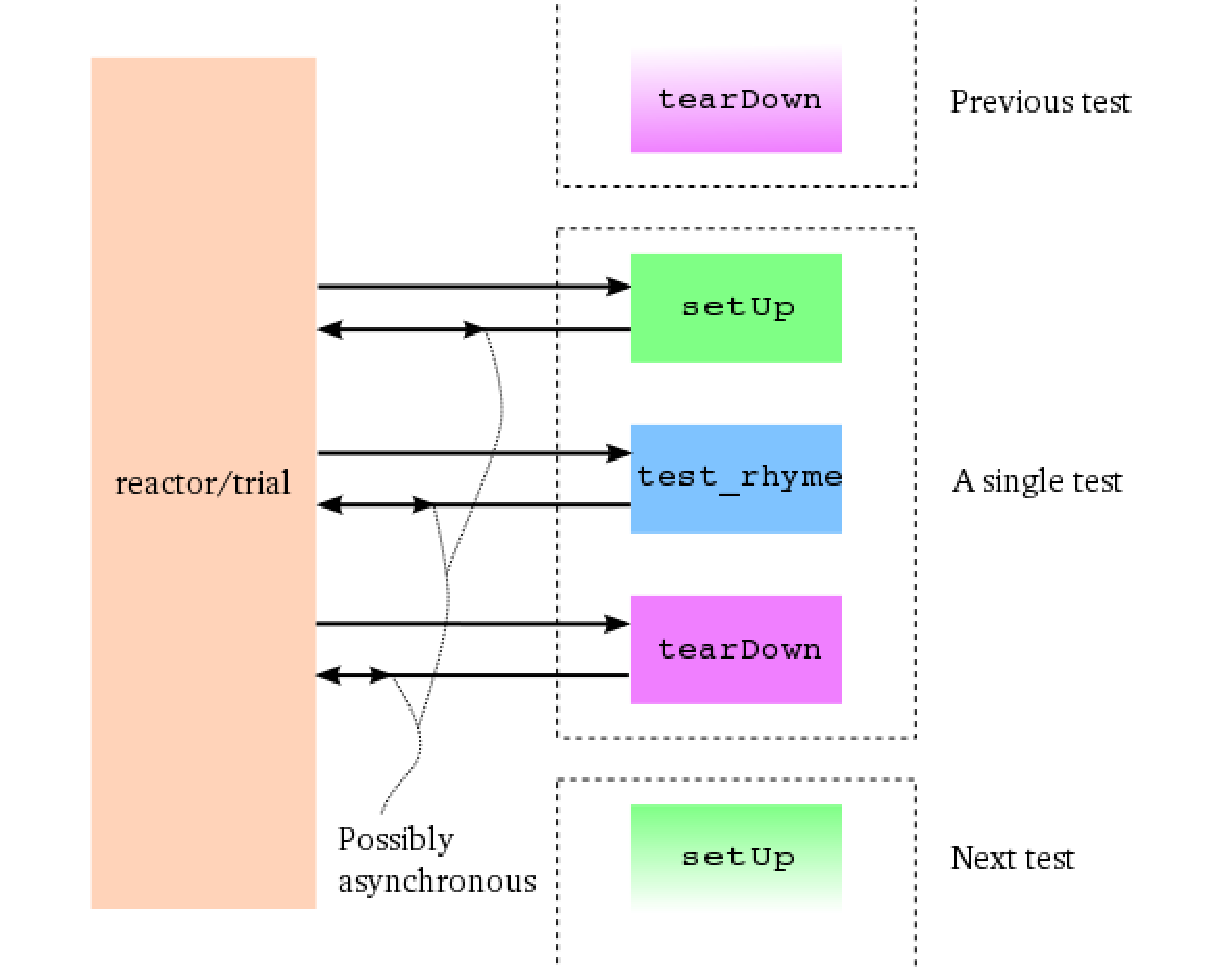
\includegraphics[width=0.8\textwidth]{images/test-1.pdf}
    \caption{Запущенный trial тест\label{fig:test-1}}
\end{center}
\end{figure}


Если вы когда-нибудь использовали подобные системы ранее, 
то вы должны быть знакомы с моделью, за исключением того, что 
все относящиеся к тестам методы могут возвращать deferred'ы.

Система trial - хорошая иллюстрация того как 
``работающая асинхронность'' вызывает изменения во всей программе. 
Для того, чтобы тест (или любая функция) был асинхронным, он должен:

\begin{enumerate}

\item Не блокироваться
\item Зачастую, возвращать deferred

\end{enumerate}


Но это означает, что любые вызовы функции должны 
готовы принять deferred и не блокироваться (
возможно, также возвращать deferred). И так это условие 
распостраняется далее. Таким образом, возникает необходимость в системе, 
подобной trial, которая может управлять асинхронными тестами, которые 
возвращают deferred'ы.

\subsection{Резюме}

Если вы хотите посмотреть больше 
примеров о том как писать unit тесты для кода Twisted, 
вам нужно смотреть не дальше, чем сам Twisted. Twisted 
имеет очень много unit тестов, с новыми добавленными при  
выходе каждого релиза. Поскольку эти тесты изучены 
Twisted экспертами, они являются прекрасным примером того, как 
правильно тестировать Twisted код.


В главе 16 мы будем использовать Twisted для того, чтобы 
сделать наш поэтический сервер подлинным демоном.

\subsection{Упражнения}

\begin{enumerate}

\item Поменяйте один из тестов так, чтобы вызвать ошибку, и 
запустите trial снова, чтобы посмотреть вывод программы.

\item Почитайте \href{http://twistedmatrix.com/documents/current/core/howto/testing.html}{документацию по тестирования в Twisted}\footnote[1]{http://twistedmatrix.com/documents/current/core/howto/testing.html}.

\item Напишите тесты для других поэтических сервисов.

\item Исследуйте \href{http://twistedmatrix.com/trac/browser/trunk/twisted/test}{некоторые тесты} в 
Twisted\footnote{http://twistedmatrix.com/trac/browser/trunk/twisted/test}.

\end{enumerate}

 \clearpage
\clearpage 
% part 16
\section{Демонизация Twisted\label{sec:part16}}

\subsection{Введение}


Серверы, которые мы написали до сих пор, запускались только 
в терминальном окне, с выводом на экран через оператор 
print. Это подходит для программы на стадии разработки, но 
это едва ли подходит для релизов. Хорошо написанная программа, 
готовая для выкладке, должа:

\begin{enumerate}

\item Запускаться как 
\href{http://en.wikipedia.org/wiki/Daemon\_%28computer_software%29}{демон}, отсоединяясь от 
любой терминальной или пользовательской сессии. Сервис 
не должен завершаться после того, как 
администратор отлогился.

\item Отправлять отладочный и ошибочный вывод во 
множество ротируемых лог файлов или в сервис 
\href{http://en.wikipedia.org/wiki/Syslog}{syslog}.

\item Убирать лишние привилегии, например, переключаться к 
к низкопривелигированному пользователю до запуска.

\item Записывать свой 
\href{http://en.wikipedia.org/wiki/Process\_ID}{pid} в файл так, чтобы администратор 
мог без проблем 
\href{http://en.wikipedia.org/wiki/Kill%28%29}{отправить сигналы} в демон.

\end{enumerate}


Мы можем добраться до всех этих вещей, 
используя скрипт twistd, предоставляемый Twisted. Но сначала, 
мы должны быть немного поменять наш код.


\subsection{Концепции}

%Understanding twistd will require learning a few new concepts in Twisted, the most important being a Service. As usual, several of the new concepts are accompanied by new Interfaces.
Для того, чтобы понять twisted, необходимо изучить несколько 
новых понятий в Twisted, наиболее важное из них - Service. Как всегда, 
несколько новых концепций сопровождаются новыми Interface'ми.

\subsubsection{IService}

%The IService interface defines a named service that can be started and stopped. What does the service do? Whatever you like — rather than define the specific function of the service, the interface requires only that it provide a small set of generic attributes and methods.

Интерфейс 
\href{http://twistedmatrix.com/trac/browser/tags/releases/twisted-10.0.0/twisted/application/service.py#L87}{IService} опредлеяет именнованный сервис, 
который может быть запущен и остановлен. 
Интерфейс требует наличия небольшого 
множества основных атрибутов и методов.


Существует два обязательных атрибута: name и running. 
Атрибут name - это просто строка, например 'fastpoetry', или 
None, если вы не хотите давать Вашему сервису название. 
Атрибут running - булево значение, которое устанавливается в true, 
если сервис успешно запущен.


Мы собираемся коснуться лишь некоторых методов IService. 
Мы пропустим некоторые, являющиеся очевидными, и другие, которые 
наиболее продвинуты и в основном не используются в простых 
Twisted программах. Два основных метода IService - 
\href{http://twistedmatrix.com/trac/browser/tags/releases/twisted-10.0.0/twisted/application/service.py#L130}{startService} и 
\href{http://twistedmatrix.com/trac/browser/tags/releases/twisted-10.0.0/twisted/application/service.py#L135}{stopService}:

\begin{scriptsize}\begin{verbatim}
    def startService():
        """
        Start the service.
        """

    def stopService():
        """
        Stop the service.

        @rtype: L{Deferred}
        @return: a L{Deferred} which is triggered when the service has
            finished shutting down. If shutting down is immediate, a
            value can be returned (usually, C{None}).
        """

\end{verbatim}\end{scriptsize}

Что эти методы делают будет зависеть от сервиса. Например, 
метод startService может любое из:

\begin{itemize}
\item Загружать некоторые конфигурационные данные
\item Инициализировать базу данных
\item Начать слушать порт
\item Ничего не делать 
\end{itemize}


Метод stopService может:

\begin{itemize}
\item Сохранять некоторое состояние
\item Закрывать открытие соединения к базе данных
\item Завершать слушать порт
\item Ничего не делать 
\end{itemize}


Когда мы пишем наши пользовательские сервисы, мы должны 
соответсвующе реализовать эти методы. 
Для некоторых общих случаев, подобно прослушиванию порта, 
Twisted предоставляет готовые сервисы, которые мы можем использовать. 


Заметим, что stopService может опционально возвратить deferred, 
который нужно активизировать, когда сервис окончательно 
прекратил работать. Это позволяет нашим сервисам убрать за собой 
до того как приложение завершится. Если Ваш сервис сразу же завершается, 
вы можете возвратить None вместо deferred'а.  


Сервисы могут быть организованы в коллекции, которые вместе  
стартуют и завершаются. Последний метод IService, на который мы будем 
смотреть - 
\href{http://twistedmatrix.com/trac/browser/tags/releases/twisted-10.0.0/twisted/application/service.py#L107}{setServiceParent}, добавляет Service в коллекцию:

\begin{scriptsize}\begin{verbatim}
    def setServiceParent(parent):
        """
        Set the parent of the service.

        @type parent: L{IServiceCollection}
        @raise RuntimeError: Raised if the service already has a parent
            or if the service has a name and the parent already has a child
            by that name.
        """
\end{verbatim}\end{scriptsize}


Любой сервис может иметь родительский, что означает, что 
сервисы могут быть организованы в иерархию. И это подводит нас 
к следующему Interface'у, на который мы собираемся сегодня посмотреть.


\subsubsection{IServiceCollection}

The IServiceCollection interface defines an object which can contain IService objects. A service collection is a just plain container class with methods to:


Интерфейс \href{http://twistedmatrix.com/trac/browser/tags/releases/twisted-10.0.0/twisted/application/service.py#L203}{IServiceCollection} определяет объект, который 
может содержать объекты IService. Коллекция сервисов - просто 
обычный контейнерный класс с методами:

\begin{itemize}

\item Искать сервис по названию (\href{http://twistedmatrix.com/trac/browser/tags/releases/twisted-10.0.0/twisted/application/service.py#L212}{getServiceNamed})

\item Пройтись по всем сервисам в коллекции (\href{http://twistedmatrix.com/trac/browser/tags/releases/twisted-10.0.0/twisted/application/service.py#L222}{\_\_iter\_\_})

\item Добавить сервис в коллекцию (\href{http://twistedmatrix.com/trac/browser/tags/releases/twisted-10.0.0/twisted/application/service.py#L227}{addService})

\item Удалить сервис из коллекции (\href{http://twistedmatrix.com/trac/browser/tags/releases/twisted-10.0.0/twisted/application/service.py#L236}{removeService})

\end{itemize}


Заметим, что реализация IServiceCollection не 
является автоматически реализацией IService, 
но нет препятсвий одному классу реализовать 
оба интерфейса (и мы увидим пример).


\subsubsection{Application}

Twisted Application не определяется отдельным интерфейсом. 
Скорее, объект Application требуется для реализации обоих 
IService и IServiceCollection, также как и для нескольких других, 
которые мы собираемся рассмотреть. 


Приложение - это сервис верхнего уровня, который представляет 
наше полное Twisted приложение. Все другие сервисы в вашем 
демоне будут детьми (или внуками, и т.д.) объекта Application. 


Редко, когда надо реализовывать свое собственное Application. 
Twisted предоставляет реализацию, которую мы будем 
сегодня использовать.

\subsubsection{Twisted логирование}


Twisted включает свое собственную инфраструктуру логирования в модуле 
\href{http://twistedmatrix.com/trac/browser/tags/releases/twisted-10.0.0/twisted/python/log.py}{twisted.python.log}. Основные API для записи в лог простые, поэтому мы просто 
включим небольшой пример, расположенный в 
basic-twisted/log.py, и вы можете просмотреть интересующие Вас детали 
в соответсвующем модуле Twisted.


Мы не будем вам докучать, показывая API для установки логирующих 
обработчиков, поскольку twistd делает это за нас.

\subsection{FastPoetry 2.0}

Хорошо, давайте взглянем на некоторый код. Мы обновили 
наш поэтический сервер для того, чтобы запускать его с 
помощью twistd. Его исходный код расположен в 
\href{http://github.com/jdavisp3/twisted-intro/blob/master/twisted-server-3/fastpoetry.py#L1}{twisted-server-3/fastpoetry.py}. Сначала мы посмотрим на 
\href{http://github.com/jdavisp3/twisted-intro/blob/master/twisted-server-3/fastpoetry.py#L9}{PoetryProtocol}:

\begin{scriptsize}\begin{verbatim}
class PoetryProtocol(Protocol):

    def connectionMade(self):
        poem = self.factory.service.poem
        log.msg('sending %d bytes of poetry to %s'
                % (len(poem), self.transport.getPeer()))
        self.transport.write(poem)
        self.transport.loseConnection()

\end{verbatim}\end{scriptsize}

%Notice instead of using a print statement, we’re using the twisted.python.log.msg function to record each new connection.
Заметьте, что вместо использования оператора print, 
мы используем функцию twisted.python.log.msg для 
записи каждого соединения.
Далее класс \href{http://github.com/jdavisp3/twisted-intro/blob/master/twisted-server-3/fastpoetry.py#L19}{PoetryFactory}:

\begin{scriptsize}\begin{verbatim}
class PoetryFactory(ServerFactory):

    protocol = PoetryProtocol

    def __init__(self, service):
        self.service = service
\end{verbatim}\end{scriptsize}

%As you can see, the poem is no longer stored on the factory, but on a service object referenced by the factory. Notice how the protocol gets the poem from the service via the factory. Finally, here’s the service class itself:

Как вы видите, поэма больше не хранится в PoetryFactory, 
вместо этого она хранится в сервисном объекте, на которую 
есть ссылка из PoetryFactory. Заметьте, как PoetryProtocol получает 
поэму из service через factory. Наконец, далее сам 
\href{http://github.com/jdavisp3/twisted-intro/blob/master/twisted-server-3/fastpoetry.py#L27}{сервисный класс}:

\begin{scriptsize}\begin{verbatim}
class PoetryService(service.Service):

    def __init__(self, poetry_file):
        self.poetry_file = poetry_file

    def startService(self):
        service.Service.startService(self)
        self.poem = open(self.poetry_file).read()
        log.msg('loaded a poem from: %s' % (self.poetry_file,))
\end{verbatim}\end{scriptsize}


Так же как и с другими многочисленными классами Interface, 
Twisted предоставляет базовый класс, который мы можем 
использовать для того, чтобы сделать нашу 
собственную реализацию используя поведение по 
умолчанию. Здесь мы используем класс 
\href{http://twistedmatrix.com/trac/browser/tags/releases/twisted-10.0.0/twisted/application/service.py#L154}{twisted.application.service.Service} для реализации 
нашего PoetryService.


Базовый класс предоставляет реализацию по умолчанию 
всех необходимых методов, поэтому нам нужно 
реализовать только пользовательское поведение. В нашем случае, 
мы просто перегружаем startService для 
загрузки файла с поэзией. Заметим, что мы все равно вызываем 
метод базового класса (который устанавливает для нас 
атрибут running).


Другая сторона здесь плохо упомянута. Объект PoetryService 
не знает ничего о деталях PoetryProtocol. Сервис только 
должен загрузить поэму и обеспечить доступ до него любого 
объекта, который нуждается в поэме. Другими словами, 
PoetryService обеспокоен только высокоуровневыми деталями 
в преоставлении поэзии, а не низкоуровневыми деталями 
отправки по TCP соединению. Таким образом, этот сервисный 
класс мог бы быть использован другим протоколом, скажем UDP или 
XML-RPC. В случае нашего простого сервиса пользы от этого мало, 
но можно представить преимущества в более реалистичной сервисной реализации. 


Если бы это была обычная Twisted программа, весь код, 
на который мы посмотрели до сих пор не был бы в одном файле, 
он был бы в нескольких разных модулях (возможно, 
fastpoetry.protocol и fastpoetry.service). Но, следуя нашей 
обычной практике создания примеров самодостаточными, мы 
включаем все что нам надо в один скрипт.

\subsubsection{Twisted tac файлы}

Оставшийся код в скрипте содержит то, 
что обычно бывает содержимым Twisted tac файла. 
Файл tac - Twisted Application Configuration файл, который 
говорит twistd как создавать приложение. Поскольку это 
конфигурационный файл, то он ответственнен за выбор настроек (подобно 
номерам портов, расположениями файлов с поэзией и т.д.) для 
запуска приложения определенным образом. Другими словами, 
tac файл представляет определенный вид запуска для нашего сервиса (обслужить 
эту поэму на этом порту), а не общий скрипт для 
запуска любого поэтического сервера.


Если бы мы запускали несколько поэтических сервером на одной 
машине, мы бы имели несколько tac файлов для каждого (вот почему 
tac файлы обычно не содержат кода общего назначения). В нашем примере, 
tac файл сконфигурирован для обслуживания poetry/ecstasy.txt на 
порту 10000 loopback интерфейса:

\begin{scriptsize}\begin{verbatim}
# configuration parameters
port = 10000
iface = 'localhost'
poetry_file = 'poetry/ecstasy.txt'
\end{verbatim}\end{scriptsize}


Заметим, что twistd ничего не знает об этих переменных, 
мы их определяем здесь для того, чтобы сохранить все наши 
конфигурационные переменные в одном месте. Фактически, twistd заботится 
только об одной переменной во всем файле, как мы это вскоре поймем. 
Далее мы \href{http://github.com/jdavisp3/twisted-intro/blob/master/twisted-server-3/fastpoetry.py#L44}{начинаем} построение нашего приложения:

\begin{scriptsize}\begin{verbatim}
# this will hold the services that combine to form the poetry server
top_service = service.MultiService()
\end{verbatim}\end{scriptsize}


Наш поэтический сервер состоит из двух 
сервисов: PoetryService, который мы определили выше, и 
встроенный Twisted сервис, который создает слушающий сокет 
нашей поэмы, из которого она будет предоставляться. Поскольку 
эти два сервисы очевидным образом связаны друг с другом, 
мы сгруппируем их вмести, используя \href{http://twistedmatrix.com/trac/browser/tags/releases/twisted-10.0.0/twisted/application/service.py#L253}{MultiService} - класс Twisted, 
который реализует IService вместе с IServiceCollection.


Будучи сервисной коллекцией, MultiService сгруппирует 
наши два поэтических сервиса вместе. И будучи сервисом, 
MultiService запустит оба дочерних сервиса, когда 
MultiService сам запустится, и остановит их, когда сам остановится. 
Давайте добавим наш первый поэтический сервис в коллекцию:

\begin{scriptsize}\begin{verbatim}
# the poetry service holds the poem. it will load the poem when it is
# started
poetry_service = PoetryService(poetry_file)
poetry_service.setServiceParent(top_service)
\end{verbatim}\end{scriptsize}


Эта достаточно удобная вещь. Мы только создаем 
PoetryService и затем добавляем его в коллекцию, 
используя setServiceParent, который унаследован из 
базового класса Twisted. Затем мы \href{http://github.com/jdavisp3/twisted-intro/blob/master/twisted-server-3/fastpoetry.py#L53}{слушаем} TCP сокет:

\begin{scriptsize}\begin{verbatim}
# the tcp service connects the factory to a listening socket. it will
# create the listening socket when it is started
factory = PoetryFactory(poetry_service)
tcp_service = internet.TCPServer(port, factory, interface=iface)
tcp_service.setServiceParent(top_service)
\end{verbatim}\end{scriptsize}


Twisted предоставляет сервис TCPServer для создания 
слушающего TCP сокета, присоединенного к 
произвольной factory (в нашем случае - PoetryFactory). 
Мы не вызываем reactor.listenTCP напрямую, поскольку 
работа tac файла - сделать наше приложение готовым к старту 
не запуская его. TCPServer создаст сокет после того, как 
он запустится скриптом twistd.  


Вы могли заметить, что мы не беспокоились заданием 
названия сервиса. Именование сервисов не является 
обязательным, а наоборот - опциональным свойством, 
которое вы можете использовать, если хотите 
<<просматривать>> сервисы во время запуска. Поскольку 
нам не нужно этого делать в нашем маленьком приложении, 
то мы не беспокоимся об этом.


Хорошо, мы получили оба наших сервиса, объединенных 
в коллекцию. Теперь мы только сделаем Application и 
добавим нашу коллекцию в него:

\begin{scriptsize}\begin{verbatim}
# this variable has to be named 'application'
application = service.Application("fastpoetry")

# this hooks the collection we made to the application
top_service.setServiceParent(application)
\end{verbatim}\end{scriptsize}


Единственная переменная в этом скрипте, которая 
интересует twistd - переменная application. Это то, как 
twistd найдет приложение, которое предполагается запустить (поэтому 
переменная должна иметь название "application"). И когда 
приложение запустится, все сервисы, которые мы туда добавили, 
также будут запущены.


На рисунке \ref{fig:application} показана структура приложения, 
которое мы только что построили:

\begin{figure}[h]
\begin{center}
    \includegraphics[width=0.5\textwidth]{images/application.pdf}
    \caption{Структура fastpoetry приложения\label{fig:application}}
\end{center}
\end{figure}


\subsubsection{Запуск сервера}


Давайте запустим наш сервер. 
Поскольку наш скрипт - tac файл, то нам нужно запустить его с помощью twistd.  
Конечно же, tac файлы - обычные Python скрипты. 
Давайте сначала запустим tac файл без twistd, 
просто используя интерпретатор Python и посмотрим, что получается:

\begin{scriptsize}\begin{verbatim}
python twisted-server-3/fastpoetry.py
\end{verbatim}\end{scriptsize}


Если вы сделаете это, вы обнаружите, что ничего не произошло! 
Как мы говорили до этого, работа tac файла - сделать приложение 
готовым для запуска, без его запуска. В качестве напоминание об этом 
специальном назначении tac файлов, некоторые люди называют их с 
расширением .tac вместо .py. Скрипт twistd не заботится о 
расширении файла.


Давайте запустим наш сервер по-настоящему, используя twistd:

\begin{scriptsize}\begin{verbatim}
twistd --nodaemon --python twisted-server-3/fastpoetry.py
\end{verbatim}\end{scriptsize}


После запуска такой команды вы увидите похожий вывод:

\begin{scriptsize}\begin{verbatim}
2010-06-23 20:57:14-0700 [-] Log opened.
2010-06-23 20:57:14-0700 [-] twistd 10.0.0 (/usr/bin/python 2.6.5) starting up.
2010-06-23 20:57:14-0700 [-] reactor class: twisted.internet.selectreactor.SelectReactor.
2010-06-23 20:57:14-0700 [-] __builtin__.PoetryFactory starting on 10000
2010-06-23 20:57:14-0700 [-] Starting factory <__builtin__.PoetryFactory instance at 0x14ae8c0>
2010-06-23 20:57:14-0700 [-] loaded a poem from: poetry/ecstasy.txt
\end{verbatim}\end{scriptsize}

Здесь нужно отметить несколько вещей:

\begin{enumerate}

\item вы видите вывод системы логирования Twisted, в том числе вызов 
log.msg в PoetryFactory. Но мы не устанавливали logger в нашем tac 
файле, так как twistd должен это сделать для нас.  

\item вы также можете увидеть, что наши два основных сервиса, PoetryService и TCPServer,
запустились.

\item Командная строка не возвращается. Это означает, что наш сервер 
не запущен как демон. По умолчанию, twistd запускает сервер как демон (это 
основная причина существования twistd), но если вы используете опцию 
--nodaemon, то twistd запустит ваш сервер как обычный консольный процесс, и 
лог будет выводится на стандартный вывод. Это полезно при отладки ваших 
tac файлов.

\end{enumerate}


Теперь протестируем сервер путем скачивания поэмы одним из 
наших поэтических клиентов или даже netcat'м:

\begin{scriptsize}\begin{verbatim}
netcat localhost 10000
\end{verbatim}\end{scriptsize}

Такая команда должна скачать поэму из сервера, и вы 
увидите новую запись в логе подобную такой: 

\begin{scriptsize}\begin{verbatim}
2010-06-27 22:17:39-0700 [__builtin__.PoetryFactory] sending 3003 bytes of poetry to IPv4Address(TCP, '127.0.0.1', 58208)
\end{verbatim}\end{scriptsize}


Эта запись появляется в результате вызова log.msg в 
PoetryProtocol.connectionMade. Если вы сделаете еще запросы к 
серверу, то на каждый запрос вы увидите новую запись в логе.


Теперь остановим сервер, нажав Ctrl-C. вы должны увидеть строки подобные:

\begin{scriptsize}\begin{verbatim}
^C2010-06-29 21:32:59-0700 [-] Received SIGINT, shutting down.
2010-06-29 21:32:59-0700 [-] (Port 10000 Closed)
2010-06-29 21:32:59-0700 [-] Stopping factory <__builtin__.PoetryFactory instance at 0x28d38c0>
2010-06-29 21:32:59-0700 [-] Main loop terminated.
2010-06-29 21:32:59-0700 [-] Server Shut Down.
\end{verbatim}\end{scriptsize}


Как вы видите, Twisted не просто разрушается, а завершает сам 
себя чисто и говорит вам о завершении в логе. Заметим, что два 
наших основных сервис также сами себя завершают.


Хорошо, теперь запустим сервер еще раз:

\begin{scriptsize}\begin{verbatim}
twistd --nodaemon --python twisted-server-3/fastpoetry.py
\end{verbatim}\end{scriptsize}


Откройте другую консоль и зайдите в директорию twisted-intro. 
В директории должен появится файл twistd.pid. Этот файл создан 
twistd и содержит идентификатор процесса нашего запущенного 
сервера. Попробуйте запустить эту команду для завершения сервера: 

\begin{scriptsize}\begin{verbatim}
kill `cat twistd.pid`
\end{verbatim}\end{scriptsize}

Заметьте, что twistd стирает файл с pid'м, когда наш сервис завершается.


\subsubsection{Реальный демон}


Теперь давайте запустим наш сервер как 
демон, который даже проще сделать, поскольку 
по умолчанию twistd демонизирует процесс:

\begin{scriptsize}\begin{verbatim}
twistd --python twisted-server-3/fastpoetry.py
\end{verbatim}\end{scriptsize}


На этот раз мы сразу же получаем командную строку обратно. 
Если вы посмотрите на содержимое вашей директории, 
то в дополнение к файлу twistd.pid, созданное для сервера, 
который мы только что запустили, вы увидите файл с 
логами --- twistd.log, который отображает тоже самое, что и 
ранее отображалось в консоли.


При запуске демона, twistd устанавливает обработчик логов, 
который пишет в файл вместо стандартного вывода. Лог-файл 
по умолчанию --- это twistd.log, расположенный в той же 
директории, где вы запустили twistd, но, если вы хотите, то 
можете менять файл использованием опции \textit{\symbol{45}\symbol{45}logfile}. 
Обработчик, который устанавливает twistd также ротирует лог, 
когда размер превышает один мегабайт.


Вы можете увидеть запущенный сервер, просмотрев список 
всех процессов в вашей системе. Продолжим и проверим 
сервер, скачав еще одну поэму. Вы увидите новые записи 
в лог файле для каждого запроса на скачивание поэмы.


Поскольку сервер больше не присоединен к консоли (и 
другим процессам, кроме init), вы не можете завершить его 
нажав Ctrl-C. Как реальный демон, процесс продолжит работу, 
даже если вы отлогинетесь. Но мы все еще можем использовать 
файл twistd.pid, чтобы остановить процесс:

\begin{scriptsize}\begin{verbatim}
kill `cat twistd.pid`
\end{verbatim}\end{scriptsize}


И когда это происходит, то в логе появляются 
сообщения об остановке сервера, файл twistd.pid 
удаляется, и наш сервер завершается.


Это хорошая идея проверить другие опции twistd. 
Например, вы можете сказать twistd переключиться на 
другого пользователя или группу до запуска демона (это 
типичный случай понижения привелегий Вашего сервера, 
которые ему не нужны, в качестве меры предосторожности). 
Мы не будем беспокоиться тщательным изучением этих 
дополнительных опций, вы можете найти их, используя 
опцию --help. 


\subsection{Системы плагинов в Twisted}

Хорошо, теперь мы можем использовать twistd для запуска 
наших серверов как подлинных демонов. Это все очень 
здорово, и тот факт, что наш ``конфигурационные'' файлы 
являются реально файлами с исходниками на Python'е, дает 
нам огромную гибкость во многих вещах. Но, нам не всегда 
нужно так много гибкости. Для наших поэтических серверов, 
обычно мы заботимся только о нескольких опциях:

\begin{enumerate}
\item Поэма для обслуживания
\item Порт для обслуживания поэмы
\item Интерфейс для прослушивания
\end{enumerate}


Создавать новые tac файлы с простыми изменениями 
переменных кажется чрезмерным. Система плагинов в 
Twisted позволяет нам сделать тоже самое.


Twisted плагины предоставляют способ 
определения именованных приложений с 
пользовательскими опциями, которые 
twistd может автоматически распознать и 
запустить. Twisted сам построен из 
множества встроенных плагинов. вы можете 
их увидеть, запуская twisted без аргументов. Попробуйте 
запустить сейчас вне директории twisted-intro. 
После раздела с помощью, вы увидите вывод подобный:

\begin{scriptsize}\begin{verbatim}
    ...
    ftp                An FTP server.
    telnet             A simple, telnet-based remote debugging service.
    socks              A SOCKSv4 proxy service.
    ...
\end{verbatim}\end{scriptsize}


Каждая строка показывает один из встроенных плагинов из Twisted. 
И вы можете любой из них, используя twistd.


Каждый плагин также имеет свое множество опций, которые вы 
можете изучить, используя опицию --help. Давайте посмотрим, 
какие опции имеет плагин ftp:

\begin{scriptsize}\begin{verbatim}
twistd ftp --help
\end{verbatim}\end{scriptsize}

Заметим, что нужно поместить опцию --help после команды 
ftp, поскольку вам нужны опции ftp, а не опции twistd.
вы можете запустить ftp сервер с помощью twistd также, 
как мы запускали наш поэтический сервер. Но, поскольку это 
плагин, то мы запускаем его по его названию:

\begin{scriptsize}\begin{verbatim}
twistd --nodaemon ftp --port 10001
\end{verbatim}\end{scriptsize}


Эта команда запускает ftp плагин в недемонизированном виде 
на порту 10001. Заметим, что опция twistd 
\textit{\symbol{45}\symbol{45}nodaemon} помещается 
до названия плагины, в то время как опции, специфичные для плагина, 
помещаются после его названия. Так же как и наш поэтический 
сервер, вы можете остановить плагин с помощью Ctrl-C.


Ok, давайте превратим наш поэтический сервер в Twisted 
плагин. Но сначала, нам нужно осознать несколько 
новый концепций.

\subsubsection{IPlugin}

Любой Twisted плагин должен реализовывать интерфейс 
\href{http://twistedmatrix.com/trac/browser/tags/releases/twisted-10.0.0/twisted/plugin.py#L38}{twisted.plugin.IPlugin}. 
Если вы посмотрите на его объявление, то  
вы обнаружите, что он в действительности не определяет никакие методы. 
Реализация IPlugin - просто способ для плагина, сказать ``Привет, я - плагин!'' 
так, чтобы twistd мог найти его. Конечно же, чтобы его можно было использовать,  
он должен реализовать некоторый другой интерфейс, и мы вскоре 
до этого доберемся.


Но, как узнать, дейcтвительно ли объект реализует пустой интерфейс? 
Пакет zope.interface имеет функцию, которая позволяет указать то, что 
определенный класс реализует определенный интерфейс. Мы рассмотрим пример 
использования этой функции в plugin-версии нашего поэтического сервера. 


\subsubsection{IServiceMaker}

В дополнение к IPlugin, наш плагин будет реализовывать 
интерфейс \href{http://twistedmatrix.com/trac/browser/tags/releases/twisted-10.0.0/twisted/application/service.py#L25}{IServiceMaker}. Объект, который реализует IServiceMaker, знает 
как создавать IService, который будет формировать основной элемент 
запуска application. IServiceMaker определяет три атрибута и метод:

\begin{enumerate}
\item tapname: строка с названием нашего плагина. Аббревиатура ``tap'' 
означает Twisted Application Plugin. Заметим, что более старые версии Twisted 
также использовали pickled application files, называемые ``tapfiles'', но это функциональность 
устарела.
\item description: описание плагина, который twistd будет отображать как часть своего help текста.
\item options: объект, который описывает опции командной строки, которые принимает плагин.
\item makeService: метод, который создает новый объект IService 
по заданному множеству опций командной строки.

\end{enumerate}

Мы увидим то, как все это соединяется вместе в следующей версии нашего 
поэтического сервера.


\subsection{Fast Poetry 3.0}

Теперь мы готовы посмотреть на плагин версию Fast Poetry, 
расположенную в  
\href{http://github.com/jdavisp3/twisted-intro/blob/master/twisted/plugins/fastpoetry\_plugin.py#L1}{twisted/plugins/fastpoetry\_plugin.py}.


Как вы могли заметить, название директорий отличается от других 
примеров. Это потому что twistd требует, чтобы плагин файлы 
были расположены в директории twisted/plugins (вам не нужно 
создавать никаких \_\_init\_\_.py файлов); вы можете иметь 
несколько директорий twisted/plugins в PYTHONPATH, 
и twisted все их найдет. Название файла, которое вы используете 
для плагина, не имеет значения, но все таки хорошая идея 
именовать его согласно тому приложению, которое он представляет, 
подобно тому как мы это сделали.


Первая часть нашего плагина состоит из тех же 
protocol, factory и service реализаций, как и наш 
tac файл. И так же как и раньше, этот код обычно находится 
в разных модулях, но мы поместим его в плагин, для того, чтобы 
сделать пример самодостаточным.


Далее идет объявление комнадных опций плагина:

\begin{scriptsize}\begin{verbatim}
class Options(usage.Options):

    optParameters = [
        ['port', 'p', 10000, 'The port number to listen on.'],
        ['poem', None, None, 'The file containing the poem.'],
        ['iface', None, 'localhost', 'The interface to listen on.'],
        ]
\end{verbatim}\end{scriptsize}


Этот код определяет опции, специфичные для плагина, которые 
пользователь может поместить после названия 
плагина при использовании twistd. Мы не будем вдаваться в 
подробности, так как тут все достаточно понятно. Теперь, мы 
перейдем к основной части нашего плагина - классу PoetryServiceMaker: 


\begin{scriptsize}\begin{verbatim}
class PoetryServiceMaker(object):

    implements(service.IServiceMaker, IPlugin)

    tapname = "fastpoetry"
    description = "A fast poetry service."
    options = Options

    def makeService(self, options):
        top_service = service.MultiService()

        poetry_service = PoetryService(options['poem'])
        poetry_service.setServiceParent(top_service)

        factory = PoetryFactory(poetry_service)
        tcp_service = internet.TCPServer(int(options['port']), factory,
                                         interface=options['iface'])
        tcp_service.setServiceParent(top_service)

        return top_service
\end{verbatim}\end{scriptsize}


Здесь вы видите как функция zope.interface.implements используется для 
объявления того, что наш класс реализует оба IServiceMaker и IPlugin. 
На этот раз, нам не нужно создавать объект Application, мы только 
создаем и возвращаем сервис более высокого уровня, который запустит наш 
application, и twistd позаботится обо всем остальном. Заметим то, как мы 
используем аргумент options для того, чтобы получить опции 
командной строки, специфичные для плагина, переданные twistd.


После объявления класса, осталась только одна вещь, которую надо 
сделать:

\begin{scriptsize}\begin{verbatim}
service_maker = PoetryServiceMaker()
\end{verbatim}\end{scriptsize}


Скрипт twistd обнаружит экземпляр нашего плагина и использует 
его для создания сервиса высокого уровня. В отличие от tac файла, 
переменная name, которую мы выбираем, неважна. Важно, что наш 
объект реализует оба IPlugin и IServiceMaker.  


Посколе того, как мы создали наш плагин, давайте запустим его. 
Убедитесь, что вы находитесь в директории twisted-intro или, что
эта директория находится в PYTHONPATH. Затем, попробуйте 
запустить twistd. вы должны увидеть, что ``fastpoetry'' в списке 
плагинов вместе с описанием из нашего файла с плагином.


Вы также заметите, что создался новый файл dropin.cache в 
директории twisted/plugins. Этот файл создается twistd для 
ускорения последующих поисков плагинов.


Теперь давайте получим некоторую помощь по использованию 
нашего плагина:

\begin{scriptsize}\begin{verbatim}
twistd fastpoetry --help
\end{verbatim}\end{scriptsize}


Вы увидите опции, специфичные для плагина fastpoetry в тексте 
помощи. И наконец, давайте запустим наш плагин:

\begin{scriptsize}\begin{verbatim}
twistd fastpoetry --port 10000 --poem poetry/ecstasy.txt
\end{verbatim}\end{scriptsize}


Эта команда запустит сервер fastpoetry как демон. 
Как и раньше,  вы увидите оба файла twistd.pid и 
twistd.log в текущей директории. После тестирования 
нашего сервера, вы можете остановить его:

\begin{scriptsize}\begin{verbatim}
kill `cat twistd.pid`
\end{verbatim}\end{scriptsize}

Вот как создавать Twisted плагины.


\subsection{Резюме}

В этой главе мы изучили то, как превращать 
Twisted сервера в долгоживущие демоны. Мы 
затронули систему логирования Twisted и как 
использовать twistd для запуска Twisted приложений 
ввиде демонизированных процессов, 
как создавать tac конфигурационные файлы,
как создавать и запускать Twisted плагины. 
В главе \ref{sec:part17} мы возвратимся к более фундаментальной 
теме асинхронного программирования и посмотрим 
на другой способ структурирования наших callback'в 
в Twisted. 


\subsection{Упражнения}

\begin{enumerate}

\item Поменяйте tac файл для обслуживания второй поэмы на другом 
порту. Сохраните сервисы для каждой поэмы отдельно, используя другой 
объект MultiService.

\item Создайте новый tac файл, который запустит поэтический прокси 
сервер.

\item Модифицируйте файл plugin для того, чтобы он принимал 
необязательный второй поэтический файл и второй порт, для 
обслуживания.

\item Создайте новый плагин для поэтического прокси сервера.

\end{enumerate}




 \clearpage
\clearpage 
% part 17
\section{Еще один способ написания callback'в\label{sec:part17}}

\subsection{Введение}


В этой главе мы возвратимся к предмету callback'в. Мы изучим 
еще одну технику написания callback'в в Twisted, которая использует 
генераторы. Мы покажем как эта техника работает и сравним с использованием 
<<чистыx>> Deferred'ов. Наконец, мы перепишем один из наших поэтических 
клиентов, используя эту технику. Но сначала, давайте посмотрим на то, 
как работают генераторы, чтобы мы могли увидеть, почему они 
являются кандидатами для создания callback'в.

\subsubsection{Краткий обзор генераторов}

Как вы вероятно знаете, генератор в Python'е - это 
``перезапускаемая функция'', которую вы создаете 
используя выражение yield в ее теле. 
Делая так, функция становится ``генераторной функцией'', 
которая возвращает итератор, который вы можете использовать 
для запуска функции как серии шагов. Каждый цикл 
итератора перезапускает функцию, которая 
продолжает выполняться до тех пор пока не достигнет 
следующего вызова yield.


Генераторы (и итераторы) зачастую используются для представления 
лениво созданных последовательностей значений. Давайте посмотрим 
на пример кода в inline-callbacks/gen-1.py:

 \begin{verbatim}
def my_generator():
    print 'starting up'
    yield 1
    print "workin'"
    yield 2
    print "still workin'"
    yield 3
    print 'done'

for n in my_generator():
    print n
\end{verbatim} 


Здесь мы имеем генератор, который создает последовательность 
1, 2, 3. Если вы запустите этот код, то вы увидите, что операторы print в 
генераторе, чередуются с оператором print в цикле, 
проходящему по генератору.


Вы можете сделать этот код более явным 
путем создания самого генератора (inline-callbacks/gen-2.py):

 \begin{verbatim}
def my_generator():
    print 'starting up'
    yield 1
    print "workin'"
    yield 2
    print "still workin'"
    yield 3
    print 'done'

gen = my_generator()

while True:
    try:
        n = gen.next()
    except StopIteration:
        break
    else:
        print n
\end{verbatim} 


Генератор --- это просто объект для получения последовательных значений. 
Мы также можем рассмотреть вещи с точки зрения самого генератора:

\begin{enumerate}
\item Функция-генератор не начинает запуск до тех пор, пока она не 
будет вызвана циклом (используя метод next).
\item Запущенный генератор продолжает выполняться до тех пор, пока 
он не возвращается циклу (используя yield). 
\item Когда цикл запускает другой код (подобный оператору print в примере), 
генератор не выполняется.
\item Когда генератор выполняется, цикл не выполняется (блокируется, ожидая возврата генератора).
\item Когда генератор уступает контроль циклу, может пройти произвольное 
количество времени (может быть выполнено произвольное количество кода) до того, 
как генератор запустится снова.
\end{enumerate}


Это очень похоже на то, как работают callback'и в асинхронной системе. 
Мы можем представить, что цикл while - reactor, а 
генератор - серия callback'в, разделенных операторами yield, 
с интересным фактом, что все callback'и разделяют одно и то же 
локальное пространство переменных, и пространство имен сохраняется 
от между всеми вызовами callback'в.


Кроме того, вы можете иметь несколько одновременно активных генераторов 
(посмотрите пример в inline-callbacks/gen-3.py), 
с их чередующимися ``callback'ми'', 
также как вы можете иметь независимые асинхронные задачи, 
запущенные в системе, подобной Twisted.


Хотя, что-то еще пропущено. Callback'и не только вызываются реактором, 
они также получают информацию. Как часть цепочки deferred'а, callback 
либо получает результат, в форме одного Python значения, либо ошибку в 
форме объекта типа Failure. 


Начиная с Python 2.5, функциональность генераторов была 
расширена, что позволило отправлять информацию 
генератору, когда он перезапускается; пример 
inline-callbacks/gen-4.py иллюстрирует это свойство:


 \begin{verbatim}
class Malfunction(Exception):
    pass

def my_generator():
    print 'starting up'

    val = yield 1
    print 'got:', val

    val = yield 2
    print 'got:', val

    try:
        yield 3
    except Malfunction:
        print 'malfunction!'

    yield 4

    print 'done'

gen = my_generator()

print gen.next() # start the generator
print gen.send(10) # send the value 10
print gen.send(20) # send the value 20
print gen.throw(Malfunction()) # raise an exception inside the generator

try:
    gen.next()
except StopIteration:
    pass
\end{verbatim} 


В Python 2.5 и выше, оператор yield - выражение, 
которое возвращает значение. А код, который перезапускает генератор, 
может установить это значение, используя метод send вместо next (если 
вы используете next, то значение - None). Более того, 
вы можете генерировать произвольное 
исключение внутри генератора, используя метод throw. И это круто.


\subsection{Встроенные callback'и}

%Given what we just reviewed about sending and throwing values and exceptions into a generator, we can envision a generator as a series of callbacks, like the ones in a deferred, which receive either results or failures. The callbacks are separated by yields and the value of each yield expression is the result for the next callback (or the yield raises an exception and that’s the failure). Figure 35 shows the correspondence:

Взяв за основу то, что мы только что просмотрели об отправке значений и 
генерировании исключений в генераторе, мы можем представить генератор 
как серию callback'в, подобных callback'ам в deferred'е, которые 
получают либо результаты, либо ошибки. callback'и разделены 
yield'ми и значения каждого yield выражения - результат для следующего 
callback'а (или yield генерирует исключение в случае ошибки). 
На рисунке \ref{fig:generator-callbacks1} показано соответствие:
 
% fig35
\begin{figure}[h]
\begin{center}
    \includegraphics[width=0.5\textwidth]{images/generator-callbacks1.pdf}
    \caption{Генератор как последовательность callback'в\label{fig:generator-callbacks1}}
\end{center}
\end{figure}


Когда серия callback'в соединена вместе в deferred, 
каждый callback получает результат из предыдущего. Это достаточно 
просто сделать и с генератором - просто отправить значение, которое 
имеется от предыдущего запуска генератора, в следующий раз, когда 
вы перезапускаете его. Это кажется немного глупо. Поскольку генератор 
вычислил значение, почему нужно заботится об отправке его назад? 
Генератор может просто сохранить значение в переменной до 
следующего раза, когда она понадобится. Так какой в этом смысл?


Вспомним факт, который мы изучили в главе 13, когда 
callback'и в deferred'е могли возвращать deferred'ы. 
И когда такое происходило, внешний deferred останавливался до тех 
пор, пока внутренный deferred активизировался, и затем 
следующий callback (или errback) в цепочке внешнего deferred'а 
вызывался с результатом (или ошибкой) из внутреннего deferred'а.


Представим, что наш генератор производит объект deferred вместо 
обычного Python значения. Генератор приостановится и это происходит 
автоматически; генераторы всегда приостанавливаются после каждого 
оператора yield до тех пор, пока они явно не перезапустятся. 
Таким образом мы можем приостановить перезапуск генератора до тех пор, 
пока deferred активизируется, в этот момент мы либо отправляем значение 
(если deferred завершился успешно), либо генерируем исключение (если 
deferred завершился с ошибкой). Это могло бы сделать наш генератор 
подлинной последовательностью асинхронных callback'в, что  
являетcя основной идеей в реализации функции inlineCallbacks в twisted.internet.defer. 


\subsubsection{inlineCallbacks}

Рассмотрим теперь пример inline-callbacks/inline-callbacks-1.py:

 \begin{verbatim}
from twisted.internet.defer import inlineCallbacks, Deferred

@inlineCallbacks
def my_callbacks():
    from twisted.internet import reactor

    print 'first callback'
    result = yield 1 # yielded values that aren't deferred come right back

    print 'second callback got', result
    d = Deferred()
    reactor.callLater(5, d.callback, 2)
    result = yield d # yielded deferreds will pause the generator

    print 'third callback got', result # the result of the deferred

    d = Deferred()
    reactor.callLater(5, d.errback, Exception(3))

    try:
        yield d
    except Exception, e:
        result = e

    print 'fourth callback got', repr(result) # the exception from the deferred

    reactor.stop()

from twisted.internet import reactor
reactor.callWhenRunning(my_callbacks)
reactor.run()
\end{verbatim} 


Запустите пример, и вы увидите выполнение генератора, 
который по завершению останавливает reactor. Пример иллюстрирует 
несколько свойств функции inlineCallbacks.


Во-первых, 
inlineCallbacks - декоратор, и он всегда декорирует 
генераторные функции, то есть функции, которые используют 
yield. Основная цель inlineCallbacks - превратить генератор 
в серию асинхронных callback'в, согласно тому, как мы 
обсуждали это ранее.


Во-вторых, когда мы вызываем декоратор inlineCallbacks, то 
нам не нужно самим вызывать методы next, send или throw. 
Декоратор сам вызывает эти методы и 
гарантирует, что генератор выполнит весь код (предполагая, 
что в нем не произошло исключения). 


В-третьих, если в генераторе порождается значение, не являющееся 
deferred'ом, то генератор сразу же возвратит себе управление, и 
yield вернет это значение. 


И наконец, если мы порождаем deferred из генератора, 
то генератор не получит управления обратно до тех пор, пока 
deferred не активизируется. После успешного завершения deferred'а, 
управление отдается обратно к генератору, и yield возвращает 
то, что возвратил завершившийся deferred. Eсли 
deferred завершается с ошибкой, то оператор yield генерирует 
исключение. Заметим, что исключение - это просто обычный 
Exception объект, а не объект типа Failure, и мы можем 
поймать его с помощью оператора try/except, обернутого вокруг yield.


В примере мы использовали callLater для активизации  
deferred'в после короткого периода времени. Это удобный 
способ установить неблокирующую задержку в нашу callback 
цепочку, в реальных более сложных програмах, 
мы бы порождали deffered, возвращенный 
некоторой другой асинхронной операцией (например, get\_poetry), 
вызванной из нашего генератора.


Хорошо, теперь мы знаем как запускать функции с декоратором inlineCallbacks, 
но какое значение возвратит 'yield 1'? Ответ - deferred. 
Поскольку мы не можем точно знать, 
когда генератор остановится (он может породить один или 
несколько deferred'ов), декорированная функция сама асинхронная и 
deferred является подходящим возвращяемым значением. 

%Ok, now we know how an inlineCallbacks-decorated function runs, but what return value do you get if you actually call one? As you might have guessed, you get a deferred. Since we can’t know exactly when that generator will stop running (it might yield one or more deferreds), the decorated function itself is asynchronous and a deferred is the appropriate return value. Note the deferred that is returned isn’t one of the deferreds the generator may yield. Rather, it’s a deferred that fires only after the generator has completely finished (or throws an exception).

Поскольку мы заранее не можем сказать, когда 
завершится выполнение генератора, так как он 
может породить несколько deferred'ов, то 
декоратор inlineCallbacks - асинхронная функция 
и deferred - самое подходящее значение в качестве 
возвращаемого значения yield. Заметим, что для возвращаемого  
deferred'а, генератор не может вызвать yield. Заметим, что 
возвращаемый генератором deferred не порождается оператором yield. 
Напротив, этот deferred может активизироваться только после того как 
генератор полностью завершился (или выкинул исключенение). 

%If the generator throws an exception, the returned deferred will fire its errback chain with that exception wrapped in a Failure. But if we want the generator to return a normal value, we must “return” it using the defer.returnValue function. Like the ordinary return statement, it will also stop the generator (it actually raises a special exception). The inline-callbacks/inline-callbacks-2.py example illustrates both possibilities.

Если генератор выкидывает исключение, 
то возвращаемый deferred активизирует свою 
цепочку errback с исключением, обернутым в Failure. 
Но, если вы хотите, чтобы генератор возвращал 
обычное значение, вы должны использовать функцию 
defer.returnValue. Подобно обычному оператору return, 
он также остановит генератор (в действительности, он 
генерирует специальное исключение). Пример 
\href{http://github.com/jdavisp3/twisted-intro/blob/master/inline-callbacks/inline-callbacks-2.py#L1}{inline-callbacks/inline-callbacks-2.py} иллюстрирует 
обе возможности.

\subsection{Клиент 7.0}

Давайте включим inlineCallbacks в новую версию нашего поэтического 
клиента. Код находится в twisted-client-7/get-poetry.py. 
Можно сравнить с кодом клиента 6.0 в twisted-client-6/get-poetry.py. 
Изменения в основном коснулись poetry\_main:

 \begin{verbatim}
def poetry_main():
    addresses = parse_args()

    xform_addr = addresses.pop(0)

    proxy = TransformProxy(*xform_addr)

    from twisted.internet import reactor

    results = []

    @defer.inlineCallbacks
    def get_transformed_poem(host, port):
        try:
            poem = yield get_poetry(host, port)
        except Exception, e:
            print >>sys.stderr, 'The poem download failed:', e
            raise

        try:
            poem = yield proxy.xform('cummingsify', poem)
        except Exception:
            print >>sys.stderr, 'Cummingsify failed!'

        defer.returnValue(poem)

    def got_poem(poem):
        print poem

    def poem_done(_):
        results.append(_)
        if len(results) == len(addresses):
            reactor.stop()

    for address in addresses:
        host, port = address
        d = get_transformed_poem(host, port)
        d.addCallbacks(got_poem)
        d.addBoth(poem_done)

    reactor.run()
\end{verbatim} 


В новой версии генератор get\_transformed\_poem с декоратором 
inlineCallbacks отвечают за скачивание поэмы и ее 
преобразование (через трасформирующий сервер). Поскольку 
обе операции асинхронные, мы порождаем (оператором yield) 
deferred и затем явно ждем результат. Так же как и клиент 6.0, 
если преобразование завершилось с ошибкой, то поэма не 
меняется. Заметим, что мы можем использовать операторы 
try/except для управления асинхронными ошибками внутри 
генератора.


Мы можем проверить новый клиент так же как и раньше. 
Сначала запустим трансформирующий сервер:

 \begin{verbatim}
python twisted-server-1/tranformedpoetry.py --port 10001
\end{verbatim} 

Затем запустим несколько поэтических серверов:

 \begin{verbatim}
python twisted-server-1/fastpoetry.py --port 10002 poetry/fascination.txt
python twisted-server-1/fastpoetry.py --port 10003 poetry/science.txt
\end{verbatim} 

Теперь можно запустить новый клиент:

 \begin{verbatim}
python twisted-client-7/get-poetry.py 10001 10002 10003
\end{verbatim} 

Попробуйте отключить один или несколько серверов, для 
того, чтобы посмотреть как клиент управляет ошибками.


\subsection{Обсуждение}

Подобно объекту Deferred, функция inlineCallbacks дает 
новый способ организации наших асинхронных callback'в. 
Так же как и с deferred'ми, inlineCallbacks не меняет 
правила игры. Наши callback'и запускаются 
один за раз и вызываются реактором. Мы можем убедиться 
в этом, распечатав traceback из внутреннего callback'а, 
так, как это сделано в примере 
\href{http://github.com/jdavisp3/twisted-intro/blob/master/inline-callbacks/inline-callbacks-tb.py#L1}{inline-callbacks/inline-callbacks-tb.py}. Запустите пример, и вы увидите 
traceback, начинающийся с reactor.run(), завершающийся 
нашим callback'м и несколько вспомогательных функций 
между ними.


Мы можем адаптировать рисунок \ref{fig:deferred-12}, который 
объясняет как один callback в deferred'е возвращает другой deferred, 
чтобы показать, что случается, когда генератор 
inlineCallbacks порождает deferred (при помощи yield). 
Посмотрите на рисунок \ref{fig:inline-callbacks1}.

\newpage

% fig36
\begin{figure}[h]
\begin{center}
    \includegraphics[height=0.5\textheight]{images/inline-callbacks1.pdf}
    \caption{Поток выполнения в функции inlineCallbacks\label{fig:inline-callbacks1}}
\end{center}
\end{figure}


Оба рисунка иллюстрируют одну и ту же идею: 
одна асинхронная операция ожидает другую.


Поскольку inlineCallbacks и deferred'ы решают много 
идентичных проблем, что лучше выбрать? Существует 
несколько преимуществ inlineCallbacks:

\begin{itemize}

\item Посколько callback'и разделяют пространство 
    имен, не нужно использовать дополнительное состояние.

\item Порядок callback'в легче просматривается, так как они 
    выполняются сверху вниз.
    
\item Без объявлений функций для индивидуальных 
    callback'ов и явным потоком управления в общем случае получается 
    меньше текста.

\item Ошибки обрабатываются с помощью оператора try/except.

\end{itemize}

Также возможны следующие проблемы:

\begin{itemize}
%    * The callbacks inside the generator cannot be invoked individually, which could make code re-use difficult. With a deferred, the code constructing the deferred is free to add arbitrary callbacks in an arbitrary order.

\item Callback'и внутри генератора не могут быть вызваны 
    индивидуально, что делает сложным переиспользование 
    кода. С deferred'ми, при конструировании кода, можно  
    просто добавить произвольные callback'и в 
    произвольном порядке.


%    * The compact form of a generator can obscure the fact that an asynchronous callback is even involved. Despite its visually similar appearance to an ordinary sequential function, a generator behaves in a very different manner. The inlineCallbacks function is not a way to avoid learning the asynchronous programming model.

\item Компактная форма генератора делает неявным 
    факт использования асинхронных callback'ов. Несмотря на 
    визуальное сходство с обычными последовательными 
    функциями, генератор выполняется отличным образом. 
    Функция inlineCallbacks - не способ избежать 
    изучения асинхронной модели программирования.

\end{itemize}


Также как и с любой другой технологией, 
практика обеспечит необходимым опытом для правильного выбора между 
callback'ми и генератором, обернутым в декоратор inlineCallbacks.


\subsection{Резюме}

В этой главе мы изучили декоратор inlineCallbacks и о том, как 
он позволяет нам выражать последовательность 
асинхронных callback'ов в форме Python генератора.


В следующей главе мы изучим технику управления 
множеством ``параллельных'' асинхронных операций.


\subsection{Упражнения}

\begin{enumerate}

\item Почему название функции inlineCallbacks во 
    множественном числе?

\item Изучите реализацию функции inlineCallbacks и ее 
    управляющую функцию \_inlineCallbacks. Подумайте над 
    фразой ``дьявол в деталях''.

\item Сколько callback'в в генераторе с N 
    операторами yield, предполагая, что нет циклов и 
    условных операторов (if)? 


%   4. Poetry client 7.0 might have three generators running at once. Conceptually, how many different ways might they be interleaved with one another? Considering the way they are invoked in the poetry client and the implementation of inlineCallbacks, how many ways do you think are actually possible?

\item Поэтический клиент 7.0 может иметь три генератора, 
    запущенных одновременно. Концептуально, сколько различных 
    способов чередования их выполнения? Учитывая способ, 
    которым они вызываются в поэтическом клиенте и 
    реализацию inlineCallbacks, как вы думаете, сколько 
    способов действительно возможно?

\item Переместите callback got\_poem в клиент 7.0 внутрь генератора.

%   6. Then move the poem_done callback inside the generator. Be careful! Make sure to handle all the failure cases so the reactor gets shutdown no matter what. How does the resulting code compare to using a deferred to shutdown the reactor?

\item Переместите callback poem\_done внутрь генератора. 
    Будьте внимательны! Убедитесь, что управляете всеми 
    случаями ошибок, чтобы reactor завершился не смотря 
    ни на что. 

\item Генератор с оператором yield внутри цикла while 
    представляет собой бесконечный цикл. Что представляет собой 
    генератор с декоратором inlineCallbacks?

\end{enumerate}



 \clearpage
\clearpage 
% part 18

\section{Deferred'ы в целом\label{sec:part18}}

\subsection{Введение}


В предыдущей главе мы изучили новый способ структурирования 
последовтельных асинхронных callback'ов с использованием 
генератора. Таким образом, включая deferred'ы, у нас теперь две 
техники для связывания асинхронных операций вместе. 


Иногда нужно запустить группу асинхронных операций ``параллельно''. 
Поскольку Twisted однотредовый, то асинхронные операции 
реально не запускаются параллельно, мы просто указываем место, где  
хотим использовать асинхронный ввод-вывод. Например, наши поэтические 
клиенты скачивают поэмы из разных серверов одновременно, а не с одного 
сервера, а потом с другого.


Как узнать, что все асинхронные 
операции, которые были начаты, завершены? До сих пор 
мы решали эту задачу, собирая наши результаты в список (подобно 
\href{http://github.com/jdavisp3/twisted-intro/blob/master/twisted-client-7/get-poetry.py#L160}{списку результатов} 
в клиенте 7.0) и проверяли длину списка. 
Мы должны были тщательно собирать как успешные запуски, так и 
неуспешные, иначе один неуспешный запуск мог вызвать то, что программа 
запускалась всегда, предполагая, что еще остались незавершенные 
задачи.


Как вы догадываетесь, Twisted включает абстракцию, 
которую вы можете использовать для решения этой 
проблемы, и мы посмотрим на это в этой главе.


\subsection{DeferredList}

Класс \href{http://twistedmatrix.com/trac/browser/tags/releases/twisted-10.1.0/twisted/internet/defer.py#593}{DeferredList} позволяет нам обрабатывать список объектов типа Deferred как 
один deferred. Таким способом мы можем запустить пачку 
асинхронных операций и получить уведомление, только тогда, когда 
все они завершены (несмотря на успешный или ошибочный результат). 
Давайте рассмотрим несколько примеров.


В примере \href{http://github.com/jdavisp3/twisted-intro/blob/master/deferred-list/deferred-list-1.py#L1}{deferred-list/deferred-list-1.py} вы найдете следующий код:

 \begin{verbatim}
from twisted.internet import defer

def got_results(res):
    print 'We got:', res

print 'Empty List.'
d = defer.DeferredList([])
print 'Adding Callback.'
d.addCallback(got_results)
\end{verbatim} 

Если вы запустите, то получите следующий вывод:

 \begin{verbatim}
Empty List.
Adding Callback.
We got: []
\end{verbatim} 

Нужно отметить следующее:

\begin{itemize}

\item DefferedList создается из Python списка. В первом примере список 
    пустой, но мы увидим, что элементы списка должны быть объектами 
    типа Deffered.

\item DeferredList - сам является deferred'ом, так как унаследован от Deferred. Это означает, 
    что вы можете добавлять callback'и и errback'и в него, так, как будто 
    это обычный deferred.

\item В примере выше, наш callback был активизирован сразу же 
    после добавления, так что DeferredList должен активизироваться 
    сразу же. Мы обсудим это позже.

\item Результат deferred списка - список (пустой). 

\end{itemize}

Давайте теперь помотрим на 
\href{http://github.com/jdavisp3/twisted-intro/blob/master/deferred-list/deferred-list-2.py#L1}{deferred-list/deferred-list-2.py}:

 \begin{verbatim}
from twisted.internet import defer

def got_results(res):
    print 'We got:', res

print 'One Deferred.'
d1 = defer.Deferred()
d = defer.DeferredList([d1])
print 'Adding Callback.'
d.addCallback(got_results)
print 'Firing d1.'
d1.callback('d1 result')
\end{verbatim} 


Теперь мы создаем DeferredList с одним элементом в 
списке. Получаем следующий вывод:

 \begin{verbatim}
One Deferred.
Adding Callback.
Firing d1.
We got: [(True, 'd1 result')]
\end{verbatim} 

Нужно отметить следующее:

\begin{itemize}

\item На этот раз DeferredList не активизировал свой callback, 
    до тех пор пока мы не активизировали deferred в списке.

\item Результат - это все еще список, но теперь с одним элеметом.

\item Элемент в возвращенном списке - кортеж, у которого второе значение - 
    результат deferred'а в списке.

\end{itemize}

Давайте попробуем добавить два deferred'а в список(
\href{http://github.com/jdavisp3/twisted-intro/blob/master/deferred-list/deferred-list-1.py#L3}{deferred-list/deferred-list-3.py}):

 \begin{verbatim}
from twisted.internet import defer

def got_results(res):
    print 'We got:', res

print 'Two Deferreds.'
d1 = defer.Deferred()
d2 = defer.Deferred()
d = defer.DeferredList([d1, d2])
print 'Adding Callback.'
d.addCallback(got_results)
print 'Firing d1.'
d1.callback('d1 result')
print 'Firing d2.'
d2.callback('d2 result')
\end{verbatim} 

Вывод следующий:

 \begin{verbatim}
Two Deferreds.
Adding Callback.
Firing d1.
Firing d2.
We got: [(True, 'd1 result'), (True, 'd2 result')]
\end{verbatim} 


С этого момента достаточно ясен результат DeferredList, 
по меньшей мере способ, которым мы его использовали, - 
список элементов по количеству deferred'ов в списке, 
который мы передали в конструктор. И элементы списка 
результатов содержат результаты первоначальных deferred'ов, 
по меньшей мере deferred'ов, которые успешно завершились. 
Это означает, что сам по себе DeferredList не активизируется 
до тех пор пока все deferred'ы в списке не активизированы. И 
DeferredList, созданный с пустым списком, активизируется 
сразу же, поскольку нет deferred'в, завершения которых 
надо ожидать.


Что по поводу порядка резульатов в списке с результатами? 
Рассмотрим \href{http://github.com/jdavisp3/twisted-intro/blob/master/deferred-list/deferred-list-4.py#L1}{deferred-list/deferred-list-4.py}:

 \begin{verbatim}
from twisted.internet import defer

def got_results(res):
    print 'We got:', res

print 'Two Deferreds.'
d1 = defer.Deferred()
d2 = defer.Deferred()
d = defer.DeferredList([d1, d2])
print 'Adding Callback.'
d.addCallback(got_results)
print 'Firing d2.'
d2.callback('d2 result')
print 'Firing d1.'
d1.callback('d1 result')
\end{verbatim} 

На этот раз мы активизировали сначала d2, а потом d1. Заметим, что 
список deferred'ов все еще создается с d1 и d2 в их 
первоначальном порядке. Далее вывод:

 \begin{verbatim}
Two Deferreds.
Adding Callback.
Firing d2.
Firing d1.
We got: [(True, 'd1 result'), (True, 'd2 result')]
\end{verbatim} 


Результирующий список имеет результаты в то же самом порядке, что и 
первоначальный список deferred'ов, порядок не соответвует 
очередности запуска deferred'ов. Что очень хорошо, поскольку 
мы можем связать каждый индивидуальный результат с 
действием, которое их порождает (например, какая поэма с какого сервера пришла).


Что происходит, если один или более deferred'ов в списке 
завершились с ошибкой? И что здесь делают значения True? 
Давайте попробуем пример \href{http://github.com/jdavisp3/twisted-intro/blob/master/deferred-list/deferred-list-5.py#L1}{deferred-list/deferred-list-5.py}:

 \begin{verbatim}
from twisted.internet import defer

def got_results(res):
    print 'We got:', res

d1 = defer.Deferred()
d2 = defer.Deferred()
d = defer.DeferredList([d1, d2], consumeErrors=True)
d.addCallback(got_results)
print 'Firing d1.'
d1.callback('d1 result')
print 'Firing d2 with errback.'
d2.errback(Exception('d2 failure'))
\end{verbatim} 

Теперь мы активизировали d1 c положительным результатом, а 
d2 - отрицательным. Игнорируя опцию consumerErrors, 
мы вернемся к этому, вывод будет следующий:

 \begin{verbatim}
Firing d1.
Firing d2 with errback.
We got: [(True, 'd1 result'), (False, <twisted.python.failure.Failure <type 'exceptions.Exception'>>)]
\end{verbatim} 

Теперь кортеж соответсвующий d2 имеет Failure в качестве второго элемента и 
False - в качестве первого. С этого момента должно быть достаточно понятно, как 
работает DeferredList:

\begin{itemize}

\item DeferredList конструируется со списком объектов типа Deferred.

\item DeferredList сам deferred, с результатом ввиде списка той же длины, что и список deferred'ов.

\item DeferredList активизируется после того как все deferred'ы в первоначальном 
    списке активизированы.

\item Каждый элемент резуьтирующего списка соответсвует 
    deferred'у в той же позиции, что и в первоначальном списке. Если 
    deferred завершился успешно, то элемент - (True, result), 
    иначе - (False, failure).

\item DeferredList никогда не завершается с ошибкой, поскольку 
    результат каждого отдельного deferred'а собирается в список 
    в любом случае.
\end{itemize}


Давайте теперь поговорим об опции consumeErrors в 
конструкторе DeferredList. Если мы запускаем код 
\href{http://github.com/jdavisp3/twisted-intro/blob/master/deferred-list/deferred-list-6.py#L1}{deferred-list/deferred-list-6.py}, в котором не используется эта опция, вывод получается такой:


 \begin{verbatim}
Firing d1.
Firing d2 with errback.
We got: [(True, 'd1 result'), (False, >twisted.python.failure.Failure >type 'exceptions.Exception'<<)]
Unhandled error in Deferred:
Traceback (most recent call last):
Failure: exceptions.Exception: d2 failure
\end{verbatim} 


Если вы вспомните, то сообщение ``Unhandled error in Deferred'' 
генерируется, когда deferred собирается сборщиком мусора, и 
последний callback в deferred'е завершился с ошибкой. Это сообщение 
говорит нам, что мы не поймали все потенциальные асинхронные 
ошибки в нашей программе. И откуда это приходит в нашем примере? 
Ясно, что это не приходит от DeferredList, посколько DeferredList 
всегда запускается успешно. Поэтому, это приходит от d2.


DeferredList нужно знать, когда каждый из deferred'ов, 
которые он мониторит, активизировались. И DeferredList 
делает это обычным образом - путем добавления 
callback и errback к каждому deferred'у. По умолчанию, 
callback (и errback) возвращают первоначальный 
результат (или ошибку) после их помещения в окончательный 
список. Возвращая первоначальный Failure из 
errback тригеров следующему errback, d2 остается в состоянии 
ошибки после активизации.


Но если мы подставляем consumeErrors=True в DeferredList, 
errback, добавленный в DeferredList для каждого 
deferred'а, возвратит None, таким образом потребляя ошибку и 
выдавая предуреждение. Мы также можем управлять ошибкой, добавляя 
свой собственный errback в d2, так как это делается в 
\href{http://github.com/jdavisp3/twisted-intro/blob/master/deferred-list/deferred-list-7.py#L1}{deferred-list/deferred-list-7.py}.


\subsection{Клиент 8.0}


В версии 8.0 поэтического клиента используется DeferredList 
для поиска, когда вся поэзия успешно завершилась (или 
завершилась с ошибкой). Новый поэтический клиент можно 
найти в \href{http://github.com/jdavisp3/twisted-intro/blob/master/twisted-client-8/get-poetry.py#L1}{twisted-client-8/get-poetry.py}. Изменения коснулись только poetry\_main. Давайте 
посмотрим на важные изменения:

 \begin{verbatim}
    ...
    ds = []

    for (host, port) in addresses:
        d = get_transformed_poem(host, port)
        d.addCallbacks(got_poem)
        ds.append(d)

    dlist = defer.DeferredList(ds, consumeErrors=True)
    dlist.addCallback(lambda res : reactor.stop())
\end{verbatim} 


В клиенте 8.0 вам не нужен callback poem\_done или 
список результатов. Вместо этого, мы помещаем каждый 
deferred, который мы получаем от get\_transformed\_poem 
в список (ds) и затем создаем DeferredList. Посколько 
DeferredList не будет активизироваться до тех пор пока все 
поэмы не завершаться успешно или с ошибкой, мы добавляем 
в DeferredList callback, останавливающий reactor. В этом 
случае, мы не используем результат из DeferredList, мы только 
хотим знать, когда все завершилось.

\subsection{Обсуждение}

На рисунке \ref{fig:deferred-list} визуализация того, 
как работает DeferredList: 

\begin{figure}[h]
\begin{center}
    \includegraphics[width=0.8\textwidth]{images/deferred-list.pdf}
    \caption{Результат DeferredList'а\label{fig:deferred-list}}
\end{center}
\end{figure}


Все достаточно просто. Существует несколько опций в DeferredList, 
которые мы не обсудили, и которые меняют поведение того, что 
мы обсудили выше. Мы вернемся к ним позже.


В следующей части мы узучим еще одну особенность класса 
Deferred, которая была недавно добавлена в Twisted 10.1.0.


\subsection{Упражнения}

\begin{enumerate}
\item Прочитайте исходники DeferredList.

\item Поменяйте примеры в deferred-list для экспериментирования с 
    опциями конструктора fireOnOneCallback и fireOnOneErrback. Продумайте 
    ситуации, когда вы бы использовали один или другой аргумент (или оба).

\item Можете ли вы создать DeferredList, используя список DeferredList'ов? 
    Если да, как бы выглядел результат?

\item Поменяйте клиент 8.0 так, чтобы он не ничего не печатал до тех 
    пор, пока все поэмы не скачались. На этот раз вы будете использовать 
    результат из DeferredList.

\item Определите семантику DeferredDict и реализуйте этот класс.

\end{enumerate}

 \clearpage
\clearpage 
% part  19
\section{Отмена deferred'ов\label{sec:part19}}


\subsection{Введение}


Twisted развивающийся проект и разработчики Twisted регулярно 
добавляют новые свойства и расширяют старые. В релиз Twisted 10.1.0, 
разработчики добавили новое свойство аннулирования в классе Deffered, 
которое мы собираемся изучить в этой главе.


Асинхронное программирование отделяет запросы от ответов, и 
таким образом генерирует новую возможность: между запросом  
результата и получением его обратно, вы можете решить больше 
не ждать. Рассмотрим поэтический прокси сервер из главы 14. 
Далее то, как работает прокси, по меньшей мере для первого 
запроса поэмы:

\begin{enumerate}
\item Приходит запрос поэмы.
\item Прокси соединяется с реальным сервером для получения поэмы.
\item После того, как вся поэма получена, отправляет ее запрашивающему клиенту.
\end{enumerate}


Все достаточно хорошо, но что, если клиент завис до получения 
поэмы? Может сначала клиент запросил одну поэму, потом передумал и 
решил, что ему надо другую. Теперь наш прокси застрял, скачивая первую 
поэму, и нашему медленному серверу понадобится некоторое время, чтобы 
ее передать. Лучше закрыть соединение и позволить медленному серверу 
опять ожидать нового запроса.

%Recall Figure 15, a diagram that shows the conceptual flow of control in a synchronous program. In that figure we see function calls going down, and exceptions going back up. If we wanted to cancel a synchronous function call (and this is just hypothetical) the flow control would go in the same direction as the function call, from high-level code to low-level code as in Figure 38:

Вспомним рисунок 15, на котором изображена диаграмма, 
которая показывает поток выполнения в синхронной программе. 
На этом рисунке мы видим низходящий поток вызовов функций и 
восходящий поток исключений. Если мы хотим аннулировать 
синхронный вызов фукнкции, направление потока выполнения 
было такое же как и в случае вызова функции, от высокоуровнего 
кодо до низкоуровнего, как это показано на рисунке \ref{fig:sync-cancel}.

% fig38
\begin{figure}[h]
\begin{center}
    \includegraphics[width=0.5\textwidth]{images/sync-cancel.pdf}
    \caption{Поток выполнения в синхронной программе в случае гипотетического аннулирования\label{fig:sync-cancel}}
\end{center}
\end{figure}

Конечно же, в синхронной программе это невозможно, поскольку 
высокоуровневый код не может приостановиться до того 
момента, как низкоуровневые операции не завершатся, но с этого 
момента уже нечего аннулировать. Но в асинхронной программе 
высокоуровневый код получает контроль до того, как завершится 
низкоуровневый код, который может сгенерировать отмену низкоуровневого 
кода до момента его завершения.


В Twisted программе, низкоуровневый запрос реализуется 
объектом Deferred, про который вы можете думать как об 
обработчике невыполненной асинхронной операции. Обычный 
поток информации в deferred'е низходящий, от низкоуровневого 
кода до высокоуровнего, который сопоставляет поток возвращенной 
информации в синхронной программе. Начиная с Twisted 10.1.0, 
высокоуровневый код может отправить информацию обратно в 
другом направлении: он может сказать 
низкоуровневому коду, что не надо больше возобновляться. 
Посмотрите на рисунок \ref{fig:deferred-cancel}.

% fig39
\begin{figure}[h]  
\begin{center}
    \includegraphics[width=0.5\textwidth]{images/deferred-cancel.pdf}
    \caption{Информационный поток в deferred'е, включая аннулирование\label{fig:deferred-cancel}}
\end{center}
\end{figure}


\subsection{Аннулирующиеся deferred'ы}

Давайте посмотрим на несколько примеров программ, чтобы увидеть 
как в действительности работает аннулирование deferred'ов. Чтобы запускать 
примеры из этой главы, нужно иметь 
\href{http://twistedmatrix.com/trac/wiki/Downloads}{Twisted версии 10.1.0 или выше}.  
Рассмотрим \href{http://github.com/jdavisp3/twisted-intro/blob/master/deferred-cancel/defer-cancel-1.py#L1}{deferred-cancel/defer-cancel-1.py}:

 \begin{verbatim}
from twisted.internet import defer

def callback(res):
    print 'callback got:', res

d = defer.Deferred()
d.addCallback(callback)
d.cancel()
print 'done'
\end{verbatim} 


С новым свойством аннулирования, класс Deferred имеет новый 
метод с названием cancel. В примере создается deferred, 
добавляется callback и затем вызывается функция cancel без 
активизации deferred'а.  Далее вывод:

 \begin{verbatim}
done
Unhandled error in Deferred:
Traceback (most recent call last):
Failure: twisted.internet.defer.CancelledError:
\end{verbatim} 


Таким образом аннулирование deferred'а вызывает запуск 
цепочки errback, и обычный callback никогда не вызывается. 
Заметим, что ошибка типа twisted.internet.defer.CancelledError, 
является пользовательским Exception, означающим, что deferred 
был аннулирован. Давайте добавим errback в 
\href{http://github.com/jdavisp3/twisted-intro/blob/master/deferred-cancel/defer-cancel-2.py#L1}{deferred-cancel/defer-cancel-2.py}:

 \begin{verbatim}
from twisted.internet import defer

def callback(res):
    print 'callback got:', res

def errback(err):
    print 'errback got:', err

d = defer.Deferred()
d.addCallbacks(callback, errback)
d.cancel()
print 'done'
\end{verbatim} 

Теперь мы получаем следующий вывод:

 \begin{verbatim}
errback got: [Failure instance: Traceback (failure with no frames): 
<class 'twisted.internet.defer.CancelledError'>:]
done
\end{verbatim} 

То есть мы можем поймать аннулирование в errback'е подобно тому, как 
возникновление обычной ошибки в deferred'е.


Давайте попытаемся активизировать deferred и 
затем его дективизируем так, как в примере 
\href{http://github.com/jdavisp3/twisted-intro/blob/master/deferred-cancel/defer-cancel-3.py#L1}{deferred-cancel/defer-cancel-3.py}:


 \begin{verbatim}
from twisted.internet import defer

def callback(res):
    print 'callback got:', res

def errback(err):
    print 'errback got:', err

d = defer.Deferred()
d.addCallbacks(callback, errback)
d.callback('result')
d.cancel()
print 'done'
\end{verbatim} 


Здесь мы активизировали deferred обычным образом 
методом callback и затем его деактивизировали. Далее вывод:

 \begin{verbatim}
callback got: result
done
\end{verbatim} 


Наш callback был вызван (так как мы и ожидали), и 
программа нормально завершилась, так будто cancel  
никогда не вызывался. Таким образом, аннулирование уже 
активизиврованного deferred'а не оказывает влияния.


Что если мы активизируем deferred после его 
аннулирования так, как это сделано в 
\href{http://github.com/jdavisp3/twisted-intro/blob/master/deferred-cancel/defer-cancel-4.py#L1}{deferred-cancel/defer-cancel-4.py}?


 \begin{verbatim}
from twisted.internet import defer

def callback(res):
    print 'callback got:', res

def errback(err):
    print 'errback got:', err

d = defer.Deferred()
d.addCallbacks(callback, errback)
d.cancel()
d.callback('result')
print 'done'
\end{verbatim} 

В этом случае мы получаем следующий вывод:

 \begin{verbatim}
errback got: [Failure instance: Traceback (failure with no frames): 
<class 'twisted.internet.defer.CancelledError'>:]
done
\end{verbatim} 


Та же выдача, что и во втором примере, где мы никогда не 
активизировали deferred. Но почему вызов d.callback('result') 
не спровоцировал ошибку, из предположения, что deferred не может 
быть активизирован более одного раза и из предположения, что 
цепочка errback явно была запущена?


Посмотрим снова на рисунок \ref{fig:deferred-cancel}. Активизация 
deferred'а с результатом или ошибкой -  низкоуровневая задача, 
в то время как сброс deferred'а - действие, производимое 
высокоуровневым кодом. Активизация deferred'а означает ``Вот Ваш результат'', 
в то время как сброс deferred'а означает ``Я больше этого не хочу''. 
Запомните, что сброс - новое свойство, поэтому большая часть Twisted 
кода не написана для управления операциями сброса. Но разработчики 
Twisted сделали возможным для нас сбрасывать любые deferred's, 
даже, если имеющийся код был написан до Twisted 10.1.0.


Для того, чтобы сделать это возможным, метод cancel 
в дейcтвительности делает две вещи:

\begin{enumerate}
\item Скажи объекту Deferred, что ты не хочешь получить результат, если он 
    еще не сформировался (например, deferred еще не был активизирован), и 
    проигнорируй любые последовательные вызовы callback и errback.

\item Опционально: скажи низкоуровневому коду, который производит результат, 
    принять любые меры, требующиеся для отмены операции.
\end{enumerate}


Для совместимости со старыми версиями Twisted 
отмененный deferred все равно активизируется, 
шаг 1 гарантирует, что наша программа не будет 
блокироваться, если  мы отменим deferred из более 
старой версии библиотеки.


Это означает, что мы всегда можем отменить deferred, и мы 
будем уверены, что не получим результат, если он еще не 
прибыл (даже, если прибудет позже). Но отмена deferred'а может 
в действительности не отменить асинхронную операцию. Сброс 
асинхронной опрации требует контекстно-специфичного действия. 
вам нужно закрыть сетевое соединение, откатить транзакцию к 
базе данных, убить подпроцесс и т. д. Посколько deferred - 
просто callback организатор общего назначения, как он 
узнает, что нужно выполнить какое-то специфичное дейтсвие при 
его отмене? Или, иначе, как он мог бы перенаправить запрос 
на отмену низкоуровневому коду, который создал и возвратил 
deferred? Ответ - с помощью callback'а. 

    
\subsection{Действительно отмененные Deferred'ы}

Взглянем на 
\href{http://github.com/jdavisp3/twisted-intro/blob/master/deferred-cancel/defer-cancel-5.py#L1}{deferred-cancel/defer-cancel-5.py}:

 \begin{verbatim}
from twisted.internet import defer

def canceller(d):
    print "I need to cancel this deferred:", d

def callback(res):
    print 'callback got:', res

def errback(err):
    print 'errback got:', err

d = defer.Deferred(canceller) # created by lower-level code
d.addCallbacks(callback, errback) # added by higher-level code
d.cancel()
print 'done'
\end{verbatim} 


Этот код в основном подобен второму примеру, 
за тем лишь исключением, что существует третий 
callback (canceller), который подставляется в Deferred, 
когда мы его создаем, а не после создания. Этот callback 
несет ответсвенность за выполнение контекстно-специфичных 
действий, требующихся для прерывания асинхронной операции (только, 
если deferred действительно отменяется, конечно же). callback 
canceller - необходимая часть низкоуровневого кода, 
который возвращает deferred, это не высокоуровневый код, 
который получает deferred и добавляет свои callback'и и errback'и.


Запущенный пример производит вывод:

 \begin{verbatim}
I need to cancel this deferred: <Deferred at 0xb7669d2cL>
errback got: [Failure instance: Traceback (failure with no frames): 
<class 'twisted.internet.defer.CancelledError'>:]
done
\end{verbatim} 


Как вы видите, callback canceller вызывается deferred'ом при
отмене. В эту функцию помещаются любые действия, которые 
нужны для отмены асинхронной операции. Заметим, что canceller 
вызывается до того, как активизируется цепочка errback. Фактически, 
мы можем выбрать активизировать самим deferred в этом месте с 
любым результатом или ошибкой на наш выбор (таким образом, 
упреждая ошибку CancelledError). Обе возможности проиллюстрированы 
в \href{http://github.com/jdavisp3/twisted-intro/blob/master/deferred-cancel/defer-cancel-6.py#L1}{deferred-cancel/defer-cancel-6.py} и 
\href{http://github.com/jdavisp3/twisted-intro/blob/master/deferred-cancel/defer-cancel-7.py#L1}{deferred-cancel/defer-cancel-7.py}.


Давайте сделаем еще один простой тест, до того как 
мы запустим reactor. Создадим deferred c callback'ом 
canceller, активизируем его и отменим. Пример кода в 
\href{http://github.com/jdavisp3/twisted-intro/blob/master/deferred-cancel/defer-cancel-8.py#L1}{deferred-cancel/defer-cancel-8.py}. Изучая вывод этого скрипта, мы можем 
понять, что отмена deferred'а после его активизации не 
вызывает callback функцию canceller. И это то, что мы и ожидали, 
поскольку нечего отменять.


Примеры, на которые мы смотрели, в действительности 
не содержат асинхронных операций. Давайте сделаем 
простую программу, которая вызывает одну асинхронную 
операцию, затем мы выясним, как сделать возможность 
отменять эту операцию. Рассмотрим код 
\href{http://github.com/jdavisp3/twisted-intro/blob/master/deferred-cancel/defer-cancel-9.py#L1}{deferred-cancel/defer-cancel-9.py}:

 \begin{verbatim}
from twisted.internet.defer import Deferred

def send_poem(d):
    print 'Sending poem'
    d.callback('Once upon a midnight dreary')

def get_poem():
    """Return a poem 5 seconds later."""
    from twisted.internet import reactor
    d = Deferred()
    reactor.callLater(5, send_poem, d)
    return d

def got_poem(poem):
    print 'I got a poem:', poem

def poem_error(err):
    print 'get_poem failed:', err

def main():
    from twisted.internet import reactor
    reactor.callLater(10, reactor.stop) # stop the reactor in 10 seconds

    d = get_poem()
    d.addCallbacks(got_poem, poem_error)

    reactor.run()

main()
\end{verbatim} 


Этот пример включает функцию get\_poem, которая использует метод 
rector'а callLater, для того, чтобы возвратить поэму через 5 секунд 
после вызова get\_poem. Функция main вызывает get\_poem, добавляет 
пару callback/errback, затем запускает reactor. Мы также останавливаем 
reactor через 10 секунд (снова используя callLater). Обычно мы бы 
делали это добавлением callback'а в deferred, но позже мы увидим, 
почему мы делаем это таким способом.


Запуск примера производит следующий вывод (после соответсвующей задержки):

  \begin{verbatim}
Sending poem
I got a poem: Once upon a midnight dreary
\end{verbatim} 

После 10 секунд наша маленькая программа завершается. Теперь 
давайте попробуем отменить deferred до того, как отправится поэма. 
Мы добавим небольшой код для отмены deferred'а через 2 минуты:


 \begin{verbatim}
    reactor.callLater(2, d.cancel) # cancel after 2 seconds
\end{verbatim} 

Исходники нового примера находятся в 
\href{http://github.com/jdavisp3/twisted-intro/blob/master/deferred-cancel/defer-cancel-10.py#L1}{deferred-cancel/defer-cancel-10.py}, при запуске получаем вывод:

 \begin{verbatim}
get_poem failed: [Failure instance: Traceback (failure with no frames): 
<class 'twisted.internet.defer.CancelledError'>:]
Sending poem
\end{verbatim} 


Этот пример ясно иллюстрирует, что отмена deferred'f 
не обязательно отменяет асинхронный вызов. После 2 
секунд мы увидим вывод нашего errback'а, печатающего 
CancelledError, как мы и ожидали. Затем, после 5 секунд, 
мы увидим вывод из send\_poem (но callback в deferred'е не 
будет активизироваться).


В этом месте , мы в той же ситуации, что и в примере 
\href{http://github.com/jdavisp3/twisted-intro/blob/master/deferred-cancel/defer-cancel-4.py#L1}{deferred-cancel/defer-cancel-4.py}. Отмена deferred'а вызывает то, что окончательный 
результат игнорируется, но не вызывает прерывания операции. Как мы 
изучили выше, чтобы сделать реальную возможность 
отмены deferred'а, мы должны добавить отменяющий callback при 
создании deferred'а.


Что должен делать новый callback? Посмотрим в 
\href{http://twistedmatrix.com/trac/browser/tags/releases/twisted-10.1.0/twisted/internet/interfaces.py#L556}{документацию} для 
метода callLater. Возвращаемое значение callLater - еще 
один объект, реализующий IDelayedCall, с методом 
cancel, который мы можем использовать для того, чтобы 
предотвратить выполнение отложенных вызовов.


Обновленный код находится в \href{http://github.com/jdavisp3/twisted-intro/blob/master/deferred-cancel/defer-cancel-11.py#L1}{deferred-cancel/defer-cancel-11.py}. Значимые изменения находятся в 
функции get\_poem:

 \begin{verbatim}
def get_poem():
    """Return a poem 5 seconds later."""

    def canceler(d):
        # They don't want the poem anymore, so cancel the delayed call
        delayed_call.cancel()

        # At this point we have three choices:
        #   1. Do nothing, and the deferred will fire the errback
        #      chain with CancelledError.
        #   2. Fire the errback chain with a different error.
        #   3. Fire the callback chain with an alternative result.

    d = Deferred(canceler)

    from twisted.internet import reactor
    delayed_call = reactor.callLater(5, send_poem, d)

    return d
\end{verbatim} 


В этой новой версии, мы сохраняем возвращаемое значение 
фукции callLater, поэтому мы можем использовать его в 
нашем cancel callback'е. Единственное, что наш callback 
должен сделать - вызвать delayed\_call.cancel(). Как мы обсудили 
ранее, мы могли бы также выбрать активизацию deferred'а. 
Последняя версия нашего примера выводит:

 \begin{verbatim}
get_poem failed: [Failure instance: Traceback (failure with no frames): 
<class 'twisted.internet.defer.CancelledError'>:]
\end{verbatim} 


Как видите, deferred отменился и асинхронная 
операция была дейтсвительно прервана (например, мы больше 
не видим вывод функции send\_poem).

 
\subsection{Поэтический прокси 3.0}

Как мы обсуждали во введении, поэтический прокси сервер - 
хороший кандидат для реализации отмены, так как это 
позволяет нам прерывать скачивание поэмы, если так получилась, 
что она никому не нужна (например, клиент закрывает соединение 
до того, как мы отправили поэму). Версия прокси 3.0 находится 
\href{http://github.com/jdavisp3/twisted-intro/blob/master/twisted-server-4/poetry-proxy.py#L1}{twisted-server-4/poetry-proxy.py} и реализует отмену deferred'ов. Первое изменение в 
\href{http://github.com/jdavisp3/twisted-intro/blob/master/twisted-server-4/poetry-proxy.py#L52}{PoetryProxyProtocol}:

 \begin{verbatim}
class PoetryProxyProtocol(Protocol):

    def connectionMade(self):
        self.deferred = self.factory.service.get_poem()
        self.deferred.addCallback(self.transport.write)
        self.deferred.addBoth(lambda r: self.transport.loseConnection())

    def connectionLost(self, reason):
        if self.deferred is not None:
            deferred, self.deferred = self.deferred, None
            deferred.cancel() # cancel the deferred if it hasn't fired
\end{verbatim}  

Вы можете сравнить со 
\href{http://github.com/jdavisp3/twisted-intro/blob/master/twisted-server-2/poetry-proxy.py#L52}{старой версией}. Два основных изменения:
\begin{enumerate}
\item Сохраняет deferred, который мы получили из get\_poem так, чтобы 
    мы могли позже его отменить, если понадобится.

\item Отменяет deferred при закрытии соединения. Заметим, что 
    deferred'ы также отменяются, после того, как мы действительно получили 
    поэму, но, как мы поняли из примеров, отмена активизированного deferred'а 
    не оказывает никакого воздейстсвия.
\end{enumerate}


Теперь нам нужно убедиться в том, что отмена deferred'а 
действительно прерывает скачивание поэмы. Для этого мы должны 
изменить \href{http://github.com/jdavisp3/twisted-intro/blob/master/twisted-server-4/poetry-proxy.py#L105}{ProxyService}: 

 \begin{verbatim}
class ProxyService(object):

    poem = None # the cached poem

    def __init__(self, host, port):
        self.host = host
        self.port = port

    def get_poem(self):
        if self.poem is not None:
            print 'Using cached poem.'
            # return an already-fired deferred
            return succeed(self.poem)

        def canceler(d):
            print 'Canceling poem download.'
            factory.deferred = None
            connector.disconnect()

        print 'Fetching poem from server.'
        deferred = Deferred(canceler)
        deferred.addCallback(self.set_poem)
        factory = PoetryClientFactory(deferred)
        from twisted.internet import reactor
        connector = reactor.connectTCP(self.host, self.port, factory)
        return factory.deferred

    def set_poem(self, poem):
        self.poem = poem
        return poem
\end{verbatim} 

Можно сравнить со 
\href{http://github.com/jdavisp3/twisted-intro/blob/master/twisted-server-2/poetry-proxy.py#100}{старой версией}. 
В этом классе несколько больше изменений:

\begin{enumerate}

\item Мы сохраняем возвращаемое значение из reactor.connectTCP, 
    объект IConnector. Мы можем использовать метод для сохраненного 
    объекта для закрытия соединения.

\item Мы создаем deferred с callback'ом canceler. Этот 
    callback является замыканием, которое использует 
    connector для закрытия соединения. Но сначала атрибут 
    factory.deferred выставляется в None. Иначе, factory 
    может активизировать errback deferred'а с ошибкой ``закрытое 
    соединение'' до того, как deferred сам активизирует errback  
    с ошибкой CancelledError. После того, как deferred 
    был отменен, иметь активизированный deferred c CancelledError, 
    кажется более явным.

\end{enumerate}


вы можете заметить, что теперь мы создаем deferred в 
ProxyService вместо PoetryClientFactory. Поскольку 
callback canceler нуждается в доступе к объекту IConnector, 
ProxyService - наиболее удобное место для создания 
deferred'а.


Также, как в одном из наших ранних примерах, наш callback 
canceler реализован как замыкание. Замыкания кажутся очень 
полезными при реализации отменяющих callback'ов!


Давайте испытаем наш проки сервер. Сначала запустим медленный сервер. 
Он должен быть медленным для того, чтобы мы действительно имели 
время отменить:

 \begin{verbatim}
python blocking-server/slowpoetry.py --port 10001 poetry/fascination.txt
\end{verbatim} 

Теперь мы можем запустить наш прокси (потребуется Twisted 10.1.0 или выше):

 \begin{verbatim}
python twisted-server-4/poetry-proxy.py --port 10000 10001
\end{verbatim} 

Теперь мы можем начать скачивать поэму из сервера, используя любой 
клиент, или даже curl:

 \begin{verbatim}
curl localhost:10000
\end{verbatim} 

Через несколько секунд нажмите Ctrl-C для того, чтобы остановить 
клиент или curl процесс. В терминале, где запущен прокси, вы должны 
увидеть следующий вывод:

 \begin{verbatim}
Fetching poem from server.
Canceling poem download.
\end{verbatim} 


Также вы должны увидеть, что медленный сервер 
остановил печатать вывод поэмы, которую он отправляет, 
поскольку наш прокси завершил соединение. вы можете 
начинать и останавливать клиент несколько раз для того, чтобы 
проверить, что каждое скачивание каждый раз отменяется. Но если 
вы позволите поэме завершиться до конца, затем прокси закеширует 
поэму и будет отправлять сразу же.


\subsection{Еще один полезный совет}

%We said several times above that canceling an already-fired deferred has no effect. Well, that’s not quite true. In Part 13 we learned that the callbacks and errbacks attached to a deferred may return deferreds themselves. And in that case, the original (outer) deferred pauses the execution of its callback chains and waits for the inner deferred to fire (see Figure 28).

Выше мы говорили несколько раз о том, что при отмене 
уже активизированных deferred'ов ничего не происходит. 
Но это не совсем правда. В главе 13 мы изучили, что 
callback'и и errback'и, присоединенные к deferred'у, 
могут сами возвращать deferred. И в этом случае, первоначальный 
(внешний) deferred приостанавливает выполенение  своей 
цепочки callback и ожидает активизации внутреннего deferred'а.
%(смотрите на рисунок \ref{}).


% Thus, even though a deferred has fired the higher-level code that made the asynchronous request may not have received the result yet, because the callback chain is paused waiting for an inner deferred to finish. So what happens if the higher-level code cancels that outer deferred? In that case the outer deferred does not cancel itself (it has already fired after all); instead, the outer deferred cancels the inner deferred.

Таким образом, даже хотя deferred активизировал 
высокоуровневый код, который делает асинхронный запрос, 
который мог не получить еще результат, поскольку цепочка 
callback приостановлена в ожидании завершения внутреннего 
deferred'а. Что происходит, если высокоуровневый код 
отменяет внешний deferred? В этом случае внешний deferred 
не отменяет сам себя (он уже активизирован); вместо этого, 
внешний deferred отменяет внутренний deferred.


Когда вы отменяете deferred, вы можете не отменить 
основную асинхронную операцию, а некоторую другую асинхронную 
операцию, срабатываемую как результат первой.

Мы можем проиллюстрировать это еще одним примером. 
Рассмотрим код в 
\href{http://github.com/jdavisp3/twisted-intro/blob/master/deferred-cancel/defer-cancel-12.py#L1}{deferred-cancel/defer-cancel-12.py}:

 \begin{verbatim}
from twisted.internet import defer

def cancel_outer(d):
    print "outer cancel callback."

def cancel_inner(d):
    print "inner cancel callback."

def first_outer_callback(res):
    print 'first outer callback, returning inner deferred'
    return inner_d

def second_outer_callback(res):
    print 'second outer callback got:', res

def outer_errback(err):
    print 'outer errback got:', err

outer_d = defer.Deferred(cancel_outer)
inner_d = defer.Deferred(cancel_inner)

outer_d.addCallback(first_outer_callback)
outer_d.addCallbacks(second_outer_callback, outer_errback)

outer_d.callback('result')

# at this point the outer deferred has fired, but is paused
# on the inner deferred.

print 'canceling outer deferred.'
outer_d.cancel()

print 'done'
\end{verbatim} 

В этом примере мы создали два deferred'а, внешний и внутренний, 
один внешний сallback возвращает внутренний deferred. Сначала активизируется 
внешний deferred, затем он отменяется. Пример печатает следующий вывод:

 \begin{verbatim}
first outer callback, returning inner deferred
canceling outer deferred.
inner cancel callback.
outer errback got: [Failure instance: Traceback (failure with no frames): 
<class 'twisted.internet.defer.CancelledError'>:]
done
\end{verbatim} 

% As you can see, canceling the outer deferred does not cause the outer cancel callback to fire. Instead, it cancels the inner deferred so the inner cancel callback fires, and then outer errback receives the CancelledError (from the inner deferred).

Как вы можете видеть, отменяющийся внешний deferred не 
вызывает активизацию callback'а cancel. Вместо этого, 
он отменяет внутренний deferred так, что активизируется 
внутренний cancel callback, затем внешний errback 
получает CancelledError (из внутреннего deferred'а).


\subsection{Обсуждение}

Отмена deferred'а может быть очень полезной операцией, позволяющей 
нашим программам избежать работы, которую им больше не надо 
делать. И, как мы увидели, есть несколько хитростей.


Один очень важный факт, который надо помнить, - то, что 
отмена deferred'а не обязательно отменяет асинхронные 
операции. Фактически, как было написано, большинство 
deferred'ов не будут реально ``отменяться'', поcкольку 
большая часть кода Twisted написана до версии  Twisted 10.1.0, 
включая многие API самого Twisted. Прочитайте документацию 
по исходным кода для того, чтобы понять будет ли отменный 
deferred действительно отменять запрос или будет игнорировать 
отмену.


Второй важный факт - возвращая deferred из 
вашего асинхронного API не будет обязательно 
делать отмену в полном смысле этого слова. Если вы 
хотите реализовать отмену в ваших программах, 
вы должны изучить исходные коды Twisted, чтобы найти 
больше примеров. Отмена - новой свойство и как лучше 
использовать это свойство находится на стадии изучения.


\subsection{Заглядывая в будущее}

С этого момента мы изучили все о Deferred, 
основной концепцией Twisted. Оставшееся в Twisted 
состоит в основном из определенных приложений, подобно 
web программированию или асинхронному доступу к базе 
данных. Таким образом, в следующей главе мы собираемся 
немного изучить две других системы, которые используют 
асинхронный ввод-вывод, для того чтобы посмотреть как 
их идеи связаны с идеями в Twisted. Затем, мы предложим пути 
дальнейшего изучения Twisted.


\subsection{Упражнения}

\begin{enumerate}

\item Знали ли вы, что можно написать ``cancel`` с одной или двумя l? Это правда. Все 
    зависит от настроения.

\item Внимательно прочитайте исходный код класса Deferred, 
    уделяя особое внимание реализации отмены.

\item Поищите исходники Twisted 10.10 для примеров deferred'ов 
    с cancel callback'ми. Изучите их реализацию.

\item Сделайте deferred, возвращаемый методом get\_poetry одного из 
    наших поэтических клиентов, отменяемым.

\item Сделайте пример, основанный на реакторе, который иллюстрирует 
    отмену внешнего deferred'а, который был приостановлен внутренним 
    deferred'ом. Если вы будете использовать callLater, вам нужно будет 
    осторожно выбирать задержки для того, чтобы гарантировать, что 
    внешний deferred отменяется в нужный момент.

\item Найдите асинхронный API в Twisted, который не 
    поддерживает отмену и реализуйте отмену 
    для него. Предложите патч в проект Twisted. Не забудьте про unit тесты!

\end{enumerate}




 \clearpage
\clearpage 
% part 20
\section{Колеса внутри колес: Twisted и Erlang\label{sec:part20}}

\subsection{Введение}

%One fact we’ve uncovered in this series is that mixing synchronous “plain Python” code with asynchronous Twisted code is not a straightforward task, since blocking for an indeterminate amount of time in a Twisted program will eliminate many of the benefits you are trying to achieve using the asynchronous model.
Один факт, который мы еще не рассмотрели это то, что смешивание 
обычного синхронного Python кода с асинхронным Twisted кодом - задача 
непростая, поскольку блокирование на непродолжительный период времени в 
Twisted программе может испортить все то, что 
вы пытались достичь, используя асинхронную модель.   


%If this is your first introduction to asynchronous programming it may seem as if the knowledge you have gained is of somewhat limited applicability. You can use these new techniques inside of Twisted, but not in the much larger world of general Python code. And when working with Twisted, you are generally limited to libraries written specifically for use as part of a Twisted program, at least if you want to call them directly from the thread running the reactor.
Если это ваше первое введение в асинхронное программирование, то 
может показаться, что приобретенное знание имеет ограниченную применимость.  
Вы можете использовать все эти новые техники внутри Twisted, 
но не в большинстве Python программ. При работе с Twisted, в основном, 
вы ограничены библиотеками, написанными специально для 
использования как части Twisted программы, поменьшей мере, 
если вы хотите их вызывать напрямую из потока, в котором 
запущен реактор.  


%But asynchronous programming techniques have been around for quite some time and are hardly confined to Twisted. There are in fact a startling number of asynchronous programming frameworks in Python alone. A bit of searching around will probably yield a couple dozen of them. They differ from Twisted in their details, but the basic ideas (asynchronous I/O, processing data in small chunks across multiple data streams) are the same. So if you need, or choose, to use an alternative framework you will already have a head start having learned Twisted.
Но техника асинхронного программирования используется много где и 
довольно давно и едва ли ограничена Twisted. Для Python'а существует 
много других асинхронных систем. Немного поискав, вы найдете достаточно 
много реализаций. Детально они отличаются от Twisted, но основные 
идеи (асинхронный ввод-вывод, обработка данных маленькими порциями среди 
множество потоков данных) остаются те же. Поэтому, если вам нужно 
использовать другую систему, то вы уже будете иметь преимущество, 
изучив Twisted.  


%And moving outside of Python, there are plenty of other languages and systems that are either based around, or make use of, the asynchronous programming model. Your knowledge of Twisted will continue to serve you as you explore the wider areas of this subject.
Перемещаясь за пределы Python'а, существует 
много других языков и систем, которые основаны или 
используют асинхронную модель программирования. Ваше 
знание Twisted будет служить вам при открытии более 
широкой области этого предмета.


%In this Part we’re going to take a very brief look at Erlang, a programming language and runtime system that makes extensive use of asynchronous programming concepts, but does so in a unique way. Please note this is not meant as a general introduction to Erlang. Rather, it is a short exploration of some of the ideas embedded in Erlang and how they connect with the ideas in Twisted. The basic theme is the knowledge you have gained learning Twisted can be applied when learning other technologies.
В этой главе мы очень коротко посмотрим на 
\href{http://erlang.org/}{Erlang}\footnote[1]{http://erlang.org/} -  
язык программирования и исполняющая система (runtime system), которая активно 
использует концепции асинхронного программирования, но делает 
это уникальным образом. Обратите внимание, что далее не следует  
общее введение в Erlang. Скорее, это короткое раскрытие некоторых 
идей, заложенных в Erlang, и как они связаны с идеями в Twisted. 
Основная тема - знания, которые вы приобрели, изучая Twisted, 
могут быть применены при изучении других технологий.



\subsection{Переосмысленные обратные вызовы}

%Consider Figure 6, a graphical representation of a callback. The principle callback in Poetry Client 3.0, introduced in Part 6, and all subsequent poetry clients is the dataReceived method. That callback is invoked each time we get a bit more poetry from one of the poetry servers we have connected to.
Рассмотрим графическое 
представление обратного вызова (callback) на рисунке \ref{fig:reactor-callback}. Основной callback в 
поэтической 
\href{http://github.com/jdavisp3/twisted-intro/blob/master/twisted-client-3/get-poetry.py#L1}{клиенте 3.0}, 
представленном в главе \ref{sec:part6}, и во всех 
последующих поэтических клиентах - метод 
\href{http://github.com/jdavisp3/twisted-intro/blob/master/twisted-client-3/get-poetry.py#L56}{dataReceived}. 
Этот callback вызывается каждый раз, когда мы получаем 
часть поэзии из поэтических серверов, к которым мы 
присоединились.


%Let’s say our client is downloading three poems from three different servers. Looking at things from the point of view of the reactor (and that’s the viewpoint we’ve emphasized the most in this series), we’ve got a single big loop which makes one or more callbacks each time it goes around. See Figure 40:
Допустим, наш клиент скачивает три поэмы из трех 
различных серверов. Посмотрим на вещи с точки зрения 
реактора (на этой точки зрения мы акцентировали внимание 
во многих главах), мы имеем один большой цикл, который 
делает один или более обратных вызовов при каждой проходе. 
Посмотрим на рисунок \label{fig:reactor-2}. 

% fig40
\begin{figure}[h]
\begin{center}
    \includegraphics[height=0.3\textheight]{images/reactor-2.pdf}
    \caption{обратные вызовы с точки зрения реактора\label{fig:reactor-2}}
\end{center}
\end{figure}


%This figure shows the reactor happily spinning around, calling dataReceived as the poetry comes in. Each invocation of dataReceived is applied to one particular instance of our PoetryProtocol class. And we know there are three instances because we are downloading three poems (and so there must be three connections).
Этот рисунок показывает, что реактор успешно вращается 
вокруг, вызывая \textit{dataReceived} по приходу  поэзии. 
Каждый вызов \textit{dataReceived} применяется к одному из 
определенных экземпляров нашего класса \textit{PoetryProtocol}. 
И мы знаем, что существует три экземпляра, поскольку 
мы скачиваем три поэмы (и поэтому должно быть три соединения). 


%Let’s think about this picture from the point of view of one of those Protocol instances. Remember each Protocol is only concerned with a single connection (and thus a single poem). That instance “sees” a stream of method calls, each one bearing the next piece of the poem, like this:
Давайте думать о картинке с точки зрения одного 
из наших экземпляров Protocol. Этот экземпляр "видит" 
поток при вызове метода, который каждый раз
приносит следующую порцию поэмы:

 \begin{verbatim}
dataReceived(self, "When I have fears")
dataReceived(self, " that I may cease to be")
dataReceived(self, "Before my pen has glea")
dataReceived(self, "n'd my teeming brain")
...
\end{verbatim} 

%While this isn’t strictly speaking an actual Python loop, we can conceptualize it as one:
Поскольку это похоже на цикл в Python'е, 
мы можем концептуализировать это так:

 \begin{verbatim}
for data in poetry_stream(): # pseudo-code
    dataReceived(data)
\end{verbatim} 

%We can envision this “callback loop” in Figure 41:
Мы можем представить себе это "цикл обратных вызовов" на 
рисунке \ref{fig:callback-loop}.

% fig41
\begin{figure}[h]
\begin{center}
    \includegraphics[height=0.3\textheight]{images/callback-loop.pdf}
    \caption{Виртуальный цикл обратные вызовов\label{fig:callback-loop}}
\end{center}
\end{figure}


%Again, this is not a for loop or a while loop. The only significant Python loop in our poetry clients is the reactor. But we can think of each Protocol as a virtual loop that ticks around once each time some poetry for that particular poem comes in. With that in mind we can re-imagine the entire client in Figure 42:
И снова, это не цикл \textit{for} и не цикл \textit{while}. 
Единственно существенным циклом в наших поэтических клиентах 
является реактор. Но мы можем думать о каждом Protocol'е, 
как о виртуальном цикле, который прокручивается каждый раз 
при появлении поэмы. Имея это в виду, мы можем представить 
заново весь клиент на рисунке \ref{fig:reactor-3}. 

% fig42
\begin{figure}[h]
\begin{center}
    \includegraphics[height=0.3\textheight]{images/reactor-3.pdf}
    \caption{Реактор, вращающий некоторые виртуальные циклы\label{fig:reactor-3}}
\end{center}
\end{figure}


%In this figure we have one big loop, the reactor, and three virtual loops, the individual poetry protocol instances. The big loop spins around and, in so doing, causes the virtual loops to tick over as well, like a set of interlocking gears.
На этом рисунке изображен один большой цикл (реактор) и 
три виртуальных цикла (отдельные экземпляры поэтического протокола). 
Большой цикл крутится и, крутясь, вызывает движение виртуальных 
циклов как будто это множество сцепленных шестеренок.  


\subsection{Беремся за Erlang}

%Erlang, like Python, is a general purpose dynamically typed programming language originally created in the 80′s. Unlike Python, Erlang is functional rather than object-oriented, and has a syntax reminiscent of Prolog, the language in which Erlang was originally implemented. Erlang was designed for building highly reliable distributed telephony systems, and thus Erlang contains extensive networking support.
\href{http://erlang.org/}{Erlang}\footnote[1]{http://erlang.org/} 
подобно Python'у - динамически типизированный язык общего 
назначения, созданный в 80'х. В отличии от Python'а, Erlang больше 
функциональный, чем объектно-ориентированный, и имеет синтаксис, 
напоминающий \href{http://ru.wikipedia.org/wiki/Prolog}{Prolog}\footnote[2]{http://ru.wikipedia.org/wiki/Prolog}, 
язык в котором Erlang был первоначально реализован. 
Erlang был спроектирован для построения высоко 
надежных распределенных телефонных систем, поэтому 
Erlang поддерживает множество вещей, связанных с сетью.


%One of Erlang’s most distinctive features is a concurrency model involving lightweight processes. An Erlang process is neither an operating system process nor an operating system thread. Rather, it is an independently running function inside the Erlang runtime with its own stack. Erlang processes are not lightweight threads because Erlang processes cannot share state (and most data types are immutable anyway, Erlang being a functional programming language). An Erlang process can interact with other Erlang processes only by sending messages, and messages are always, at least conceptually, copied and never shared.
Одна из наиболее заметных особенностей Erlang - это  
параллелизм, основанный на легковесных процессах. 
Процесс в Erlang - это не процесс и не тред в операционной 
системе. Скорее, это независимо выполняющиеся функции 
внутри среды выполнения Erlang'а со своим собственным стеком. 
Erlang процессы это не легковесные треды, поскольку 
Erlang процессы не могут разделять состояние (и большинство 
типов данных неизменяемы (immutable), поскольку Erlang - функциональный 
язык программирования). Процессы Erlang'а могут взаимодействовать с 
другими процессами Erlang'а только отправлением сообщений, и сообщения 
всегда, по меньшей мере концептуально, копируются и никогда не разделяются). 


%So an Erlang program might look like Figure 43:
Таким образом Erlang программа могла бы выглядеть так как рисунке \ref{fig:erlang-1}. 

% fig43
\begin{figure}[h]
\begin{center}
    \includegraphics[height=0.3\textheight]{images/erlang-1.pdf}
    \caption{Erlang программа с тремя процессами\label{fig:erlang-1}}
\end{center}
\end{figure}


%In this figure the individual processes have become “real”, since processes are first-class constructs in Erlang, just like objects are in Python. And the runtime has become “virtual”, not because it isn’t there, but because it’s not necessarily a simple loop. The Erlang runtime may be multi-threaded and, as it has to implement a full-blown programming language, it’s in charge of a lot more than handling asynchronous I/O. Furthermore, a language runtime is not so much an extra construct, like the reactor in Twisted, as the medium in which the Erlang processes and code execute.
На этом рисунке отдельные процессы стали <<реальными>>, 
поскольку процессы - конструкции первого класса в Erlang'е, 
подобно объектам в Python'е. Среда исполнения становится 
<<виртуальной>> не потому, что ее нет, а потому что нет 
необходимости в цикле. Среда Erlang может быть многотредовой, и 
она несет ответственность не только за управление асинхронным 
вводом-выводом. Более того, языковая среда - это не дополнительная 
конструкция, подобно реактору в Twisted, это среда, в которой 
Erlang обрабатывает и исполняет код.
 

%So an even better picture of an Erlang program might be Figure 44:
Поэтому, рисунок \ref{fig:erlang-2} лучше соответсвует Erlang программе.

% fig44
\begin{figure}[h]
\begin{center}
    \includegraphics[height=0.3\textheight]{images/erlang-2.pdf}
    \caption{Erlang программа с несколькими процессами\label{fig:erlang-2}}
\end{center}
\end{figure}

%Of course, the Erlang runtime does have to use asynchronous I/O and one or more select loops, because Erlang allows you to create lots of processes. Large Erlang programs can start tens or hundreds of thousands of Erlang processes, so allocating an actual OS thread to each one is simply out of the question. If Erlang is going to allow multiple processes to perform I/O, and still allow other processes to run even if that I/O blocks, then asynchronous I/O will have to be involved.
Конечно, среда Erlang должна использовать асинхронный ввод-вывод и 
один или более select-циклов, поскольку Erlang позволяет создавать 
большое количество процессов. Большие Erlang программы могут 
запустить десятки или сотни Erlang процессов, поэтому создание 
реального потока операционной системы для каждого из них просто вне 
обсуждения. Если Erlang собирается позволить множеству процессов 
выполнить ввод-вывод, и позволить другим процессам выполняться при блокировании 
на вводе-выводе, то понятна необходимость использования асинхронного 
ввода-вывода.

%Note that our picture of an Erlang program has each process running “under its own power”, rather than being spun around by callbacks. And that is very much the case. With the job of the reactor subsumed into the fabric of the Erlang runtime, the callback no longer has a central role to play. What would, in Twisted, be solved by using a callback would, in Erlang, be solved by sending an asynchronous message from one Erlang process to another.
Заметьте, что наш рисунок Erlang программы имеет 
каждый процесс, запущенный <<своей собственной силой>>, а не 
незапущенный обратными вызовами. И это очень важно. 
С задачей реактора, включенной в среду Erlang, 
обратный вызов не имеет больше такого ключевого значения. 
Что решалось бы в Twisted использованием обратных вызовов, 
в Erlang решалось бы отправлением асинхронного сообщения из 
одного Erlang процесса в другой.


\subsection{Erlang поэтический клиент}

%Let’s look at an Erlang poetry client. We’re going to jump straight to a working version instead of building up slowly like we did with Twisted. Again, this isn’t meant as a complete Erlang introduction. But if it piques your interest, we suggest some more in-depth reading at the end of this Part.
Давайте посмотрим на поэтический клиент, написанный 
на Erlang'е. Мы сразу же перейдем к работающей версии 
вместо медленного построения подобно тому, как мы это делали в Twisted. 
И снова напоминаю, что это не полноценное введение в Erlang. 
В конце главы приведены ссылки на дополнительный материал.


%The Erlang client is listed in erlang-client-1/get-poetry. In order to run it you will, of course, need Erlang installed. Here’s the code for the main function, which serves a similar purpose as the main functions in our Python clients:
Исходный код клиента находится в  
\href{http://github.com/jdavisp3/twisted-intro/blob/master/erlang-client-1/get-poetry#L1}{erlang-client-1/get-poetry}. 
Для того, чтобы его запустить, нужно, чтобы был 
установлен \href{http://erlang.org/}{Erlang}. Далее 
код функции 
\href{http://github.com/jdavisp3/twisted-intro/blob/master/erlang-client-1/get-poetry#L96}{main}, 
которая служит тем же целям, что и функция main для 
наших клиентов, написанных на Python'е:

 \begin{verbatim}
main([]) ->
    usage();

main(Args) ->
    Addresses = parse_args(Args),
    Main = self(),
    [erlang:spawn_monitor(fun () -> get_poetry(TaskNum, Addr, Main) end)
     || {TaskNum, Addr} <- enumerate(Addresses)],
    collect_poems(length(Addresses), []).

\end{verbatim} 

%If you’ve never seen Prolog or a similar language before then Erlang syntax is going to seem a little odd. But some people say that about Python, too. The main function is defined by two separate clauses, separated by a semicolon. Erlang chooses which clause to run by matching the arguments, so the first clause only runs if we execute the client without providing any command line arguments, and it just prints out a help message. The second clause is where all the action is.
Если вы никогда раньше не видели Prolog или подобный 
язык, то синтаксис Erlang'а вам покажется странным. 
Но многие люди тоже самое говорят о Python'е. В функции  
main определены два отдельных условия, которые разделены  
точкой с запятой. Erlang выбирает какое условие запустить, 
сравнивая аргументы, так что первое условие запускается 
только, если выполняется клиент без  
аргументов командной строки, и он печатает только 
сообщение с помощью (usage). Второе условие - это то, где 
выполняются все действия. 


%Individual statements in an Erlang function are separated by commas, and all functions end with a period. Let’s take each line in the second clause one at a time. The first line is just parsing the command line arguments and binding them to a variable (all variables in Erlang must be capitalized). The second line is using the Erlang self function to get the process ID of the currently running Erlang process (not OS process). Since this is the main function you can kind of think of it as the equivalent of the \_\_main\_\_ module in Python. The third line is the most interesting:
Отдельные операторы в Erlang функции разделяются запятыми, 
и все функции завершаются точкой. Давайте рассмотрим  
каждую строку во втором операторе. Первая строка анализирует  
аргументы командной строки и привязвает их к переменной (все 
переменные в Erlang должны начинаться с заглавной буквы). Вторая строка 
использует функцию \textit{self} Erlang'а для того, чтобы получить 
идентификатор процесса текущего запущенного Erlang процесса (не 
процесса операционной системы). Поскольку это функция main, то 
вы можете подумать о ней как об эквиваленте модуля \_\_main\_\_ в Python'е. 
Третья строчка гораздо интересней: 

 \begin{verbatim}
[erlang:spawn_monitor(fun () -> get_poetry(TaskNum, Addr, Main) end)
     || {TaskNum, Addr} <- enumerate(Addresses)],
\end{verbatim} 


%This statement is an Erlang list comprehension, with a syntax similar to that in Python. It is spawning new Erlang processes, one for each poetry server we need to contact. And each process will run the same function (get\_poetry) but with different arguments specific to that server. We also pass the PID of the main process so the new processes can send the poetry back (you generally need the PID of a process to send a message to it).
Этот оператор - список в Erlang'е с синтаксисом, 
похожим на синтаксис в Python'е. Он создает новые Erlang 
процессы, один на каждый поэтический сервер, к которому 
нам надо присоединиться. И каждый процесс запустит одну и ту же 
функцию (\textit{get\_poetry}), но с различными аргументами, 
специфичными только для того сервера. Мы также передаем идентификатор  
главного процесса так, чтобы новые процессы могли отправить 
поэзию обратно (идентификатор процесса нужен, чтобы отправить ему 
сообщение).


%The last statement in main calls the collect\_poems function which waits for the poetry to come back and for the get\_poetry processes to finish. We’ll look at the other functions in a bit, but first you might compare this Erlang main function to the equivalent main in one of our Twisted clients.
Последний оператор в функции main вызывает функцию 
\textit{collect\_poems}, которая ожидает возврата 
поэзии, и завершения процессов \textit{get\_poetry}. 
Мы кратко рассмотрим другие функции, но сначала сравните 
функцию main, написанную на Erlang, с эквивалентом, 
написанным на Twisted для одного из наших поэтических клиентов.



%Now let’s look at the Erlang get\_poetry function. There are actually two functions in our script called get\_poetry. In Erlang, a function is identified by both name and arity, so our script contains two separate functions, get\_poetry/3 and get\_poetry/4 which accept three and four arguments respectively. Here’s get\_poetry/3, which is spawned by main:
Теперь давайте посмотрим на Erlang функцию \textit{get\_poetry}. 
В действительности у нас есть две функции с названием \textit{get\_poetry}. 
В Erlang функция идентифицируется названием и арностью (количеством 
аргументов), так что наш скрипт содержит две разных функции: \textit{get\_poetry/3} 
и \textit{get\_poetry/4}, которые соответственно принимают три и четыре аргумента. 
Далее функция \textit{get\_poetry/3}, которая порождается \textit{main}:

 \begin{verbatim}
get_poetry(Tasknum, Addr, Main) ->
    {Host, Port} = Addr,
    {ok, Socket} = gen_tcp:connect(Host, Port,
                                   [binary, {active, false}, {packet, 0}]),
    get_poetry(Tasknum, Socket, Main, []).
\end{verbatim} 


%This function first makes a TCP connection, just like the Twisted client get\_poetry. But then, instead of returning, it proceeds to use that TCP connection by calling get\_poetry/4, listed below:
Эта функция сначала делает TCP соединение, подобно функции 
\textit{get\_poetry} Twisted клиента. Затем, TCP соединение 
продолжает использоваться в вызове \textit{get\_poetry/4}, 
показанной ниже:

 \begin{verbatim}
get_poetry(Tasknum, Socket, Main, Packets) ->
    case gen_tcp:recv(Socket, 0) of
        {ok, Packet} ->
            io:format("Task ~w: got ~w bytes of poetry from ~s\n",
                      [Tasknum, size(Packet), peername(Socket)]),
            get_poetry(Tasknum, Socket, Main, [Packet|Packets]);
        {error, _} ->
            Main ! {poem, list_to_binary(lists:reverse(Packets))}
    end.
\end{verbatim} 

%This Erlang function is doing the work of the PoetryProtocol from our Twisted client, except it does so using blocking function calls. The gen\_tcp:recv function waits until some data arrives on the socket (or the socket is closed), however long that might be. But a “blocking” function in Erlang only blocks the process running the function, not the entire Erlang runtime. That TCP socket isn’t really a blocking socket (you can’t make a true blocking socket in pure Erlang code). For each of those Erlang sockets there is, somewhere inside the Erlang runtime, a “real” TCP socket set to non-blocking mode and used as part of a select loop.
Эта Erlang функция выполняет работу \textit{PoetryProtocol} 
из Twisted клиента, за тем исключением, что она продолжает 
использование блокирующих вызовов функций. Функция \textit{gen\_tcp:recv} 
ожидает до тех пор, пока порция данных не прибудет в сокет (или 
сокет не закроется), однако ожидать она может долго. Но "блокирование" 
функции в Erlang только блокирует процесс, запускающий функцию, а не всю 
среду Erlang. Рассмотренный TCP сокет в действительности не блокирующийся 
сокет (вы не можете создать реально блокирующийся сокет, используя чистый Erlang). 
Для каждого из Erlang сокетов существует где-то внутри среды Erlang 
<<настоящий>> TCP сокет, установленный в неблокирующее состояние и использованный 
как часть select-цикла.


%But the Erlang process doesn’t have to know about any of that. It just just waits for some data to arrive and, if it blocks, some other Erlang process can run instead. And even if a process never blocks, the Erlang runtime is free to switch execution from that process to another at any time. In other words, Erlang has a non-cooperative concurrency model.
Но Erlang процесс не должен про все это знать. Он 
просто ожидает некоторых данных, и если он блокируется, 
то выполняется другой Erlang процесс. И даже, если 
процесс никогда не блокируется, среда Erlang в произвольный 
момент времени может переключиться 
на выполнение другого процесса. Другими словами, Erlang основано 
на некооперативной модели параллелизма (non-cooperative concurrency model).  
  

%Notice that get\_poetry/4, after receiving a bit of poem, proceeds by recursively calling itself. To an imperative language programmer this might seem like a recipe for running out of memory, but the Erlang compiler can optimize “tail” calls (function calls that are the last statement in a function) into loops. And this highlights another curious parallel between the Erlang and Twisted clients. In the Twisted client, the “virtual” loops are created by the reactor calling the same function (dataReceived) over and over again. And in the Erlang client, the “real” processes running (get\_poetry/4) form loops by calling themselves over and over again via tail-call optimization. How about that.

Заметьте, что \textit{get\_poetry/4} после получения порции поэмы 
продолжает рекурсивно себя вызывать. В императивном языке это подобно 
рецепту для переполнения стека и выхода за пределы доступной памяти, но 
Erlang компилятор может оптимизировать хвостовые вызовы (функциональные 
вызовы, которые являются последними операторами в функции) и превращать их 
в циклы. И это подчеркивает еще одну любопытную параллель между Erlang и 
Twisted клиентами. В Twisted клиенте, <<виртуальные>> циклы создаются 
реактором многократным вызовом одной и той же функции (dataReceived) снова и снова. 
А в Erlang клиенте <<действительные>> процессы (\textit{get\_poetry/4}) 
образуют цикл путем вызова самих себя снова и снова с использованием 
\href{http://stackoverflow.com/questions/310974/what-is-tail-call-optimization}{оптимизации хвостового вызова}.



%If the connection is closed, the last thing get\_poetry does is send the poem to the main process. That also ends the process that get\_poetry is running, as there is nothing left for it to do.
Если соединение закрывается, последнее, что делает \textit{get\_poetry} - 
это отправляет поэму обратно процессу main. Это также завершает выполнение 
\textit{get\_poetry}, поскольку делать уже нечего.


%The remaining key function in our Erlang client is collect\_poems:
Оставшаяся ключевая функция нашего Erlang клиента это 
\href{http://github.com/jdavisp3/twisted-intro/blob/master/erlang-client-1/get-poetry#L58}{collect\_poems}:

 \begin{verbatim}
collect_poems(0, Poems) ->
    [io:format("~s\n", [P]) || P <- Poems];
collect_poems(N, Poems) ->
    receive
        {'DOWN', _, _, _, _} ->
            collect_poems(N-1, Poems);
        {poem, Poem} ->
            collect_poems(N, [Poem|Poems])
    end.
\end{verbatim} 


%This function is run by the main process and, like get\_poetry, it recursively loops on itself. It also blocks. The receive statement tells the process to wait for a message to arrive that matches one of the given patterns, and then extract the message from its “mailbox”.
Эта функция запускается процессом main и, подобно \textit{get\_poetry}, 
она рекурсивно вызывает саму себя. Она также блокируется. Оператор \textit{receive} 
говорит процессу ждать прибытия сообщения, которое соответсвует 
одному из заданных шаблонов, затем извлечь сообщение из его слота (mailbox).


%The collect\_poems function waits for two kinds of messages: poems and “DOWN” notifications. The latter is a message sent to the main process when one of the get\_poetry processes dies for any reason (this is the monitor part of spawn\_monitor). By counting DOWN messages, we know when all the poetry has finished. The former is a message from one of the get\_poetry processes containing one complete poem.
Функция \textit{collect\_poems} ожидает двух видов 
сообщений: поэм и уведомлений типа <<DOWN>>. Уведомление типа <<DOWN>> - сообщение, 
посылаемое процессу main, когда один из процессов \textit{get\_poetry} 
по какой-то причине обрушился (это часть мониторига \textit{spawn\_monitor}). 
Подсчитывая "DOWN" сообщения, мы узнаем, когда вся поэзия завершилась. 
Шаблон - сообщение от одного из \textit{get\_poetry} процессов, 
содержащих одну завершенную поэму.

%Ok, let’s take the Erlang client out for a spin. First start up three slow poetry servers:
Хорошо, давайте  запустим Erlang клиент. Сначала запустим три медленных 
поэтических сервера:

 \begin{verbatim}
python blocking-server/slowpoetry.py --port 10001 poetry/fascination.txt
python blocking-server/slowpoetry.py --port 10002 poetry/science.txt
python blocking-server/slowpoetry.py --port 10003 poetry/ecstasy.txt --num-bytes 30
\end{verbatim} 


%Now we can run the Erlang client, which has a similar command-line syntax as the Python clients. If you are on a Linux or other UNIX-like system, then you should be able to run the client directly (assuming you have Erlang installed and available in your PATH). On Windows you will probably need to run the escript program, with the path to th Erlang client as the first argument (with the remaining arguments for the Erlang client itself).
Теперь вы можете запустить Erlang клиент, который 
имеет похожий синтаксис командной строки, что и 
Python клиенты. Если вы используете Linux или другую 
UNIX-подобную систему, то вам следует запустить 
клиент напрямую (предполагается, что вы установили 
Erlang и он доступен по вашей переменной окружения \textit{PATH}). 
В Windows вам нужно будет запустить программу escript c путем к 
Erlang клиенту в качестве первого аргумента (и с остальными 
аргументами для самого Erlang клиента).

 \begin{verbatim}
./erlang-client-1/get-poetry 10001 10002 10003
\end{verbatim} 

%After that you should see output like this:
После запуска вы увидите примерно следующее:

 \begin{verbatim}
Task 3: got 30 bytes of poetry from 127:0:0:1:10003
Task 2: got 10 bytes of poetry from 127:0:0:1:10002
Task 1: got 10 bytes of poetry from 127:0:0:1:10001
...
\end{verbatim} 

%This is just like one of our earlier Python clients where we print a message for each little bit of poetry we get. When all the poems have finished the client should print out the complete text of each one. Notice the client is switching back and forth between all the servers depending on which one has some poetry to send.
Это похоже на вывод одного из наших ранних Python 
клиентов, где вы печатаем сообщение для каждого полученного небольшого 
куска поэзии. Когда все поэмы скачаются, клиент напишет 
полный текст каждой из поэм. Заметьте, что клиент переключается 
между всеми серверами взависимости от того, какой сервер отправил кусок поэзии.

% fig45
\begin{figure}[h]
\begin{center}
    \includegraphics[width=0.5\textwidth]{images/erlang-3.pdf}
    \caption{Поэтический клиент на Erlang\label{fig:erlang-3}}
\end{center}
\end{figure}


%This figure shows three get\_poetry processes (one per server) and one main process. You can also see the messages that flow from the poetry processes to main process.
На рисунке \ref{fig:erlang-3}  изображено три процесса \textit{get\_poetry} (один 
на каждый сервер) и один main процесс. Вы также можете увидеть 
сообщения, идущие от поэтических процессов к main процессу. 


%So what happens if one of those servers is down? Let’s try it:
Так что же случается, если один из этих серверов не доступен? 
Давайте попробуем следующее:
 \begin{verbatim}
./erlang-client-1/get-poetry 10001 10005
\end{verbatim} 


%The above command contains one active port (assuming you left all the earlier poetry servers running) and one inactive port (assuming you aren’t running any server on port 10005). And we get some output like this:
Команда выше содержит один действующий порт (предполагается, 
что оставили все ранее запущенные поэтические серверы), и 
один - недействующий (предполагается, что вы не запустили 
никакого сервера на порту 10005). И мы получаем некоторый вывод 
подобный приведенному ниже:

 \begin{verbatim}
Task 1: got 10 bytes of poetry from 127:0:0:1:10001

=ERROR REPORT==== 25-Sep-2010::21:02:10 ===
Error in process <0.33.0> with exit value: {{badmatch,{error,econnrefused}},[{erl_eval,expr,3}]}

Task 1: got 10 bytes of poetry from 127:0:0:1:10001
Task 1: got 10 bytes of poetry from 127:0:0:1:10001
...
\end{verbatim} 

%And eventually the client finishes downloading the poem from the active server, prints out the poem, and exits. So how did the main function know that both processes were done? That error message is the clue. The error happens when get\_poetry tries to connect to the server and gets a connection refused error instead of the expected value ({ok, Socket}). The resulting exception is called badmatch because Erlang “assignment” statements are really pattern-matching operations.
Под конец клиент завершает скачивание поэмы из 
действующего сервера, выводит поэму и выходит. 
Так как же функция main узнает, что оба процесса 
завершились? Сообщение об ошибке выше - подсказка. 
Ошибка происходит, когда \textit{get\_poetry} пытается 
присоединиться к серверу и получает ошибку отказа в 
соединении (<<connection refused>>) вместо ожидаемого значения ({ok, Socket}). 
Результирующее исключение называется ошибка сопоставления, 
поскольку операторы <<присваивания>> в Erlang являются в 
действительности операторами сопоставления шаблону.
  

%An unhandled exception in an Erlang process causes the process to “crash”, which means the process stops running and all of its resources are garbage collected. But the main process, which is monitoring all of the get\_poetry processes, will receive a DOWN message when any of those processes stops running for any reason. And thus our client exits when it should instead of running forever.
Необработанное исключение в Erlang процессе вызывает 
<<разрушение>> процесса, что означает, что процесс останавливает 
выполнение и все его ресурсы утилизируются сборщиком мусора. 
Но процесс main, который контролирует все \textit{get\_poetry} 
процессы, будет получать все DOWN-сообщения, когда любые из 
этих процессов завершат выполнение по какой-то причине. 
Таким образом, наш клиент завершается, а не выполняется бесконечно. 

\subsection{Обсуждение}

%Let’s take stock of some of the parallels between the Twisted and Erlang clients:
Давайте выявим некоторые параллели между Twisted и Erlang клиентами:

\begin{enumerate}

%   1. Both clients connect (or try to connect) to all the poetry servers at once.
\item Оба клиента соединяются (или пытаются соединиться) со всеми поэтическими серверами одновременно.

%   2. Both clients receive data from the servers as soon as it comes in, regardless of which server delivers the data.
\item Оба клиента получают данные из серверов как только они приходят, 
независимо от того, какие сервера доставили данные.

%   3. Both clients process the poetry in little bits, and thus have to save the portion of the poems received thus far.
\item Оба клиента обрабатывают поэзию маленькими порциями, поэтому должны 
сохранять порцию полученных поэм.

%   4. Both clients create an “object” (either a Python object or an Erlang process) to handle all the work for one particular server.
\item Оба клиента создают "объект" (либо Python объект, либо Erlang процесс) для 
работы с одним определенным сервером.

%   5. Both clients have to carefully determine when all the poetry has finished, regardless of whether a particular download succeeded or failed.
\item Оба клиента должны аккуратно определять, когда вся поэзия скачалась, 
независимо от того успешно или неуспешно произошло определенное скачивание.

\end{enumerate}


%And finally, the main functions in both clients asynchronously receive poems and “task done” notifications. In the Twisted client this information is delivered via a Deferred while the Erlang client receives inter-process messages.
И наконец, функции main в обоих клиентах асинхронно получают 
поэмы и уведомления о завершении задачи. В Twisted клиенте эта информация 
доставляется через Deferred, в то время как Erlang получает межпроцессорные 
сообщения (inter-process messages).
 

%Notice how similar both clients are, in both their overall strategy and the structure of their code. The mechanics are a bit different, with objects, deferreds, and callbacks on the one hand and processes and messages on the other. But the high-level mental models of both clients are quite similar, and it’s pretty easy to move from one to the other once you are familiar with both.
Заметьте как похожи оба клиента, в своих общих стратегиях и 
структуре их кода. Механизмы немного отличаются: 
с объектами, deferred'ми, callback'ми с одной стороны; 
процессами и сообщениями с другой стороны. Но высокоуровневые 
модели обоих клиентов практически одинаковые, и достаточно 
просто понять один, зная другой.


%Even the reactor pattern reappears in the Erlang client in miniaturized form. Each Erlang process in our poetry client eventually turns into a recursive loop that:
Даже шаблон проектирования reactor появляется в миниатюре в Erlang клиенте. 
Каждый Erlang процесс в нашем поэтическом клиенте превращается в 
рекурсивный цикл, который:

\begin{enumerate}

%   1. Waits for something to happen (a bit of poetry comes in, a poem is delivered, another process finishes), and
\item Ожидает что что-то произойдет (пришел кусок поэзии, поэма доставлена, 
другой процесс завершился).

%   2. Takes some appropriate action.
\item Производит определенное действие.

\end{enumerate}


%You can think of an Erlang program as a big collection of little reactors, each spinning around and occasionally sending a message to another little reactor (which will process that message as just another event).
Вы можете думать об Erlang программе как о большой коллекции маленьких 
реакторов, каждый из которых выполняется в цикле и отправляет сообщение 
другому маленькому реактору (который обработает это сообщение как еще одно событие).


%And if you delve deeper into Erlang you will find callbacks making an appearance. The Erlang gen\_server process is a generic reactor loop that you “instantiate” by providing a fixed set of callback functions, a pattern repeated elsewhere in the Erlang system.
И если вы копнете глубже в Erlang, вы обнаружите 
обратные вызовы. Erlang процесс \textit{gen\_server} - это 
общий цикл реактора, экземпляр которого вы создаете, 
предоставляя фиксированное множество callback-функций, а также это 
шаблон, повторямый везде в Erlang системе.

%So if, having learned Twisted, you ever decide to give Erlang a try I think you will find yourself in familiar mental territory.
Поэтому, изучив Twisted, вы даже можете решить попробовать Erlang и, 
возможно, обнаружите близкую к вам среду. 
 

\subsection{Для дальнейшего ознакомления}

%In this Part we’ve focused on the similarities between Twisted and Erlang, but there are of course many differences. One particularly unique feature of Erlang is its approach to error handling. A large Erlang program is structured as a tree of processes, with “supervisors” in the higher branches and “workers” in the leaves. And if a worker process crashes, a supervisor process will notice and take some action (typically restarting the failed worker).
В этой главе мы сфокусировались на схожих стороных между 
Twisted и Erlang, но есть много отличий. Одно особенное 
уникальное свойство Erlang - это его метод управления ошибками. 
Большие Erlang программы структурированы как дерево 
процессов, с <<супервизорами>> (<<supervisors>>)  в ветвях и <<рабочими>> (<<workers>>) 
в листьях. Если рабочий процесс рушится, процесс-супервизор сообщит об этом 
и сделать некоторые дейтсвия (обычно - перезапустит рухнувший рабочий процесс).


%If you are interested in learning more Erlang then you are in luck. Several Erlang books have either been published recently, or will be published shortly:
Если вас заинтересовало изучениие Erlang'а, то вы можете почитать приведенные 
далее книги по Erlang'у, которые были недавно опубликованы 
или которые скоро будут опубликованы: 

\begin{itemize}

%    * Programming Erlang — written by one of Erlang’s inventors. A great introduction to the language.
\item \href{http://www.amazon.com/exec/obidos/ASIN/193435600X/krondonet-20}{Programming Erlang}\footnote[1]{http://www.amazon.com/exec/obidos/ASIN/193435600X/krondonet-20}. Книга написана одним из создателей Erlang'а. 
Прекрасное введение в язык.

%    * Erlang Programming — this complements the Armstrong book and goes into more detail in several key areas.
\item \href{http://www.amazon.com/exec/obidos/ASIN/0596518188/krondonet-20}{Erlang Programming}\footnote[2]{http://www.amazon.com/exec/obidos/ASIN/0596518188/krondonet-20}. Это дополнение к книге Армстронга и 
содержит больше деталей по нескольким ключевым темам. 

%    * Erlang and OTP in Action — this hasn’t been published yet, but I am eagerly awaiting my copy. Neither of the first two books really addresses OTP, the Erlang framework for building large apps. Full disclosure: two of the authors are friends of mine.
\item \href{http://www.amazon.com/exec/obidos/ASIN/1933988789/krondonet-20}{Erlang and OTP in Action}\footnote[3]{http://www.amazon.com/exec/obidos/ASIN/1933988789/krondonet-20}. Эта книга, возможно еще не опубликована. В ней, в отличии 
от двух предыдущих, рассматривается OTP: Erlang система для построения больших приложений.

\end{itemize}


%Well that’s it for Erlang. In the next Part we will look at Haskell, another functional language with a very different feel from either Python or Erlang. Nevertheless, we shall endeavor to find some common ground.
На этом мы завершаем рассмотрение Erlang'а. В следующей главе мы 
посмотрим на Haskell, еще один функциональный язык, очень отличающийся 
от Python'а и Erlang'а. Тем не менее, мы попытаемся найти что-то общее.


\subsection{Упражнения для особо мотивированных}

\begin{enumerate}

%   1. Go through the Erlang and Python clients and identify where they are similar and where they differ. How do they each handle errors (like a failure to connect to a poetry server)?
\item Просмотрите Erlang и Python клиенты и идентифицируйте, где они 
похожи, и где отличаются. Как каждый из них обрабатывает ошибки (например, ошибкой 
соединения с поэтическим сервером)? 

%   2. Simplify the Erlang client so it no longer prints out each bit of poetry that comes in (so you don’t need to keep track of task numbers either).
\item Упроситите Erlang клиент так, чтобы он больше не 
печатал каждый полученный кусок поэзии (также вам не нужно хранить номера задач).

%   3. Modify the Erlang client to measure the time it takes to download each poem.
\item Модифицируйте Erlang клиент, чтобы замерить время, которое он 
тратит на скачивание каждой поэмы.

%   4. Modify the Erlang client to print out the poems in the same order as they were given on the command line.
\item Модифицируйте Erlang клиент, чтобы он выводил поэмы в том же 
порядке, в котором они были даны в командной строке. 

%   5. Modify the Erlang client to print out a more readable error message when we can’t connect to a poetry server.
\item Модифицируйте Erlang клиент, чтобы он вывол более читабельные 
сообщения с ошибкой, когда мы не можем соединиться с поэтическим сервером.

%   6. Write Erlang versions of the poetry servers we made with Twisted.
\item Напишите Erlang версии  поэтических серверов, которые мы сделали с помощью Twisted.

\end{enumerate}


 \clearpage
\clearpage 
%Part 21: Lazy is as Lazy Doesn’t: Twisted and Haskell
\section{Twisted и Haskell\label{sec:part21}}

\subsection{Введение}

%In the last Part we compared Twisted with Erlang, giving most of our attention to some ideas they have in common. And that ended up being pretty simple, as asynchronous I/O and reactive programming are key components of the Erlang runtime and process model.
В предыдущей главе мы сравнивали Twisted с Erlang'ом, 
уделяя внимание некоторым идеям, являющимися для них общими. 
В результате все оказалось достаточно простым, поскольку 
асинхронный ввод-вывод и реативное программирование - 
ключевые компоненты среды и модели процесса Erlang.


%Today we are going to range further afield and look at Haskell, another functional language that is nevertheless quite different from Erlang (and, of course, Python). There won’t be as many parallels, but we will nevertheless find some asynchronous I/O hiding under the covers.
Сегодня мы собираемся побродить вдалеке и посмотреть на 
\href{http://haskell.org/}{Haskell}\footnote[1]{http://haskell.org/}, 
еще один функциональный язык, который отличается от Erlang'а (и, конечно, от Python'а). 
Здесь не будет так много сходств, но мы, тем не менее, найдем 
спрятый под оболочкой асинхронный ввод-вывод. 


%Functional with a Capital F
\subsection{Функциональность с заглавной Ф}

%Although Erlang is also a functional language, its main focus is a reliable concurrency model. Haskell, on the other hand, is functional through and through, making unabashed use of concepts from category theory like functors and monads.
Хотя Erlang также является функциональным языком, он в основном 
сфокусирован на надежной модели согласованности. Haskell наоборот - 
функциональный во всех отношениях, что делает его неотъемлемой 
частью концепции \href{http://en.wikipedia.org/wiki/Category\_theory}{теории категорий}\footnote[2]{http://en.wikipedia.org/wiki/Category\_theory},  
подобной \href{http://en.wikipedia.org/wiki/Functor}{функторам}\footnote[3]{http://en.wikipedia.org/wiki/Functor} 
и \href{http://en.wikipedia.org/wiki/Monad\_\%28category\_theory\%29}{монадам}\footnote[4]{http://en.wikipedia.org/wiki/Monad\_\%28category\_theory\%29}.


%Don’t worry, we’re not going into any of that here (as if we could). Instead we’ll focus on one of Haskell’s more traditionally functional features: laziness. Like many functional languages (but unlike Erlang), Haskell supports lazy evaluation. In a lazily evaluated language the text of a program doesn’t so much describe how to compute something as what to compute. The details of actually performing the computation are generally left to the compiler and runtime system.
Не беспокойтесь, мы не собираемся сейчас в это погружаться. 
Вместо этого мы сфокусируемся на одной наиболее 
традиционной функциональной особенности: ленивости. Подобно 
большинству функциональных языков (но в отличии от Erlang'а), Haskell 
поддерживает \href{http://en.wikipedia.org/wiki/Lazy\_evaluation}{ленивые вычисления}\footnote[5]{http://en.wikipedia.org/wiki/Lazy\_evaluation}. 
В языке ленивых вычислений текст программы не описывает то как 
что-то вычислять, а больше - что вычислять. Детали действительной 
обработки вычислений обычно скрываются за компилятором и исполняющей системой.


%And, more to the point, as a lazily-evaluated computation proceeds the runtime may evaluate expressions only partially (lazily) instead of all at once. In general, the runtime will evaluate only as much of an expression as is needed to make progress on the current computation.
И, нужно отметить, что по мере обработки ленивых вычислений, 
исполняющая система может вычислять выражения только частично (лениво), 
а не полностью. В целом, исполняющая система обрабатывает так много от 
выражения, сколько нужно для того, чтобы сдвинуться в текущих вычислениях. 


%Here is a simple Haskell statement applying head, a function that retrieves the first element of a list, to the list [1,2,3] (Haskell and Python share some of their list syntax):
Далее простой оператор Haskell'а, применяющий 
функцию \textit{head}, которая получает первый элемент из списка \textit{[1,2,3]} (Haskell и 
Python имеют общий синтаксис для списка): 

 \begin{verbatim}
  head [1,2,3]
\end{verbatim} 


%If you install the GHC Haskell runtime, you can try this out yourself:
Если вы установили среду исполнения 
\href{http://www.haskell.org/ghc/}{GHC Haskell}, вы можете 
попробовать это сами:

 \begin{verbatim}
[~] ghci
GHCi, version 6.12.1: http://www.haskell.org/ghc/  : ? for help
Loading package ghc-prim ... linking ... done.
Loading package integer-gmp ... linking ... done.
Loading package base ... linking ... done.
Prelude> head [1,2,3]
1
Prelude>
\end{verbatim} 


%The result is the number 1, as expected.
Результат, как и ожидалось, - число 1.


%The Haskell list syntax includes the handy ability to define a list from its first couple of elements. For example, the list [2,4 ..] is the sequence of even numbers starting with 2. Where does it end? Well, it doesn’t. The Haskell list [2,4 ..] and others like it represent (conceptually) infinite lists. You can see this if you try to evaluate one at the interactive Haskell prompt, which will attempt to print out the result of your expression:
Синтаксис списка в Haskell имеет удобное свойство определять 
список через свои первые несколько аргументов. Например, 
список [2,4 ..] - последовательность четных чисел, начинающихся с 2. 
Где же конец? А его и нет. В Haskell список [2,4 ..] и другие подобные 
представляют (концептуально) бесконечные списки.   


 \begin{verbatim}
Prelude> [2,4 ..]
[2,4,6,8,10,12,14,16,18,20,22,24,26,28,30,
32,34,36,38,40,42,44,46,48,50,52,54,56,58,
60,62,64,66,68,70,72,74,76,78,80,82,84,86,
88,90,92,94,96,98,100,102,104,106,108,110,
...
\end{verbatim} 


%You'll have to press Ctrl-C to stop that computation as it will never actually terminate. But because of lazy evaluation, it is possible to use these infinite lists in Haskell with no trouble:
Вы должны нажать Ctrl-C для того, чтобы остановить вычисление, так 
как оно само не завершится. Ввиду ленивости вычислений, то можно без проблем 
использовать эти бесконечные циклы в Haskell:

 \begin{verbatim}
Prelude> head [2,4 ..]
2
Prelude> head (tail [2,4 ..])
4
Prelude> head (tail (tail [2,4 ..]))
6
\end{verbatim} 


%Here we are accessing the first, second, and third elements of this infinite list respectively, with no infinite loop anywhere in sight. This is the essence of lazy evaluation. Instead of first evaluating the entire list (which would cause an infinite loop) and then giving that list to the head function, the Haskell runtime only constructs as much of the list as it needs for head to finish its work. The rest of the list is never constructed at all, because it is not needed to proceed with the computation.
Здесь мы сначала берем соответственно первый, второй и третий элементы бесконечного 
списка без бесконечного зацикливания. В этом  и есть сущность ленивых вычислений. 
Вместо того, чтобы сначада вычислить весь список (который может привести к 
бесконечному циклу), и затем дать этот список функции head, исполняющая система Haskell 
только конструирует столько элементов в списке, сколько нужно для того, чтобы 
head завершила свою работу. Остальные элементы в списке никогда не конструируются, 
поскольку вычисления не нужно продолжать.   


%When we bring the tail function into play, Haskell is forced to construct the list further, but again only as much as it needs to evaluate the next step of the computation. And once the computation is done, the (unfinished) list can be discarded.
Когда мы вводим в игру функцию tail, то Haskell вынужден 
продолжить создание списка, но снова только до того момента, когда 
достаточно для вычисления следующего шага. И как только вычисления 
сделаны, (незаконченный) список может быть сброшен.  


%Here’s some Haskell code that partially consumes three different infinite lists:
Далее некоторый код на Haskell, который частично отбрасывает три 
различных бесконечных списка: 

 \begin{verbatim}
Prelude> let x = [1..]
Prelude> let y = [2,4 ..]
Prelude> let z = [3,6 ..]
Prelude> head (tail (tail (zip3 x y z)))
(3,6,9)
\end{verbatim} 


%Here we zip all the lists together, then grab the head of the tail of the tail. Once again, Haskell has no trouble with this and only constructs as much of each list as it needs to finish evaluating our code. We can visualize the Haskell runtime “consuming” these infinite lists in Figure 46:
Здесь мы соединяем все списки, затем берем голову хвоста от хвоста. 
И снова, Haskell не имеет с этим проблем и только конструирует 
столько элементов в списке, сколько нужно, чтобы 
завершить выполнение вашего кода. Мы можем визуализировать 
исполняющую среду Haskell'а <<потребляющую>> эти бесконечные списки на рисунке \ref{fig:haskell}:  

% fig46
\begin{figure}[h]
\begin{center}
    \includegraphics[width=0.5\textwidth]{images/haskell.pdf}
    \caption{Haskell, потребляющий некоторые бесконечные списки\label{fig:haskell}}
\end{center}
\end{figure}

%Although we’ve drawn the Haskell runtime as a simple loop, it might be implemented with multiple threads (and probably is if you are using the GHC version of Haskell). But the main point to notice is how this figure looks like a reactor loop consuming bits of data as they come in on network sockets.
Хотя мы изобразили исполняющую среду Haskell как простой цикл, 
он мог бы быть реализован несколькими потоками (и, вероятно, это 
так и есть, если вы используете GHC версию Haskell). Но основная 
мысль, в том, что рисунок выглядит как реакторный цикл, 
потребляющий данных по мере их поступления на сетевые сокеты.   


%You can think of asynchronous I/O and the reactor pattern as a very limited form of lazy evaluation. The asynchronous I/O motto is: “Only process as much data as you have”. And the lazy evaluation motto is: “Only process as much data as you need”. Furthermore, a lazily-evaluated language applies that motto almost everywhere, not just in the limited scope of I/O.
Выможете думать об асинхронном вводе-выводе и 
реакторном шаблоне как об очень ограниченной 
форме ленивых вычислений. Лозунг асинхронного программирования: 
"Обработать столько данных, сколько имеется". А лозунг 
ленивых вычислений: "Обработать столько данных, сколько нужно". 
Более того, язык ленивых вычислений применяет этот лозунг 
практически везде, не ограничиваясь только вводом-выводом.


%But the point is that, for a lazily-evaluated language, making use of asynchronous I/O is no big deal. The compiler and runtime are already designed to process data structures bit by bit, so lazily processing the incoming chunks of an I/O stream is just par for the course. And thus the Haskell runtime, like the Erlang runtime, simply incorporates asynchronous I/O as part of its socket abstractions. And we can show that by implementing a poetry client in Haskell.
Но основная мысль в том, что язык ленивых вычислений позволяет 
несложно реализовывать асинхронный ввод-вывод. 

Компилятор и 
исполняющая среда уже спроектированы так, чтобы обрабатывать 
структуры данных бит за битом, что равносильно ленивой обработке  
приходящих кусков асинхронного потока. 


И таким образом исполняющая среда Haskell, подобно исполняющей 
среде Erlang, просто включает асинхронный ввод-вывод как часть 
своих сокетных абстракций. И мы можем продемонстрировать это, 
реализуя поэтический клиент на Haskell.


\subsection{Haskell поэзия}


%Our first Haskell poetry client is located in haskell-client-1/get-poetry.hs. As with Erlang, we’re going to jump straight to a finished client, and then suggest further reading if you’d like to learn more.
Наш первый поэтический клиент на Haskell'е расположен в 
\href{https://github.com/jdavisp3/twisted-intro/blob/master/haskell-client-1/get-poetry.hs}{haskell-client-1/get-poetry.hs}. 
Также как и с Erlang, мы собираемся сразу же перейти к окончательной версии 
клиента, и затем предложить ссылки для дополнительного чтения, если вы 
хотите изучить больше.


%Haskell also supports light-weight threads or processes, though they aren’t as central to Haskell as they are to Erlang, and our Haskell client creates one process for each poem we want to download. The key function there is runTask which connects to a socket and starts the getPoetry function in a light-weight thread.
Haskell также поддерживает легковесные потоки и процессы, хотя 
они не являются центральным местом в Haskell, в отличие от Erlang, 
и наши Haskell клиенты создают один процесс для каждой 
поэмы, которую мы хотим выкачать. Ключевая функция здесь - это 
\href{https://github.com/jdavisp3/twisted-intro/blob/master/haskell-client-1/get-poetry.hs#L64}{runTask}, 
которая соединяется с сокетом и запускает функцию 
\href{https://github.com/jdavisp3/twisted-intro/blob/master/haskell-client-1/get-poetry.hs#L48}{getPoetry} 
в легковесном потоке.


%You’ll notice a lot of type declarations in this code. Haskell, unlike Python or Erlang, is statically typed. We don’t declare types for each and every variable because Haskell will automatically infer types not explicitly declared (or report an error if it can’t). A number of the functions include the IO type (technically a monad) because Haskell requires us to cleanly separate code with side-effects (i.e., code that performs I/O) from pure functions.
В коде вы обнаружите много объявлений типов. Haskell, в отличие от Python'а  
или Erlang'а, ститически типизированный. Мы не объявляем тип для каждой 
переменной, потому что Haskell автоматически определяет типы для неявно 
определенных переменных (или сообщает ошибку, если он не может определить). 
Ряд функций включает тип IO (технически это монада), поскольку Haskell 
требует от нас четко разделять код со сторонними эффектами (например, 
код, выполняющий ввод-вывод) от чистых функций.


%The getPoetry function includes this line:
Функция \textit{getPoetry} включает следующую строчку:

 \begin{verbatim}
poem <- hGetContents h
\end{verbatim} 


%which appears to be reading the entire poem from the handle (i.e., the TCP socket) at once. But Haskell, as usual, is lazy. And the Haskell runtime includes one or more actual threads which perform asynchronous I/O in a select loop, thus preserving the possibilities for lazy evaluation of I/O streams.
В этой строке происходит чтение всей поэмы из handle'а (например, TCP сокета) 
за раз. Но Haskell, как обычно, ленивый. И исполняющая среда  Haskell'а 
включает один или более работающих потоков, которые выполняют 
асинхронный ввод-вывод в select-цикле, таким образом сохраняя  
возможность ленивых вычислений на потоках ввода-вывода.
 

%Just to illustrate that asynchronous I/O is really going on, we have included a “callback” function, gotLine, that prints out some task information for each line in the poem. But it’s not really a callback function at all, and the program would use asynchronous I/O whether we included it or not. Even calling it “gotLine” reflects an imperative-language mindset that is out of place in a Haskell program. No matter, we’ll clean it up in a bit, but let’s take our first Haskell client out for a spin. Start up some slow poetry servers:
Только для иллюстрации того, что асинхронный ввод-вывод в 
действительности работает, мы включили функцию "обратного вызова" 
\href{https://github.com/jdavisp3/twisted-intro/blob/master/haskell-client-1/get-poetry.hs#L60}{gotLine}, 
которая выводит некоторую информацию по каждой строке в 
поэме. Но в действительности это вовсе не callback-функция, и 
программа использовала бы асинхронный ввод-вывод в любом случае. 
Даже вызов gotLine отражающщий мышление императивного языка, 
неуместен в Haskell программе. Но это не важно, мы почистим это немного, 
давайте запустим Haskell клиент. Запустите медленные серверы: 

 \begin{verbatim}
python blocking-server/slowpoetry.py --port 10001 poetry/fascination.txt
python blocking-server/slowpoetry.py --port 10002 poetry/science.txt
python blocking-server/slowpoetry.py --port 10003 poetry/ecstasy.txt --num-bytes 30
\end{verbatim} 

%Now compile the Haskell client:
Теперь скомпилируйте Haskell клиент:

 \begin{verbatim}
cd haskell-client-1/
ghc --make get-poetry.hs
\end{verbatim} 

%This will create a binary called get-poetry. Finally, run the client against our servers:
Появится исполняемый файл с названием get-poetry. И наконец, 
запустите клиент для наших серверов: 

 \begin{verbatim}
./get-poetry 10001 10002 1000
\end{verbatim} 

%And you should see some output like this:
И вы увидите следующий вывод:

 \begin{verbatim}
Task 3: got 12 bytes of poetry from localhost:10003
Task 3: got 1 bytes of poetry from localhost:10003
Task 3: got 30 bytes of poetry from localhost:10003
Task 2: got 20 bytes of poetry from localhost:10002
Task 3: got 44 bytes of poetry from localhost:10003
Task 2: got 1 bytes of poetry from localhost:10002
Task 3: got 29 bytes of poetry from localhost:10003
Task 1: got 36 bytes of poetry from localhost:10001
Task 1: got 1 bytes of poetry from localhost:10001
...
\end{verbatim} 


%The output is slightly different than previous asynchronous clients because we are printing one line for each line of poetry instead of each arbitrary chunk of data. But, as you can see, the client is clearly processing data from all the servers together, instead of one after the other. You’ll also notice that the client prints out the first poem as soon as it’s finished, without waiting for the others, which continue on at their own pace.
Вывод будет немного отличаться от выводов предыдущих наших клиентов, 
поскольку в предыдущих случаях мы печатали полностью сформированную  
строку поэмы. Сейчас на печать выводится строка с информацией для 
каждого куска данных. Но, как вы видите, клиент обрабатывает 
данные со всех серверов одновременно, а не последовательно. Вы также  
заметите, что клиент печатает первую поэму сразу же после того, как 
он ее скачал, не ожидая других, которые продолжают в том же темпе. 


%Alright, let’s clean the remaining bits of imperative cruft from our client and present a version which just grabs the poetry without bothering with task numbers. You can find it in haskell-client-2/get-poetry.hs. Notice that it’s much shorter and, for each server, just connects to the socket, grabs all the data, and sends it back.
Хорошо, давайте очистим наш клиент от оставшихся кусков императивного 
хлама и представим версию, которая только скачивает поэзию без возни с 
номерами задач. Вы можете исходный код в 
\href{https://github.com/jdavisp3/twisted-intro/blob/master/haskell-client-2/get-poetry.hs}{haskell-client-2/get-poetry.hs}. 
Заметьте, что он намного короче и для каждого сервера просто 
соединяется с сокетом, скачивает все данные и 
отправляет их обратно.


%Ok, let’s compile a new client:
Хорошо, давайте скомпилируем новый клиент:

 \begin{verbatim}
cd haskell-client-2/
ghc --make get-poetry.hs
\end{verbatim} 


%And run it against the same set of poetry servers:
И запустим для того же множества поэтических серверов:
 \begin{verbatim}
./get-poetry 10001 10002 10003
\end{verbatim} 


%And you should see the text of each poem appear, eventually, on the screen.
В конечном итоге, вы увидите текст каждой поэмы на экране.


%You will notice from the server output that each server is sending data to the client simultaneously. What’s more, the client prints out each line of the first poem as soon as possible, without waiting for the rest of the poem, even while it’s working on the other two. And then it quickly prints out the second poem, which it has been accumulating all along.
Из вывода серверов можно понять, что сервера отправляют 
данные одновременно. Более того, клиент печатает каждую 
строку первой поэмы как можно скорее, не ожидая пока 
будет скачана вся поэма, даже того, когда он работает 
над двумя оставшимися поэмами. Затем клиент быстро 
печатает вторую поэму, которая аккумулировалась все это время.


%And all of that happens without us having to do much of anything. There are no callbacks, no messages being passed back and forth, just a concise description of what we want the program to do, and very little in the way of how it should go about doing it. The rest is taken care of by the Haskell compiler and runtime. Nifty.
И все это происходит без нашего вмешательства. 
Здесь нету ни обратных вызовов, ни сообщений передаваемых 
туда и обратно, только сжатое описание того, что мы 
хотим, чтобы делала программа, и совсем немного о способе 
как следует это делать. Остальное берет на себя компилятор и 
исполняющая среда Haskell.


\subsection{Обсуждение и дальнейшее чтение}

%In moving from Twisted to Erlang to Haskell we can see a parallel movement, from the foreground to the background, of the ideas behind asynchronous programming. In Twisted, asynchronous programming is the central motivating idea behind Twisted’s existence. And Twisted’s implementation as a framework separate from Python (and Python’s lack of core asynchronous abstractions like lightweight threads) keeps the asynchronous model front and center when you write programs using Twisted.
В движении Twisted-Erlang-Haskell мы можем увидеть движение
от внешней реализации к более внутренней 
идей асинхронного программирования. В Twisted асинхронное программирование - 
центральная мотивируящая идея существования Twisted. И 
реализация Twisted как среды, отделенной от Python'а (и отсутствием 
в Python'е встроенных абстракций, подобных легковесным потокам), 
сохраняет асинхронную модель в качестве центральной при 
программировании с использованием Twisted. 


%In Erlang, asynchronicity is still very visible to the programmer, but the details are now part of the fabric of the language and runtime system, enabling an abstraction in which asynchronous messages are exchanged between synchronous processes.
В Erlang асинхронность все еще очень видна 
программисту, но детали являются частью 
языка и исполняющей системы, делающей доступной 
асбстракцию, в которой синхронные процессы 
обмениваются асинхронными сообщениями.  


%And finally, in Haskell, asynchronous I/O is just another technique inside the runtime, largely unseen by the programmer, for providing the lazy evaluation that is one of Haskell’s central ideas.
И наконец, в Haskell асинхронный ввод-вывод - одна из техника 
внутри исполняющей среды, по большому счету невидимая программисту, 
для обеспечения ленивых вычислений, которые являются одной  
из центральных идей Haskell'а.


%We don’t have any profound insight into this situation, we’re just pointing out the many and interesting places where the asynchronous model shows up, and the many different ways it can be expressed.
Мы не имеем никакого глубокого видения этой ситуации, мы просто 
указали на некоторые интересные места проявления асинхронной 
модели и на различные способы, которыми эта модель может быть выражена.


%And if any of this has piqued your interest in Haskell, then we can recommend Real World Haskell to continue your studies. The book is a model of what a good language introduction should be. And while I haven’t read it, I’ve heard good things about Learn You a Haskell.
Если что-то из вышесказанного вызвало у вас особый интерес, 
то рекомендуется прочитать  
\href{http://www.amazon.com/exec/obidos/ASIN/0596514980/krondonet-20}{Real World Haskell}\footnote[1]{http://www.amazon.com/exec/obidos/ASIN/0596514980/krondonet-20} 
для продолжения изучения. Книга - это модель того, каким должно 
быть хорошее введение в язык. Также можно порекомендовать книгу 
\href{http://learnyouahaskell.com/}{<<Learn You a Haskell>>}\footnote[2]{http://learnyouahaskell.com/}.  


%This brings us to the end of our tour of asynchronous systems outside of Twisted, and the penultimate part in our series. In Part 22 we will conclude, and suggest ways to learn more about Twisted.
На этом мы заканчиваем тур по асинхронным системам вне Twisted и предпоследнюю 
главу. Следующая глава будет завершающая, и в ней будет рассказано про 
дальнейшие варианты изучения Twisted. 


\subsection{Упражнения для поразительно мотивированных}

\begin{enumerate}

%   1. Compare the Twisted, Erlang, and Haskell clients with each other.
\item Сравните Twisted, Erlang и Haskell клиенты друг с другом.

%   2. Modify the Haskell clients to handle failures to connect to a poetry server so they download all the poetry they can and output reasonable error messages for the poems they can’t.
\item Модифицируйте Haskell клиенты так, чтобы они обрабатывали 
ошибки соединения с поэтическим сервером, при этом они скачивали бы 
все поэмы, которые могли, и выводили разумные сообщения об ошибках для 
поэм, которые они не могут скачать.

%   3. Write Haskell versions of the poetry servers we made with Twisted.
\item Напишите Haskell версии поэтических серверов, которые 
мы сделали с помощью Twisted.

\end{enumerate}


 \clearpage
\clearpage 
%Part 22: The End
\section{Конец\label{sec:part22}}

\subsection{Все сделано}

%Whew! Thank you for sticking with me. When I started this series I didn’t realize it was going to be this long, or take this much time to make. But I have enjoyed creating it and hope you have enjoyed reading it.
На создание всех глав было потрачено много времени, но надеюсь, что 
вам понравилось.

%Now that I have finished, I will look into the possibility of generating a PDF format. No promises, though.


%I would like to conclude with a few suggestions on how to continue your Twisted education.
Далее несколько предложений по поводу дальнейшего изучения Twisted.

\subsection{Дальнейшее чтение}

%First, I would recommend reading the Twisted online documentation. Although it is much-maligned, I think it’s better than it is often given credit for.

Во-первых, рекомендуется почитать 
\href{http://twistedmatrix.com/trac/wiki/Documentation}{документацию на сайте}\footnote[1]{http://twistedmatrix.com/trac/wiki/Documentation}.


%If you want to use Twisted for web programming, then Jean-Paul Calderone has a well-regarded series called “Twisted Web in 60 Seconds“. I suspect it will take a little longer than that to read, though.
Если вы хотите использовать Twisted для web программирования, то 
есть хорошая книга Jean-Paul Calderone
\href{http://jcalderone.livejournal.com/50562.html}{<<Twisted Web in 60 Seconds>>}\footnote[2]{http://jcalderone.livejournal.com/50562.html}. Хотя, думается, что на прочтение вам 
потребуется немного больше времени. 


%There is also a Twisted Book, which I can’t say much about as I haven’t read it.
Также есть 
\href{http://www.amazon.com/gp/product/0596100329?ie=UTF8\&tag=jpcalsjou-20\&linkCode=as2\&camp=1789\&creative=9325\&creativeASIN=0596100329}{Twisted Book}\footnote[3]{http://www.amazon.com/gp/product/0596100329?ie=UTF8\&tag=jpcalsjou-20\&linkCode=as2\&camp=1789\&creative=9325\&creativeASIN=0596100329}.


%But more important than any of those, I think, is to read the Twisted source code. Since that code is written by people who know Twisted very well, it is an excellent source of examples for how do to things the “Twisted Way”.
Но важнее, чем все остальное, - это 
\href{http://twistedmatrix.com/trac/browser/trunk}{сами исходники Twisted}. Поскольку 
код написан людьми, которые очень хорошо знают Twisted, и это отличный 
источник примеров создания программ <<способом Twisted>>.


\subsection{Упражнения}

\begin{enumerate}

%   1. Port a synchronous program you wrote to Twisted.
\item Портируйте какую-нибудь вашу синхронную программу на Twisted.

%   2. Write a new Twisted program from scratch.
\item Напиши новую Twisted программу с нуля.

%   3. Pick a bug from the Twisted bug database and fix it. Submit a patch to the Twisted developers. Don’t forget to read about the process for making your contribution.
\item Выберите ошибку из \href{http://twistedmatrix.com/trac/report}{базы данных Twisted багов}\footnote[4]{http://twistedmatrix.com/trac/report} и исправьте его. 
Предоставьте patch разработчикам Twisted. Не забудьте 
прочитать про то, как можно 
\href{http://twistedmatrix.com/trac/wiki/ContributingToTwistedLabs}{посодействовать проекту}\footnote[5]{http://twistedmatrix.com/trac/wiki/ContributingToTwistedLabs}.

\end{enumerate}


%The End, Really
\subsection{Действительно конец}

%Happy Hacking!
Удачного программирования!

% fig47
\begin{figure}[h]
\begin{center}
    \includegraphics[width=1.\textwidth]{images/theend.pdf}
    \caption{Конец\label{fig:theend}}
\end{center}
\end{figure}


 \clearpage


\end{document}
